% PAQUETES
\documentclass[a4paper,10pt,onecolumn,journal]{ieeeconf}
\usepackage[utf8]{inputenc}
\usepackage[T1]{fontenc}
\usepackage[spanish]{babel}
\usepackage{fancyhdr}
\usepackage{lastpage}
\usepackage{graphicx}
\graphicspath{{imagenes_informe/}}
\usepackage{amsmath}
\numberwithin{equation}{section}
\usepackage{amssymb}
\usepackage{adjustbox}
\usepackage{cleveref}
\usepackage[none]{hyphenat}
\usepackage{array}
\usepackage{float}
\usepackage{multirow}
\usepackage{textcomp}
\usepackage{url}
\usepackage{longtable}
\usepackage{booktabs}
\usepackage{xcolor}
\usepackage{listings}
\usepackage{caption}
\usepackage{titletoc}
\captionsetup{font={small,it},labelfont={small,it}}
\lstset{basicstyle=\ttfamily\footnotesize,backgroundcolor=\color{gray!10},frame=single,rulecolor=\color{gray!45},breaklines=true,columns=fullflexible,keepspaces=true,showstringspaces=false,xleftmargin=0.4em,xrightmargin=0.4em}
\titleformat{\section}{\normalfont\Large\bfseries}{\thesection.}{0.55em}{}
\titleformat{\subsection}{\normalfont\normalsize\bfseries}{\thesubsection.}{0.5em}{}
\titleformat{\subsubsection}{\normalfont\normalsize\bfseries}{\thesubsubsection.}{0.5em}{}
\titlespacing*{\section}{0pt}{2.0ex plus 0.6ex minus 0.2ex}{0.9ex}
\titlespacing*{\subsection}{0pt}{1.5ex plus 0.4ex minus 0.2ex}{0.6ex}
\titlecontents{section}[0em]{\addvspace{0.55em}\bfseries}{\contentslabel{2em}}{}{\titlerule*[0.55pc]{.}\contentspage}
\titlecontents{subsection}[2em]{\small}{\contentslabel{2.7em}}{}{\titlerule*[0.55pc]{.}\contentspage}
\titlecontents{subsubsection}[4.8em]{\small}{\contentslabel{3.5em}}{}{\titlerule*[0.55pc]{.}\contentspage}

\setlength{\emergencystretch}{3em}

\newcommand{\defeq}{\mathrel{\mathop:}=}
\newcolumntype{C}[1]{>{\centering\arraybackslash}m{#1}}
\newcolumntype{L}[1]{>{\raggedright\arraybackslash}m{#1}}
\renewcommand{\arraystretch}{1.35}
\setlength{\headheight}{35pt}
\setlength{\headsep}{10pt}
\setlength{\footskip}{18pt}

% Cada recuadro representa una imagen que deberá ser incorporada posteriormente.
\newcommand{\figplaceholder}[3][0.43\textheight]{%
\begin{figure}[!htbp]
    \centering
    \begin{adjustbox}{max width=0.94\columnwidth}
    \framebox{\parbox[c][#1][c]{0.90\columnwidth}{
        \centering
        \textit{Espacio reservado para figura}\\[0.4cm]
        \small #2
    }}
    \end{adjustbox}
    \caption{#3}
\end{figure}}

% Configuración del encabezado y el pie de página
\fancypagestyle{mystyle}{
  \fancyhf{}
  \fancyhead[L]{UNCuyo -- Ing. Mecatrónica \\ Mendoza -- Argentina}
  \fancyhead[C]{\textbf{317 -- AUTÓMATAS Y CONTROL DISCRETO \\ PROYECTO GLOBAL INTEGRADOR}}
  \fancyhead[R]{Escobar - Herrera \\ Octubre 2026}
  \fancyfoot[C]{Página \thepage\ de \pageref{LastPage}}
  \renewcommand{\headrulewidth}{0.4pt}
  \renewcommand{\footrulewidth}{0.4pt}
}

% Distribucion flexible sin modificar contenido ni dimensiones de figuras.
\setcounter{topnumber}{3}
\setcounter{bottomnumber}{2}
\setcounter{totalnumber}{5}
\renewcommand{\topfraction}{0.92}
\renewcommand{\bottomfraction}{0.85}
\renewcommand{\textfraction}{0.07}
\renewcommand{\floatpagefraction}{0.75}
\begin{document}
\begin{titlepage}
\thispagestyle{empty}
\centering
\vspace*{1.2cm}

\includegraphics[width=0.48\textwidth]{logo_ref-000.png}\par
\vspace{2.0cm}
{\LARGE\bfseries Proyecto Global Integrador\par}
\vspace{0.8cm}
{\Large Automatización y Control de una Grúa Portuaria STS\par}
\vspace{2.0cm}
{\large Escobar Matías\\ Martín Herrera\par}
\vspace{0.8cm}
{\large Fecha de presentación\\ 22/09/2026\par}
\vfill
\end{titlepage}
\pagestyle{mystyle}
\pagenumbering{arabic}
\renewcommand{\contentsname}{Índice general}
\tableofcontents
\clearpage
\section{Resumen}
El presente trabajo aborda el modelado dinámico, la simulación y el diseño de una estrategia de control jerárquico para una grúa portuaria de tipo Ship to Shore (STS). El modelo físico contempla el carro de traslación, el mecanismo de izaje, el spreader, la carga suspendida, la elasticidad de los cables, los accionamientos electromecánicos y los sistemas de frenado operativo y de emergencia. Asimismo, se incorporan las no linealidades geométricas del movimiento pendular, la interacción por contacto con el perfil de contenedores y las saturaciones dinámicas de los accionamientos.

La arquitectura de control propuesta se estructura en tres niveles: regulatorio (seguimiento de trayectorias de posición, velocidad y aceleración), supervisor (gestión de modos manual/automático, reconstrucción del perfil mediante LIDAR, planificación de trayectorias y secuencias operativas) y seguridad independiente (intervención ante límites últimos, sobrevelocidad, parada de emergencia o fallo del watchdog).

El desarrollo del entorno de control y simulación se lleva a cabo en dos etapas diferenciadas. En la primera etapa, tanto la planta como la totalidad de los niveles de control y sus autómatas se implementan íntegramente en MATLAB, Simulink y Stateflow. En la segunda etapa, la lógica de supervisión y los autómatas se migran a CODESYS utilizando lenguajes estandarizados (SFC y ST), los cuales se comunican con Simulink. En este último se mantienen la planta física y el nivel regulatorio codificado mediante una MATLAB Function, emulando el comportamiento de un variador de frecuencia inteligente en un escenario de co-simulación.

AGREGAR RESULTADOS, ANÁLISIS Y CONCLUSIONES!!


\section{Introducción}
Las grúas portuarias STS se utilizan para transferir contenedores entre el muelle y los buques. Aunque la maniobra parece estar compuesta únicamente por un movimiento horizontal y otro vertical, la carga queda suspendida mediante cables y se comporta como un péndulo de longitud variable. Por este motivo, una aceleración brusca del carro produce oscilaciones que pueden aumentar el tiempo de posicionamiento, disminuir la producción y generar condiciones de riesgo.

El problema presenta además una combinación de dinámicas continuas y eventos discretos. La planta mecánica evoluciona en forma continua, mientras que el cierre de los \textit{twistlocks}, el cambio de modo, la habilitación de los frenos, la detección de límites y la secuencia de carga deben tratarse como eventos. En consecuencia, no es conveniente concentrar toda la lógica en un único controlador. Se adopta una arquitectura jerárquica en la que cada nivel tiene una responsabilidad bien definida.

El desarrollo del trabajo contiene cinco partes principales. En primer lugar se presenta el sistema físico y se definen las variables utilizadas. En segundo lugar se obtienen las ecuaciones de la planta completa. En tercer lugar se describe la implementación realizada en MATLAB y Simulink. Luego se explica la estrategia de los controles regulatorios y el generador de trayectoria. Finalmente se detallan por separado el autómata supervisor y el autómata de seguridad implementados mediante Stateflow, su traducción manual a SFC y su implementación en ST generado automáticamente con Simulink PLC Coder para CODESYS.

\subsection{Objetivo general}
El objetivo general es obtener un modelo de simulación que permita ejecutar una maniobra semiautomática completa, respetando los límites mecánicos, evitando colisiones con el perfil de obstáculos y coordinando el comportamiento de los accionamientos, los frenos y los dispositivos de toma de carga.

\subsection{Objetivos particulares}
\begin{itemize}
    \item Modelar la geometría y la dinámica no lineal de la carga suspendida.
    \item Incorporar los accionamientos de carro e izaje, incluyendo reductores, tambores, moduladores de torque y frenos.
    \item Diseñar reguladores para el seguimiento de las referencias del carro y del izaje.
    \item Mitigar el balanceo de la carga suspendida (\textit{sway}) manteniendo una elevada velocidad de traslación del carro en tramos libres de obstáculos.
    \item Relevar el perfil de obstáculos mediante un LIDAR ubicado en el carro.
    \item Generar la trayectoria espacial del \textit{spreader} respetando la envolvente de seguridad definida por el perfil relevado.
    \item Optimizar temporalmente las referencias de movimiento de cada eje de forma conjunta para minimizar el tiempo de ciclo mediante la actuación simultánea de izaje y traslación.  
    \item Implementar la secuencia de operación en un autómata supervisor.
    \item Implementar las protecciones en un autómata de seguridad independiente.
\end{itemize}

\subsection{Alcance}
El alcance comprende el modelo dinámico, la estrategia de control y la implementación en MATLAB, Simulink y Stateflow. Se consideran los escenarios de operación manual, automático, relevamiento del perfil, toma, traslado, descarga y retorno vacío. La visualización HMI se utiliza como apoyo para observar la evolución del sistema y emitir órdenes de operación. Se documentan también las implementaciones manual SFC y automática ST en el runtime de simulación CODESYS, con intercambio OPC UA con Simulink. Las pruebas corresponden a una planta simulada; no incluyen una grúa física.
COMPLETAR LUEGO


\section{Presentación del problema}
La guía del proyecto [1] establece una grúa STS con dos movimientos actuados: la traslación horizontal del carro y el izaje vertical del conjunto \textit{headblock--spreader--contenedor}. La posición horizontal del carro se representa mediante $x_t$ y la posición del centro del \textit{spreader} mediante $(x_l,y_l)$. El punto superior de suspensión se encuentra a la altura constante $Y_{t0}=45~\mathrm{m}$.

El carro puede desplazarse entre $-30~\mathrm{m}$ y $50~\mathrm{m}$, con una velocidad máxima de $4~\mathrm{m/s}$ y una aceleración máxima de $0.8~\mathrm{m/s^2}$. Para el izaje se adopta un recorrido entre $-20~\mathrm{m}$ y $40~\mathrm{m}$. La velocidad vertical máxima es de $1.5~\mathrm{m/s}$ con carga y $3~\mathrm{m/s}$ con el \textit{spreader} vacío. La aceleración vertical máxima es $0.75~\mathrm{m/s^2}$.

La operación es semiautomática. La toma y la aproximación final se realizan bajo supervisión manual, mientras que el traslado sobre el perfil de obstáculos se ejecuta automáticamente. En la versión vigente, el cambio a automático exige un perfil válido y una altura mínima calculada con la envolvente local, el estado de carga y el estiramiento del cable. La línea global situada dos alturas de contenedor por encima del máximo relevado se conserva como referencia visual; no sustituye el enclavamiento local de entrada.

% IMAGEN A INSERTAR: vista lateral general de la grúa STS con los ejes x e y, carro, cable, spreader, muelle y barco.
\figplaceholder{Captura o esquema lateral de la grúa STS. Deben señalarse $x_t$, $x_l$, $y_l$, $l$, $\theta_l$ y $Y_{t0}$.}{Sistema físico y convención de coordenadas utilizada.}


\subsection{Arquitectura jerárquica}
La arquitectura adoptada se separa en tres niveles. El nivel 2 contiene los reguladores continuos discretizados y trabaja con un período $T_s=1~\mathrm{ms}$. El nivel 1 contiene el autómata supervisor y trabaja con $T_{s1}=20~\mathrm{ms}$. El nivel 0 contiene las protecciones, también con $T_{s0}=20~\mathrm{ms}$. Esta separación permite que los lazos rápidos no dependan de la complejidad de la secuencia y que las protecciones no queden subordinadas al supervisor.

\begin{table}[!htbp]
\centering
\caption{Niveles de la arquitectura de control.}
\begin{tabular}{C{1.5cm} L{4.8cm} C{2.2cm} L{5.5cm}}
\toprule
Nivel & Función & Muestreo & Implementación\\
\midrule
2 & Control regulatorio de carro e izaje & $1~\mathrm{ms}$ & Bloques discretos de Simulink\\
1 & Secuencia, referencias, perfil y modos & $20~\mathrm{ms}$ & Stateflow\\
0 & Seguridad y frenado de emergencia & $20~\mathrm{ms}$ & Stateflow independiente\\
\bottomrule
\end{tabular}
\end{table}

% IMAGEN A INSERTAR: diagrama de bloques de la arquitectura jerárquica de tres niveles.
\figplaceholder{Diagrama con Nivel 0, Nivel 1, Nivel 2 y planta, indicando el sentido de las referencias, realimentaciones y permisos.}{Arquitectura jerárquica propuesta para la grúa.}


\subsection{Variables principales}
Las variables más importantes se agrupan de la siguiente manera:
\begin{itemize}
    \item Posiciones: $x_t$, $x_l$, $y_l$, $x_{td}$ y $y_h$.
    \item Velocidades: $v_t$, $v_{lx}$, $v_{ly}$, $v_{td}$ y $v_h$.
    \item Variables del péndulo: longitud $l$, longitud ordenada $l_h$, ángulo $\theta_l$ y su velocidad.
    \item Fuerzas: tensión por ramal $F_{hw}$, fuerza del cable del carro $F_{tw}$ y fuerzas de contacto $F_{cx}$ y $F_{cy}$.
    \item Variables de accionamiento: velocidades angulares, torques de motor, torques transmitidos y torques de freno.
    \item Variables discretas: modo de operación, estado de carga, estado de \textit{twistlocks}, permisos de seguridad y validez del perfil.
\end{itemize}

La convención adoptada toma $x$ positivo hacia el barco e $y$ positivo hacia arriba. Esta convención es especialmente importante en el control de izaje, porque una velocidad vertical positiva eleva la carga, pero reduce la longitud libre del cable.

\section{Modelo matemático de la planta}
\label{sec:modelo_planta}

\subsection{Alcance, hipótesis y coordenadas}
La planta representa, en un plano vertical, el carro, el mecanismo de izaje y el conjunto suspendido formado por el \textit{spreader} y, cuando corresponde, el contenedor. Se adopta $x$ positivo hacia el barco e $y$ positivo hacia arriba. El punto de suspensión está a la altura fija $Y_{t0}=45~\mathrm{m}$; $x_t$ es la posición del carro y $(x_l,y_l)$ la del centro de la base del \textit{spreader}. La longitud geométrica del cable es $l$ y el ángulo de balanceo $\theta_l$ se mide respecto de la vertical.

Como en la guía del proyecto, la estructura se considera rígida, la carga se concentra en un punto y el movimiento se restringe al plano $x$--$y$. Se conservan las no linealidades que modifican el comportamiento durante una maniobra: longitud y ángulo variables, elasticidad unilateral del cable, contacto con el perfil, masa suspendida variable, saturaciones de accionamientos y aplicación de frenos. Las órdenes de control y los cambios de modo se describen en secciones posteriores; aquí se establece su efecto sobre la planta.

\figplaceholder[0.24\textheight]{Esquema lateral de la grúa con $x_t$, $(x_l,y_l)$, $l$, $\theta_l$, $Y_{t0}$ y el perfil de apoyo.}{Coordenadas y elementos físicos del modelo de planta.}

\subsection{Organización y acoplamiento físico}
En Simulink, \texttt{Planta} reúne tres subsistemas: carga, carro e izaje. El carro entrega $x_t$ y $v_t$ para calcular la geometría del cable; el izaje determina su longitud comandada $l_h$ y la tensión por ramal $F_{hw}$; la tensión actúa simultáneamente sobre la carga y sobre el carro. La carga devuelve su posición, velocidad y ángulo, además de la condición de contacto con el perfil. Por ello los mecanismos no se modelan como movimientos independientes.

\begin{figure}[htbp]
\centering
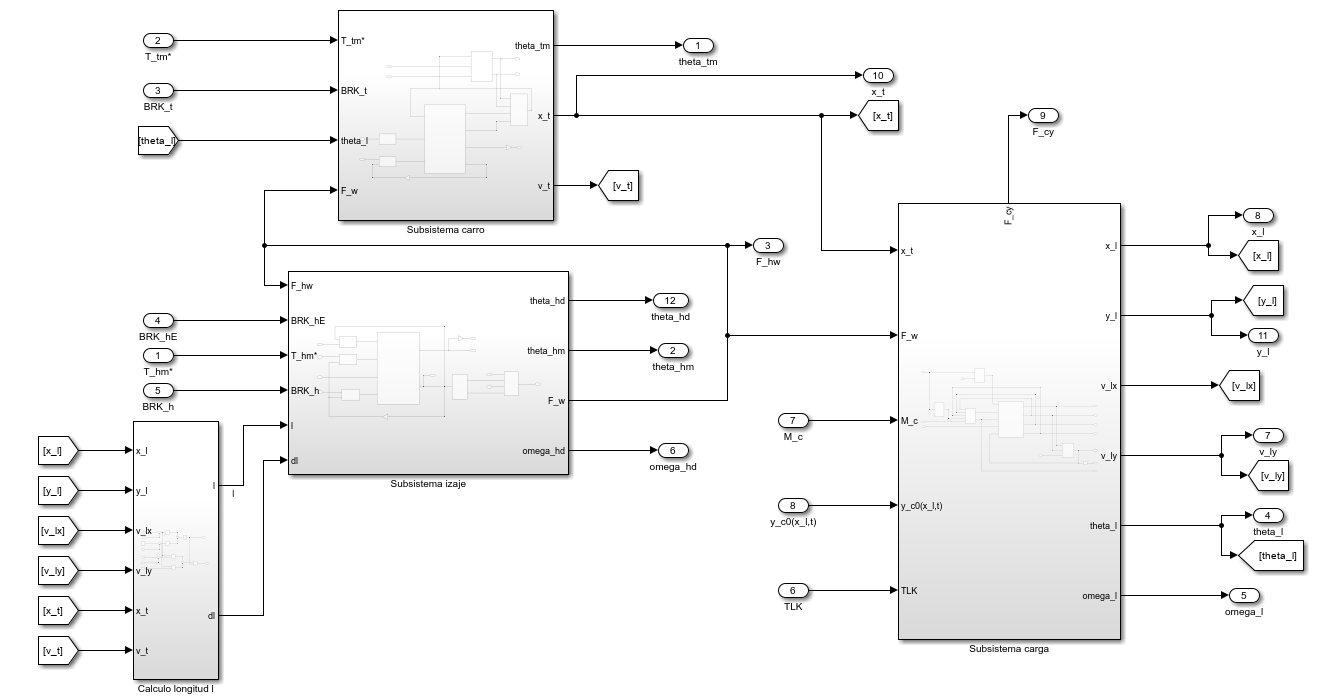
\includegraphics[width=0.95\columnwidth]{P_1.png}
\caption{Interconexión de los subsistemas de carro, izaje y carga dentro de \texttt{Planta}.}
\label{fig:planta_general}
\end{figure}

\subsection{Carga suspendida: geometría y masa}
El bloque de geometría obtiene la longitud y el ángulo a partir de las posiciones calculadas por la dinámica, sin imponer una aproximación de ángulo pequeño:
\begin{align}
l&=\sqrt{(x_l-x_t)^2+(Y_{t0}-y_l)^2},\label{eq:l}\\
\dot l&=\frac{(x_l-x_t)(v_{lx}-v_t)-(Y_{t0}-y_l)v_{ly}}{l},\label{eq:ldot}\\
\theta_l&=\operatorname{atan2}(x_l-x_t,Y_{t0}-y_l).\label{eq:theta}
\end{align}
De forma equivalente, $x_l=x_t+l\sin\theta_l$ e $y_l=Y_{t0}-l\cos\theta_l$. La función de cuatro cuadrantes conserva el signo del balanceo. Las señales $l$ y $\dot l$ alimentan el modelo del cable de izaje; $\theta_l$ determina la dirección de la tensión y se entrega al regulador de balanceo.

\begin{figure}[htbp]
\centering
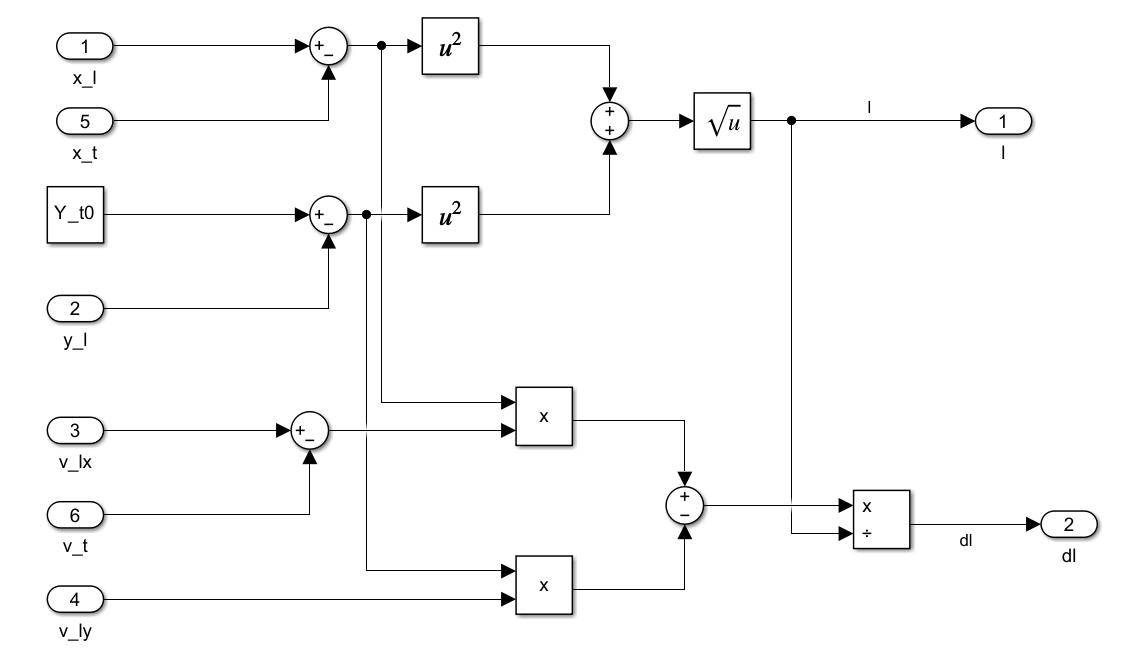
\includegraphics[width=0.88\columnwidth]{P_long1.png}
\caption{Cálculo de $l$ y $\dot l$ a partir de posiciones y velocidades relativas.}
\label{fig:longitud_cable}
\end{figure}
\begin{figure}[htbp]
\centering
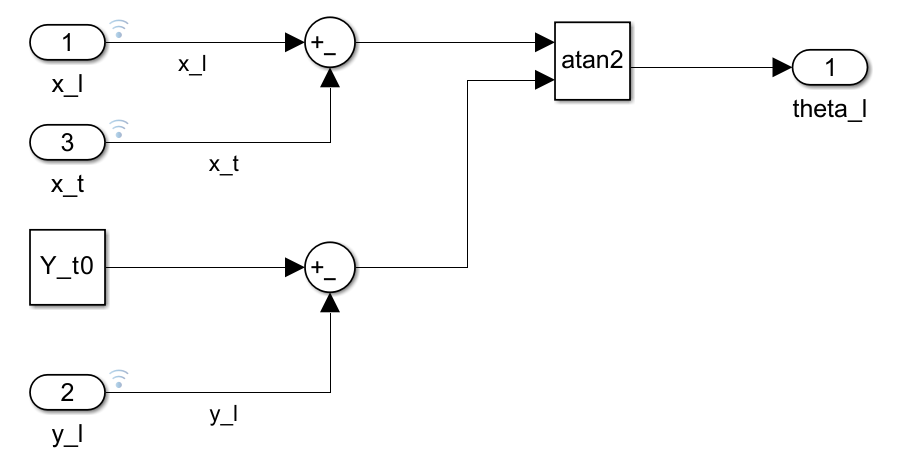
\includegraphics[width=0.75\columnwidth]{P_carga4sw_.png}
\caption{Cálculo de $\theta_l$ mediante \texttt{atan2} en el subsistema de carga.}
\label{fig:angulo_carga}
\end{figure}

La masa que interviene en los balances de fuerzas depende de la sujeción del contenedor. Con el \textit{spreader} vacío, $m_l=M_s$ y la altura inferior adicional es $h_c=0$; con el contenedor asegurado, $m_l=M_s+M_c$ y $h_c=H_c$. Se utilizan $M_s=15000~\mathrm{kg}$ y $H_c=2.59~\mathrm{m}$. Esta selección se realiza en el bloque de masa y longitud inferior del subsistema de carga. La estimación de $M_c$ a partir de la tensión, que sirve a la supervisión, se explica junto con esa función de control.

\subsection{Carga suspendida: contacto y movimiento}
El perfil $y_{c0}(x_l,t)$ representa la cota de apoyo bajo la carga. La base se encuentra en $y_l-h_c$ y la penetración calculada es $\delta=y_{c0}(x_l,t)-(y_l-h_c)$. Mientras $\delta<0$ no se aplica fuerza de contacto. Para $\delta\geq0$, el bloque utiliza una reacción vertical elástica amortiguada y una fuerza horizontal que se opone al arrastre:
\begin{align}
F_{cx}&=-b_{cx}v_{lx},\\
F_{cy}&=K_{cy}\delta-b_{cy}v_{ly}.
\end{align}
Se emplean $K_{cy}=1.8\times10^9~\mathrm{N/m}$, $b_{cy}=10\times10^6~\mathrm{N\,s/m}$ y $b_{cx}=1\times10^6~\mathrm{N\,s/m}$. La conmutación por contacto hace que ambas fuerzas sean nulas fuera del apoyo. El perfil que alimenta este bloque y su actualización durante la operación se describen en la \cref{sec:entorno_planta}.

\begin{figure}[htbp]
\centering
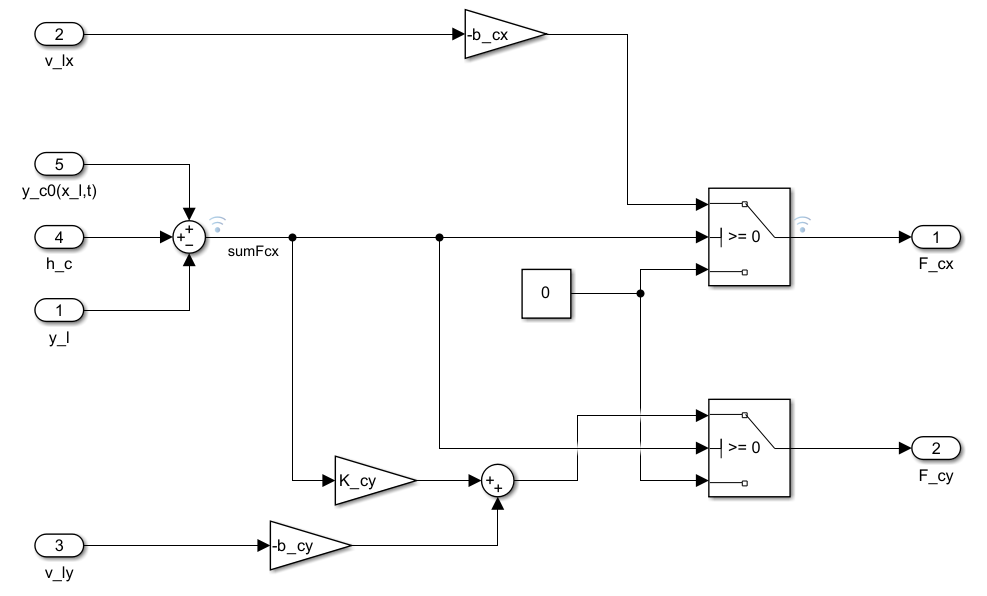
\includegraphics[width=0.86\columnwidth]{P_carga3contacto_.png}
\caption{Cálculo y conmutación de las fuerzas de contacto a partir de la penetración de la base.}
\label{fig:contacto_carga}
\end{figure}

La fuerza del cable se proyecta según el ángulo instantáneo. Los balances que implementa el bloque de movimiento son
\begin{align}
m_l\dot v_{lx}&=-2F_{hw}\sin\theta_l+F_{cx},\label{eq:loadx}\\
m_l\dot v_{ly}&=2F_{hw}\cos\theta_l+F_{cy}-m_lg.\label{eq:loady}
\end{align}
Dos integraciones sucesivas en cada eje entregan $v_{lx},x_l$ y $v_{ly},y_l$. El factor dos corresponde a los ramales equivalentes de la formulación; $F_{hw}$ es la tensión de uno de ellos. Las posiciones vuelven al cálculo geométrico, cerrando el acoplamiento entre movimiento y tensión.

\begin{figure}[htbp]
\centering
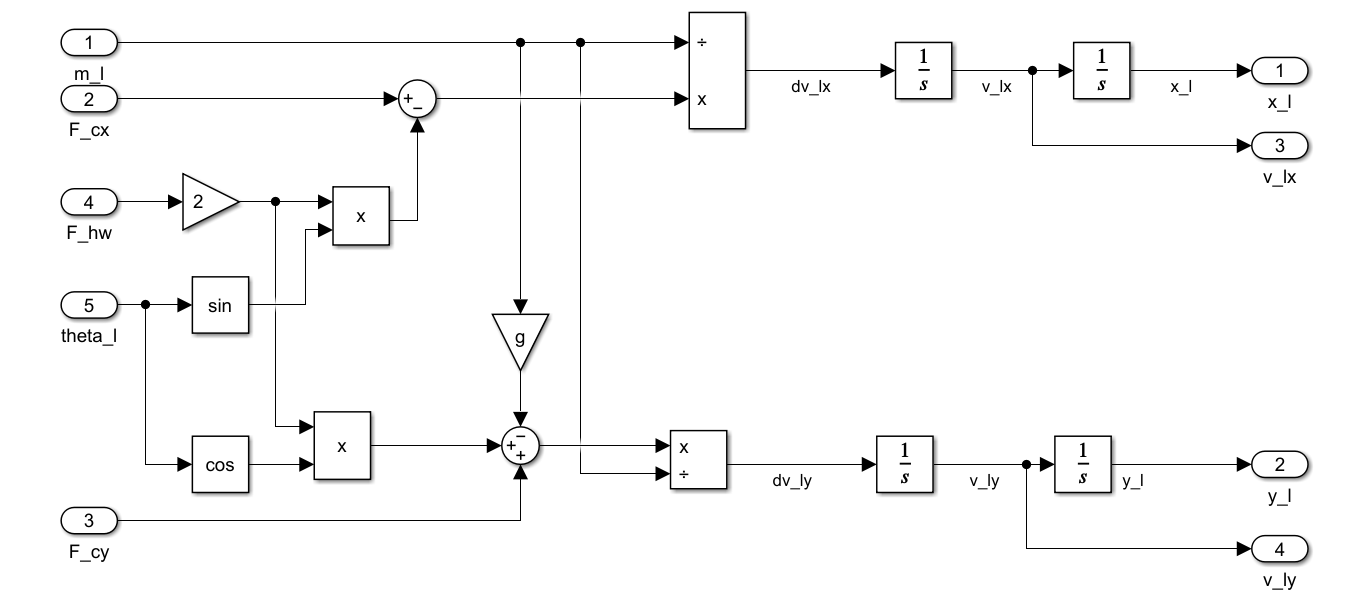
\includegraphics[width=0.94\columnwidth]{P_carga2din_.png}
\caption{Balances de fuerzas e integradores de velocidad y posición de la carga.}
\label{fig:dinamica_carga}
\end{figure}

\subsection{Izaje: cable, longitud y tambor}
Se distinguen la longitud geométrica $l$ y la longitud $l_h$ impuesta por el movimiento del tambor. La diferencia entre ambas produce la elongación del cable. Cuando el cable está tenso, la tensión por ramal se calcula como
\begin{equation}
F_{hw}=2K_{hw}(l_h)(l-l_h)+2b_{hw}(l_h)(\dot l-\dot l_h),\label{eq:rope}
\end{equation}
con $K_{hw}(l_h)=k_{hwu}/(2l_h+L_{h0})$ y $b_{hw}(l_h)=b_{hwu}(2l_h+L_{h0})$. En la condición de cable flojo se impone $F_{hw}=0$: el cable transmite tracción, pero no compresión. Los parámetros principales son $k_{hwu}=236\times10^6~\mathrm{N}$, $b_{hwu}=150~\mathrm{N\,s/m^2}$ y $L_{h0}=110~\mathrm{m}$.

En equilibrio cuasiestático, la elongación aproximada es
\begin{equation}
\Delta l\simeq\frac{m_lg}{4K_{hw}}.\label{eq:stretch}
\end{equation}
Esta estimación se usa más adelante al calcular el despeje de la trayectoria.

La relación cinemática $y_h=Y_{t0}-l_h$ implica $v_h=-\dot l_h$. Para el aparejo equivalente, $2v_h=r_{hd}\omega_{hd}$ y el torque resistente en el tambor es $T_{hdl}=F_{hw}r_{hd}$. Esta cadena transforma la rotación del tambor en una variación de longitud y devuelve la tensión como carga mecánica del accionamiento.

\begin{figure}[htbp]
\centering
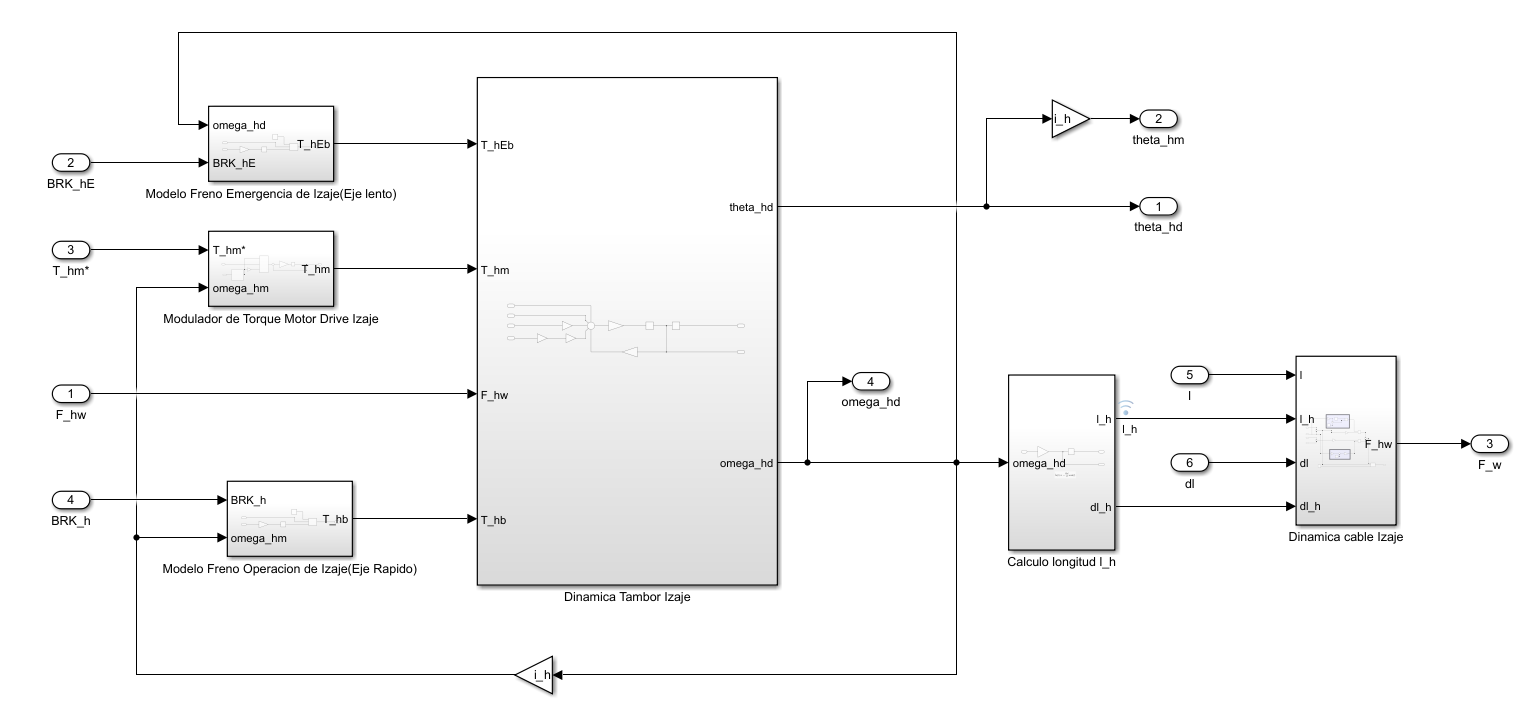
\includegraphics[width=0.94\columnwidth]{P_izj1.png}
\caption{Cadena de izaje: accionamiento, tambor, longitud comandada y cable elástico.}
\label{fig:izaje_general}
\end{figure}

\subsection{Izaje: accionamiento y frenado}
El subsistema de izaje representa el eje lento del tambor, el reductor y el eje rápido del motor. Sus balances incluyen inercia, rozamiento, torque motor, torque resistente del cable y los torques de freno. La transmisión ideal utiliza $\omega_{hm}=i_h\omega_{hd}$ y $T_{hd}=i_hT_{hml}$, con $i_h=22$. El modulador del motor aproxima la respuesta de torque mediante $\tau_{hm}\dot T_{hm}=T_{hm,\mathrm{lim}}^*-T_{hm}$, con $\tau_{hm}=1~\mathrm{ms}$. La consigna se limita a la capacidad del motor, incluida su reducción a velocidades superiores a la nominal.

El freno de operación actúa en el eje rápido y el de emergencia en el eje lento. Cuando están aplicados generan un torque opuesto a la rotación y limitado en magnitud; cuando están liberados su torque es nulo. Su mando y los enclavamientos para apertura o parada se explican con los autómatas. Aquí interesa que ambos torques entran en el balance mecánico del izaje, como muestra la \cref{fig:izaje_general}. Los valores principales de los accionamientos se reúnen en la \cref{tab:parametros_accionamientos}.

\subsection{Carro: cable, movimiento y accionamiento}
El tambor del carro fija una posición equivalente $x_{td}$ y una velocidad $v_{td}$. La diferencia con el movimiento real del carro produce la fuerza del cable:
\begin{equation}
F_{tw}=K_{tw}(x_{td}-x_t)+b_{tw}(v_{td}-v_t).\label{eq:trolleyrope}
\end{equation}
El balance traslacional, con $\dot x_t=v_t$, es
\begin{equation}
M_t\dot v_t=F_{tw}-b_tv_t+2F_{hw}\sin\theta_l.\label{eq:trolley}
\end{equation}
El último término es la reacción horizontal de la carga suspendida sobre el carro. Se utilizan $M_t=30000~\mathrm{kg}$, $K_{tw}=480~\mathrm{kN/m}$, $b_{tw}=3~\mathrm{kN\,s/m}$ y $b_t=90~\mathrm{N\,s/m}$.

El accionamiento transforma $\omega_{td}$ en $v_{td}=r_{td}\omega_{td}$, con $r_{td}=0.5~\mathrm{m}$, y refleja la fuerza del cable como torque resistente $T_{tdl}=F_{tw}r_{td}$. El reductor ideal relaciona $\omega_{tm}=i_t\omega_{td}$, con $i_t=30$. El motor recibe el torque limitado del modulador y el torque del freno de operación. El modelo conserva las inercias y pérdidas de tambor y motor como estados mecánicos, en lugar de reemplazarlas por una sola ganancia.

\begin{figure}[htbp]
\centering
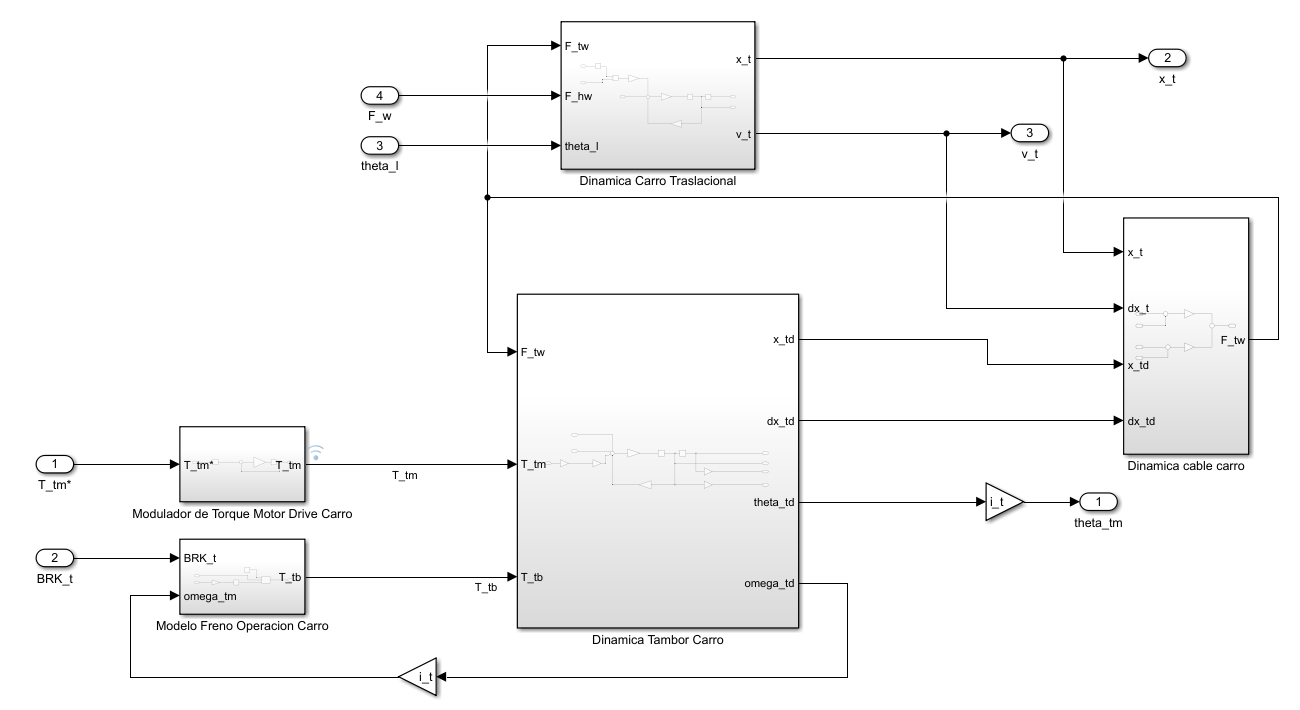
\includegraphics[width=0.94\columnwidth]{P_carro1.png}
\caption{Cadena del carro: torque, tambor, cable elástico y movimiento traslacional.}
\label{fig:carro_general}
\end{figure}

\begin{table}[htbp]
\centering
\caption{Parámetros principales de los accionamientos de la planta.}
\begin{tabular}{L{5.6cm} C{3.0cm} C{3.5cm}}
\toprule
Magnitud & Carro & Izaje\\
\midrule
Radio de tambor & $0.5~\mathrm{m}$ & $0.75~\mathrm{m}$\\
Relación de transmisión & $30$ & $22$\\
Constante de tiempo del modulador & $1~\mathrm{ms}$ & $1~\mathrm{ms}$\\
Límite nominal de torque motor & $4~\mathrm{kN\,m}$ & $20~\mathrm{kN\,m}$\\
Torque máximo del freno de operación & $5~\mathrm{kN\,m}$ & $50~\mathrm{kN\,m}$\\
Torque máximo del freno de emergencia & --- & $1.1~\mathrm{MN\,m}$\\
\bottomrule
\end{tabular}
\label{tab:parametros_accionamientos}
\end{table}

\section{Implementación en MATLAB y Simulink}
\label{sec:implementacion_planta}

\subsection{Jerarquía de subsistemas y flujo de señales}
La \cref{fig:planta_general} muestra la división de \texttt{Planta}. En \texttt{Subsistema carga} se encuentran el cálculo de masa y altura inferior, las fuerzas de contacto, el movimiento de la carga y el cálculo angular. \texttt{Subsistema izaje} comprende el tambor, la longitud comandada, el cable, el modulador de torque y los frenos. \texttt{Subsistema carro} contiene la dinámica lineal, el cable de accionamiento, el tambor, el modulador y el freno. Las señales que unen estos grupos son físicas: tensión, fuerza de cable, posiciones, velocidades y ángulo.

Las posiciones y velocidades se obtienen mediante integradores en los bloques dinámicos; las relaciones de longitud, ángulo, contacto y fuerzas se calculan algebraicamente. Los cambios de masa, apoyo, tensión y frenado seleccionan el comportamiento correspondiente sin cambiar esta organización. Las figuras de la sección anterior muestran las relaciones matemáticas directamente en los bloques que las realizan.

\subsection{Sensores y señales disponibles para el control}
La planta entrega magnitudes físicas; el subsistema \texttt{SENSORES} representa las mediciones y detecciones que utiliza el control. Los codificadores del carro y del izaje toman las posiciones angulares de sus motores, $\theta_{tm}$ y $\theta_{hm}$. En esta versión tienen ganancia unitaria, de modo que sus salidas reproducen esas posiciones sin cuantización ni ruido añadidos. El ángulo de la carga y su velocidad angular también se transmiten sin una dinámica de medición adicional.

La tensión del cable se trata de manera distinta. La celda de carga conserva la escala de $F_{hw}$ y pasa la señal por un filtro de primer orden, $G_F(s)=1/(0.1s+1)$. Así, $F_{hw,\mathrm{sens}}$ responde con un retardo de medición respecto de la tensión física utilizada en la planta. Esta diferencia importa para las condiciones de detección basadas en tensión y para la estimación de masa.

El mismo subsistema genera señales discretas a partir de variables continuas. Los finales de carrera del carro comparan $x_t$ con los límites de operación y de emergencia de ambos extremos. El detector de sobrevelocidad de izaje utiliza la velocidad obtenida del tambor y el estado de los \textit{twistlocks}, para aplicar el umbral correspondiente a la condición cargada o vacía; la captura lo identifica como el 115\,\% del límite nominal. Estas señales se entregan a los autómatas. Su lógica de respuesta se presenta en las secciones de supervisor y seguridad.

\begin{figure}[htbp]
\centering
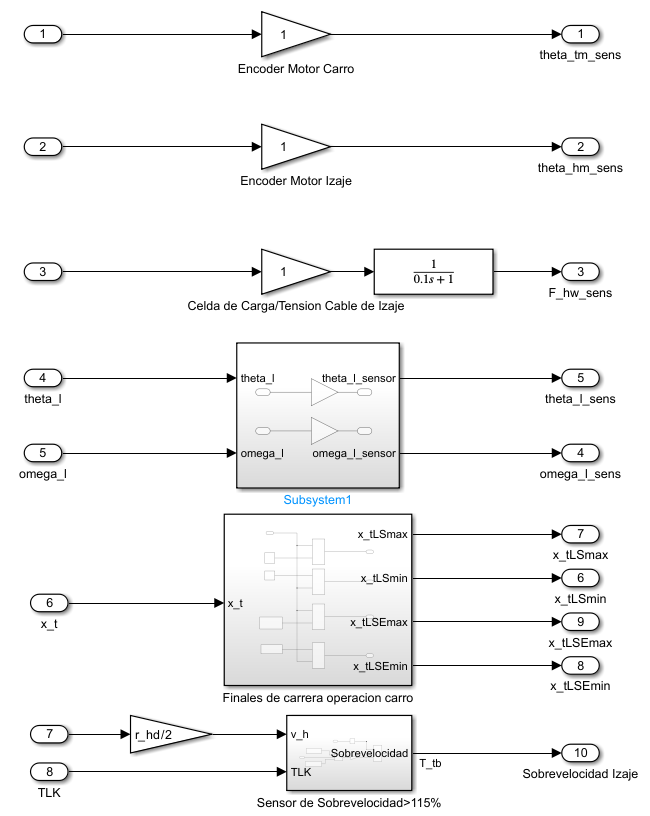
\includegraphics[width=0.78\columnwidth]{Sens_1.png}
\caption{Emulación de codificadores, celda de carga, medición angular, finales de carrera y sobrevelocidad.}
\label{fig:sensores_planta}
\end{figure}

\subsection{Perfil de obstáculos y LIDAR simulado}
\label{sec:entorno_planta}
El entorno conserva una altura de base $Z_{\mathrm{base}}(k)$ y un número de contenedores $n_k$ por cada posición discreta o \textit{slot} $k$. El ancho de un \textit{slot} es $W_c=2.44~\mathrm{m}$ y su cota se obtiene como
\begin{equation}
Y_c(k)=Z_{\mathrm{base}}(k)+n_kH_c.
\label{eq:perfil_slots}
\end{equation}
Una consulta espacial de este vector proporciona $y_{c0}(x_l,t)$ al bloque de contacto de la carga. Por ello, al modificar $n_k$, también cambia la superficie física con la que puede entrar en contacto el contenedor.

El LIDAR se simula consultando el perfil a partir de la posición del sensor. En la orientación utilizada, está $3~\mathrm{m}$ por delante del carro:
\begin{equation}
x_{\mathrm{LIDAR}}=x_t+3~\mathrm{m}.
\end{equation}
La tabla devuelve la cota asociada a esa posición y entrega las muestras de posición y altura al supervisor. El movimiento de barrido y los criterios para validar el perfil relevado se describirán con el autómata supervisor.

\subsection{Reconocimiento de toma y depósito}
La actualización del perfil necesita saber cuándo un contenedor fue realmente retirado o depositado. Para ello, el \textit{statechart} \texttt{PICK / PLACE} combina posición válida de \textit{slot}, contacto, tensión, estado de los \textit{twistlocks} y velocidad vertical. Sus estados \texttt{VACIO1} y \texttt{CARGADO1} indican si la carga está asociada al \textit{spreader}; \texttt{PRE\_PICK} y \texttt{PRE\_PLACE} conservan la información necesaria mientras se completa una toma o un depósito.

Desde \texttt{VACIO1}, el contacto con un \textit{slot} válido y los \textit{twistlocks} abiertos llevan a \texttt{PRE\_PICK}; allí se memoriza el índice del \textit{slot}. Solo cuando los \textit{twistlocks} están cerrados, hay tensión, se pierde el contacto y el conjunto asciende por encima del umbral de velocidad se confirma la toma. La transición emite \texttt{evento\_cambio}, \texttt{tipo\_evento=1} y el índice memorizado, y pasa a \texttt{CARGADO1}. Si desaparecen las condiciones de preparación, se descarta el índice y se vuelve a vacío.

Desde \texttt{CARGADO1}, el contacto con un \textit{slot} válido y la velocidad vertical próxima a cero llevan a \texttt{PRE\_PLACE}; también aquí se memoriza el lugar de apoyo. El depósito se confirma cuando se abren los \textit{twistlocks} y persiste el contacto. Se emite un único evento de tipo $2$ para ese \textit{slot} y se vuelve a \texttt{VACIO1}. Las señales de contacto y tensión se acondicionan con histéresis antes de entrar al \textit{statechart}, evitando oscilaciones de estado cerca de los umbrales. Las velocidades exigidas en las transiciones ayudan a distinguir una maniobra efectiva de un contacto momentáneo.

\begin{figure}[htbp]
\centering
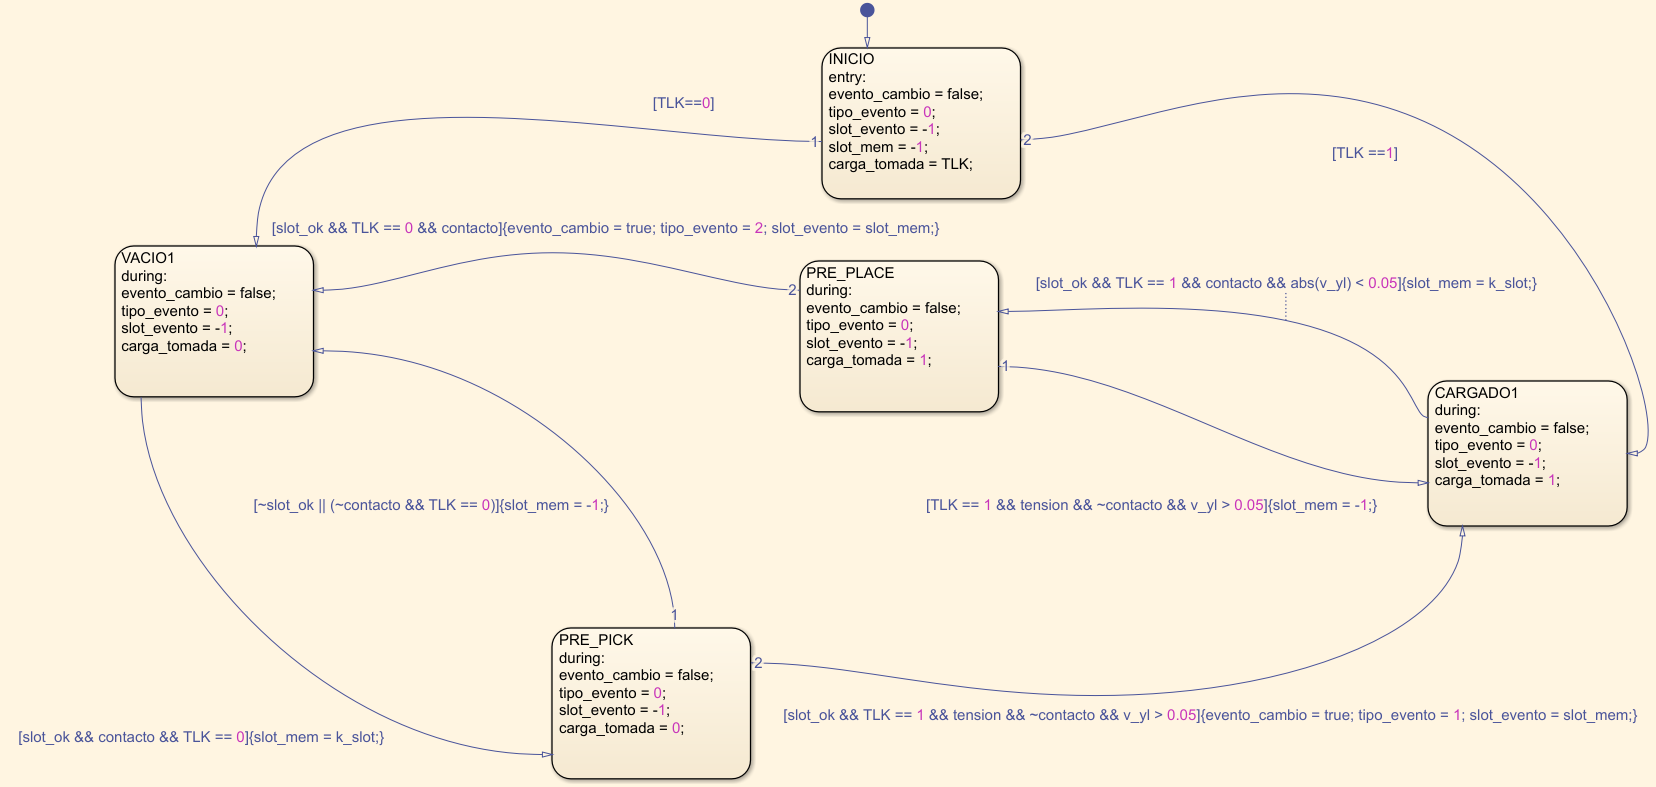
\includegraphics[width=0.98\columnwidth]{PickPlace_chart.png}
\caption{Estados y condiciones de confirmación de toma y depósito en \texttt{PICK / PLACE}.}
\label{fig:pick_place_chart}
\end{figure}

\subsection{Actualización del perfil}
Las salidas del \textit{statechart} atraviesan memorias antes de entrar a \texttt{Actualizar\_Yc}. El pulso \texttt{evento\_cambio} habilita el cambio; \texttt{tipo\_evento} indica si se retira o deposita un contenedor y \texttt{slot\_evento} identifica dónde ocurrió. El perfil actualizado alimenta la tabla espacial que entrega la altura bajo $x_l$ y retorna a la dinámica de contacto.

\begin{figure}[htbp]
\centering
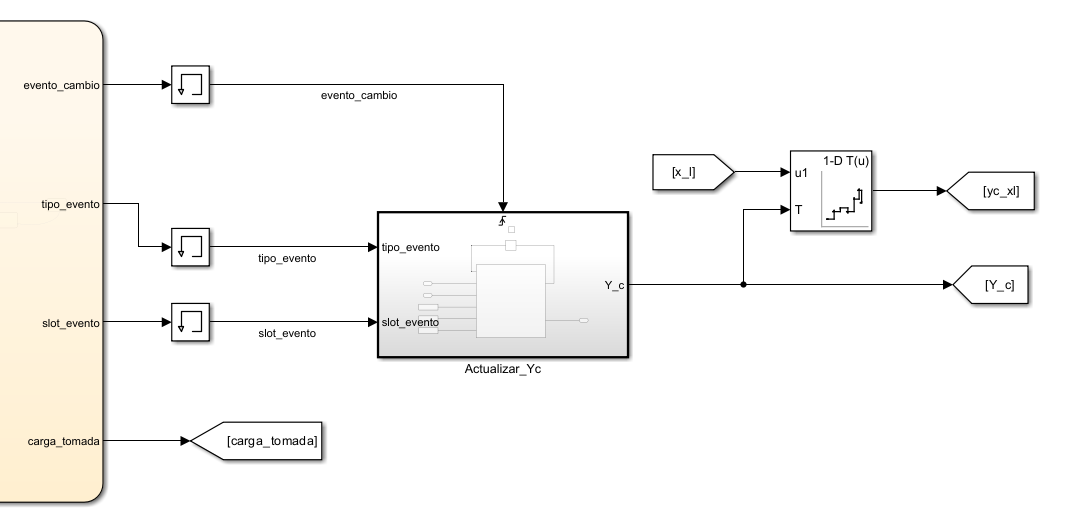
\includegraphics[width=0.91\columnwidth]{PickPlace_actObs.png}
\caption{Conexión entre el evento de \texttt{PICK / PLACE}, la actualización del perfil y su consulta espacial.}
\label{fig:actualizar_perfil_bloques}
\end{figure}

El siguiente código reproduce la función \texttt{update\_profile\_std} implementada en el bloque, omitiendo sus comentarios. Primero valida que el índice exista y que el \textit{slot} no esté bloqueado. Después reduce el número de contenedores sin permitir valores negativos, o lo incrementa si hubo un depósito. Finalmente recalcula las cotas absolutas. En los \textit{slots} bloqueados conserva la cota base; el bloqueo se representa por separado.

\begin{lstlisting}[language=Matlab,caption={Actualización del perfil de contenedores por evento.},label={lst:update_profile_std}]
function [nLevels_new, Y_c] = update_profile_std( ...
    nLevels, tipo_evento, slot_evento, ...
    Zbase, slotBlock, h_std)
Nslots = int32(length(nLevels));
nLevels_new = nLevels;
slot = int32(slot_evento);
slot_ok = (slot >= 1) && (slot <= Nslots) && (~slotBlock(slot));

if slot_ok
    if tipo_evento == 1
        nLevels_new(slot) = max(nLevels_new(slot) - 1, 0);
    elseif tipo_evento == 2
        nLevels_new(slot) = nLevels_new(slot) + 1;
    end
end

Y_c = Zbase + double(nLevels_new) * h_std;
Y_c(slotBlock) = Zbase(slotBlock);
end
\end{lstlisting}


\subsection{Configuración temporal}
La planta mecánica y los moduladores se representan con dinámica continua. El control regulatorio entrega consignas muestreadas cada $T_s=1~\mathrm{ms}$; supervisor y seguridad ejecutan su lógica cada $20~\mathrm{ms}$. Las fronteras entre estos ritmos emplean retenciones y memorias según la señal. Esta distinción permite interpretar correctamente una orden discreta de freno o cambio de carga aplicada a un modelo físico continuo.

\section{Control regulatorio}
\subsection{Estructura general}
El control del carro se organiza en cascada. El lazo exterior regula posición y entrega una corrección de velocidad. El lazo interior regula velocidad y entrega aceleración comandada. Finalmente, una compensación de dinámica calcula el torque del motor.

Para el izaje se utiliza una ley PID sobre la longitud del cable, complementada con compensaciones de masa y amortiguamiento equivalentes. Ambos controladores reciben referencias de posición, velocidad y aceleración generadas por el nivel supervisor.

% IMAGEN A INSERTAR: vista del subsistema de control regulatorio.
\figplaceholder[0.50\textheight]{Captura del subsistema que contiene \texttt{Controlador Carro}, \texttt{Balanceo completo} y \texttt{Controlador Izaje}.}{Estructura general del nivel regulatorio.}


\subsection{Lazo de posición del carro}
La referencia base de velocidad se corrige con un término proporcional al error de posición:
\begin{equation}
v_{pos}=v_{ff}+K_x(x_t^*-x_{td}).
\label{eq:posloop}
\end{equation}
Se utiliza la posición del tambor $x_{td}$, disponible a partir del codificador. La ganancia seleccionada es
\begin{equation}
K_x=0.2~\mathrm{s^{-1}}.
\end{equation}
La salida se limita a $\pm4~\mathrm{m/s}$. El término $v_{ff}$ permite que el lazo no deba generar por error toda la velocidad de la trayectoria. La realimentación corrige diferencias producidas por la elasticidad, las perturbaciones y las saturaciones.

% IMAGEN A INSERTAR: lazo de posición del Controlador Carro.
\figplaceholder{Detalle del error de posición, ganancia $K_x$, suma con \textit{feedforward} y saturación.}{Lazo exterior de posición del carro.}


\subsection{Lazo de velocidad del carro}
El error de velocidad se define como
\begin{equation}
e_v=v_{ref}-v_{td}.
\end{equation}
La aceleración de corrección es
\begin{equation}
a_{PI}=K_{pv}e_v+K_{iv}\int e_v\,dt,
\label{eq:velocitypi}
\end{equation}
con $K_{pv}=2.40~\mathrm{s^{-1}}$ y $K_{iv}=0.20~\mathrm{s^{-2}}$. Para la planta compensada $v/a_{cmd}\simeq1/s$, el polinomio nominal es
\begin{equation}
s^2+K_{pv}s+K_{iv}.
\end{equation}
La sintonía es deliberadamente sobreamortiguada. Se privilegia un seguimiento sin sobrepasos grandes, porque un exceso de velocidad aumenta el ángulo y puede llevar el torque a saturación.

% IMAGEN A INSERTAR: lazo PI de velocidad con integrador discreto.
\figplaceholder{Detalle del error de velocidad, $K_{pv}$, $K_{iv}$ y el integrador discreto con $T_s=1~\mathrm{ms}$.}{Lazo interior de velocidad del carro.}


\subsection{Compensación de dinámica del carro}
La aceleración total solicitada es la suma de la aceleración de trayectoria y la salida del PI. A partir de \eqref{eq:trolley} se construye una compensación de torque de la forma
\begin{equation}
T_{tm}^*=\frac{r_{td}M_{EQt}}{i_t}\left[a_{cmd}+\frac{b_{EQt}}{M_{EQt}}v_{td}-\frac{2F_{hw}}{M_{EQt}}\sin\theta_l\right].
\label{eq:computedtorque}
\end{equation}
El último término compensa la componente horizontal de la tensión. La compensación no elimina las saturaciones ni las dinámicas flexibles del modelo completo; solamente reduce la carga que deben soportar los términos de realimentación.

% IMAGEN A INSERTAR: subsistema Computed Torque.
\figplaceholder{Captura del subsistema \texttt{Computed Torque}, con los términos de inercia, fricción y tensión horizontal.}{Compensación de dinámica del carro.}


\subsection{Referencia angular y compensación anti-sway}
La aceleración horizontal de referencia determina un ángulo cuasiestático:
\begin{equation}
\theta_l^*=\operatorname{atan2}(-a_{ff},g).
\label{eq:thetaref}
\end{equation}
El error angular se transforma en una corrección de velocidad:
\begin{equation}
v_{sw}=2\zeta_{sw}\sqrt{gl_h}(\theta_l-\theta_l^*).
\label{eq:antisway}
\end{equation}
La corrección se limita antes de sumarse a la referencia principal. La sintonía de base utiliza $\zeta_{sw}=1.4$ y un límite de $1.4~\mathrm{m/s}$. El factor $\sqrt{g/l_h}$ representa la variación de frecuencia natural con la longitud del péndulo; escrito como en \eqref{eq:antisway}, el término convierte el error angular en velocidad.

% IMAGEN A INSERTAR: bloque Balanceo_completo y generación theta referencia.
\figplaceholder{Detalle de $\theta_l^*$, error angular, dependencia con $l_h$ y limitación de $v_{sw}$.}{Compensación de balanceo de la carga.}


\subsection{Habilitación anti-sway y espera antes del descenso}
En \texttt{PLANIFICAR}, \texttt{EJECUTAR} y \texttt{MANTENER\_OBJETIVO}, el supervisor asigna \texttt{swayControlEnable} según \texttt{swayControlSelect}. Por lo tanto, la versión vigente mantiene el anti-sway seleccionado durante el traslado y no lo deshabilita por alcanzar la velocidad productiva o por cruzar la línea global de seguridad.

El perfil horizontal admite una velocidad máxima de diseño de $2.5~\mathrm{m/s}$. Cuando el descenso final se programa al terminar la traslación, el reloj del generador se retiene en el instante de inicio del descenso hasta que se cumplen simultáneamente
\begin{align}
|x_t-x_t^*|&\leq0.08~\mathrm{m},\\
|v_t|&\leq0.06~\mathrm{m/s},\\
|\theta_l|&\leq0.005~\mathrm{rad},\\
|\dot\theta_l|&\leq0.012~\mathrm{rad/s}.
\end{align}
Estas condiciones pertenecen a \texttt{craneTrajectoryGenerator}; no se agregan a la transición del chart \texttt{EJECUTAR} hacia \texttt{MANTENER\_OBJETIVO}, que conserva sus tolerancias de posición. La espera se aplica cuando \texttt{yDownStart} es mayor o igual que la duración horizontal, dentro de la tolerancia numérica del generador. En la comparación sin anti-sway estas condiciones siguen activas.

% IMAGEN A INSERTAR: curvas de velocidad, ángulo y habilitación anti-sway durante una transferencia.
\figplaceholder{Gráficas temporales de $v_t$, $v_t^*$, $\theta_l$ y la señal de habilitación anti-sway.}{Habilitación anti-sway y condiciones de espera antes del descenso.}


\subsection{Control del izaje}
El controlador de izaje actúa sobre la longitud $l_h$, cuya referencia se obtiene de la posición vertical. La ley implementada combina los errores de longitud, velocidad y una acción integral:
\begin{equation}
u_h=K_{hp}e_l+K_{hd}e_{\dot l}+K_{hi}\int e_l\,dt+u_{ff}.
\end{equation}
Las ganancias se calculan a partir de los parámetros equivalentes:
\begin{align}
K_{hp}&=-\frac{r_{hd}M_{EQh}n_h\omega_{posh}^2}{i_h},\\
K_{hi}&=-\frac{r_{hd}M_{EQh}\omega_{posh}^3}{i_h},\\
K_{hd}&=\frac{r_{hd}}{i_h}(b_{EQh}-M_{EQh}n_h\omega_{posh}).
\end{align}
Se seleccionan $n_h=2.7$ y $\omega_{posh}=1.8~\mathrm{rad/s}$.

% IMAGEN A INSERTAR: Controlador Izaje completo.
\figplaceholder{Captura del controlador de izaje, incluyendo errores, integradores Tustin y compensaciones.}{Estructura del regulador de izaje.}


\subsection{Cierre adicional de posición vertical}
El generador entrega un perfil vertical planificado, pero se agrega una corrección para evitar que los errores acumulados impidan alcanzar la cota final. La velocidad comandada es
\begin{equation}
v_{h,cmd}=\operatorname{sat}\left(v_{h,plan}+K_y e_y\right),
\end{equation}
con una zona muerta de $0.05~\mathrm{m}$ y $K_y=0.60~\mathrm{s^{-1}}$. Con carga se limita la velocidad a $0.30~\mathrm{m/s}$ en la trayectoria automática y la corrección a $0.20~\mathrm{m/s}$. Sin carga se admiten hasta $3~\mathrm{m/s}$.

La referencia de aceleración se limita a $\pm0.05~\mathrm{m/s^2}$ durante la maniobra automática. Esta restricción conserva tensión en el cable y evita que un descenso rápido genere cuerda floja.

% IMAGEN A INSERTAR: señales de referencia y medida del izaje.
\figplaceholder{Gráficas de $y_h$, $y_h^*$, $v_h$ y $v_h^*$ durante la maniobra.}{Seguimiento de las referencias de izaje.}


\subsection{Transferencias sin salto}
La transferencia desde manual hacia automático se realiza mediante estados específicos; existe además una entrada directa desde \texttt{LISTO} hacia \texttt{AUTOMATICO}. En \texttt{BUMPLESS\_A\_AUTO}, las referencias se inicializan con la posición, velocidad y aceleración medidas. Después de dos ciclos del supervisor se habilita el generador automático.

En \texttt{BUMPLESS\_A\_MANUAL}, las velocidades objetivo se alcanzan con rampas limitadas a $0.8~\mathrm{m/s^2}$ para el carro y $0.75~\mathrm{m/s^2}$ para el izaje. El cambio final a manual ocurre con el sistema prácticamente detenido. Esta estrategia evita saltos de torque y mantiene continuidad en las consignas.

% IMAGEN A INSERTAR: curvas alrededor de un cambio manual/automático/manual.
\figplaceholder{Gráficas ampliadas de referencias y variables medidas durante ambos cambios de modo.}{Transferencias sin salto entre modos de operación.}


\section{Generación de trayectorias}
\subsection{Objetivo de la planificación}
En modo automático el operador proporciona principalmente la posición horizontal final. La función de envolvente local dilata el perfil relevado tomando el máximo de cada celda y sus vecinas inmediatas. La función de superficie objetivo consulta el máximo de las celdas de esa envolvente solapadas por el ancho de $2.44~\mathrm{m}$ del contenedor. La altura de aproximación se obtiene como
\begin{equation}
y_{auto}=y_{env}(x^*)+H_c(1+\delta_{carga})+\Delta l_{est},\qquad H_c=2.59~\mathrm{m},
\label{eq:objetivo_local_vigente}
\end{equation}
donde $\delta_{carga}$ vale uno con contenedor y cero con \textit{spreader} vacío. El estiramiento se calcula con la masa suspendida limitada entre $15000$ y $65000~\mathrm{kg}$ y la rigidez del cable evaluada a partir de la altura base. Esta revisión utiliza un margen fijo de una altura de contenedor; \texttt{finalApproachDistance} permanece en la interfaz, pero no interviene en \texttt{calcularObjetivoSeguro}.

La trayectoria automática debe elevar y trasladar simultáneamente, respetar las cotas de obstáculos y terminar con velocidad y aceleración nulas.

% IMAGEN A INSERTAR: perfil con origen, destino, línea de seguridad y envolvente de carga.
\figplaceholder{Esquema del origen, destino, obstáculo máximo, línea de seguridad y altura de aproximación.}{Magnitudes utilizadas por el planificador.}


\subsection{Línea de seguridad}
La línea de seguridad implementada se calcula mediante
\begin{equation}
y_{seg}=\max\left(y_{manual\rightarrow auto},\min(40,\max_i y_{perfil,i}+2H_c)\right).
\label{eq:safetyline}
\end{equation}
El desplazamiento de dos alturas de contenedor equivale a $5.18~\mathrm{m}$. La línea se dibuja en la visualización y permite calcular \texttt{clearanceOK}, pero esta bandera no se utiliza en las guardas de entrada al automático ni para deshabilitar el anti-sway. El generador conserva además una cota alta de cruce no menor que el máximo de la envolvente más $5.18~\mathrm{m}$.

Para verificar el despeje se descuenta el estiramiento del cable calculado con \eqref{eq:stretch}. La condición calculada por \texttt{calcularDespeje} es
\begin{equation}
y_l-\Delta l\geq y_{seg}.
\end{equation}
Esta comprobación global se distingue de \texttt{autoEntryHeightOK}, que compara la altura medida del izaje con \texttt{calcularObjetivoSeguro} evaluado en la posición actual del carro.

% IMAGEN A INSERTAR: HMI con línea de seguridad visible.
\figplaceholder[0.50\textheight]{Captura de la visualización HMI mostrando la línea horizontal de seguridad y su valor numérico.}{Representación de la línea de seguridad en la visualización.}


\subsection{Perfil horizontal}
El movimiento horizontal utiliza rampas senoidales de aceleración, un tramo de velocidad constante y una rampa de frenado. Se adoptan
\begin{equation}
v_{x\max}=2.5~\mathrm{m/s},\quad a_{x\max}=0.3~\mathrm{m/s^2},\quad j_{x\max}=0.5~\mathrm{m/s^3}.
\end{equation}
Si la distancia es suficiente, el perfil alcanza la velocidad máxima. Si es corta, se reduce la velocidad de crucero. La duración de la rampa se selecciona como
\begin{equation}
T_r=\max\left(0.25,\frac{\pi v_c}{2a_{x\max}},\pi\sqrt{\frac{v_c}{2j_{x\max}}}\right).
\end{equation}
Las rampas senoidales hacen que la aceleración comience y termine en cero, reduciendo la excitación de la carga suspendida.

% IMAGEN A INSERTAR: perfiles x, v, a y jerk horizontales.
\figplaceholder{Gráficas del perfil horizontal de posición, velocidad, aceleración y \textit{jerk}.}{Perfil de traslación del carro.}


\subsection{Perfil vertical quíntico}
Para el izaje se utilizan polinomios de quinto orden:
\begin{equation}
p(t)=c_0+c_1t+c_2t^2+c_3t^3+c_4t^4+c_5t^5.
\end{equation}
Los coeficientes se calculan imponiendo posición, velocidad y aceleración inicial y final. La duración mínima se busca de forma iterativa hasta verificar los límites de velocidad, aceleración y \textit{jerk}. Se utilizan $a_{y\max}=0.25~\mathrm{m/s^2}$ y $j_{y\max}=0.10~\mathrm{m/s^3}$ para el movimiento automático. El límite de $0.05~\mathrm{m/s^2}$ corresponde a la aproximación final manual.

El perfil vertical se divide en una fase ascendente y otra descendente. La fase de descenso comienza cuando la envolvente horizontal abandonó la zona de obstáculos y el carro está en condiciones de posicionamiento.

% IMAGEN A INSERTAR: perfiles y, vy, ay y jerk del izaje.
\figplaceholder{Gráficas del perfil quíntico vertical y sus tres primeras derivadas.}{Perfil vertical utilizado por el planificador.}


\subsection{Coordinación simultánea}
El movimiento horizontal y el izaje comienzan en $t=0$. Antes de aceptar el plan se muestrea la trayectoria y se verifica que la base de la carga se mantenga por encima del perfil más el margen vertical. Si el carro alcanzaría un obstáculo demasiado pronto, se aumenta la duración horizontal por un factor $1.025$ y se repite la verificación.

Este procedimiento no demora intencionalmente el inicio del carro. En cambio, reduce su avance solamente lo necesario para que el izaje gane altura. Una vez alcanzada la zona libre, la trayectoria recupera el tramo de velocidad constante. Con esto se mejora el tiempo de ciclo respecto de una secuencia puramente escalonada de elevar, trasladar y descender.

% IMAGEN A INSERTAR: secuencia de posiciones superpuestas o diagrama x-y de la trayectoria.
\figplaceholder[0.50\textheight]{Trayectoria en el plano $x$--$y$ con varios instantes de la carga y el perfil de obstáculos.}{Coordinación simultánea de izaje y traslación.}


\subsection{Verificación de colisión}
La envolvente horizontal se amplía con medio ancho de contenedor y un margen adicional de $2.59~\mathrm{m}$. El margen vertical \texttt{VERTICAL\_MARGIN} también vale $2.59~\mathrm{m}$ en el generador vigente. En cada muestra del plan se calcula la cota del obstáculo debajo de la carga. La condición de seguridad es
\begin{equation}
y_l-\Delta l-h_c\geq y_{obs}(x_l)+d_v.
\end{equation}
El plan se declara inválido si no puede cumplir esta condición antes del tiempo máximo. En ese caso, las referencias se fijan en el estado medido y no se genera movimiento automático.

Este comportamiento es preferible a saturar la altura o ignorar un obstáculo, porque una trayectoria inviable queda convertida en una condición detenida y observable por el supervisor.

% IMAGEN A INSERTAR: detalle de la envolvente de colisión sobre el perfil.
\figplaceholder{Esquema de la base del contenedor, estiramiento del cable, margen vertical y perfil de obstáculos.}{Criterio geométrico de ausencia de colisión.}


\clearpage
\section{Autómata supervisor}
\subsection{Estructura general}
El autómata supervisor se implementa como un diagrama Stateflow con cinco regiones paralelas. La región \texttt{INTERLOCKS} se ejecuta en primer lugar y acondiciona las entradas, calcula aceleraciones, límites normales, comprobaciones de torque, códigos auxiliares y banderas comunes. En segundo lugar se ejecuta \texttt{CARGA\_Y\_TWISTLOCKS}, que controla la toma, el pesaje y la liberación. \texttt{OPERACION} se ejecuta en tercer lugar y administra los modos principales. Luego se ejecuta \texttt{FRENOS}, que contiene en paralelo las máquinas del carro y del izaje. Finalmente, \texttt{DIAGNOSTICO} actualiza los códigos de alarma y falla.

El paralelismo permite que las secuencias de carga y frenos continúen supervisándose mientras cambia el modo de operación. Las regiones comparten variables locales y salidas; por ello, el orden indicado resulta relevante. En particular, \texttt{INTERLOCKS} calcula las banderas que posteriormente consumen las regiones de carga, operación y diagnóstico durante la misma activación del chart.

\begin{figure}[!htbp]
    \centering
    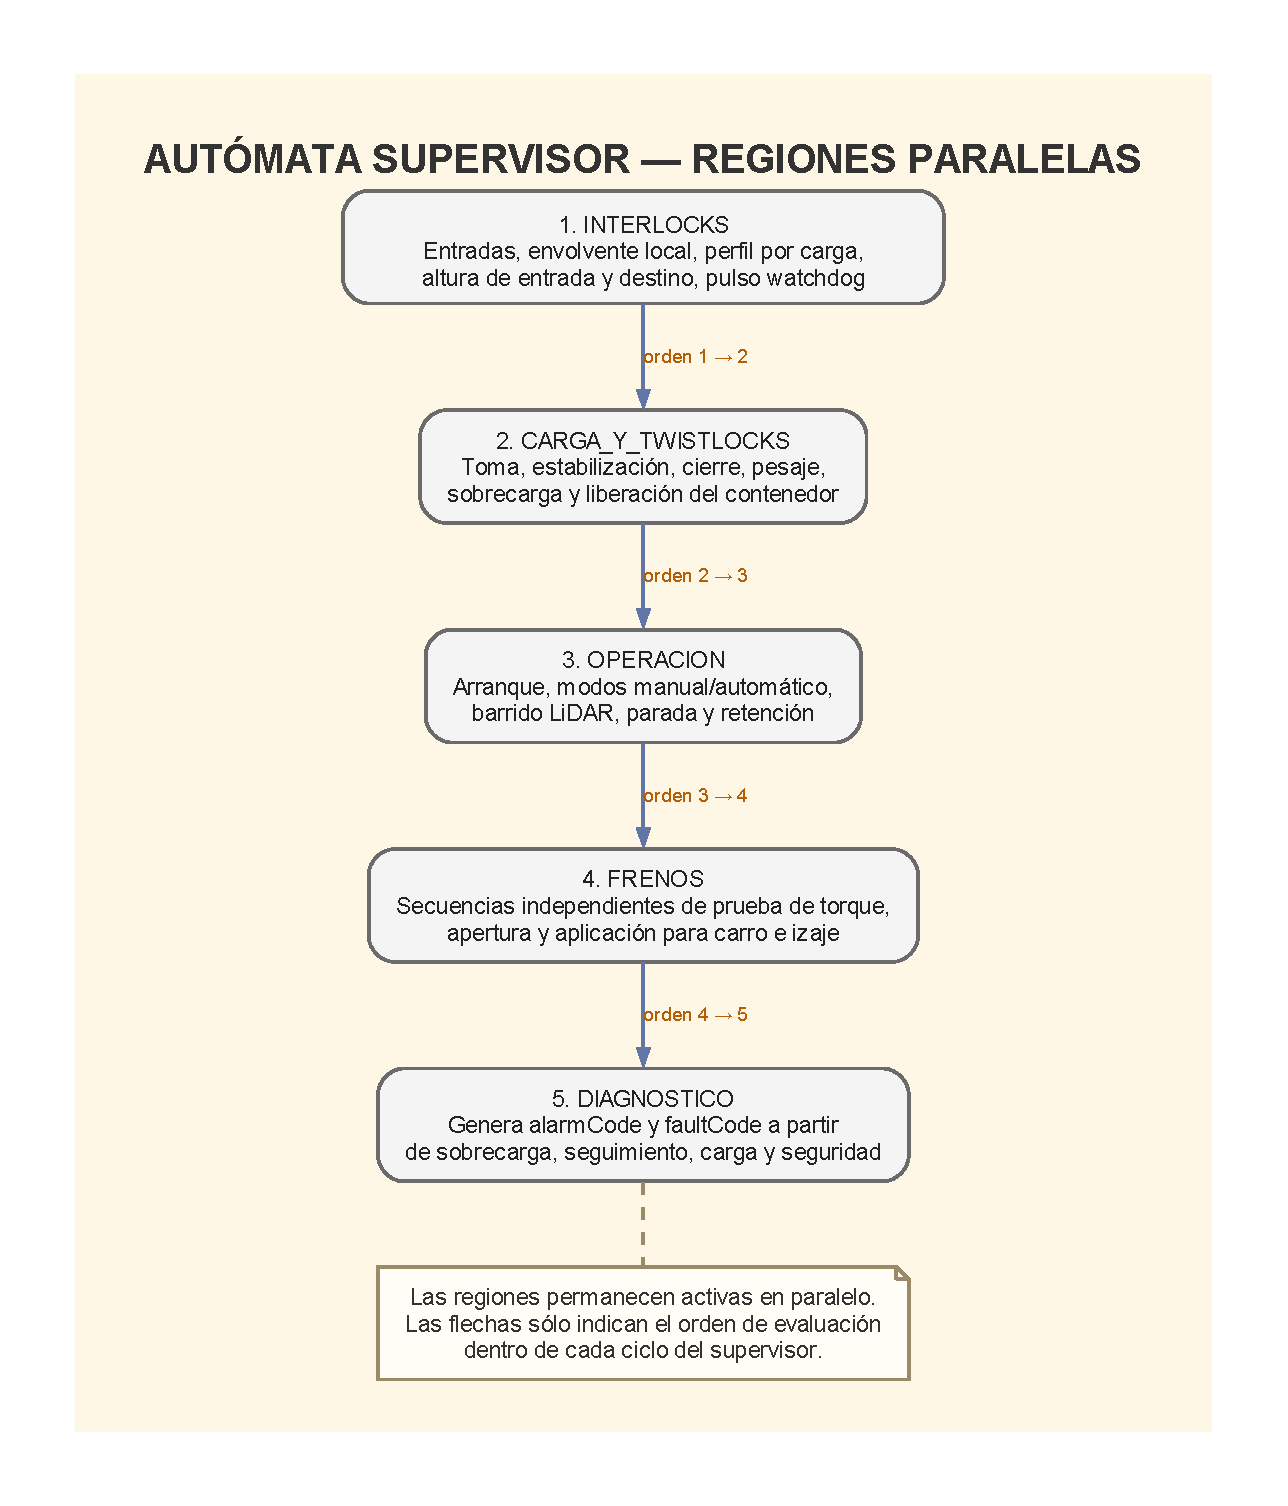
\includegraphics[height=0.72\textheight,keepaspectratio]{diagramas_automatas_revision/01_arquitectura_supervisor.pdf}
    \caption{Organización general, responsabilidades y orden de ejecución de las regiones paralelas del autómata supervisor.}
\end{figure}


\subsection{Interfaz funcional del supervisor}
El supervisor constituye el vínculo entre las órdenes del operador, las mediciones de la planta, el nivel de seguridad y los reguladores. Sus entradas no representan mandos directos sobre los actuadores: se procesan para obtener condiciones lógicas, referencias limitadas y permisos internos. La \cref{tab:interfaz_supervisor} resume las señales que determinan las decisiones principales.

\begin{longtable}{L{4.1cm} L{4.2cm} L{5.3cm}}
\caption{Interfaz funcional principal del autómata supervisor.}\label{tab:interfaz_supervisor}\\
\toprule
Grupo & Señales representativas & Utilización dentro del supervisor\\
\midrule
\endfirsthead
\toprule
Grupo & Señales representativas & Utilización dentro del supervisor\\
\midrule
\endhead
Órdenes & Marcha, parada, reinicio, selección manual/automática y orden de barrido & Selección de estados operativos y reconocimiento de fallas.\\
Mandos manuales & \textit{Joystick} horizontal, \textit{joystick} vertical y órdenes de \textit{twistlocks} & Generación de referencias manuales y secuencia de toma o liberación.\\
Movimiento & Posición, velocidad y aceleración de carro e izaje & Seguimiento de trayectoria, transferencias sin salto y aplicación de frenos.\\
Carga suspendida & Ángulo, velocidad angular, tensión, contacto y confirmación de \textit{twistlocks} & Estabilización, pesaje, detección de cuerda floja y estado de carga.\\
Perfil & Posición del LIDAR, altura medida y memoria del perfil & Registro del barrido, validación de cobertura y cálculo de la superficie objetivo.\\
Seguridad & Permisos global, de carro y de izaje & Habilitación de movimientos, parada normal y retención de falla.\\
Salidas de referencia & $x^*$, $v_x^*$, $a_x^*$, $y^*$, $v_y^*$ y $a_y^*$ & Consignas entregadas al nivel regulatorio.\\
Salidas discretas & Órdenes de freno, \textit{twistlocks}, códigos, estado y pulso de \textit{watchdog} & Accionamiento secuencial, diagnóstico, HMI y vigilancia desde el nivel de seguridad.\\
\bottomrule
\end{longtable}

\subsection{Región INTERLOCKS}
La región \texttt{INTERLOCKS} concentra los cálculos que deben estar disponibles antes de evaluar las restantes regiones paralelas. No constituye una secuencia de producción independiente, sino una etapa de acondicionamiento y generación de variables comunes. Su ejecución al comienzo de cada activación evita repetir operaciones en diferentes estados y proporciona una única interpretación de las señales de entrada.

Entre sus tareas se encuentran el cálculo de aceleraciones a partir de velocidades muestreadas, la detección de flancos de órdenes, la comprobación de límites normales, la validación de torque previo a la apertura de los frenos, la evaluación del error de seguimiento, el cálculo de la altura de despeje y la actualización de códigos auxiliares. La \cref{tab:interlocks_supervisor} relaciona las funciones principales con las regiones que utilizan sus resultados.

\begin{table}[!htbp]
\centering
\caption{Resultados principales generados por \texttt{INTERLOCKS}.}\label{tab:interlocks_supervisor}
\begin{tabular}{L{4.5cm} L{5.0cm} L{4.2cm}}
\toprule
Resultado & Criterio general & Consumidor principal\\
\midrule
Aceleraciones medidas & Diferencia discreta de velocidades & Operación y trayectoria\\
Límites normales & Comparación de posición y sentido solicitado & Mando manual y barrido\\
Torque comprobado & Torque disponible durante el estado de prueba & Máquinas de freno\\
\texttt{trackingFault} & Error sostenido de seguimiento & Operación y diagnóstico\\
Altura de aproximación & Envolvente local, carga, margen y estiramiento & Automático\\
\texttt{autoEntryHeightOK} & Perfil válido y altura local suficiente & Entrada al automático\\
\texttt{clearanceOK} & Despeje respecto de la línea global & Cálculo auxiliar; no es guarda de entrada\\
Códigos auxiliares & Combinación de condiciones activas & Diagnóstico y HMI\\
\bottomrule
\end{tabular}
\end{table}

La memoria \texttt{scannedObstacleProfile} se actualiza al cambiar \texttt{loadedState}, siempre que el perfil sea válido y no exista barrido activo: se resta $2.59~\mathrm{m}$ al tomar un contenedor y se suma la misma altura al liberarlo, en la celda asociada a la posición del carro. Luego se recalcula la envolvente local. Como carga se ejecuta después de \texttt{INTERLOCKS}, el cambio de estado cargado se incorpora al perfil en la siguiente activación.

\texttt{retenerSolicitudHMI} memoriza el flanco de solicitud de barrido recibido con el escaneo inactivo y lo conserva hasta parada, reinicio o secuencia completa. Esto permite atender un pulso del HMI una vez alcanzadas las condiciones de inicio.

Las operaciones indicadas se ejecutan durante cada ciclo del supervisor. En consecuencia, una modificación de una bandera calculada en \texttt{INTERLOCKS} puede ser utilizada por las regiones de carga y operación dentro de la misma activación del chart, siempre respetando el orden de ejecución configurado.


\subsection{Indexación de estados de operación}
Para facilitar su utilización posterior se adopta la siguiente indexación funcional:
\begin{longtable}{C{1.2cm} L{4.4cm} L{8.2cm}}
\caption{Estados de la región de operación.}\\
\toprule
Índice & Estado & Función principal\\
\midrule
O0 & \texttt{APAGADO} & Deshabilita reguladores y mantiene las referencias en la posición medida.\\
O1 & \texttt{ARRANQUE} & Inicia la secuencia, conserva frenos y espera permisos estables.\\
O2 & \texttt{LISTO} & Habilita reguladores con referencias detenidas y espera una selección.\\
O3 & \texttt{MANUAL\_SUPERVISADO} & Convierte los mandos del operador en referencias limitadas.\\
O4 & \texttt{BUMPLESS\_A\_AUTO} & Inicializa referencias con el estado medido antes del automático.\\
O5 & \texttt{AUTOMATICO} & Contiene planificación, ejecución y retención del objetivo.\\
O6 & \texttt{BUMPLESS\_A\_MANUAL} & Reduce las referencias en forma continua al abandonar automático.\\
O7 & \path{APROXIMACION_FINAL_MANUAL} & Mantiene $x$ y permite el mando vertical manual.\\
O8 & \path{PREPARAR_ESCANEO_LIDAR} & Eleva el conjunto y reinicia la memoria del perfil.\\
O9 & \texttt{IR\_EXTREMO\_DERECHO} & Traslada el carro vacío al inicio del barrido.\\
O10 & \path{BARRIDO_LIDAR_IZQUIERDA} & Retorna registrando el perfil.\\
O11 & \path{FINALIZAR_ESCANEO_LIDAR} & Detiene y valida la cobertura de los 33 \textit{slots}.\\
O12 & \texttt{PARADA\_NORMAL} & Lleva velocidades a cero respetando las rampas.\\
O13 & \texttt{RETENCION\_FALLA} & Deshabilita reguladores y retiene el sistema ante una falla.\\
\bottomrule
\end{longtable}


\subsection{Estados APAGADO, ARRANQUE y LISTO}
\texttt{APAGADO} es el estado inicial. Su código de modo es cero y ambos reguladores quedan deshabilitados. La transición a \texttt{ARRANQUE} exige orden de marcha, permiso global y configuración válida.

\texttt{ARRANQUE} utiliza el código de modo uno. Durante este estado se mantiene el sistema sin referencias de movimiento y se verifica la disponibilidad de los permisos. Luego de cinco ciclos del supervisor, si carro e izaje están permitidos, se pasa a \texttt{LISTO}.

\texttt{LISTO} utiliza el código dos y habilita los reguladores con consignas detenidas. Posee transiciones hacia manual, automático, parada, retención de falla y barrido. La entrada a automático desde este estado es directa, sin pasar por \path{BUMPLESS_A_AUTO}, y exige \texttt{modeAutoReq}, \texttt{cmdAutoStart}, perfil válido, \texttt{autoEntryHeightOK} y ausencia de sobrecarga. La altura local se comprueba tanto con carga como con \textit{spreader} vacío; esta transición no exige \texttt{loadedState} ni ausencia de intervención manual.

\begin{figure}[!htbp]
    \centering
    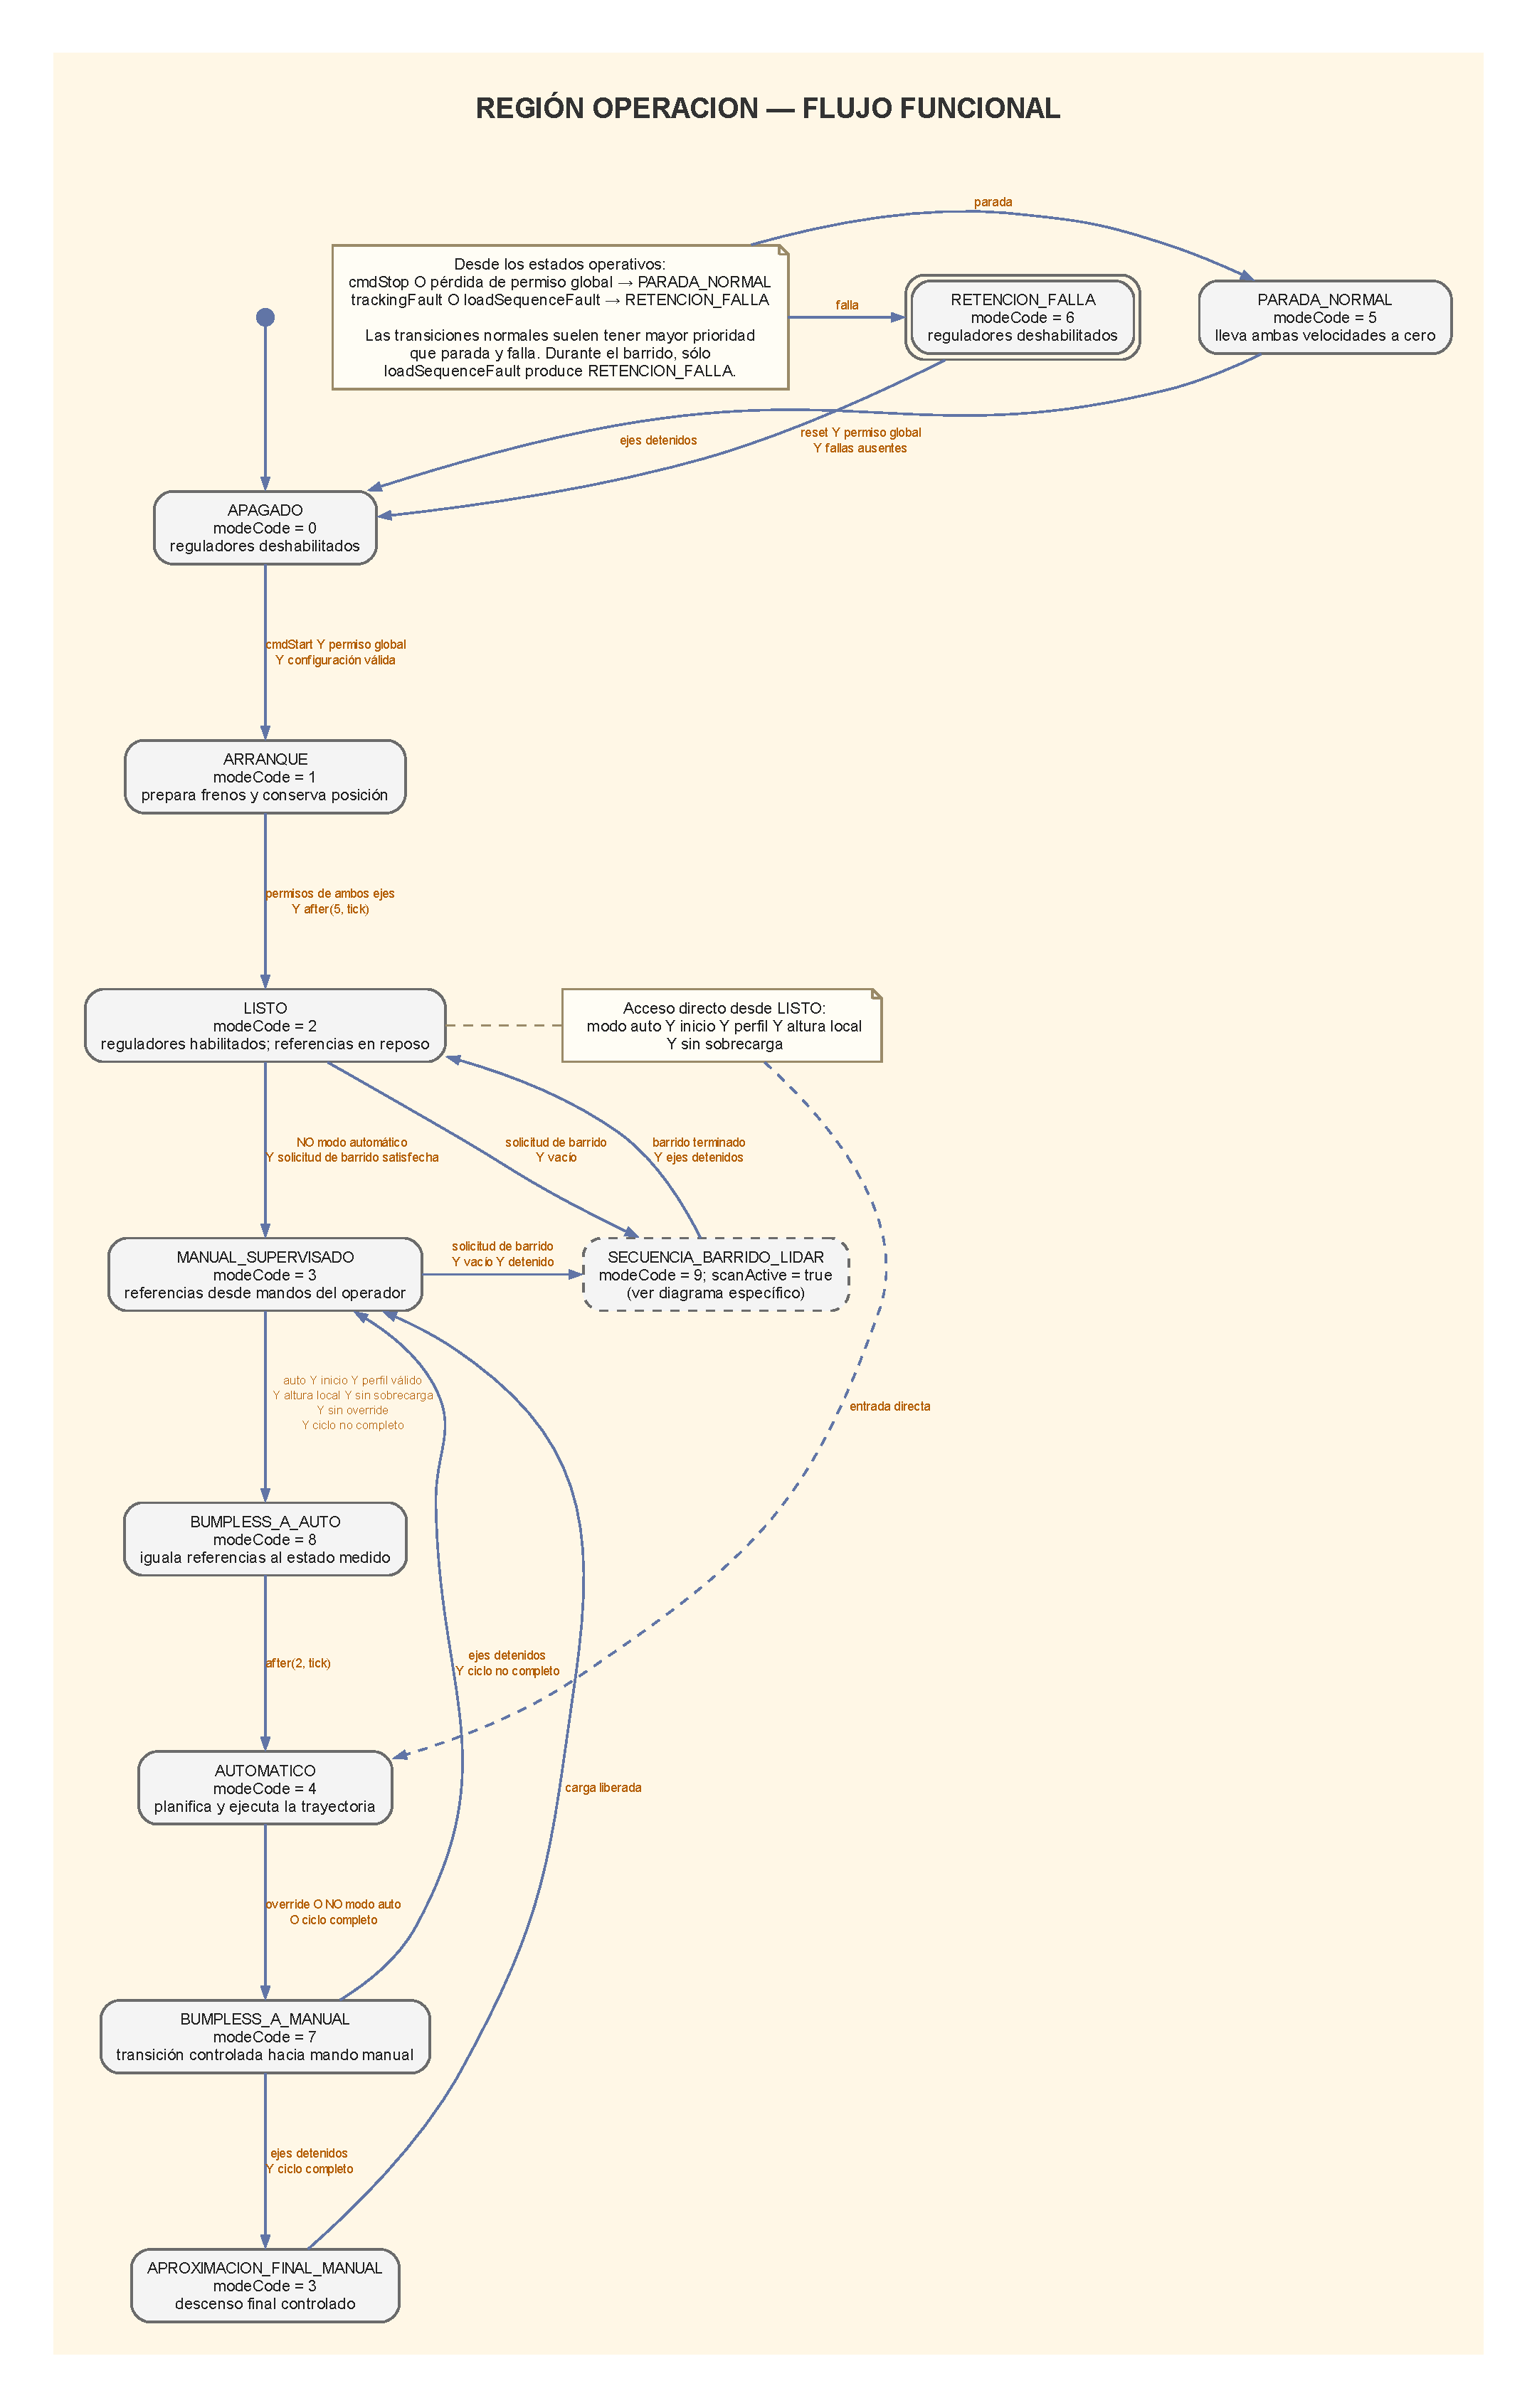
\includegraphics[height=0.82\textheight,keepaspectratio]{diagramas_automatas_revision/02_operacion_supervisor.pdf}
    \caption{Flujo funcional de la región \texttt{OPERACION}, incluyendo arranque, selección de modo, transferencias, barrido, parada y retención de falla.}
\end{figure}


\subsection{Estado MANUAL SUPERVISADO}
En \texttt{MANUAL\_SUPERVISADO} el código de modo es tres. Los \textit{joysticks} se convierten en velocidades con una zona muerta de $0.05$. La velocidad horizontal se limita a $4~\mathrm{m/s}$. La velocidad vertical depende del estado de carga y de la masa estimada.

Si existe sobrecarga, se anula el movimiento horizontal y solamente se permite descender con un máximo de $0.15~\mathrm{m/s}$. Los finales de carrera normales inhiben cualquier orden que intente continuar hacia afuera del recorrido. Las referencias de posición se actualizan integrando una muestra de la velocidad limitada.

Desde \texttt{MANUAL\_SUPERVISADO}, el cambio a automático exige solicitud de modo automático, orden de inicio, perfil válido, \texttt{autoEntryHeightOK}, ausencia de sobrecarga, ausencia de intervención del operador y que no exista un ciclo automático ya completado. No se exige \texttt{loadedState}, por lo que la secuencia admite traslado cargado y retorno vacío. La altura mínima se evalúa en la posición actual a partir de la envolvente local; no se utiliza \texttt{clearanceOK} como guarda.


\subsection{Transferencia a automático}
El estado \texttt{BUMPLESS\_A\_AUTO} se utiliza únicamente para la transferencia desde manual y emplea el código de modo ocho. Las referencias se igualan al estado medido:
\begin{align}
x^*&=x_t,&v_x^*&=v_t,&a_x^*&=a_t,\\
y^*&=y_h,&v_y^*&=v_h,&a_y^*&=a_h.
\end{align}
Después de dos ciclos se ingresa al estado compuesto \texttt{AUTOMATICO}. Esta espera permite que los reguladores reciban una muestra coherente y evita un cambio discontinuo de torque. Existe, además, la transición directa antes mencionada desde \texttt{LISTO}; por lo tanto, no toda entrada al automático atraviesa este estado de transferencia.

Si durante la transferencia aparece una orden de parada, se va a parada normal. Si aparece una falla de seguimiento o de carga, se ingresa a retención de falla.


\subsection{Subestados automáticos}
El estado \texttt{AUTOMATICO} memoriza \texttt{autoTargetX} en \texttt{autoTargetXLatched} y calcula la superficie y la altura de aproximación con \texttt{safetyEnvelopeProfile}. En cada activación posterior, \texttt{INTERLOCKS} vuelve a evaluar el objetivo vertical mediante \texttt{calcularObjetivoSeguro}; \texttt{automaticTargetY} reproduce \texttt{autoApproachTargetY}. La altura objetivo sigue la ecuación \eqref{eq:objetivo_local_vigente} y ya no se reemplaza por el máximo entre destino y línea global.

Los subestados implementados son:
\begin{itemize}
    \item \texttt{PLANIFICAR}: utiliza el código de modo cuatro, reinicia \texttt{craneTrajectoryGenerator} y obtiene el primer punto del plan coordinado.
    \item \texttt{EJECUTAR}: evalúa la trayectoria en cada ciclo, administra la habilitación anti-sway y aplica el cierre adicional de posición vertical.
    \item \texttt{MANTENER\_OBJETIVO}: fija las referencias finales y declara completo el ciclo automático.
\end{itemize}
La transición a \texttt{MANTENER\_OBJETIVO} exige solamente un error horizontal menor que $0.08~\mathrm{m}$ y un error vertical menor que $0.15~\mathrm{m}$. El generador inicia izaje y traslación simultáneamente y, si la envolvente no despeja el perfil, aumenta la duración horizontal. Utiliza el perfil dilatado, la altura del contenedor cuando hay carga, el estiramiento estimado del cable y un margen vertical de $2.59~\mathrm{m}$. La cota alta de cruce conserva además el máximo del perfil más $5.18~\mathrm{m}$. Cuando el descenso final empieza al concluir la traslación, el generador espera las condiciones de posición, velocidad y balanceo descritas en la sección de anti-sway. Durante ejecución se mantiene \texttt{swayControlEnable} según \texttt{swayControlSelect}.

\begin{figure}[!htbp]
    \centering
    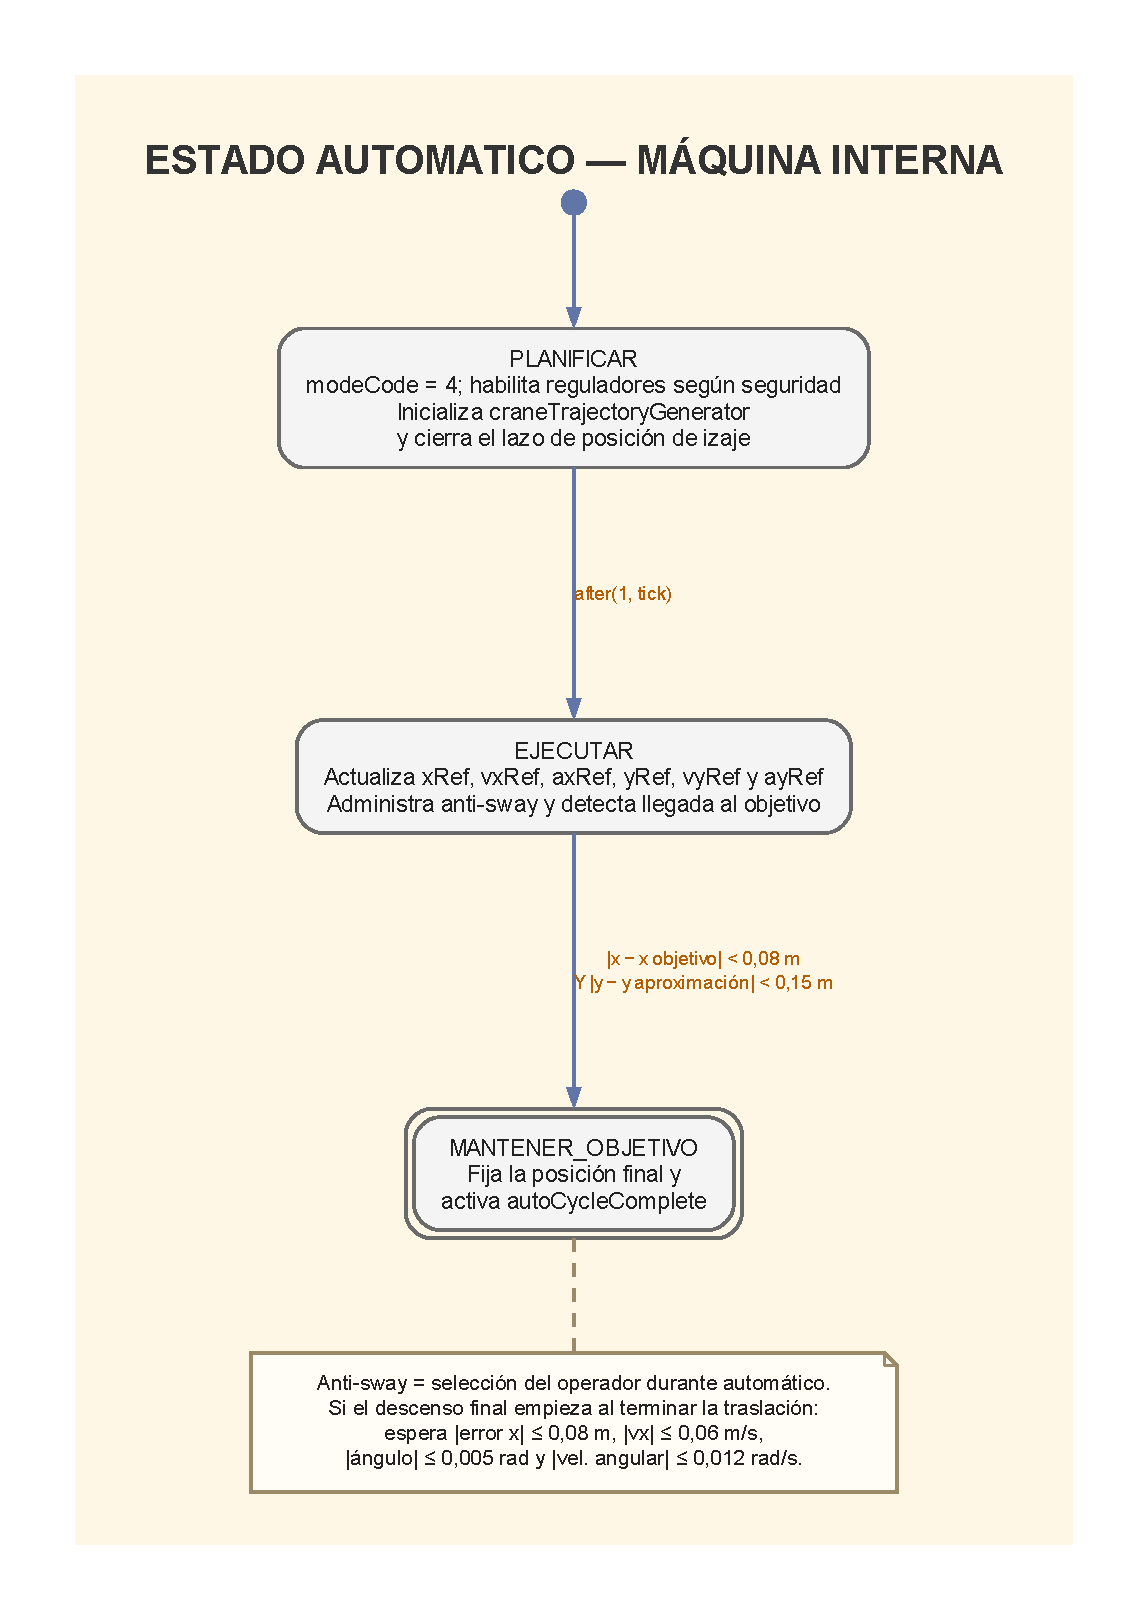
\includegraphics[height=0.75\textheight,keepaspectratio]{diagramas_automatas_revision/03_automatico_interno.pdf}
    \caption{Máquina de estados interna del modo automático y acciones principales de planificación, ejecución y mantenimiento del objetivo.}
\end{figure}


\subsection{Retorno a manual y aproximación final}
El automático finaliza por objetivo alcanzado, intervención del operador o cancelación del modo. Se ingresa a \path{BUMPLESS_A_MANUAL}, donde las referencias se acercan gradualmente al mando manual. Si el ciclo automático no terminó, se retorna a \path{MANUAL_SUPERVISADO}.

Cuando el objetivo fue alcanzado se pasa a \texttt{APROXIMACION\_FINAL\_MANUAL}. La posición horizontal queda fijada y el operador controla el movimiento vertical para realizar el descenso. La función limita el mando a ambos sentidos; no impone por sí sola una prohibición de ascenso. La aceleración vertical queda limitada a $0.05~\mathrm{m/s^2}$ para realizar el apoyo en forma controlada. Una vez liberado el contenedor, el autómata vuelve al modo manual general.


\subsection{Parada normal y retención de falla}
\texttt{PARADA\_NORMAL} representa una detención controlada. Al ingresar se fija el código de modo cinco, se deshabilita el anti-sway y las referencias de velocidad se llevan progresivamente a cero mediante los límites de aceleración establecidos. Los reguladores permanecen disponibles durante esta reducción, por lo que la detención se diferencia de una actuación de emergencia. Una vez alcanzada la condición de reposo, el sistema retorna a \texttt{APAGADO} y requiere una nueva orden de marcha.

\texttt{RETENCION\_FALLA} se utiliza cuando aparece una falla de seguimiento, una falla de la secuencia de carga en los estados que contienen dicha transición. En este estado se deshabilita la continuidad de la maniobra y se conservan los indicadores de diagnóstico. La salida no es automática: exige orden de reinicio, permiso global restablecido y desaparición de las condiciones que originaron la retención. El destino es \texttt{APAGADO}, de modo que el rearme no produce una reanudación espontánea de la trayectoria anterior.

La emergencia se mantiene fuera de estos dos estados. Su intervención corresponde al autómata de seguridad, que actúa sobre permisos y autorizaciones de freno independientemente de la secuencia productiva.


\subsection{Estados del barrido LIDAR}
La secuencia de barrido utiliza cuatro estados. \texttt{PREPARAR\_ESCANEO\_LIDAR} inicializa las 33 alturas en $-20~\mathrm{m}$, pone en cero los contadores de muestras, marca el perfil como no válido y eleva el \textit{spreader} hasta aproximadamente $39.7~\mathrm{m}$. En esta inicialización se carga de manera explícita el \textit{slot} 33 con altura cero y una muestra válida. En consecuencia, la validación posterior exige muestras efectivas en los restantes \textit{slots}, pero el último queda considerado cubierto desde el inicio.

\texttt{IR\_EXTREMO\_DERECHO} mueve el carro hasta el límite normal o hasta $x\geq48.40~\mathrm{m}$ con velocidad pequeña. \texttt{BARRIDO\_LIDAR\_IZQUIERDA} registra el máximo medido en cada \textit{slot} durante el retorno hasta el límite izquierdo o hasta $x\leq-24.50~\mathrm{m}$. \texttt{FINALIZAR\_ESCANEO\_LIDAR} detiene el carro, marca la secuencia como completa y llama a \texttt{verificarCoberturaPerfil}, que exige un contador mayor o igual que uno para cada posición.

El barrido no puede iniciarse con carga. Durante los cuatro estados se atiende la orden de parada y la pérdida del permiso global. Las transiciones específicas hacia \texttt{RETENCION\_FALLA} comprueban \texttt{loadSequenceFault}, pero no incluyen \texttt{trackingFault}.

\begin{figure}[!htbp]
    \centering
    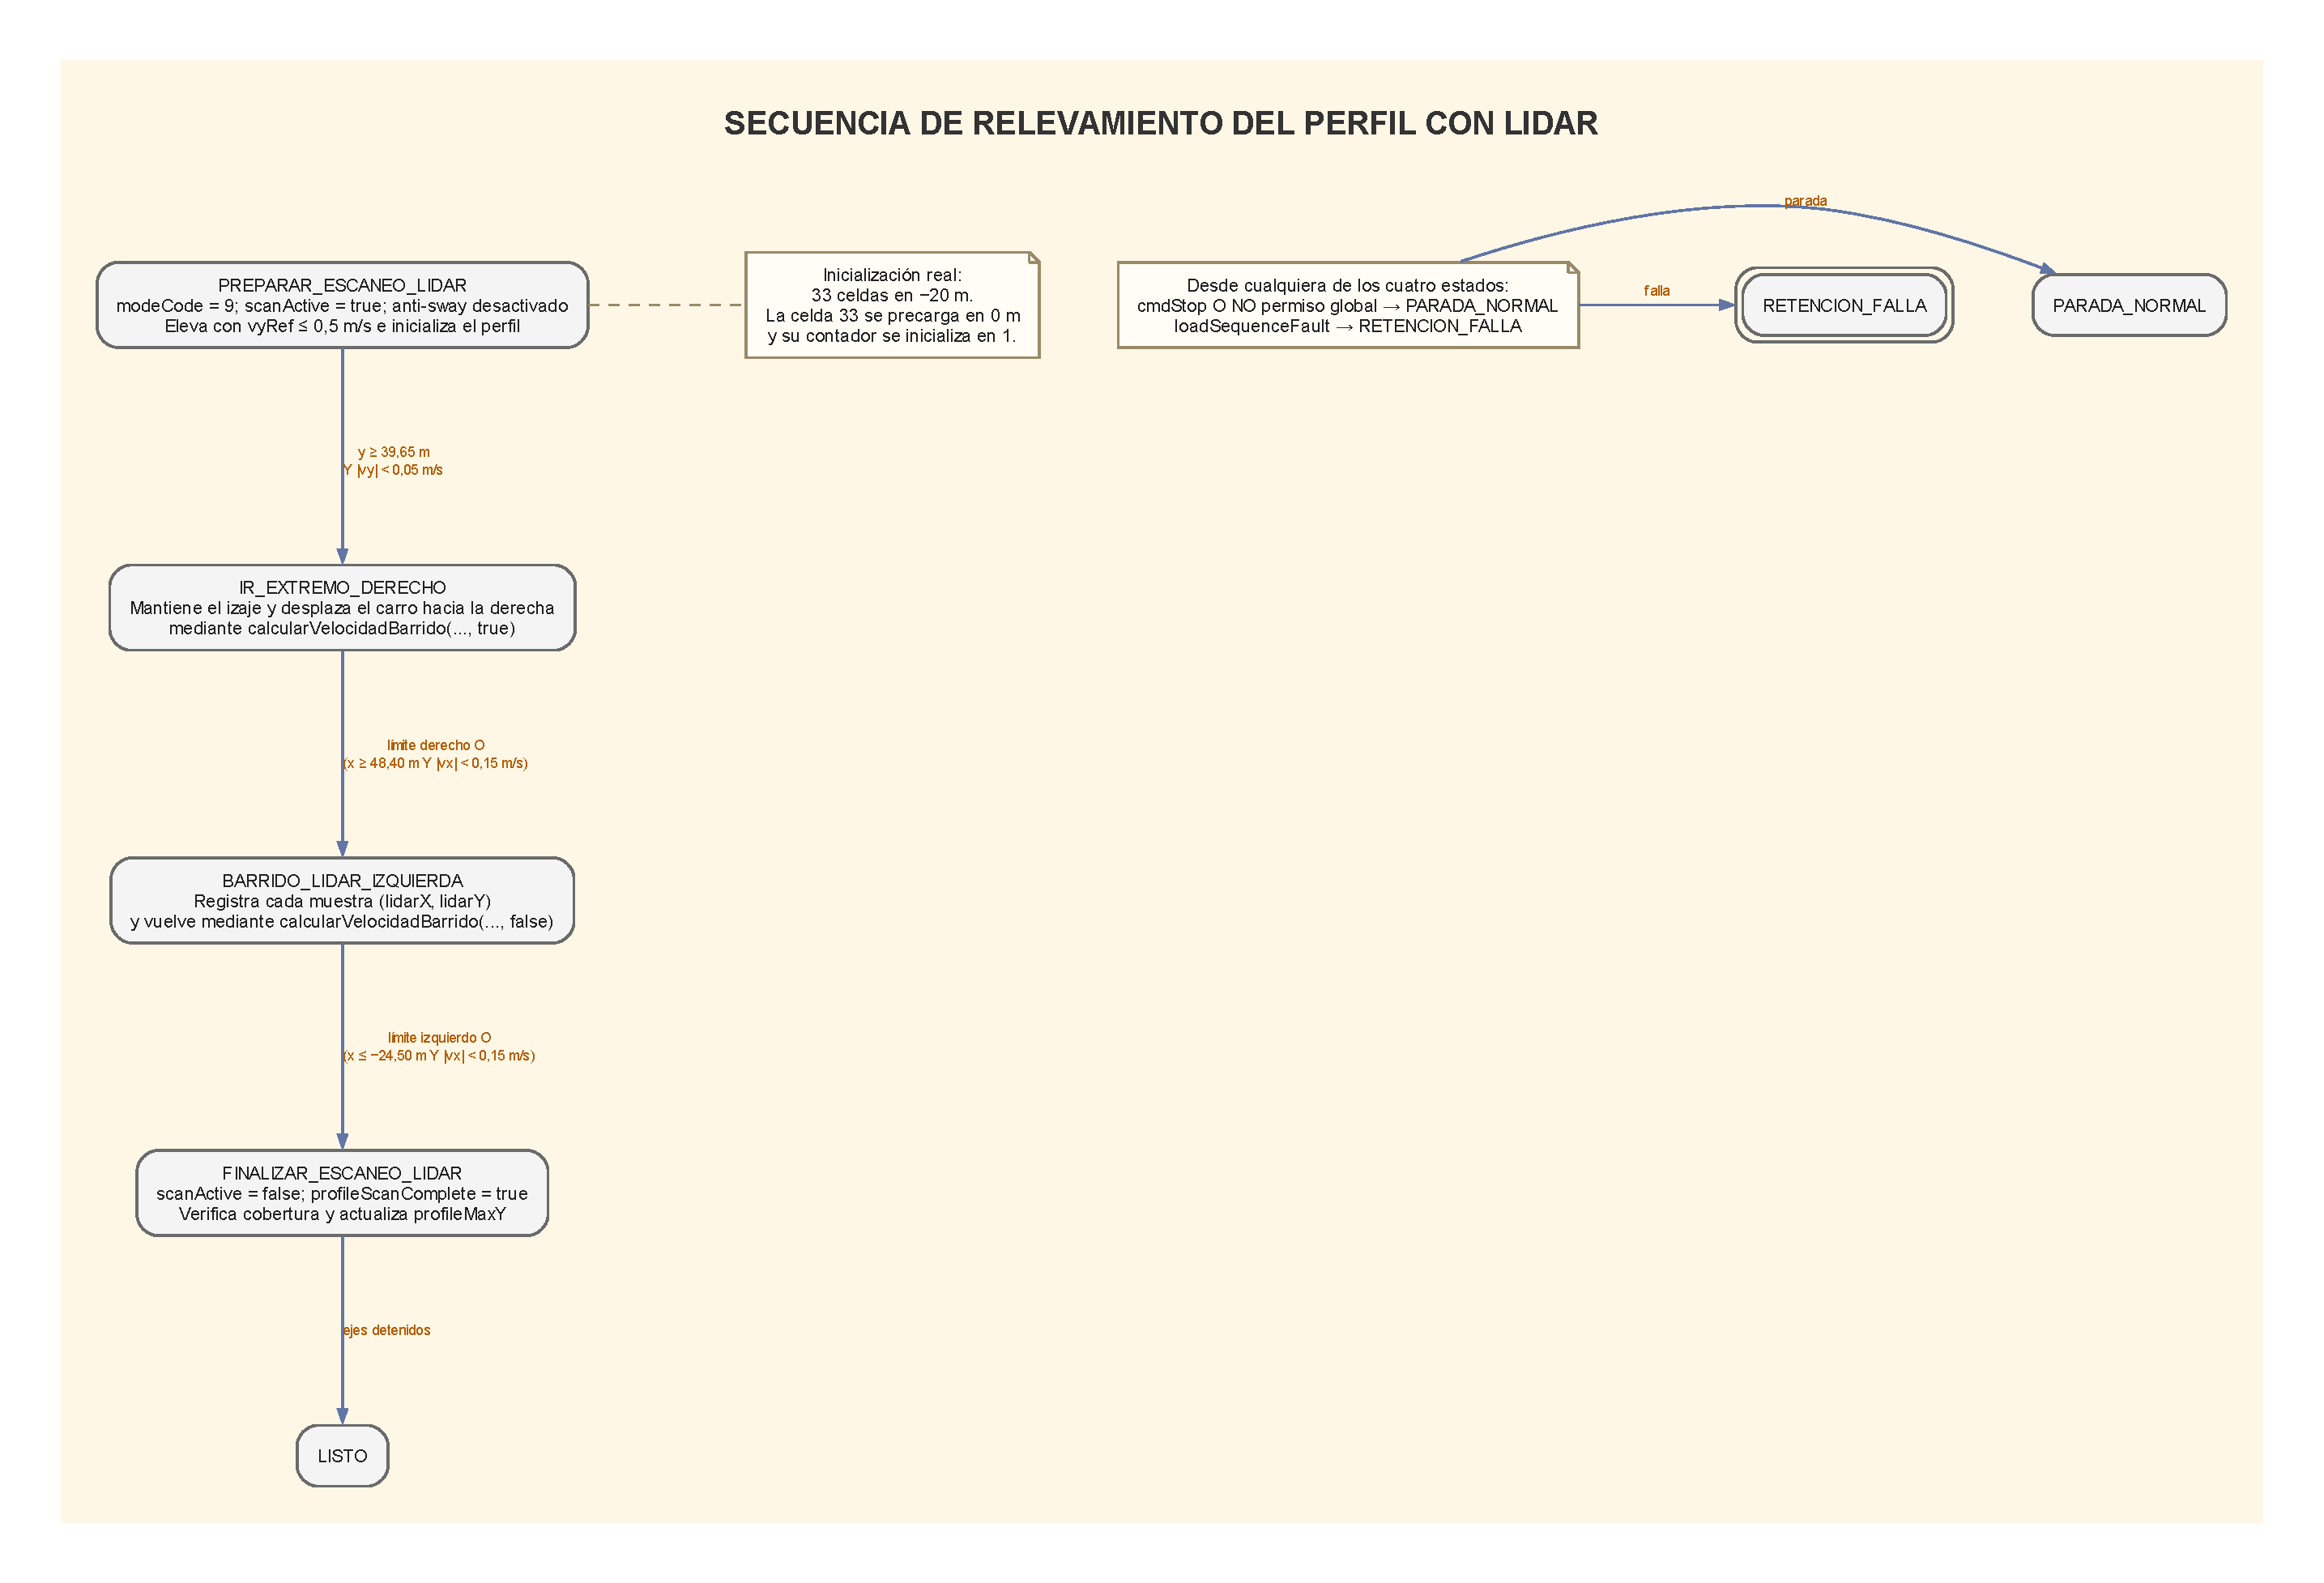
\includegraphics[width=0.98\textwidth,height=0.72\textheight,keepaspectratio]{diagramas_automatas_revision/04_barrido_lidar.pdf}
    \caption{Secuencia automática de relevamiento del perfil mediante LiDAR, con acciones, condiciones de avance y salidas por parada o falla.}
\end{figure}


\subsection{Secuencia de toma y estabilización}
La región de carga comienza en \texttt{VACIO}. Ante una solicitud de cierre, contacto en los cuatro apoyos y permiso de izaje, pasa a \texttt{ESPERAR\_ESTABILIZACION\_SPREADER}. Se exige durante un segundo
\begin{equation}
|\theta_l|\leq0.010~\mathrm{rad},\qquad |\dot\theta_l|\leq0.020~\mathrm{rad/s}.
\end{equation}
Luego se ingresa a \path{CERRANDO_TWISTLOCKS}. Si la confirmación no aparece antes de 100 ciclos se declara \path{FALLA_TWISTLOCK}. Al confirmarse el cierre se ingresa a \path{DESPEGUE_SUAVE}, donde se activa \texttt{loadedState} y \texttt{pickupModeActive}, sin habilitar todavía la estimación de masa.

Mientras el contenedor continúa apoyado y no se completó una segunda comprobación de estabilidad posterior al cierre, \texttt{aplicarRetencionToma} fuerza a cero las referencias manuales horizontal y vertical. El estado \path{DESPEGUE_SUAVE} no contiene una rampa ni un límite de velocidad propios; una vez liberada esta retención se aplican los límites generales del mando manual cargado. Antes de completar el pesaje, \texttt{totalSuspendedMass} conserva el valor inicial de $15000~\mathrm{kg}$ y el cálculo manual puede admitir hasta $3~\mathrm{m/s}$.


\subsection{Pesaje y sobrecarga}
Cuando el cable deja de estar flojo, $|v_h|<0.20~\mathrm{m/s}$ y $|a_h|<0.05~\mathrm{m/s^2}$, se ingresa a \texttt{PESAJE}. Durante 25 ciclos se acumulan muestras de masa estimada. El promedio reduce el efecto de oscilaciones de tensión.

Si la masa estimada del contenedor no supera $50000~\mathrm{kg}$ se pasa a \texttt{CARGADO}. Si supera ese límite se pasa a \texttt{SOBRECARGA}. En sobrecarga no se permite el traslado y solamente puede ordenarse una descarga controlada.

La apertura de \textit{twistlocks} se permite con contacto. El estado \texttt{ABRIENDO\_TWISTLOCKS} espera la confirmación de apertura y retorna a \texttt{VACIO}. También dispone de un tiempo máximo de 100 ciclos.


\subsection{Indexación de estados de carga}
\begin{table}[!htbp]
\centering
\caption{Índice funcional de la región de carga.}
\begin{tabular}{C{1.2cm} L{5cm} L{7.2cm}}
\toprule
Índice & Estado & Acción principal\\
\midrule
C0 & \texttt{VACIO} & Reinicia masa, carga y comandos de cierre.\\
C1 & \path{ESPERAR_ESTABILIZACION_SPREADER} & Verifica ángulo y velocidad angular.\\
C2 & \texttt{CERRANDO\_TWISTLOCKS} & Comanda cierre y temporiza confirmación.\\
C3 & \texttt{DESPEGUE\_SUAVE} & Declara carga tomada y retiene el mando hasta la segunda estabilidad; no impone una velocidad propia.\\
C4 & \texttt{PESAJE} & Promedia la masa estimada durante 25 ciclos.\\
C5 & \texttt{CARGADO} & Habilita traslado normal.\\
C6 & \texttt{SOBRECARGA} & Inhibe traslado y limita el descenso.\\
C7 & \texttt{ABRIENDO\_TWISTLOCKS} & Comanda apertura y espera realimentación.\\
C8 & \texttt{FALLA\_TWISTLOCK} & Retiene comandos hasta reinicio seguro.\\
\bottomrule
\end{tabular}
\end{table}

\begin{figure}[!htbp]
    \centering
    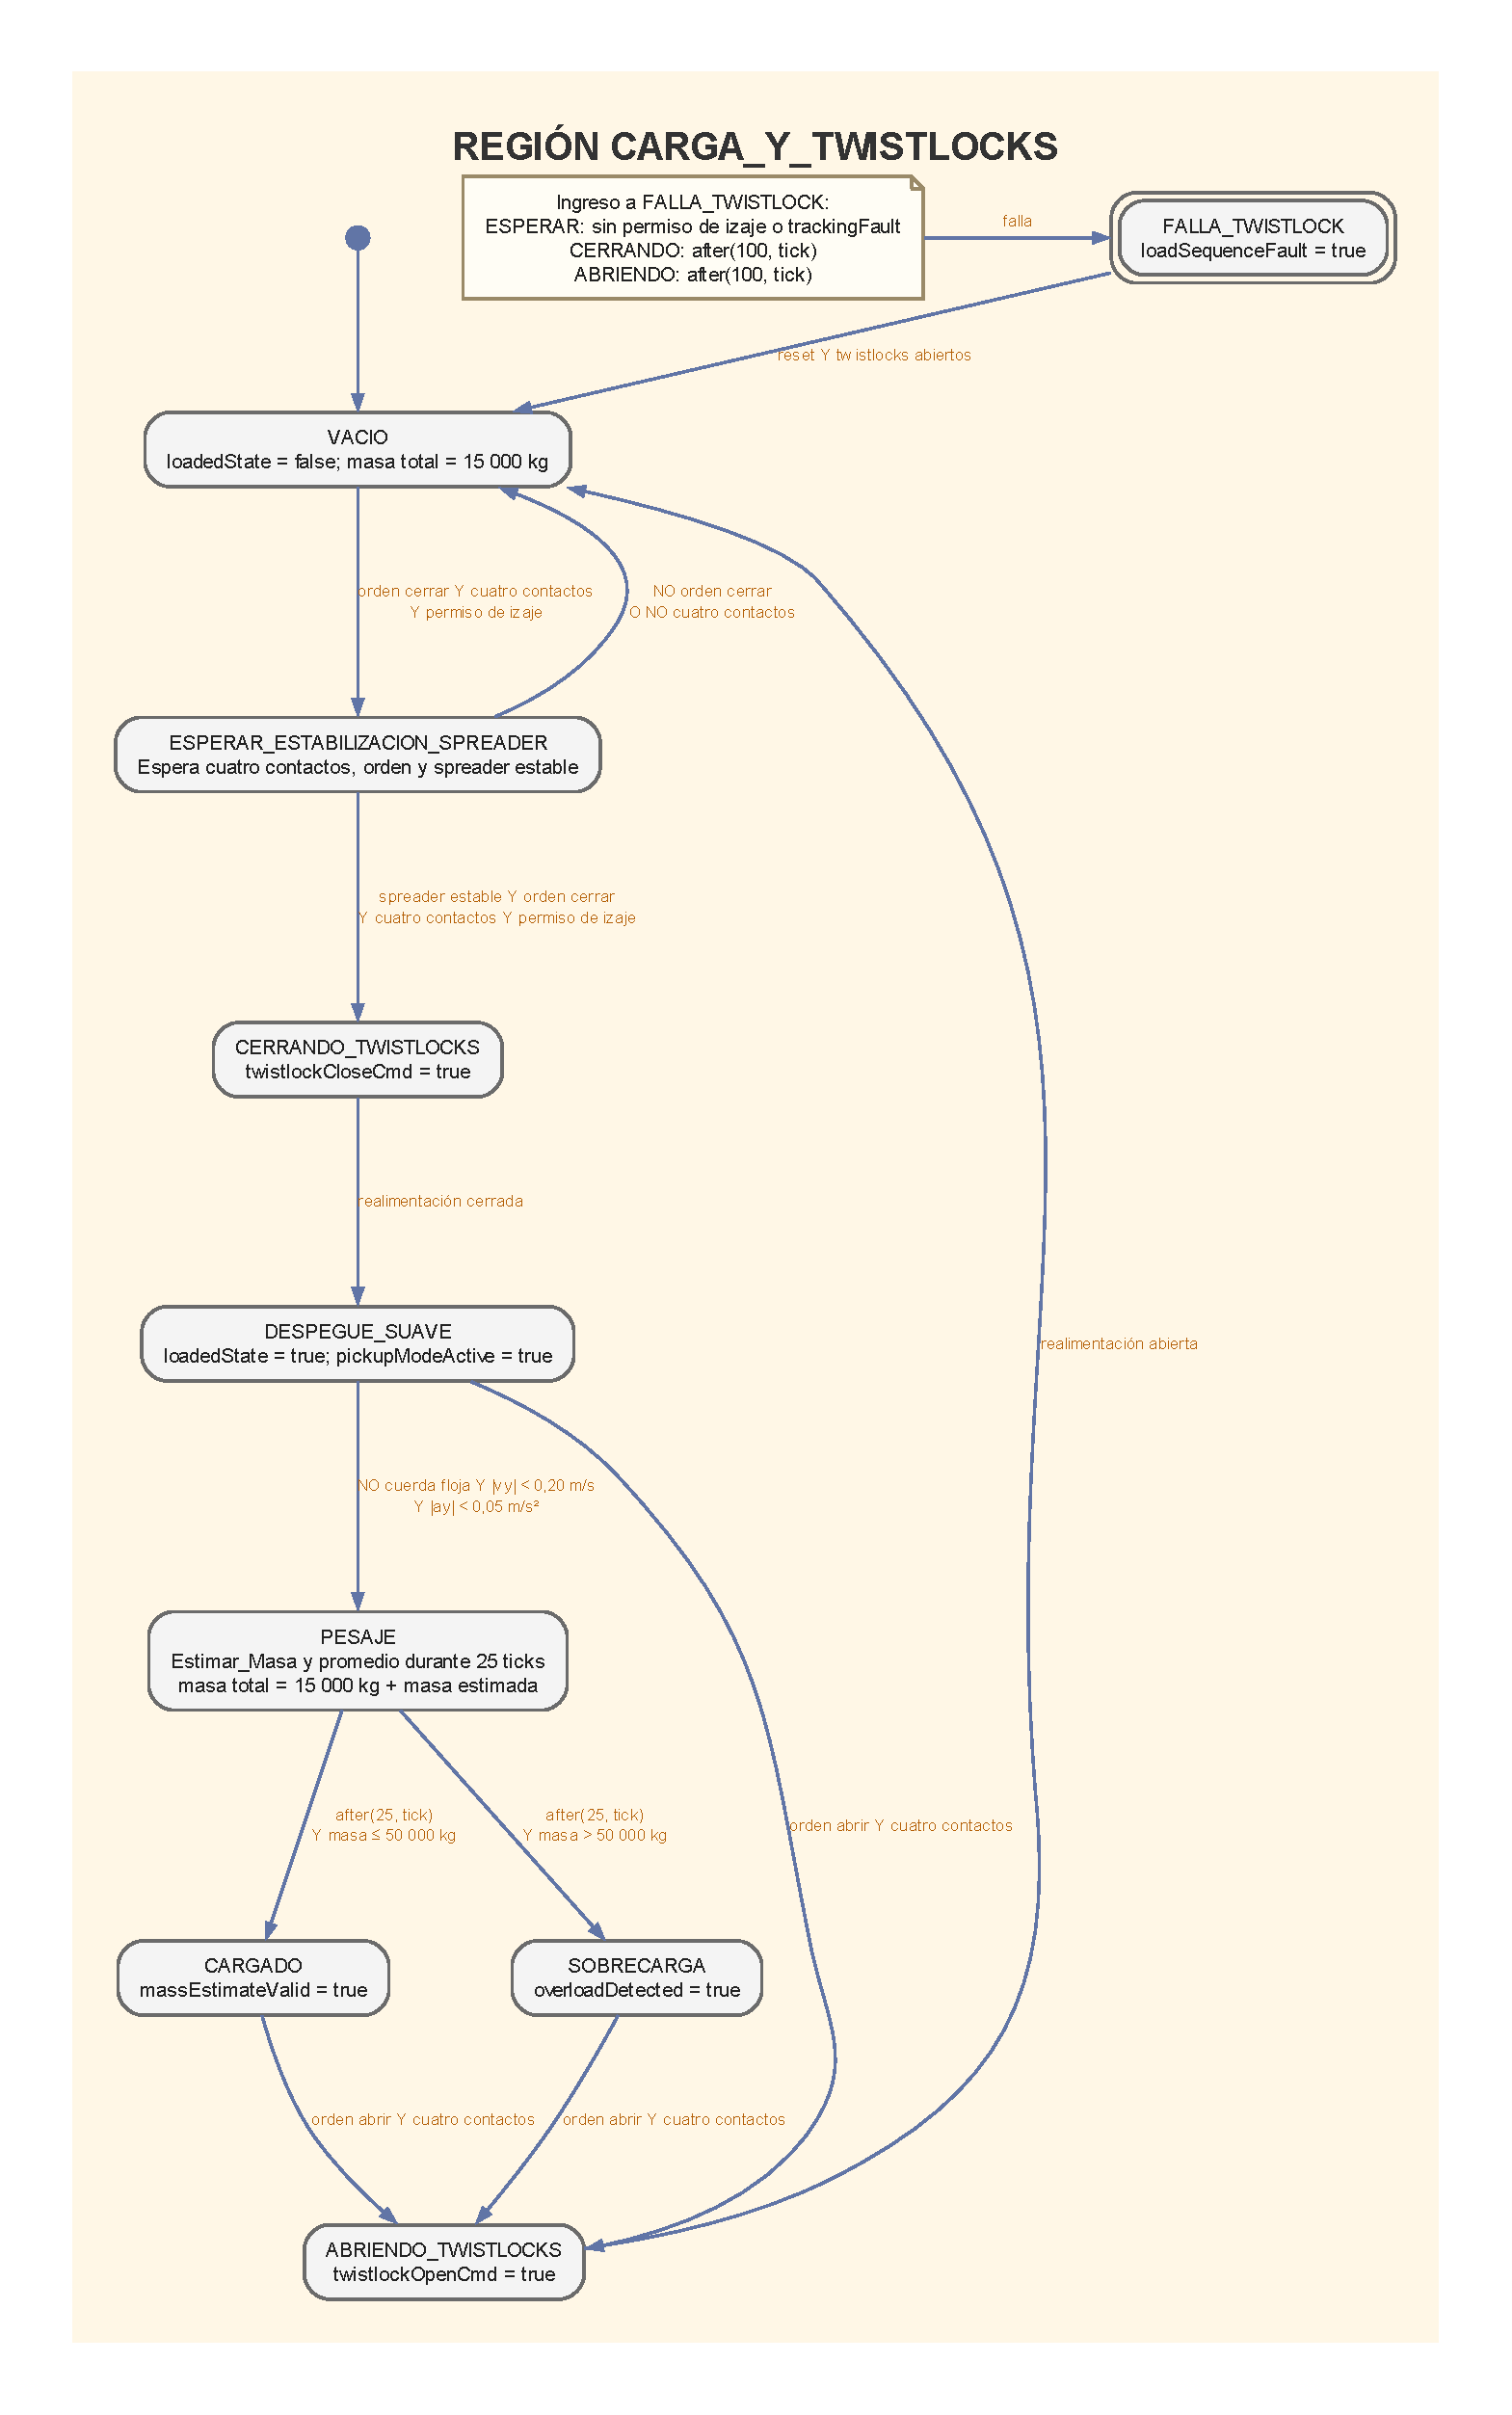
\includegraphics[height=0.82\textheight,keepaspectratio]{diagramas_automatas_revision/05_carga_twistlocks.pdf}
    \caption{Máquina de estados completa de la región \texttt{CARGA\_Y\_TWISTLOCKS}, desde la toma hasta la liberación o retención por falla.}
\end{figure}


\subsection{Secuencia del freno de izaje}
La región \texttt{FRENO\_IZAJE} posee cuatro estados:
\begin{itemize}
    \item H0 -- \texttt{HB\_APLICADO}: freno cerrado.
    \item H1 -- \texttt{HB\_PRUEBA\_TORQUE}: el regulador establece torque con freno aplicado.
    \item H2 -- \texttt{HB\_ABIERTO}: freno liberado durante el movimiento.
    \item H3 -- \texttt{HB\_APLICANDO}: mantiene apertura hasta que velocidad y error son pequeños.
\end{itemize}
Desde H1 se vuelve a H0 si no se demuestra torque antes de 50 ciclos. Desde H2 se pasa a H3 si falta habilitación o permiso de izaje; la ausencia de demanda sólo provoca esta transición cuando \texttt{modeCode} es distinto de cuatro. Así se mantiene el freno operativo abierto durante el automático aun si momentáneamente la referencia de velocidad y el error son pequeños. La apertura solamente se produce con \path{torqueProvenHoist}. Al terminar el movimiento, el freno se aplica cuando $|v_h|<0.03~\mathrm{m/s}$ y el error vertical es menor o igual que $0.05~\mathrm{m}$.


\subsection{Secuencia del freno del carro}
La región \texttt{FRENO\_CARRO} reproduce la misma filosofía:
\begin{itemize}
    \item T0 -- \texttt{TB\_APLICADO}.
    \item T1 -- \texttt{TB\_PRUEBA\_TORQUE}.
    \item T2 -- \texttt{TB\_ABIERTO}.
    \item T3 -- \texttt{TB\_APLICANDO}.
\end{itemize}
La prueba comienza si el regulador está habilitado, existe una referencia de movimiento y el permiso de seguridad del carro está activo. La aplicación final exige $|v_t|<0.03~\mathrm{m/s}$ y error de posición menor o igual que $0.03~\mathrm{m}$.

Estas máquinas impiden liberar un freno por la sola presencia de una orden de movimiento. La confirmación de torque proporciona una condición adicional antes de dejar el eje libre.

La indexación consolidada de ambas regiones se presenta en la \cref{tab:indices_frenos}. La letra identifica el eje y permite conservar el mismo número para estados de función equivalente.

\begin{table}[!htbp]
\centering
\caption{Índice y acciones de los estados de freno.}\label{tab:indices_frenos}
\begin{tabular}{C{1.1cm} L{4.3cm} L{8.0cm}}
\toprule
Índice & Estado & Acción documentada\\
\midrule
H0 & \texttt{HB\_APLICADO} & Mantiene aplicado el freno de izaje.\\
H1 & \texttt{HB\_PRUEBA\_TORQUE} & Solicita torque y espera su comprobación.\\
H2 & \texttt{HB\_ABIERTO} & Autoriza la apertura durante el movimiento vertical.\\
H3 & \texttt{HB\_APLICANDO} & Espera reposo y completa la aplicación del freno.\\
T0 & \texttt{TB\_APLICADO} & Mantiene aplicado el freno del carro.\\
T1 & \texttt{TB\_PRUEBA\_TORQUE} & Solicita torque y espera su comprobación.\\
T2 & \texttt{TB\_ABIERTO} & Autoriza la apertura durante el movimiento horizontal.\\
T3 & \texttt{TB\_APLICANDO} & Espera reposo y completa la aplicación del freno.\\
\bottomrule
\end{tabular}
\end{table}

\begin{figure}[!htbp]
    \centering
    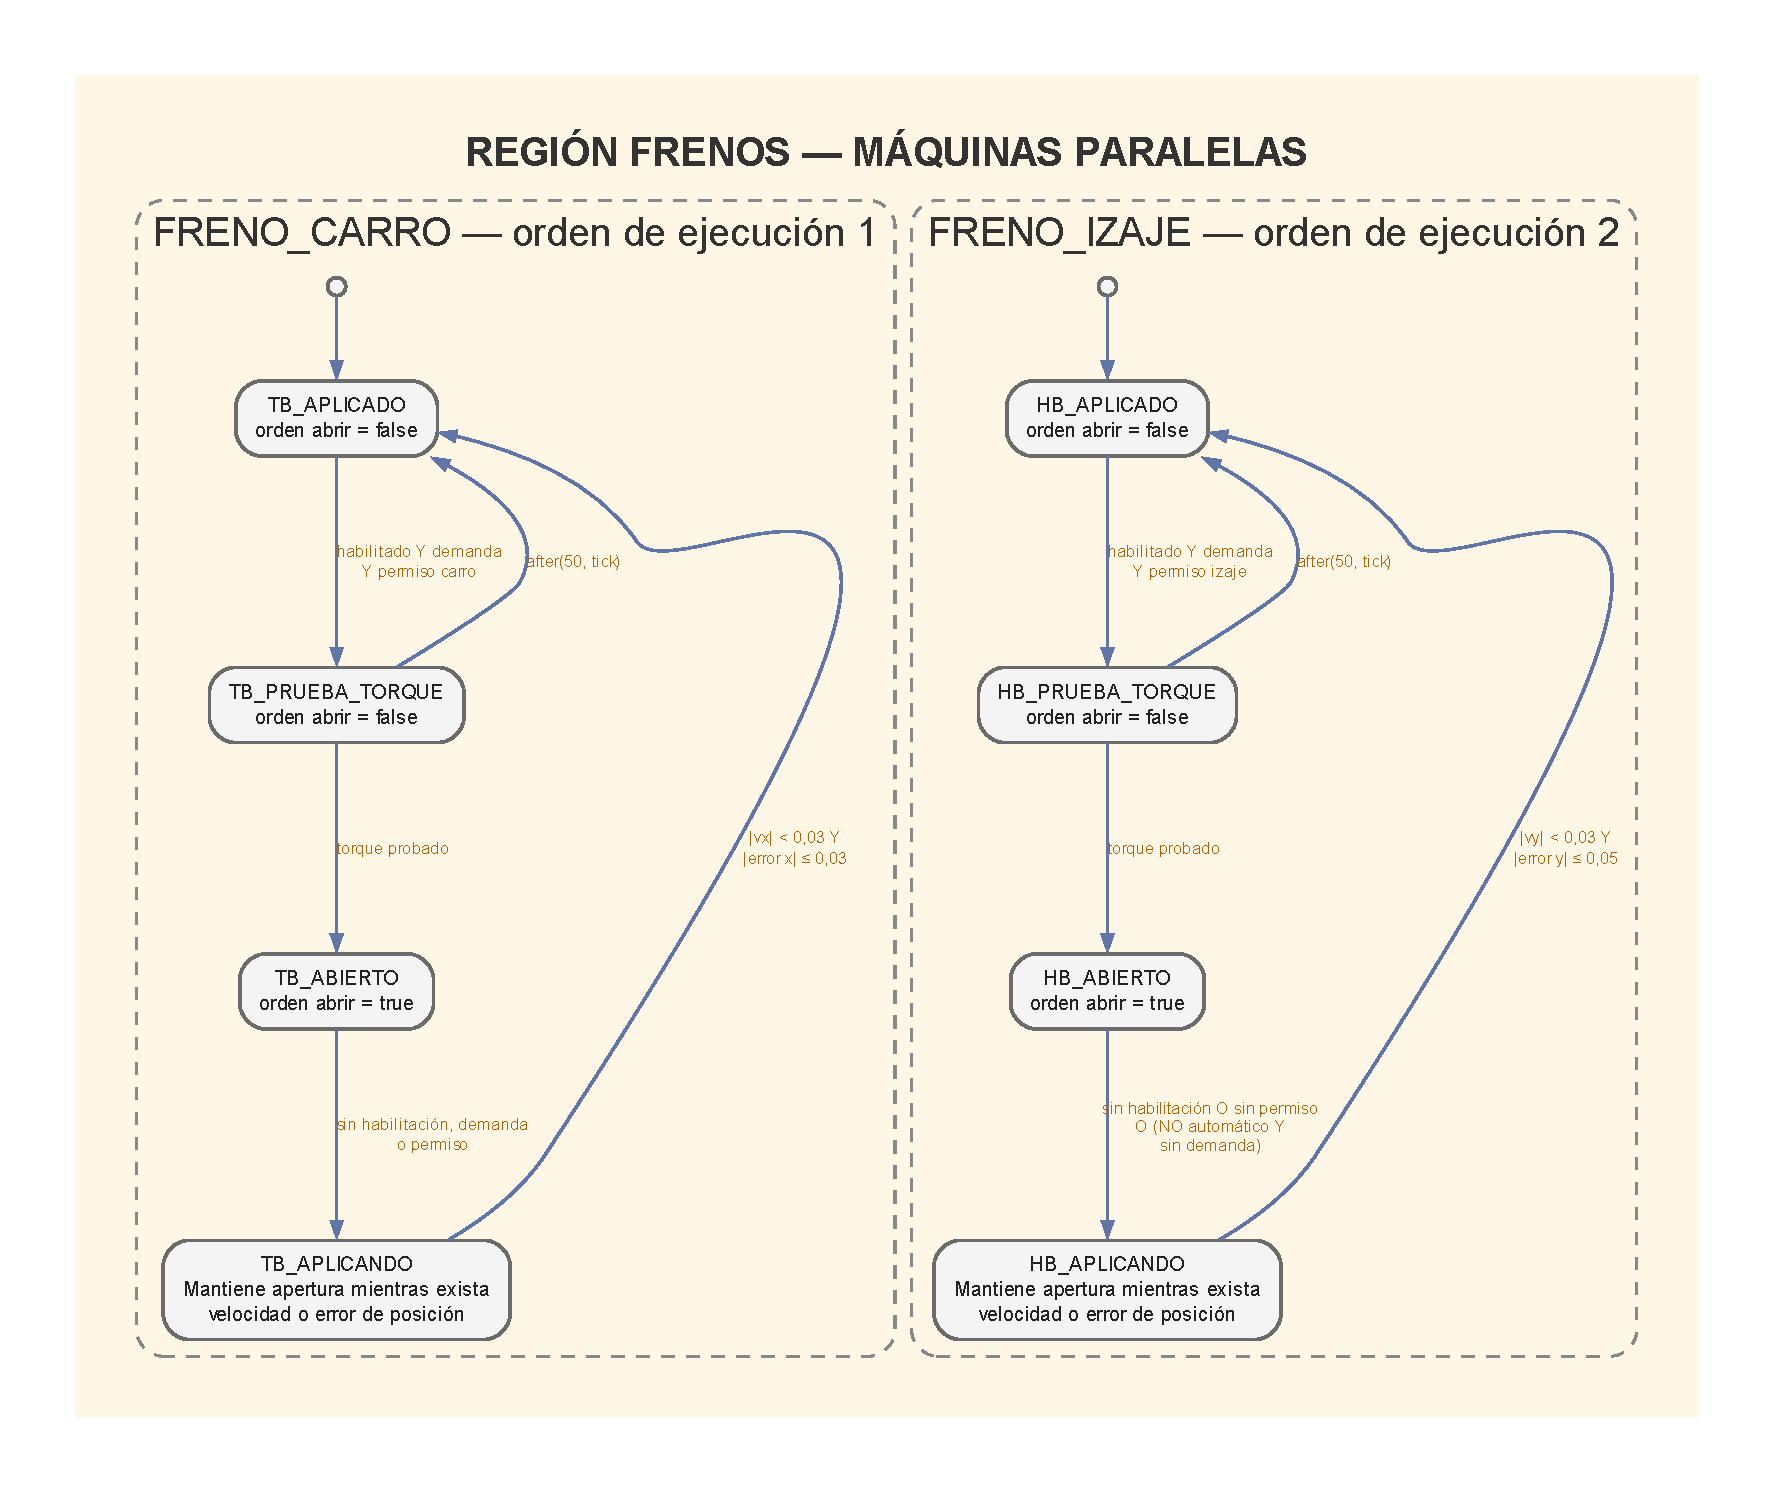
\includegraphics[width=0.98\textwidth,height=0.72\textheight,keepaspectratio]{diagramas_automatas_revision/06_frenos.pdf}
    \caption{Máquinas paralelas de accionamiento de los frenos del carro y del izaje.}
\end{figure}


\subsection{Diagnóstico del supervisor}
La región \texttt{DIAGNOSTICO} contiene \texttt{DIAG\_OK}, \texttt{ALARMA} y \texttt{FALLA}. La sobrecarga produce una alarma recuperable. Una falla de seguimiento, una falla de secuencia de carga o la pérdida del permiso global produce una falla.

Los códigos implementados son:
\begin{itemize}
    \item código de alarma 1: sobrecarga;
    \item código de falla 10: error de seguimiento sostenido;
    \item código de falla 11: falla de secuencia de carga;
    \item código de falla 12: permiso global de seguridad ausente.
\end{itemize}
La falla de seguimiento se activa en los modos cuatro u ocho si $|x^*-x_t|>2.5~\mathrm{m}$ o $|y^*-y_h|>\max(1.00,2|v_h|+0.25)~\mathrm{m}$ se mantiene durante al menos tres segundos. En los demás modos se reinicia el temporizador.

\begin{table}[!htbp]
\centering
\caption{Índice funcional de la región de diagnóstico.}\label{tab:indice_diagnostico}
\begin{tabular}{C{1.2cm} L{3.5cm} L{8.7cm}}
\toprule
Índice & Estado & Función\\
\midrule
D0 & \texttt{DIAG\_OK} & Mantiene códigos de alarma y falla sin condición activa.\\
D1 & \texttt{ALARMA} & Informa sobrecarga recuperable mediante el código de alarma 1.\\
D2 & \texttt{FALLA} & Conserva el código correspondiente a seguimiento, carga o permiso global.\\
\bottomrule
\end{tabular}
\end{table}

\begin{figure}[!htbp]
    \centering
    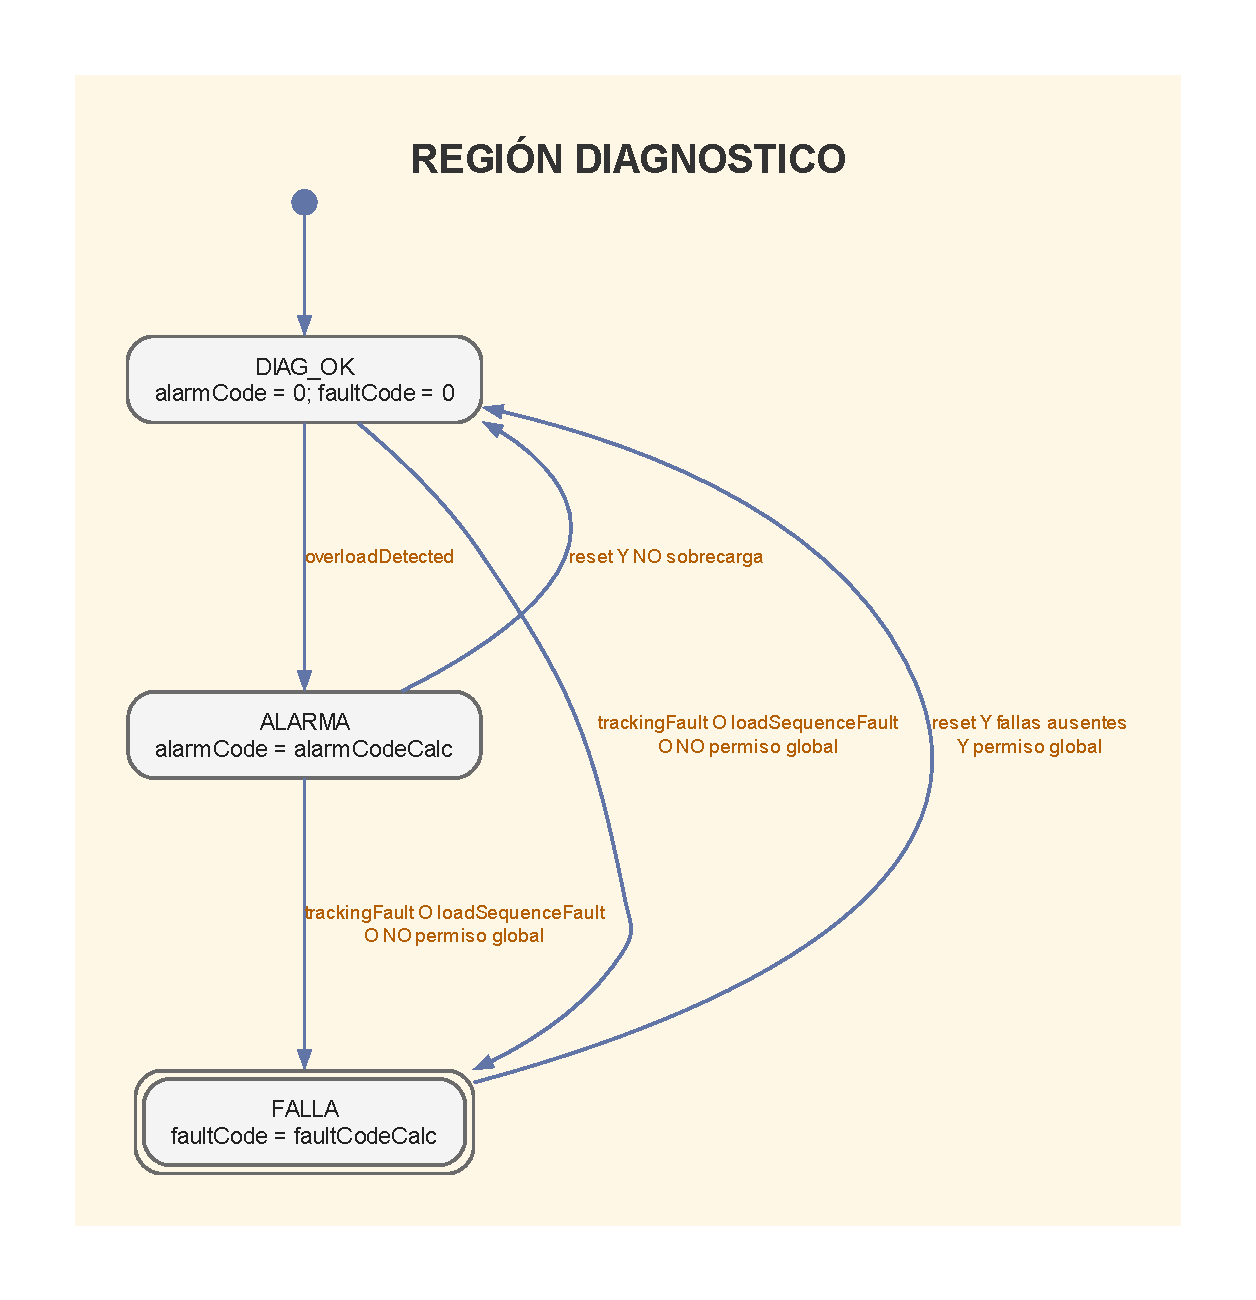
\includegraphics[height=0.68\textheight,keepaspectratio]{diagramas_automatas_revision/07_diagnostico.pdf}
    \caption{Región de diagnóstico del supervisor y condiciones de generación y recuperación de alarmas y fallas.}
\end{figure}


\subsection{Resumen de transiciones prioritarias}
La prioridad efectiva queda determinada por el orden de ejecución de las transiciones salientes de cada estado. En la implementación analizada, las transiciones normales suelen evaluarse antes que las de parada o falla. Por ejemplo, en \texttt{MANUAL\_SUPERVISADO} se evalúan, en este orden, la entrada a automático, la parada normal, la retención de falla y el inicio del barrido. En \texttt{AUTOMATICO} se evalúan primero la salida a \path{BUMPLESS_A_MANUAL}, luego la parada y finalmente la retención de falla. En los estados del barrido también se evalúa primero el avance normal de la secuencia.

Por esta razón, si en una misma activación coinciden una condición normal y \texttt{cmdStop} o una falla, puede ejecutarse primero la transición normal y atenderse la parada o la retención en la activación siguiente. \texttt{cmdStop} o la pérdida del permiso global aparecen como condiciones de \texttt{PARADA\_NORMAL} en los estados operativos, mientras que \texttt{trackingFault} o \texttt{loadSequenceFault} llevan a \texttt{RETENCION\_FALLA} en la mayor parte de la operación. Como se indicó, los estados de barrido sólo incluyen de manera explícita la falla de secuencia de carga.

El reinicio de falla no produce marcha inmediata. Desde \texttt{RETENCION\_FALLA} se vuelve a \texttt{APAGADO} solamente con orden de reinicio, permiso global y ausencia de las fallas que originaron la retención. Luego debe repetirse la secuencia de arranque.

Esta organización mantiene una separación entre detener en forma controlada y actuar por emergencia. La parada normal utiliza los reguladores para llevar las velocidades a cero. La emergencia pertenece al nivel de seguridad y actúa directamente sobre permisos y frenos.

\subsection{Tabla consolidada de transiciones de operación}
La \cref{tab:transiciones_operacion} resume las transiciones que definen el recorrido funcional principal. La prioridad indicada corresponde al orden relativo descrito por el modelo cuando más de una condición puede resultar verdadera en la misma activación.

{\footnotesize
\begin{longtable}{L{3.5cm} L{3.5cm} L{6.4cm} C{1.0cm}}
\caption{Transiciones principales de la región \texttt{OPERACION}.}\label{tab:transiciones_operacion}\\
\toprule
Origen & Destino & Condición funcional resumida & Orden\\
\midrule
\endfirsthead
\toprule
Origen & Destino & Condición funcional resumida & Orden\\
\midrule
\endhead
\texttt{APAGADO} & \texttt{ARRANQUE} & Marcha, permiso global y configuración válida & 1\\
\texttt{ARRANQUE} & \texttt{LISTO} & Cinco ciclos con permisos de ambos ejes & 1\\
\texttt{LISTO} & \texttt{MANUAL\_SUPERVISADO} & Modo manual y solicitud de barrido ausente o satisfecha & 1\\
\texttt{LISTO} & \texttt{AUTOMATICO} & Modo e inicio automático, perfil válido, altura local y sin sobrecarga & 2\\
\texttt{LISTO} & \path{PREPARAR_ESCANEO_LIDAR} & Escaneo pendiente, no completado y conjunto vacío & 5\\
\path{MANUAL_SUPERVISADO} & \path{BUMPLESS_A_AUTO} & Inicio automático, perfil y altura local válidos, sin sobrecarga ni intervención, ciclo no completo & 1\\
\path{MANUAL_SUPERVISADO} & \texttt{PARADA\_NORMAL} & Orden de parada o pérdida de permiso & 2\\
\path{MANUAL_SUPERVISADO} & \texttt{RETENCION\_FALLA} & Falla de seguimiento o de carga & 3\\
\path{BUMPLESS_A_AUTO} & \texttt{AUTOMATICO} & Dos ciclos de inicialización cumplidos & 1\\
\texttt{AUTOMATICO} & \path{BUMPLESS_A_MANUAL} & Objetivo, intervención manual o cancelación & 1\\
\texttt{AUTOMATICO} & \texttt{PARADA\_NORMAL} & Orden de parada o pérdida de permiso & 2\\
\texttt{AUTOMATICO} & \texttt{RETENCION\_FALLA} & Falla de seguimiento o de carga & 3\\
\path{BUMPLESS_A_MANUAL} & \path{APROXIMACION_FINAL_MANUAL} & $|v_t|<0.10$, $|v_h|<0.03$ y ciclo completado & 4\\
\path{BUMPLESS_A_MANUAL} & \path{MANUAL_SUPERVISADO} & $|v_t|<0.10$, $|v_h|<0.03$ y ciclo no completado & 1\\
\path{APROXIMACION_FINAL_MANUAL} & \path{MANUAL_SUPERVISADO} & Contenedor liberado & 1\\
\path{FINALIZAR_ESCANEO_LIDAR} & \texttt{LISTO} & Ejes detenidos; no exige \texttt{profileValid} & 1\\
\texttt{RETENCION\_FALLA} & \texttt{APAGADO} & Reinicio, permiso global y causas eliminadas & 1\\
\bottomrule
\end{longtable}
}

\subsection{Particularidades de la implementación analizada}
La descripción precedente reproduce la lógica existente y no supone cambios sobre el modelo. Para evitar interpretar como requisitos generales algunas decisiones específicas de esta implementación, se reúnen a continuación sus particularidades más relevantes:
\begin{itemize}
    \item existe una entrada directa desde \texttt{LISTO} hacia \texttt{AUTOMATICO}, sin atravesar \path{BUMPLESS_A_AUTO};
    \item el automático exige altura local suficiente mediante \texttt{autoEntryHeightOK}; la línea global y \texttt{clearanceOK} no son guardas de entrada;
    \item \path{DESPEGUE_SUAVE} realiza la retención de estabilidad, pero no incorpora una rampa de velocidad propia;
    \item el \textit{slot} 33 del perfil se inicializa con una muestra válida antes del barrido;
    \item los estados del barrido contemplan explícitamente \texttt{loadSequenceFault}, pero no \texttt{trackingFault};
    \item el anti-sway sigue la selección del operador durante el automático; no existe la antigua deshabilitación por velocidad productiva;
    \item el descenso al final de la traslación espera posición, velocidad y estabilidad angular dentro del generador, aunque el fin del chart se decide mediante tolerancias de posición;
    \item ante coincidencia de condiciones, el orden de las transiciones puede hacer que un avance normal se evalúe antes que una parada o falla.
\end{itemize}
Estas observaciones son necesarias para que las tablas, los diagramas y una eventual reproducción externa del autómata mantengan correspondencia con el Stateflow estudiado.



\subsection{Implementación manual del supervisor en CODESYS}
El supervisor se distribuye en 16 programas SFC. Las salidas y los cálculos numéricos se implementan en ST: \path{PRG_PREPROCESO} acondiciona entradas y construye las banderas comunes, mientras \path{PRG_ACCIONES_Y_SALIDAS} consulta los pasos activos, calcula referencias y aplica interbloqueos finales. Las variables compartidas pertenecen a \path{GVL_GRUA}. Un paso activo se consulta mediante \texttt{Paso.x}; su permanencia se consulta mediante \texttt{Paso.t}. Los SFC exportados no contienen bloques de acción IEC: sus efectos se materializan en los programas ST de la tarea.

\path{MainTask_20ms} ejecuta una lista fija de llamadas cada $20~\mathrm{ms}$. Primero se procesa el enlace OPC UA y se ejecuta seguridad. Luego se ejecutan preprocesamiento, cuerda floja, contenedor paralelo, ciclo, modos, barrido, automático, carga, sobrecarga, fallas de carga, frenos y diagnóstico. El programa de acciones y salidas se llama al final. Por tanto, el orden entre POUs reemplaza parte del orden entre regiones paralelas de Stateflow; no debe suponerse que ambas organizaciones tienen idéntica semántica de ejecución.

\path{SFC_SUPERVISOR_PARALELO} contiene un paso inicial, una divergencia simultánea hacia cinco pasos de región y una convergencia hacia \texttt{DETENIDO}. Su retorno requiere reinicio y permiso global. Estos pasos expresan la organización concurrente; no invocan las secuencias subordinadas como acciones. Las secuencias se ejecutan porque la tarea las llama por separado. En los gráficos, el rectángulo doble identifica el paso inicial, la barra corta identifica una transición, la barra doble indica paralelismo y el salto identifica el destino de retorno.

\begin{figure}[!htbp]
\centering
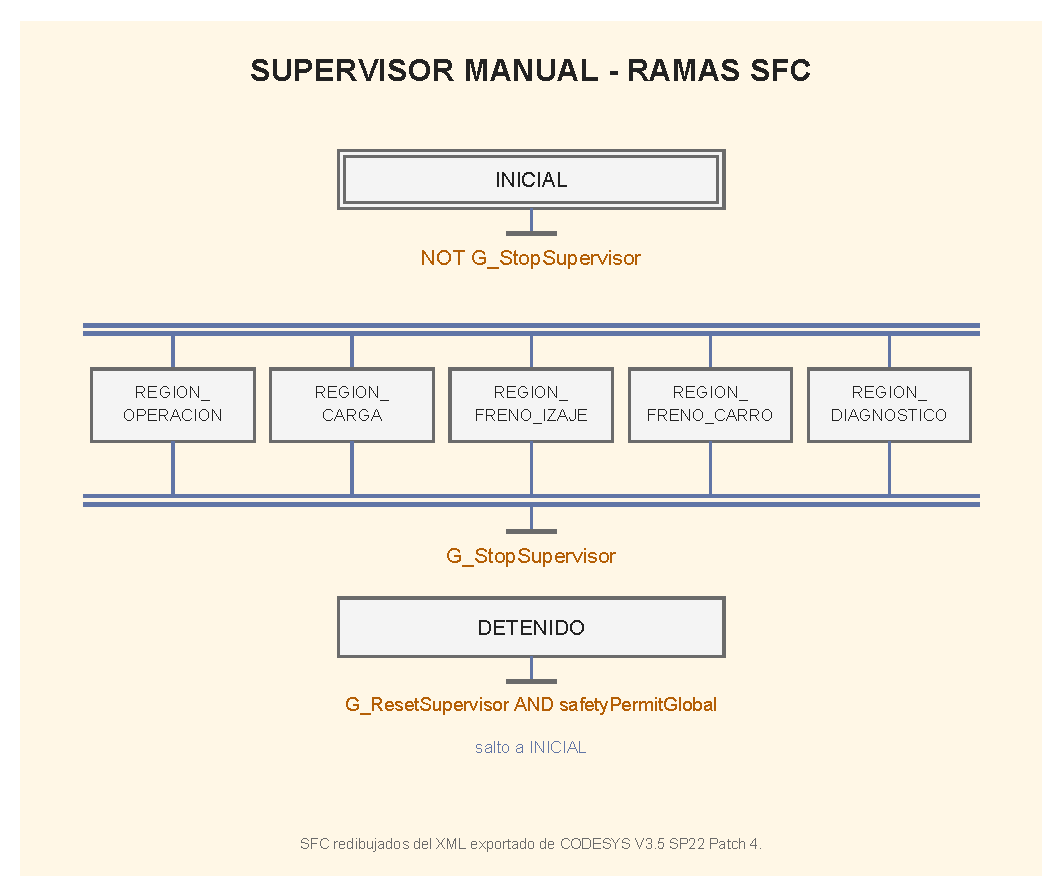
\includegraphics[width=0.96\textwidth]{diagramas_codesys_manual/12_sfc_supervisor_paralelo.pdf}
\caption{SFC contenedor del supervisor manual. La divergencia y convergencia son simultáneas; la ejecución de los restantes POUs depende de la lista de llamadas de la tarea.}
\label{fig:sfc_supervisor_manual}
\end{figure}


\subsection{Secuencias SFC de operación y transferencia de modo}
La región \texttt{OPERACION} de Stateflow se reparte entre tres SFC principales. \path{SFC_CICLO_SISTEMA} recorre \texttt{APAGADO}, \texttt{ARRANQUE}, \texttt{LISTO} y \texttt{PARADA\_NORMAL}. \texttt{LISTO} permanece activo durante las maniobras y funciona como habilitación de los SFC de modo; no equivale exclusivamente al código dos presentado por el HMI. El código efectivo se obtiene del arbitraje de salidas.

\path{SFC_MODO_MANUAL} contiene \texttt{MANUAL\_INACTIVO}, \texttt{MANUAL\_SUPERVISADO} y \path{APROXIMACION_FINAL_MANUAL}. La salida del manual supervisado hacia aproximación final ocurre por solicitud automática, solicitud de barrido o abandono del paso \texttt{LISTO}. Esta guarda difiere del Stateflow, donde la aproximación final se selecciona después del retorno desde un automático completado.

\path{SFC_MODO_AUTO} contiene espera, transferencia a automático, automático y transferencia a manual. Toda entrada recorre \path{BUMPLESS_A_AUTO}, con una permanencia mínima de $40~\mathrm{ms}$. Exige \texttt{LISTO} activo, solicitud e inicio automático, perfil válido, altura local suficiente, ausencia de sobrecarga y ausencia de intervención. No reproduce la entrada directa \texttt{LISTO} a \texttt{AUTOMATICO} del chart. El retorno a inactivo admite \texttt{allStopped}, que exige velocidades menores que $0.03~\mathrm{m/s}$ en ambos ejes, o la pérdida de \texttt{LISTO}.

\begin{figure}[!htbp]
\centering
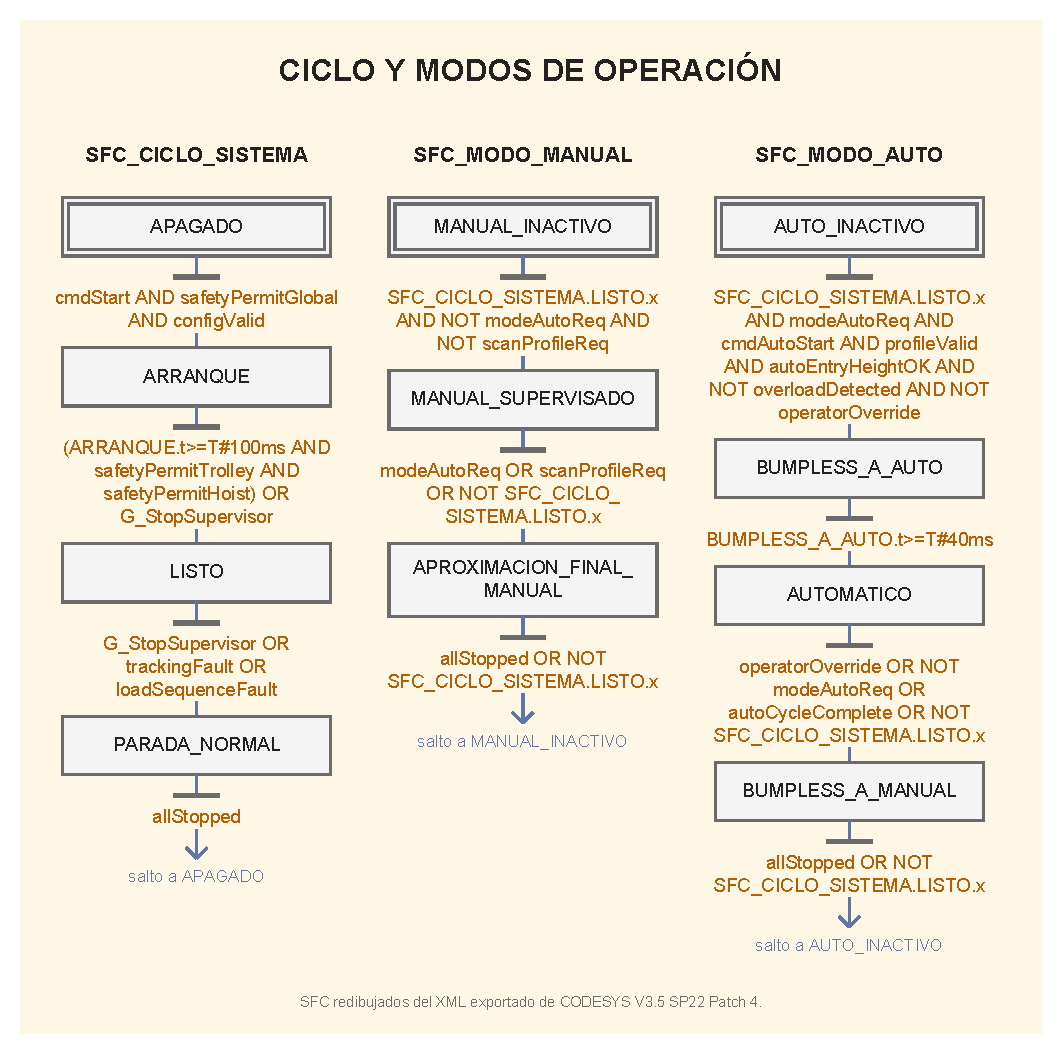
\includegraphics[width=0.98\textwidth,height=0.72\textheight,keepaspectratio]{diagramas_codesys_manual/13_sfc_operacion.pdf}
\caption{SFC de ciclo, manual y automático. Las condiciones son las expresiones exportadas del proyecto, incluidas las referencias a pasos activos de otros POUs.}
\label{fig:sfc_modos_manual}
\end{figure}


\subsection{SFC de barrido LiDAR y ejecución automática}
\path{SFC_ESCANEO_LIDAR} añade \texttt{ESPERA\_ESCANEO} a los cuatro pasos funcionales del relevamiento. Para comenzar exige \texttt{LISTO}, solicitud pendiente, perfil no completado, conjunto vacío y ejes detenidos. La preparación eleva hasta $39.65~\mathrm{m}$ con velocidad vertical pequeña. La condición derecha utiliza el límite normal o \texttt{lidarX}$\geq45.90~\mathrm{m}$ con velocidad pequeña; el Stateflow compara la posición del carro con $48.40~\mathrm{m}$. Se conserva el extremo izquierdo de $-24.50~\mathrm{m}$. La inicialización, registro y validación del perfil se efectúan en ST según el paso activo, incluida la precarga del \textit{slot} 33.

El XML del barrido es una cadena lineal: no contiene las transiciones laterales de parada o falla del chart. La pérdida de permisos se atiende mediante el ciclo principal y los interbloqueos de las salidas; no se dibujan rutas de escape inexistentes en este SFC.

\path{SFC_AUTOMATICO} recorre \texttt{ESPERA\_AUTO}, \texttt{PLANIFICAR}, \texttt{EJECUTAR} y \texttt{MANTENER\_OBJETIVO}. La planificación dura al menos $20~\mathrm{ms}$ y la llegada conserva los errores menores que $0.08~\mathrm{m}$ y $0.15~\mathrm{m}$. Las referencias se calculan en \path{PRG_ACCIONES_Y_SALIDAS}. Este proyecto utiliza el bloque \path{FB_craneTrajectoryQuintic}, con inicialización y evaluación explícitas, sin convertir los autómatas manuales en autómatas generados. La envolvente local, el objetivo seguro y la habilitación anti-sway siguen los criterios descritos para la referencia. La espera previa al descenso pertenece al planificador, no a una transición añadida al SFC.

\begin{figure}[!htbp]
\centering
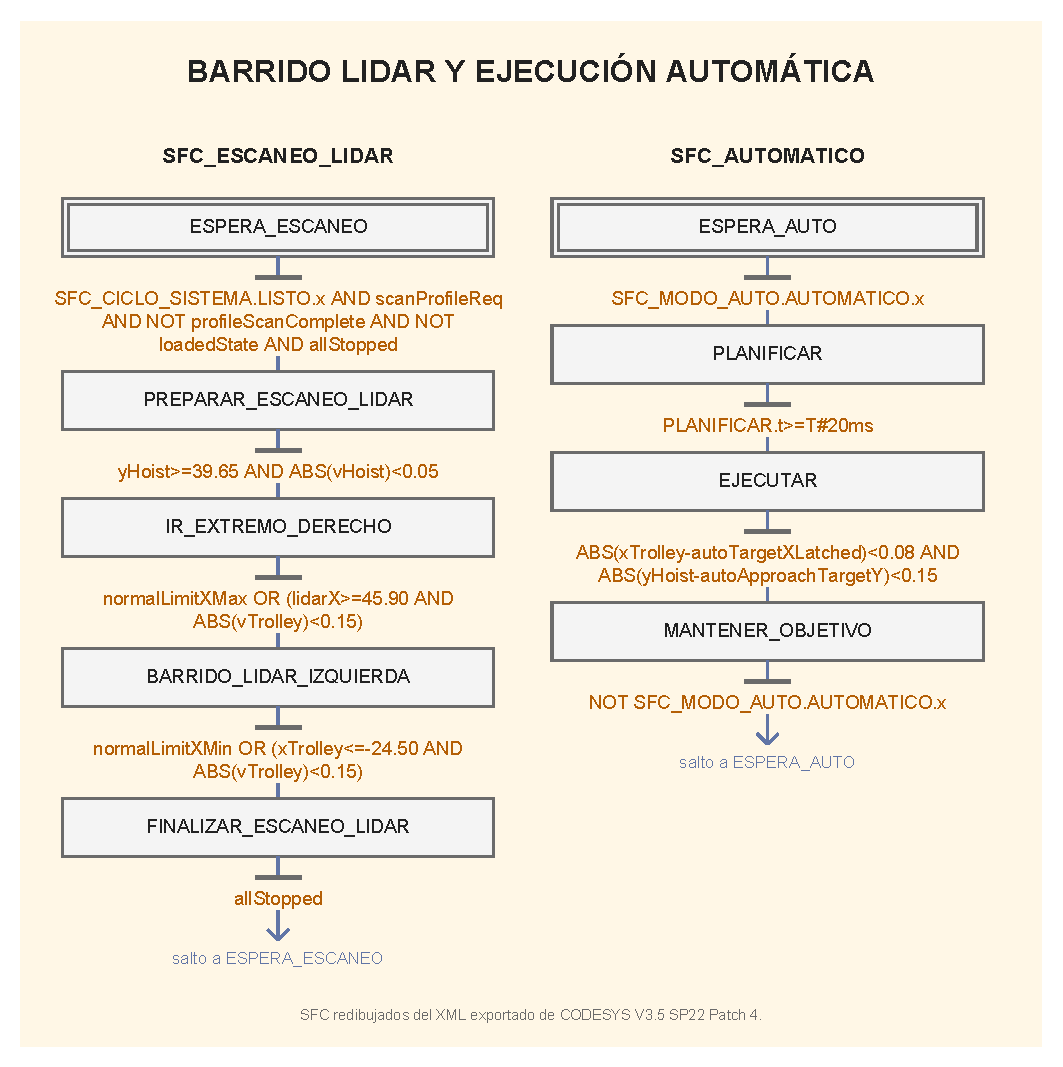
\includegraphics[width=0.98\textwidth,height=0.70\textheight,keepaspectratio]{diagramas_codesys_manual/14_sfc_barrido_automatico.pdf}
\caption{SFC de relevamiento y automático interno de la versión manual de CODESYS. Las cadenas retornan por saltos a sus pasos iniciales.}
\label{fig:sfc_barrido_auto_manual}
\end{figure}


\subsection{SFC de carga, pesaje y twistlocks}
La secuencia principal \path{SFC_CARGA} posee siete pasos: vacío, espera de estabilidad, cierre, despegue, pesaje, cargado y apertura. Conserva el contacto y permiso de izaje para iniciar el cierre, la estabilidad del spreader y las condiciones de cable tenso, velocidad y aceleración para iniciar el pesaje. En ST se acumula masa mientras \texttt{PESAJE.x} es verdadero; tras $500~\mathrm{ms}$ el SFC pasa a \texttt{CARGADO}.

Sobrecarga y falla de twistlocks se supervisan en POUs separados. \path{SFC_SOBRECARGA} detecta masa mayor que $50000~\mathrm{kg}$ con \texttt{CARGADO} activo. \path{SFC_FALLO_TWISTLOCK} detecta seguimiento fallido o permanencia de al menos $2~\mathrm{s}$ en cierre o apertura. Estas condiciones inhiben salidas mediante \texttt{loadSequenceFault}; no constituyen estados alternativos dentro de \path{SFC_CARGA}.

En Stateflow, el pesaje bifurca directamente hacia \texttt{CARGADO} o \texttt{SOBRECARGA}, y la espera de estabilidad puede cancelarse retornando a vacío. El SFC exportado no contiene esa cancelación ni la salida de despegue hacia apertura. Tampoco posee una transición de reinicio que reposicione por sí misma la cadena de carga al reconocer una falla. Estas diferencias explican por qué un reconocimiento del HMI no debe confundirse con un reinicio del estado interno de todos los SFC.

\begin{figure}[!htbp]
\centering
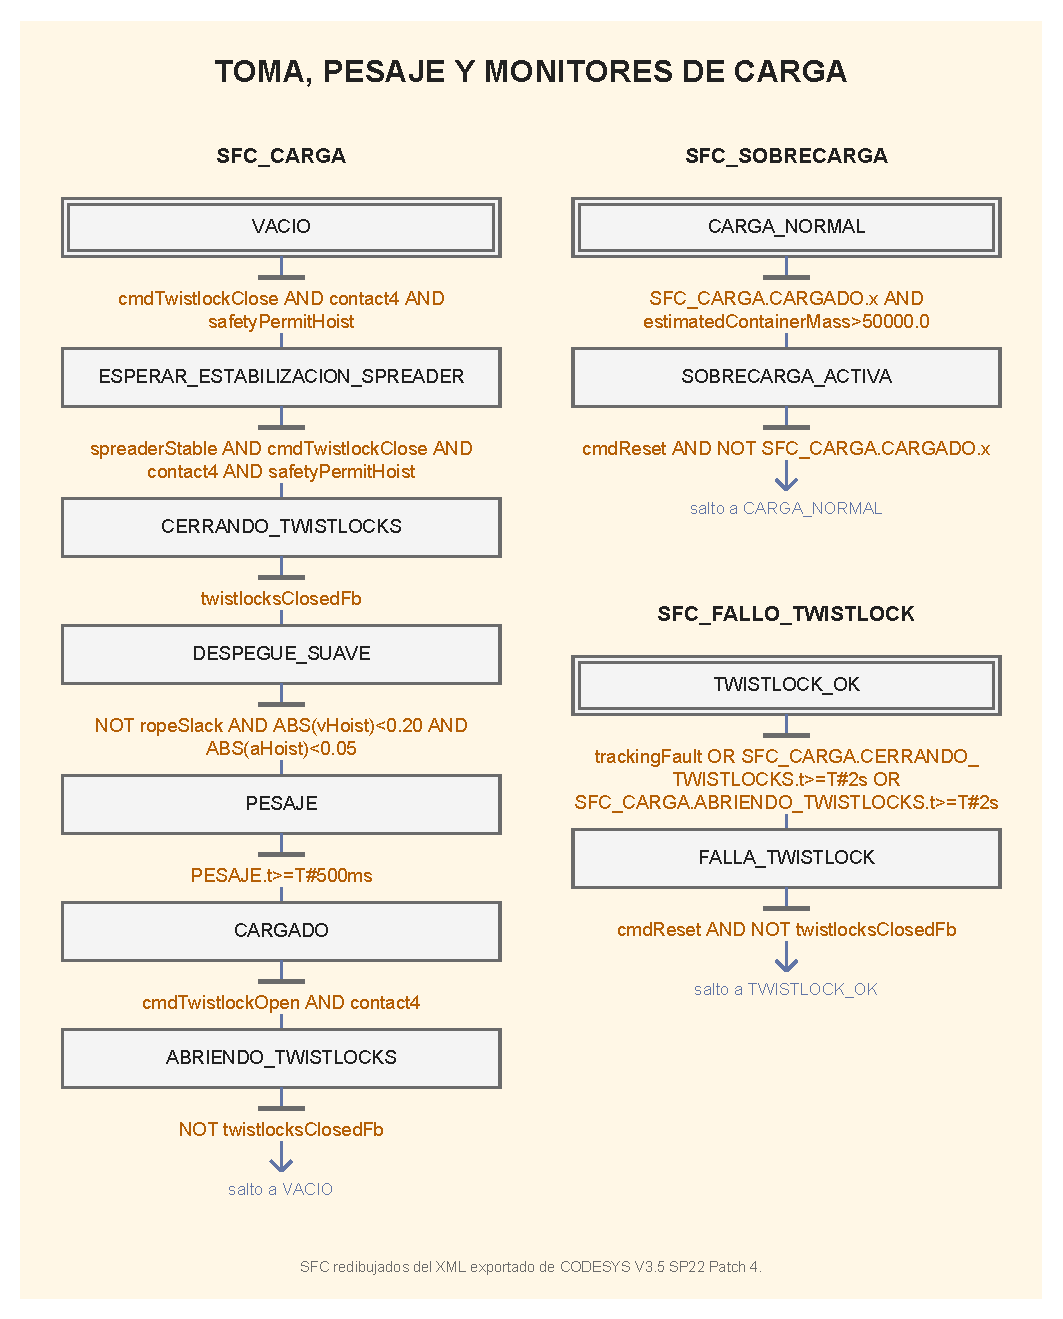
\includegraphics[width=0.98\textwidth,height=0.73\textheight,keepaspectratio]{diagramas_codesys_manual/15_sfc_carga.pdf}
\caption{Cadena SFC de carga y monitores separados de sobrecarga y twistlocks. No se agregan bifurcaciones que solamente existen en el chart de Stateflow.}
\label{fig:sfc_carga_manual}
\end{figure}


\subsection{SFC de frenos y comprobación de torque}
Los SFC de freno conservan los cuatro pasos aplicado, prueba de torque, abierto y aplicando. En izaje se conserva el criterio vertical de $0.05~\mathrm{m}$ y la excepción del modo automático ante ausencia momentánea de demanda. Sin embargo, el SFC de izaje no vuelve al paso aplicado por timeout de prueba; un monitor separado declara falla al superar $1~\mathrm{s}$ sin torque comprobado.

En carro se utiliza una tolerancia horizontal de $0.05~\mathrm{m}$, frente a $0.03~\mathrm{m}$ del chart. La transición desde prueba hacia abierto admite torque comprobado o cancelación de demanda, habilitación o permiso. El paso \texttt{TB\_ABIERTO} por sí solo no abre físicamente el freno: ST exige \texttt{brakeTrolleyProofLatched}, regulador habilitado, permisos y ausencia de falla de carga. La prueba queda memorizada para la maniobra vigente y se borra ante cancelación, pérdida de permiso o retorno a aplicado.

El monitor de carro declara falla tras $8~\mathrm{s}$ de prueba sin torque, únicamente si persisten habilitación, permiso y demanda. Es una adaptación de la versión ensayada con el simulador, distinta del retorno por $50$ ticks del Stateflow. Los monitores de ambos frenos se incorporan a \texttt{loadSequenceFault}. Esta separación entre avance del SFC y salida física debe conservarse al interpretar los diagramas.

\begin{figure}[!htbp]
\centering
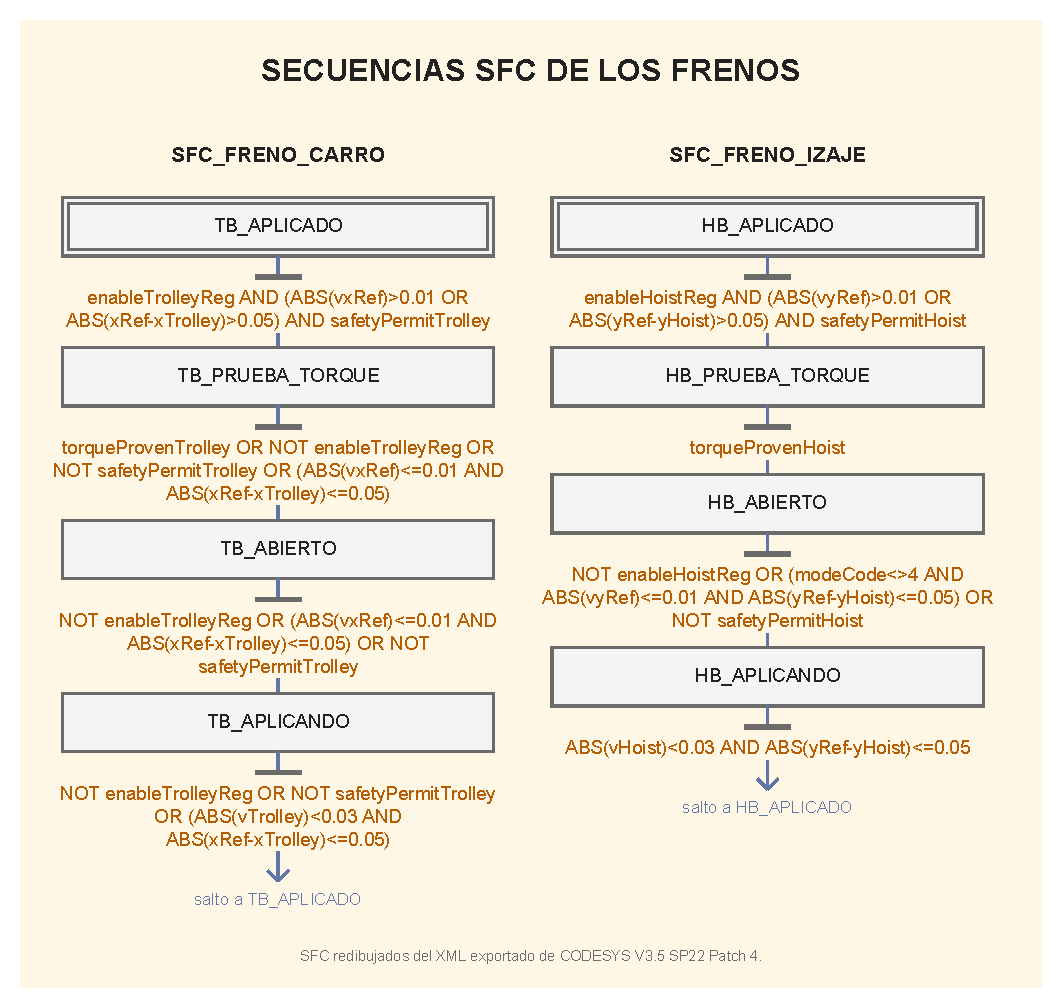
\includegraphics[width=0.98\textwidth,height=0.68\textheight,keepaspectratio]{diagramas_codesys_manual/16_sfc_frenos.pdf}
\caption{Secuencias SFC de los frenos. Las autorizaciones físicas finales se calculan en ST y pueden ser más restrictivas que el paso activo.}
\label{fig:sfc_frenos_manual}
\end{figure}


\begin{figure}[!htbp]
\centering
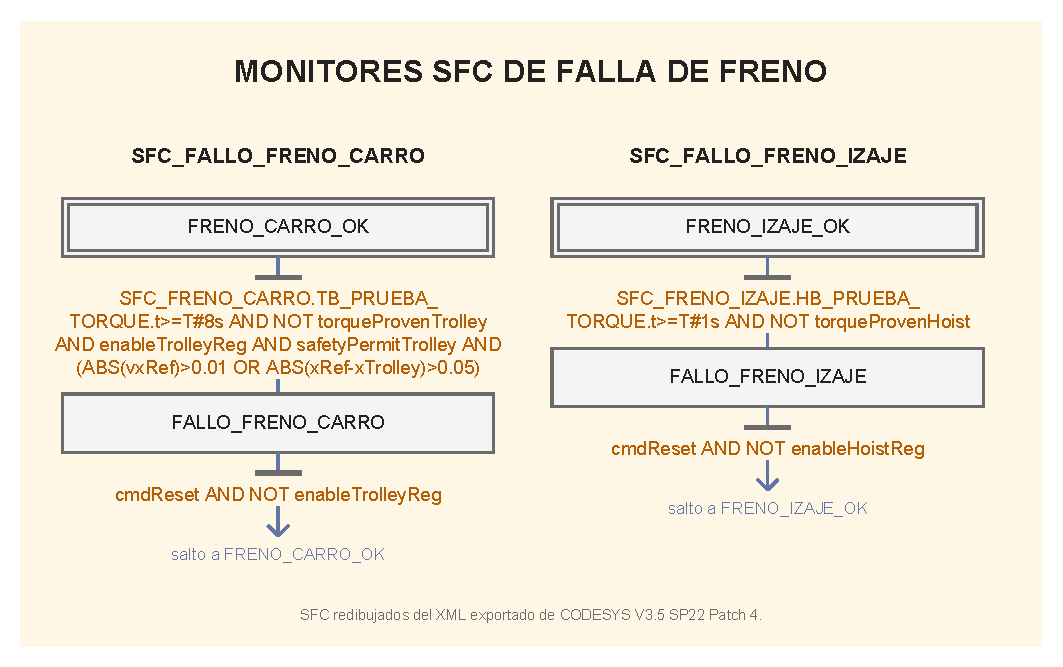
\includegraphics[width=0.98\textwidth]{diagramas_codesys_manual/16b_sfc_fallas_frenos.pdf}
\caption{Monitores de falla de los frenos del carro y del izaje, con timeout y reconocimiento independientes.}
\label{fig:sfc_fallas_frenos_manual}
\end{figure}

\subsection{SFC de cuerda floja y diagnóstico}
\path{SFC_CUERDA_FLOJA} materializa la histéresis de tensión mediante dos pasos: cambia a cuerda tensa por encima de $15000~\mathrm{N}$ y retorna a floja por debajo de $12000~\mathrm{N}$. En Stateflow esta memoria se implementa en una función auxiliar.

\path{SFC_ALARMA_SOBRECARGA} y \path{SFC_FALLO_SUPERVISOR} son monitores de dos pasos. El primero reconoce la alarma con reinicio y desaparición de sobrecarga; el segundo retiene seguimiento fallido, falla de carga o ausencia de permiso global. Los códigos se calculan en preprocesamiento y se publican en el arbitraje final. Como varios pasos pueden estar activos simultáneamente, la prioridad efectiva depende de las ramas \texttt{IF/ELSIF} del programa ST, además del orden de llamadas. No corresponde atribuirles el único estado exclusivo \texttt{DIAG\_OK/ALARMA/FALLA} del chart.

\begin{figure}[!htbp]
\centering
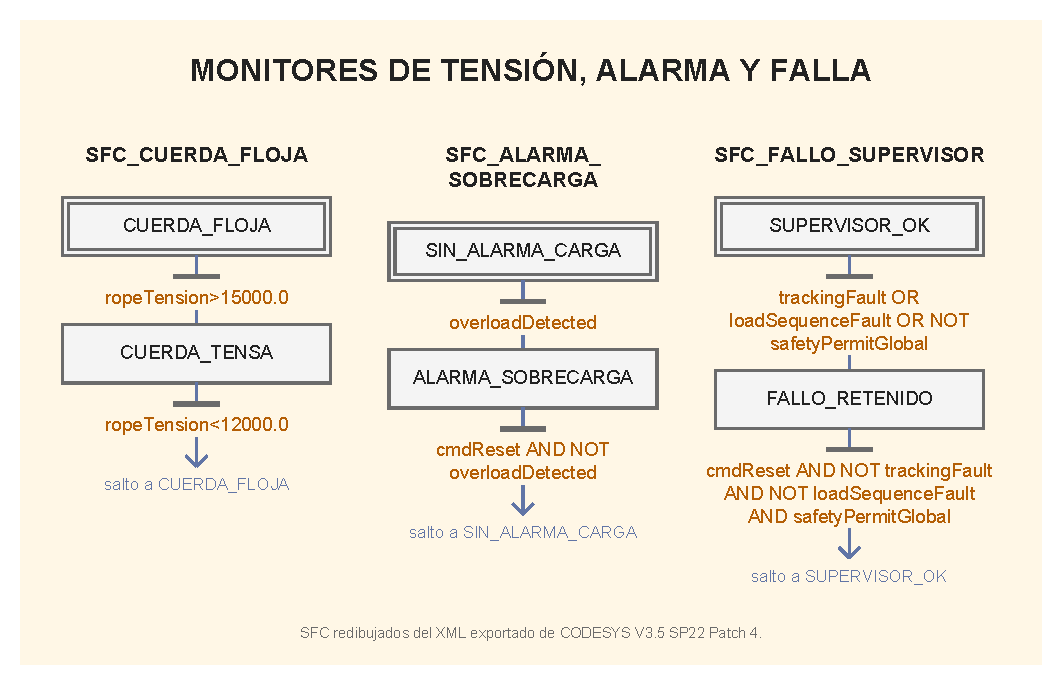
\includegraphics[width=0.98\textwidth]{diagramas_codesys_manual/17_sfc_diagnostico.pdf}
\caption{SFC auxiliares de tensión, alarma por sobrecarga y falla retenida del supervisor manual.}
\label{fig:sfc_diag_manual}
\end{figure}


\subsection{Comparación del supervisor: Stateflow y CODESYS manual}
Ambas implementaciones comparten las señales físicas, los objetivos locales, la toma estable, la generación de referencias y los permisos de seguridad. La traducción manual distribuye la secuencia y sus acciones entre POUs; conserva el objetivo funcional, pero no constituye una equivalencia completa del grafo jerárquico ni de sus prioridades.

{\footnotesize
\begin{longtable}{L{3.0cm} L{5.8cm} L{5.8cm}}
\caption{Correspondencias y diferencias verificadas del supervisor.}\label{tab:comparacion_sup_sfc}\\
\toprule
Aspecto & Stateflow de referencia & CODESYS manual SFC\\
\midrule
\endfirsthead
\toprule Aspecto & Stateflow de referencia & CODESYS manual SFC\\\midrule
\endhead
Organización & Cinco regiones paralelas dentro de un chart; frenos con dos subregiones. & Dieciséis programas SFC y programas ST de preprocesamiento/salidas llamados por una tarea.\\
Acciones & Entrada, ejecución y salida de estados; funciones MATLAB del chart. & Estados consultados mediante \texttt{Paso.x}; acciones en ST, sin bloques de acción en los SFC exportados.\\
Estado listo & Estado de operación previo a seleccionar manual o automático. & Paso del ciclo que permanece activo y habilita secuencias de modo independientes.\\
Entrada automática & Directa desde LISTO; desde manual utiliza dos ticks de transferencia. & Siempre utiliza BUMPLESS\_A\_AUTO con al menos 40 ms; añade ausencia de intervención desde LISTO.\\
Guarda automática & Desde manual exige ciclo no completo; altura local y perfil válido en ambas entradas. & Conserva perfil y altura local; la guarda de entrada no comprueba \texttt{autoCycleComplete}.\\
Salida automática & Bumpless hacia manual por objetivo, intervención o cancelación. & Añade pérdida de LISTO; retorno por \texttt{allStopped} o pérdida de LISTO.\\
Aproximación manual & Posterior al automático completado; sale al liberar carga. & Paso del SFC manual alcanzado por solicitud auto/barrido o pérdida de LISTO; sale por reposo o pérdida de LISTO.\\
Barrido & Estados con salidas laterales de parada/falla; extremo derecho en \texttt{xTrolley}. & Cadena sin escapes laterales; extremo derecho en \texttt{lidarX}; inhibición final de salidas en ST.\\
Carga y sobrecarga & Bifurcación de pesaje a cargado/sobrecarga; falla y cancelación dentro de la región. & Pesaje de 500 ms a cargado; sobrecarga y falla en monitores separados.\\
Freno del carro & Prueba de torque con retorno por 50 ticks; tolerancia de posición 0.03 m. & Monitor de 8 s; tolerancia de 0.05 m; prueba memorizada necesaria para apertura física.\\
Freno de izaje & Retorno al aplicado por timeout de 50 ticks. & Monitor separado de 1 s sin transición de timeout en la secuencia del freno.\\
Diagnóstico & Máquina exclusiva OK/alarma/falla. & Monitores concurrentes y arbitraje de códigos en ST.\\
Tiempo & Ticks y segundos del motor de simulación de Stateflow. & Permanencia \texttt{Paso.t} y acumuladores en la tarea PLC de 20 ms; tiempo de pared.\\
\bottomrule
\end{longtable}}

Los diagramas SFC permiten inspeccionar la secuencia real y la tabla permite localizar los cambios de estructura. La comparación no demuestra equivalencia temporal de todos los eventos concurrentes; en las pruebas OPC UA, Simulink y el PLC no están sincronizados por pasos. El planificador quíntico generado dentro del proyecto manual no cambia el lenguaje SFC de estos autómatas.



\subsection{Implementación automática del supervisor en CODESYS}
La implementación automática del supervisor y del autómata de seguridad se realizó mediante la generación automática de código para PLC de Simulink, utilizando Simulink PLC Coder con destino CODESYS.

La generación produce XML de intercambio con cuerpos en Structured Text. No produce diagramas SFC nuevos: la representación gráfica de referencia sigue siendo el chart de Stateflow de las Figuras anteriores. El bloque principal \path{FB_GEN_SUPERVISOR} representa la jerarquía mediante variables de estado, constantes, estructuras \texttt{CASE}, condiciones y funciones auxiliares. Los comentarios del ST conservan referencias a elementos del modelo. Las acciones de entrada, ejecución y salida quedan integradas en ese código, en lugar de repartirse entre pasos SFC y programas de acciones escritos manualmente.

La salida original contiene 27 POUs del supervisor y 3 de protección. Estos recuentos incluyen bloques auxiliares y no son números de estados. La integración utiliza tres llamadas en \path{MainTask_20ms}, en este orden: \path{PRG_ENLACE_OPCUA}, \path{PRG_AUTO_SEGURIDAD} y \path{PRG_AUTO_SUPERVISOR}. La tarea tiene intervalo de 20 ms, prioridad 1 y watchdog de 100 ms. En la copia automática final se retiraron los 21 SFC manuales. Tener el ST generado importado junto a los SFC antiguos no basta para identificar qué implementación está activa: debe verificarse también la lista de llamadas de la tarea.

Los adaptadores inicializan cada instancia una vez con \texttt{SS\_INITIALIZE} y luego ejecutan \texttt{SS\_STEP} en cada llamada. La planta, los reguladores, los sensores, el HMI y la visualización permanecen en Simulink. OPC UA intercambia medidas y órdenes mediante \path{GVL_GRUA}; el adaptador no traslada al PLC la dinámica de la grúa.

\subsection{Adaptaciones de importación e interfaz}
El adaptador conecta 33 entradas y 39 salidas del supervisor. Cuatro entradas cambian de nombre al conectarse con la interfaz existente: \texttt{omega\_td\_est} recibe \texttt{omegaTrolley}, \texttt{y\_l} recibe \texttt{yHoist}, \texttt{v\_ly} recibe \texttt{vHoist} y \texttt{F\_hw\_sens} recibe \texttt{ropeTension}. Convierte \texttt{modeCode} de \texttt{LREAL} a \texttt{INT} y copia los perfiles de índices $[0..32]$ del bloque generado a los índices $[1..33]$ de OPC UA. Un desplazamiento incorrecto de índices cambiaría la correspondencia física de los slots.

Después del STEP se aplican compuertas de permisos a habilitaciones y órdenes de apertura de frenos. Si se ordena cerrar twistlocks se fuerza a falso su orden de apertura. Estas operaciones pertenecen a la integración escrita para CODESYS; no deben atribuirse a una transformación automática del chart. Asimismo, el temporizador generado para protección requiere el tipo calificado \texttt{Standard.TON} en esta instalación y la biblioteca Standard utilizada por el proyecto.


\subsection{Diferencia temporal detectada en la generación}
El principal problema encontrado al ejecutar la primera versión no fue una guarda de transición distinta, sino una incompatibilidad entre la base temporal del código exportado y la tarea que lo llamaba. La cabecera del XML original declara una muestra de subsistema de $1~\mathrm{ms}$. PLC Coder insertó contadores con divisores 20 y 40 para atender tasas de 20 y 40 ms del modelo. Esos divisores sólo mantienen las tasas esperadas si la llamada externa conserva la base de 1 ms.

La tarea CODESYS llamaba al bloque cada 20 ms. Por ello, el primer divisor activaba la lógica del supervisor cada $20\times20=400~\mathrm{ms}$; la segunda tasa pasaba a $40\times20=800~\mathrm{ms}$. Los pulsos del HMI de 40 ms podían quedar completos entre dos ejecuciones de la lógica. En el intento registrado, la comunicación cifrada funcionó, pero el modo permaneció en cero durante 186.72 s de simulación después de START y no comenzó el barrido. Una nueva pulsación tampoco inició la secuencia.

La corrección se aplicó al ST preparado para importación: los umbrales de los contadores se cambiaron de 19 y 39 a 0 y 1, respectivamente. Así, con la tarea de 20 ms, el primer grupo se atiende en cada llamada y el segundo cada dos llamadas.

\begin{table}[!htbp]
\centering\small
\caption{Tasas del código generado y adaptación a la tarea PLC.}\label{tab:tasas_plc_coder}
\begin{tabular}{L{4.3cm} C{3.1cm} C{3.1cm} C{3.1cm}}
\toprule
Grupo & Divisor original & Con tarea de 20 ms & Divisor corregido\\
\midrule
Tasa de 20 ms & 20 llamadas & 400 ms & 1 llamada: 20 ms\\
Tasa de 40 ms & 40 llamadas & 800 ms & 2 llamadas: 40 ms\\
\bottomrule
\end{tabular}
\end{table}

Los temporizadores IEC de protección usan el reloj del runtime, mientras los contadores de muestras dependen del número de activaciones. Además, el ensayo usa Accelerator sin pacing: el tiempo simulado de la planta y el reloj del PLC no avanzan de forma determinista conjunta. Corregir los divisores resuelve la tasa de llamada del supervisor; no convierte la comunicación OPC UA en una cosimulación sincronizada paso a paso. Los tiempos de los resultados que siguen son tiempos de simulación.

\subsection{Inicialización del perfil para la prueba de medio ciclo}
La prueba de medio ciclo comienza con un perfil físico conocido de 33 alturas y no incluye barrido LiDAR. En la implementación automática, el perfil y su validez pertenecen a la memoria interna de \texttt{fbSupervisor}. El adaptador copia sus salidas hacia \path{GVL_GRUA} cada ciclo. Escribir desde OPC UA solamente el perfil o \texttt{profileValid} en esa GVL no inicializa la memoria del autómata: se observó que la validez escrita volvía a falso después de 120 ms y que el máximo permanecía en $-20~\mathrm{m}$.

Para inicializar el perfil interno, el supervisor añade la entrada \texttt{testInitialProfile} y el método \texttt{ssMethodType=2}, que copia las 33 alturas dentro de la instancia únicamente en modo apagado, sin carga y sin perfil válido. Declara válido el perfil, pero conserva \texttt{profileScanComplete=false}: no representa un relevamiento realizado. El STEP habitual calcula máximo y envolvente. Los casos originales INITIALIZE y STEP y las funciones de secuencia se conservan; esta extensión es código agregado para el banco de ensayo y no una salida íntegramente automática de PLC Coder. La protección no se modifica.

Un primer intento de precarga también mostró una carrera entre la escritura del vector y la solicitud de validez, enviadas en servicios OPC UA separados. El adaptador podía reemplazar el vector entre ambos. El iniciador se corrigió para enviar el vector completo y después la habilitación dentro del mismo servicio Write, y comprobar el resultado por lectura. Esta solución reúne la solicitud en una operación del cliente; no se asume atomicidad general del servidor. El intento incoherente se detuvo antes de START y no se cuenta como maniobra. Antes de repetir se hizo Reset en caliente y RUN para limpiar la memoria de la instancia. El RESET del HMI no equivale a esta reinicialización.


\subsection{Comparación con Stateflow y con la traducción manual}
La versión automática mantiene como fuente los charts jerárquicos descritos en este capítulo. Por ello conserva en el núcleo generado las ramas, prioridades y acciones de esa referencia, incluidas las salidas de cancelación de carga y los estados de falla que no aparecen como bifurcaciones dentro de la cadena SFC manual. La comparación de la fuente y la lectura del ST sustentan esa correspondencia; la integración introduce modificaciones propias que deben comprobarse por separado.

{\footnotesize
\begin{longtable}{L{3.0cm} L{5.8cm} L{5.8cm}}
\caption{Diferencias entre implementación manual y automática.}\label{tab:manual_auto_st}\\
\toprule Aspecto & CODESYS manual & CODESYS automático\\\midrule
\endfirsthead
\toprule Aspecto & CODESYS manual & CODESYS automático\\\midrule
\endhead
Fuente de secuencia & Traducción a 21 SFC con acciones y cálculos en ST auxiliar. & Dos charts Stateflow, convertidos a bloques y auxiliares ST.\\
Representación & Pasos y transiciones visibles en CODESYS. & Variables de estado, constantes y CASE; los gráficos se consultan en Stateflow.\\
Tarea & 26 llamadas explícitas a enlace, monitores, secuencias y salidas. & Tres llamadas: enlace, adaptador de seguridad y adaptador de supervisor.\\
Acciones & Programas separados leen pasos activos y tiempos de permanencia. & Acciones y prioridades traducidas dentro del bloque generado.\\
Base temporal & Secuencias llamadas por tarea de 20 ms. & Divisores exportados desde base de 1 ms; requirieron adaptación a 20 ms.\\
Perfil retenido & Perfil gestionado por variables y programas de la aplicación manual. & Perfil interno en la instancia del bloque; precarga mediante método específico del ensayo.\\
Emergencias & Monitores independientes por eje y watchdog antes de total. & Núcleo conserva estados exclusivos y orden de regiones del chart; permisos finales calculados por adaptador.\\
Mantenimiento & Cambios realizados en SFC y soporte ST. & Cambios de secuencia en Stateflow, regeneración y preparación de importación; adaptación de ensayo mantenida por separado.\\
Resultados de maniobra & Sin antisway incompleta; con antisway completada. & Mismo resultado cualitativo en el ensayo de medio ciclo.\\
\bottomrule
\end{longtable}}

La generación informó nombres de datos locales que sombrean nombres de niveles superiores y una entrada \texttt{finalApproachDistance} no utilizada. Son observaciones del modelo fuente, diferentes de las advertencias del compilador CODESYS. Los registros de compilación de la copia de 20 ms y de la copia de medio ciclo indican cero errores y cero advertencias. Esto comprueba integración sintáctica y de tipos, pero por sí solo no valida una maniobra ni demuestra equivalencia completa.

\subsection{Resultados disponibles y alcance de la validación}
Las pruebas actualizadas comparan CODESYS manual y CODESYS automático, cada uno con y sin antisway, sobre una misma planta y procedimiento de medio ciclo. La toma y el despegue son manuales; el traslado es automático; el apoyo y la descarga vuelven a ser manuales. El perfil se precarga desde la escena y no se realiza relevamiento ni retorno vacío.

La prueba CODESYS manual con antisway confirmó entrega y parada a $169.20~\mathrm{s}$. CODESYS manual sin antisway se detuvo a $187.20~\mathrm{s}$ y CODESYS automático sin antisway a $180.00~\mathrm{s}$, ambos con carga retenida. CODESYS automático con antisway se detuvo por diagnóstico a $279.52~\mathrm{s}$: el PLC indicó descarga, pero la planta mantuvo el contenedor suspendido. Esta discrepancia impide declarar completada la entrega.

La descripción detallada, las señales y las limitaciones de registro se presentan en las \cref{sec:ensayo_codesys_manual,sec:ensayo_codesys_st,sec:comparacion_ensayos_codesys}. Los ensayos evalúan la integración de los autómatas con la planta simulada; no certifican el relevamiento, equivalencia completa de estados ni seguridad de una grúa física.

\clearpage
\section{Autómata de seguridad}
\subsection{Correspondencia con el modelo vigente}
La revisión del chart de protección confirma la misma estructura de dos regiones paralelas, cuatro estados de emergencia y dos estados de watchdog. Se mantienen las guardas por flanco, las polaridades de autorización de freno y el orden de ejecución. Por ello, los diagramas de emergencias y watchdog conservan su topología. Se explicitan aquí las prioridades y los tiempos para que esta sección corresponda con la misma referencia que el supervisor.

\subsection{Criterio de independencia}
El nivel de seguridad se encuentra en un subsistema separado y no depende del estado interno del supervisor para detectar una condición peligrosa. Recibe directamente el pulsador de emergencia, los límites últimos, el exceso de velocidad vertical, el pulso de \textit{watchdog} y la orden de reinicio.

El chart \texttt{Automata de proteccion} entrega las señales \texttt{BRK\_t}, \texttt{BRK\_h}, \texttt{BRK\_hE}, \texttt{EMERGENCIA} y \path{PARADA_EMERGENCIA_WD}. Fuera del chart, el subsistema convierte las tres primeras señales en permisos y órdenes de apertura de freno de acuerdo con
\begin{align}
\texttt{permitTrolley}&=\texttt{BRK\_t},\\
\texttt{permitHoist}&=\texttt{BRK\_h},\\
\texttt{permitGlobal}&=\texttt{BRK\_t}\ \mathrm{OR}\ \texttt{BRK\_h}.
\end{align}
Por ello, una emergencia limitada a un eje mantiene verdadero el permiso global y sólo la emergencia total lo lleva a cero. Las órdenes normales del supervisor se combinan posteriormente con estas autorizaciones, de modo que no pueden abrir un freno prohibido por el nivel de seguridad.

\begin{table}[!htbp]
\centering
\caption{Polaridad y significado de las salidas principales de seguridad.}\label{tab:polaridad_seguridad}
\begin{tabular}{L{3.4cm} C{2.0cm} C{2.0cm} L{6.2cm}}
\toprule
Señal & Normal & Intervención & Interpretación\\
\midrule
\texttt{BRK\_t} & 1 & 0 & Autorización para liberar el freno del carro.\\
\texttt{BRK\_h} & 1 & 0 & Autorización para liberar el freno operativo de izaje.\\
\texttt{BRK\_hE} & 1 & 0 & Autorización para liberar el freno de emergencia de izaje.\\
\texttt{EMERGENCIA} & 0 & 1 & Indicación general de una emergencia activa.\\
\path{PARADA_EMERGENCIA_WD} & 0 & 1 & Solicitud de emergencia total originada por el watchdog.\\
\bottomrule
\end{tabular}
\end{table}

En este informe las variables \texttt{BRK\_t}, \texttt{BRK\_h} y \texttt{BRK\_hE} se interpretan como autorizaciones activas en uno. Por ello, el valor cero implica intervención y no debe confundirse el nombre de la señal con el estado mecánico directo del freno. La operación OR utilizada para \texttt{permitGlobal} permite que una emergencia parcial conserve habilitado al eje no afectado; solamente cuando ambas autorizaciones de eje son falsas el permiso global se anula.

\begin{figure}[!htbp]
\centering
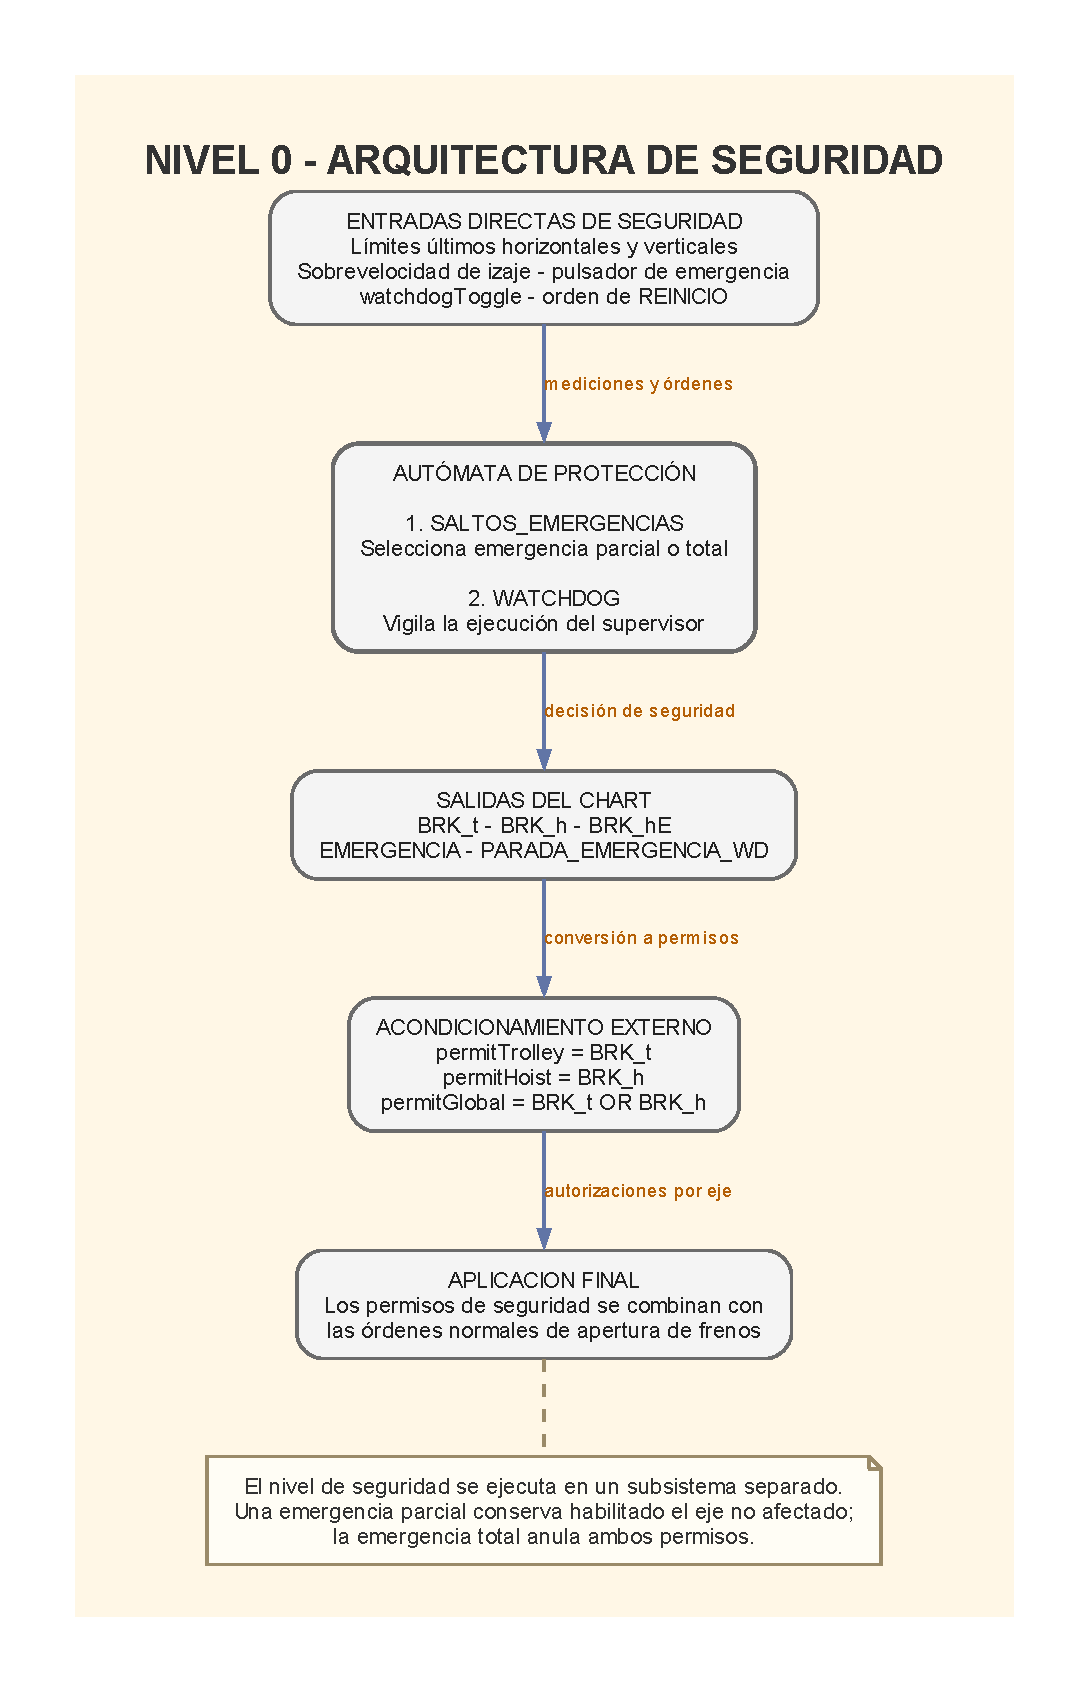
\includegraphics[height=0.60\textheight,keepaspectratio]{diagramas_automatas_revision/10_arquitectura_seguridad.pdf}
\caption{Ubicación funcional independiente del nivel de seguridad y flujo de sus señales.}
\label{fig:arquitectura_seguridad_vectorial}
\end{figure}


\subsection{Regiones del autómata de protección}
El Stateflow de seguridad contiene dos regiones paralelas. \texttt{SALTOS\_EMERGENCIAS} selecciona el tipo de emergencia y los frenos afectados. \texttt{WATCHDOG} verifica que el supervisor continúe ejecutándose.

Desde normal, las transiciones de emergencia se evalúan en este orden: emergencia total por pulsador o watchdog (prioridad 1), emergencia de izaje por flancos verticales o sobrevelocidad (prioridad 2) y emergencia del carro por flancos horizontales (prioridad 3). En cada emergencia parcial, el escalamiento a total precede a la recuperación. No se debe interpretar este orden como una evaluación simultánea independiente de todos los límites: si ambos ejes generan flancos en la misma activación desde normal, se toma primero la transición de izaje. El escalamiento posterior requiere el flanco indicado del otro eje o pulsador/watchdog; la matriz siguiente describe las causas reconocidas por esas guardas.

Los estados funcionales se indexan como:
\begin{table}[!htbp]
\centering
\caption{Estados del autómata de seguridad.}
\begin{tabular}{C{1.2cm} L{4.5cm} L{7.7cm}}
\toprule
Índice & Estado & Función\\
\midrule
S0 & \texttt{FUNCIONAMIENTO\_NORMAL} & Mantiene verdaderas las tres autorizaciones de apertura.\\
S1 & \texttt{EMERGENCIA\_CARRO} & Inhibe el carro y aplica su freno.\\
S2 & \texttt{EMERGENCIA\_IZAJE} & Inhibe izaje y aplica ambos frenos de izaje.\\
S3 & \texttt{EMERGENCIA\_TOTAL} & Inhibe todos los movimientos y aplica todos los frenos.\\
W0 & \texttt{FUNCIONAMIENTO\_NORMAL} & Reinicia temporización con cada cambio del pulso.\\
W1 & \texttt{FALLO\_WD} & Solicita parada total por pérdida de actividad.\\
\bottomrule
\end{tabular}
\end{table}

\begin{figure}[!htbp]
    \centering
    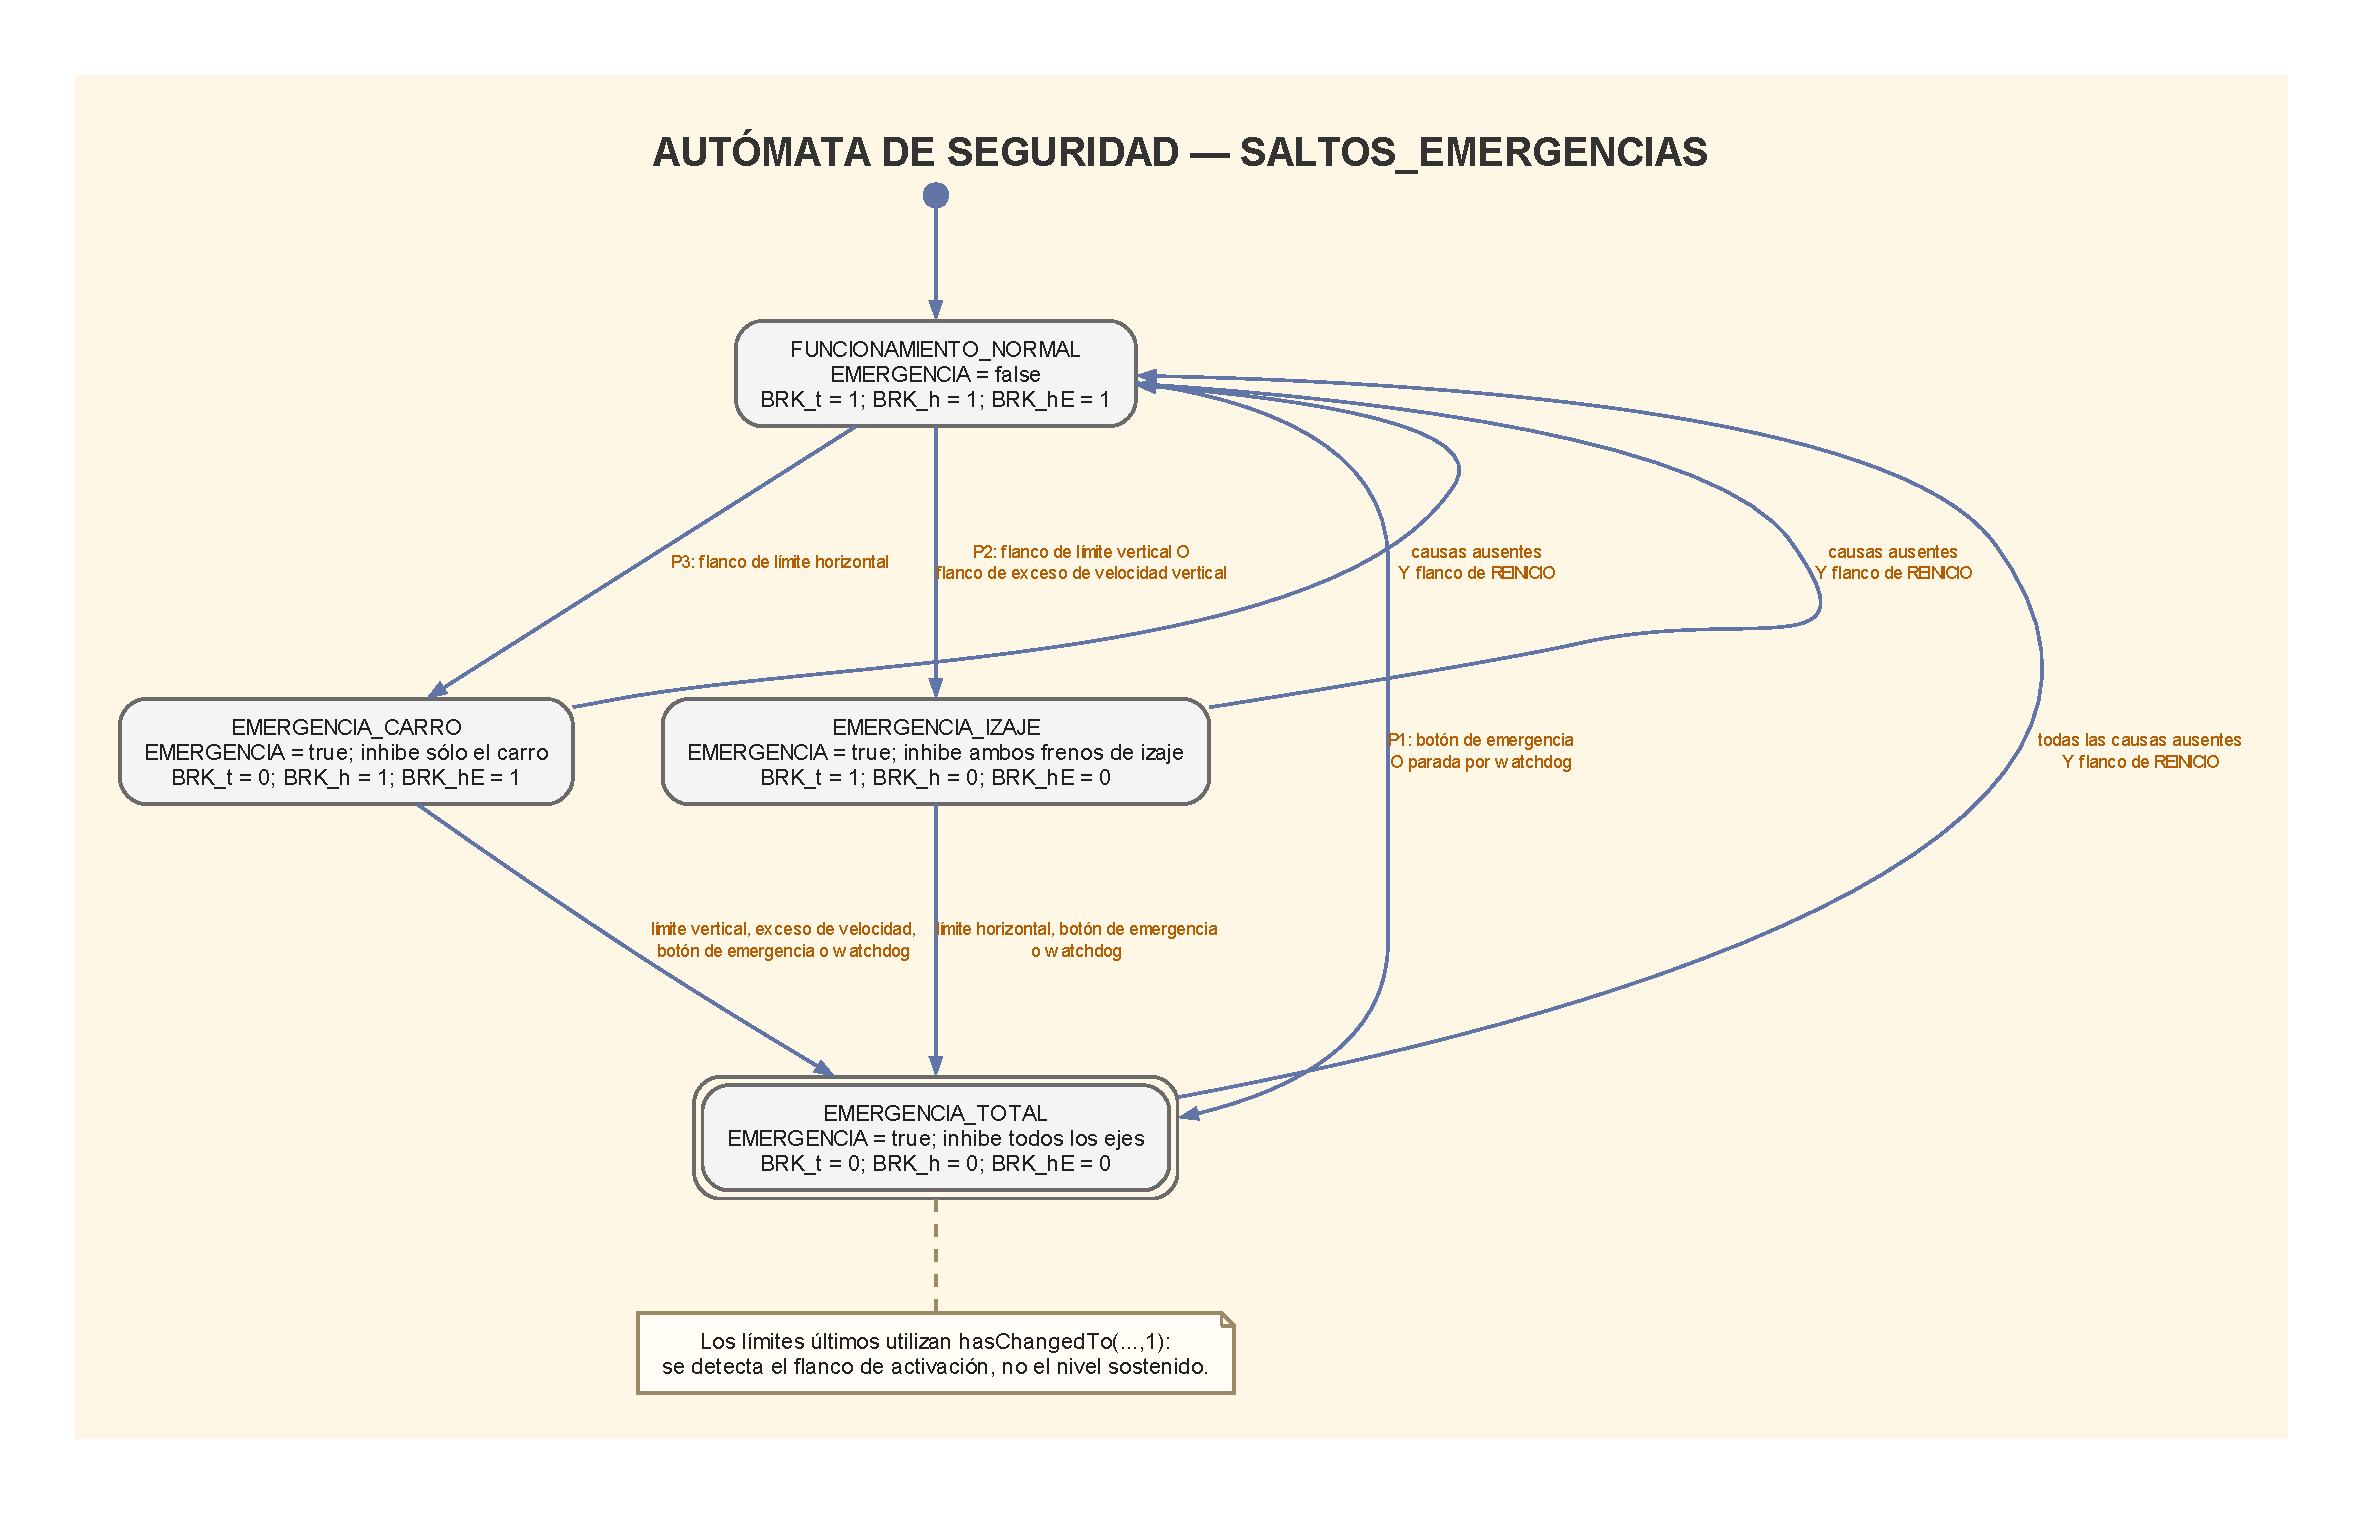
\includegraphics[width=0.98\textwidth,height=0.70\textheight,keepaspectratio]{diagramas_automatas_revision/08_seguridad_emergencias.pdf}
    \caption{Máquina de estados de la región \texttt{SALTOS\_EMERGENCIAS}, con prioridades, autorizaciones de freno y recuperación enclavada.}
\end{figure}


\subsection{Emergencia del carro}
Desde funcionamiento normal se ingresa a \texttt{EMERGENCIA\_CARRO} mediante \texttt{hasChangedTo(...,1)} sobre cualquiera de los límites últimos horizontales. La condición es sensible al flanco de activación y no sólo al nivel sostenido. En este estado \texttt{EMERGENCIA} pasa a verdadero, \texttt{BRK\_t} pasa a falso y \texttt{BRK\_h} y \texttt{BRK\_hE} permanecen verdaderos. Por lo tanto se aplica el freno del carro y el izaje continúa autorizado.

La recuperación exige que el pulsador de emergencia esté liberado, que ambos límites últimos horizontales estén inactivos y que se detecte un flanco de reinicio. No se permite una recuperación automática por la sola desaparición del límite.

Si durante una emergencia de carro aparece un límite último vertical, exceso de velocidad vertical, pulsador de emergencia o falla de \textit{watchdog}, se escala a \texttt{EMERGENCIA\_TOTAL}.


\subsection{Emergencia de izaje}
La emergencia de izaje se activa por un flanco ascendente del límite último superior, del límite último inferior o de la indicación de exceso de velocidad vertical. En este estado \texttt{BRK\_h} y \texttt{BRK\_hE} pasan a falso, mientras \texttt{BRK\_t} permanece verdadero. Se aplican ambos frenos de izaje y el carro continúa autorizado mientras no aparezca otra condición de emergencia.

Para recuperar se requiere que el pulsador esté liberado, que los límites verticales y la indicación de velocidad máxima estén inactivos y que exista un flanco de reinicio. Si aparece simultáneamente un límite horizontal, una parada de emergencia o una falla de \textit{watchdog}, se pasa a emergencia total.


\subsection{Emergencia total}
La emergencia total se activa directamente por el nivel del pulsador, por \texttt{PARADA\_EMERGENCIA\_WD} o por la aparición de una causa del otro eje mientras existe una emergencia parcial. En este estado \texttt{BRK\_t}, \texttt{BRK\_h} y \texttt{BRK\_hE} son falsos; en consecuencia se inhiben ambos permisos de eje, el permiso global y las tres autorizaciones de apertura de freno.

La recuperación es intencionalmente estricta. Todas las causas deben haber desaparecido y el operador debe emitir una orden de reinicio. La pérdida del permiso global lleva al supervisor a parada normal; al completarla se vuelve a APAGADO y se necesita una nueva orden de marcha. Esto no describe las emergencias parciales, durante las cuales el permiso global permanece verdadero.

La combinación de retención en el nivel supervisor y reinicio enclavado en seguridad evita que un sistema que acaba de atravesar una emergencia retome una referencia automática anterior.


\subsection{Watchdog}
El supervisor conmuta una variable booleana en cada ciclo. El nivel de seguridad utiliza la función \texttt{hasChanged} para detectar actividad. Cada cambio realimenta el estado normal del \textit{watchdog} y reinicia su temporización.

En el modelo de referencia \texttt{TiempoMaxWD} vale $5~\mathrm{s}$. Desde el estado normal del watchdog se evalúa primero el vencimiento del tiempo (orden 1) y luego la realimentación por cambio del pulso (orden 2). Si ambas condiciones coinciden, prevalece el fallo.

Si no aparece un cambio antes de \texttt{TiempoMaxWD}, se ingresa a \texttt{FALLO\_WD} y se activa \path{PARADA_EMERGENCIA_WD}. Debido a que \texttt{SALTOS\_EMERGENCIAS} se ejecuta antes que \texttt{WATCHDOG}, la emergencia total reconoce esta salida en la activación siguiente del chart. \texttt{FALLO\_WD} se abandona únicamente ante un flanco ascendente de reinicio.

El mismo orden de regiones afecta la recuperación. Si el sistema se encuentra simultáneamente en \texttt{EMERGENCIA\_TOTAL} y \texttt{FALLO\_WD}, el primer flanco de reinicio puede limpiar el estado del \textit{watchdog} después de que la región de emergencias ya fue evaluada. En ese caso, la salida de emergencia total requiere un nuevo flanco de reinicio con \texttt{PARADA\_EMERGENCIA\_WD} ya en falso.

Este mecanismo detecta tanto la detención del supervisor como una señal congelada. No alcanza con mantener el pulso en uno; debe continuar cambiando.

La región puede indexarse de forma independiente como W0 para \texttt{FUNCIONAMIENTO\_NORMAL} y W1 para \texttt{FALLO\_WD}. W0 renueva su temporización con cada cambio detectado; W1 mantiene la solicitud de parada hasta recibir el flanco de reinicio previsto por el chart.

\begin{figure}[!htbp]
    \centering
    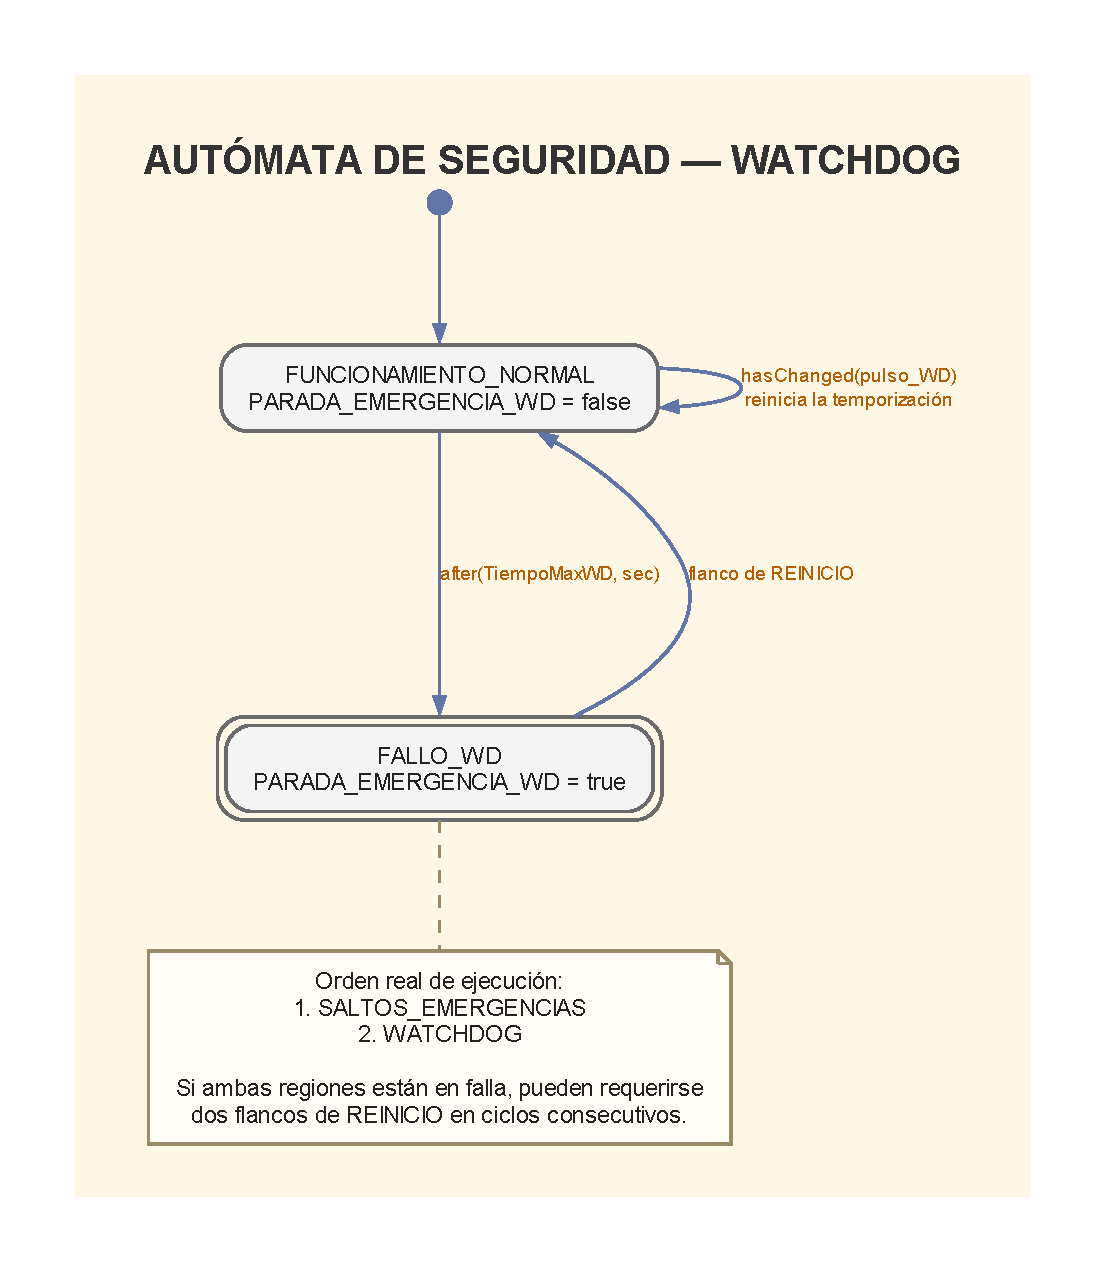
\includegraphics[height=0.70\textheight,keepaspectratio]{diagramas_automatas_revision/09_watchdog.pdf}
    \caption{Región \texttt{WATCHDOG}, temporización de actividad y recuperación mediante flanco de reinicio.}
\end{figure}


\subsection{Matriz causa--efecto}
\begin{table}[!htbp]
\centering
\caption{Respuesta del nivel de seguridad.}
\begin{tabular}{L{4.2cm} C{1.8cm} C{1.8cm} C{1.8cm} C{2.0cm} C{2.0cm}}
\toprule
Causa & Permiso global & Permiso carro & Permiso izaje & Apertura freno carro & Apertura frenos izaje\\
\midrule
Operación normal & Sí & Sí & Sí & Sí & Sí\\
Límite último horizontal & Sí & No & Sí & No & Sí\\
Límite último vertical & Sí & Sí & No & Sí & No\\
Exceso de velocidad vertical & Sí & Sí & No & Sí & No\\
Pulsador de emergencia & No & No & No & No & No\\
Falla de \textit{watchdog} & No & No & No & No & No\\
Emergencia parcial y flanco del otro eje & No & No & No & No & No\\
\bottomrule
\end{tabular}
\end{table}

\subsection{Secuencia de rearme}
El rearme de una emergencia no equivale a una orden de marcha. En una emergencia parcial, al mantenerse el permiso global, no se impone por esta causa el paso del supervisor por APAGADO; el eje no afectado conserva su autorización. Primero deben desaparecer las causas físicas que originaron la intervención. Luego el operador aplica el flanco de reinicio requerido por la región correspondiente. Al regresar el nivel de seguridad a funcionamiento normal se restablecen las autorizaciones. Después de una emergencia total, el supervisor debe completar la parada y recorrer nuevamente \texttt{APAGADO}, \texttt{ARRANQUE} y \texttt{LISTO} antes de admitir movimiento.

Cuando la emergencia total coincide con \texttt{FALLO\_WD}, el orden de ejecución de las regiones determina el comportamiento documentado: el primer flanco puede eliminar el fallo del watchdog después de que la región de emergencias ya fue evaluada. Por ello, la salida de emergencia total puede requerir un segundo flanco en una activación posterior. Esta condición se presenta como una particularidad del modelo analizado y no como una secuencia genérica de rearme.

\subsection{Aplicación final de las autorizaciones}
Las salidas del autómata de seguridad no reemplazan las órdenes del supervisor. Cada autorización se combina mediante una compuerta lógica AND con la solicitud normal de apertura correspondiente. Las órdenes operativas pueden mantenerse verdaderas durante \texttt{TB\_APLICANDO} o \texttt{HB\_APLICANDO} mientras se completa la detención; no corresponden exclusivamente a los estados \texttt{TB\_ABIERTO} y \texttt{HB\_ABIERTO}. Por tanto, el supervisor puede mantener un freno aplicado aun cuando seguridad lo autorice, pero no puede liberarlo si el nivel de seguridad lo prohíbe.

\begin{figure}[!htbp]
\centering
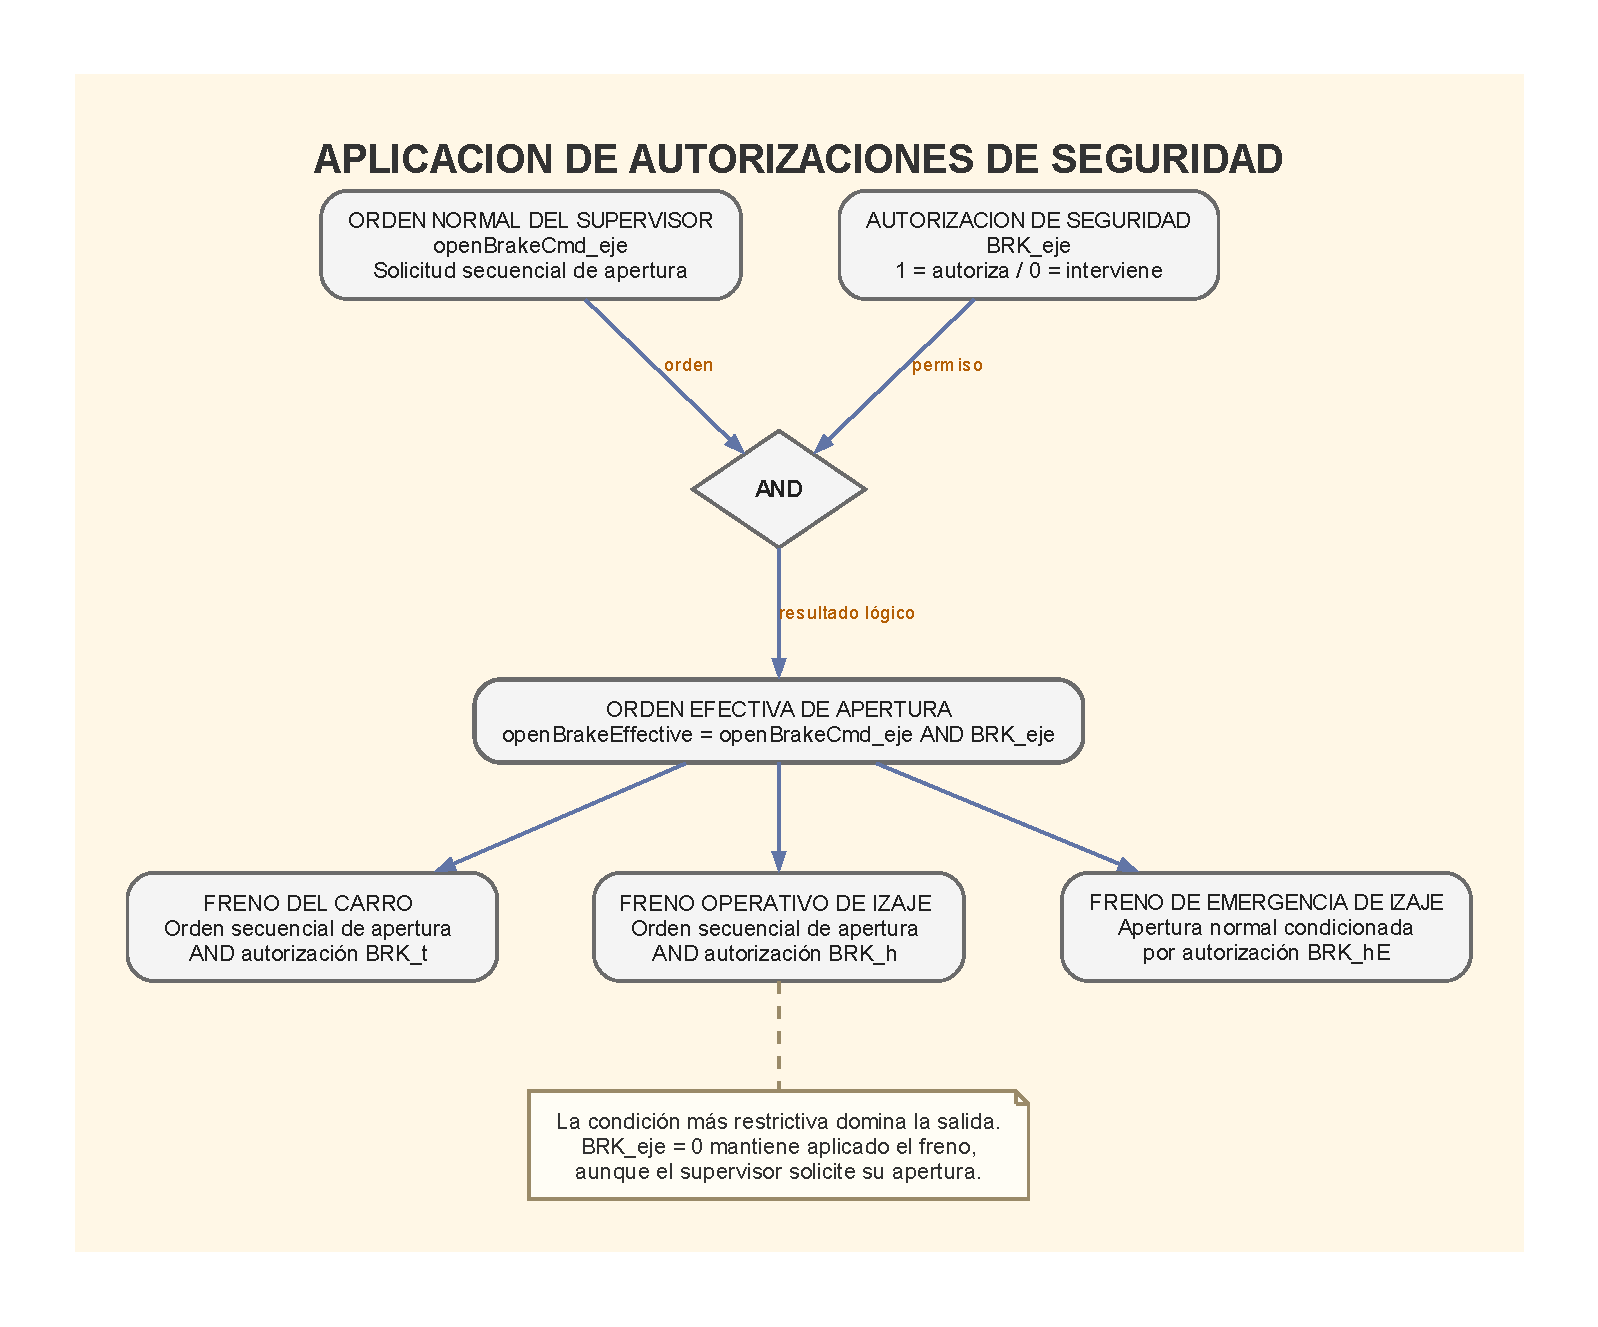
\includegraphics[width=0.98\textwidth,height=0.68\textheight,keepaspectratio]{diagramas_automatas_revision/11_compuertas_seguridad.pdf}
\caption{Combinación lógica de las órdenes del supervisor con las autorizaciones del nivel de seguridad.}
\label{fig:compuertas_seguridad_vectorial}
\end{figure}

\subsection{Particularidades de ejecución del nivel de seguridad}
La documentación del nivel de seguridad debe considerar las siguientes características específicas del Stateflow implementado:
\begin{itemize}
    \setlength{\itemsep}{0.45em}
    \item las emergencias parciales inhiben el eje afectado y conservan autorizado el eje restante;
    \item los límites últimos se reconocen mediante detección de flanco en las transiciones indicadas;
    \item \texttt{permitGlobal} permanece verdadero durante una emergencia limitada a un único eje;
    \item \texttt{SALTOS\_EMERGENCIAS} se evalúa antes que \texttt{WATCHDOG};
    \item la solicitud del watchdog es reconocida por la región de emergencias en la activación siguiente;
    \item una coincidencia de emergencia total y fallo de watchdog puede requerir dos flancos de reinicio.
\end{itemize}
Estas particularidades completan la interpretación de los diagramas y de la matriz causa--efecto sin introducir modificaciones sobre el modelo.



\subsection{Implementación manual del nivel de seguridad en CODESYS}
La versión manual distribuye protección en cinco SFC: un contenedor paralelo y cuatro monitores de carro, izaje, watchdog y emergencia total. \path{PRG_PRESEGURIDAD} calcula los flancos y la temporización; \path{PRG_SALIDAS_SEGURIDAD} arbitra las autorizaciones y permisos. Estos programas se ejecutan antes del supervisor en \path{MainTask_20ms}.

La secuencia exacta es: enlace OPC UA, preseguridad, SFC de carro, SFC de izaje, SFC de watchdog, SFC total, contenedor paralelo y salidas de seguridad. Los cuatro monitores se llaman en cada ciclo, independientemente de las acciones del contenedor. \path{SFC_AUTOMATA_SEGURIDAD} mantiene sus dos pasos de región porque la transición posterior a la convergencia tiene condición \texttt{FALSE}; su representación expresa paralelismo, pero no selecciona por sí misma las salidas de emergencia.

\begin{figure}[!htbp]
\centering
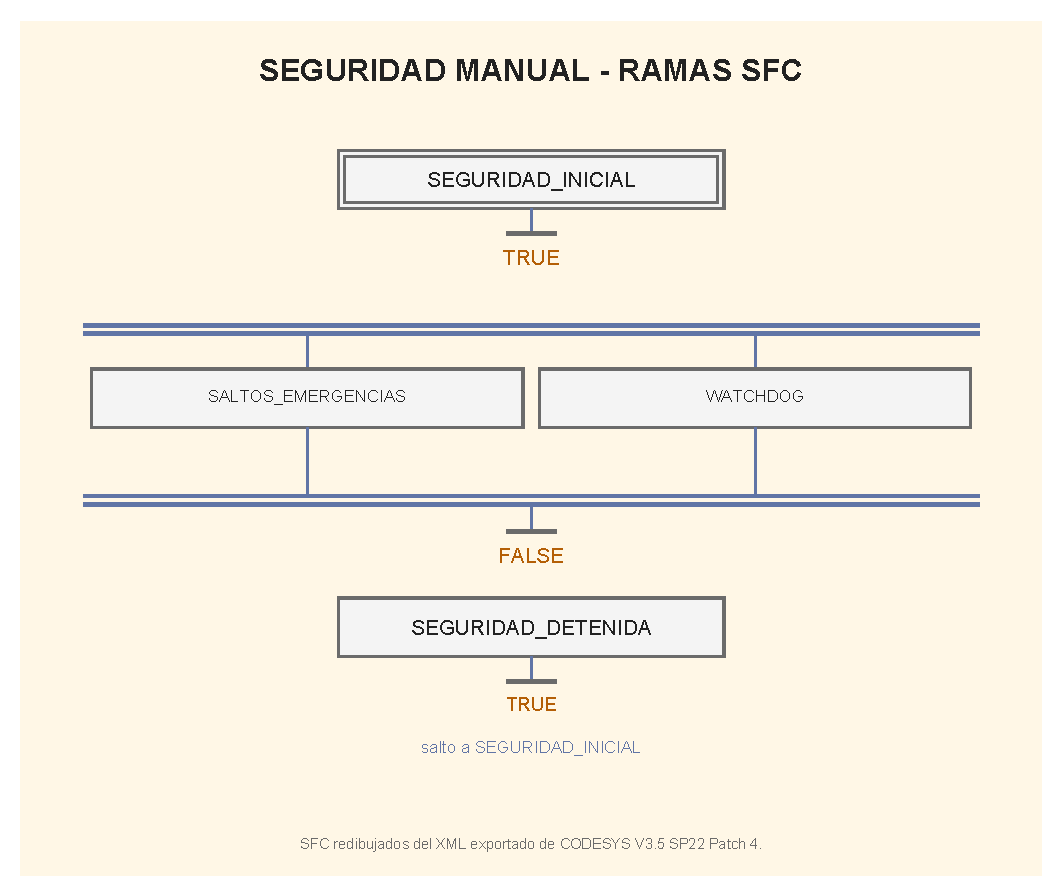
\includegraphics[width=0.96\textwidth]{diagramas_codesys_manual/18_sfc_seguridad_paralela.pdf}
\caption{Contenedor SFC paralelo del nivel de seguridad manual. Los SFC de detección y el arbitraje de salidas se ejecutan mediante llamadas separadas de la tarea.}
\label{fig:sfc_seg_paralela}
\end{figure}


\subsection{SFC de emergencias parciales por eje}
\path{SFC_SEG_CARRO} posee los pasos \texttt{CARRO\_SEGURO} y \texttt{EMERGENCIA\_CARRO}; \path{SFC_SEG_IZAJE} posee \texttt{IZAJE\_SEGURO} y \texttt{EMERGENCIA\_IZAJE}. Los flancos de límites últimos y sobrevelocidad proceden del preprocesamiento. El rearme de cada monitor exige flanco de reinicio y desaparición de los sensores de su propio eje.

Los monitores pueden quedar activos simultáneamente. Así se reconocen los flancos de ambos ejes en la misma llamada de tarea, y el monitor total y el arbitraje pueden producir inhibición total. Esta organización difiere de las transiciones alternativas ordenadas desde el único estado normal de Stateflow. Los monitores parciales no comprueban el pulsador de emergencia en su guarda de recuperación; su efecto se conserva mediante el monitor total y el arbitraje final.

\begin{figure}[!htbp]
\centering
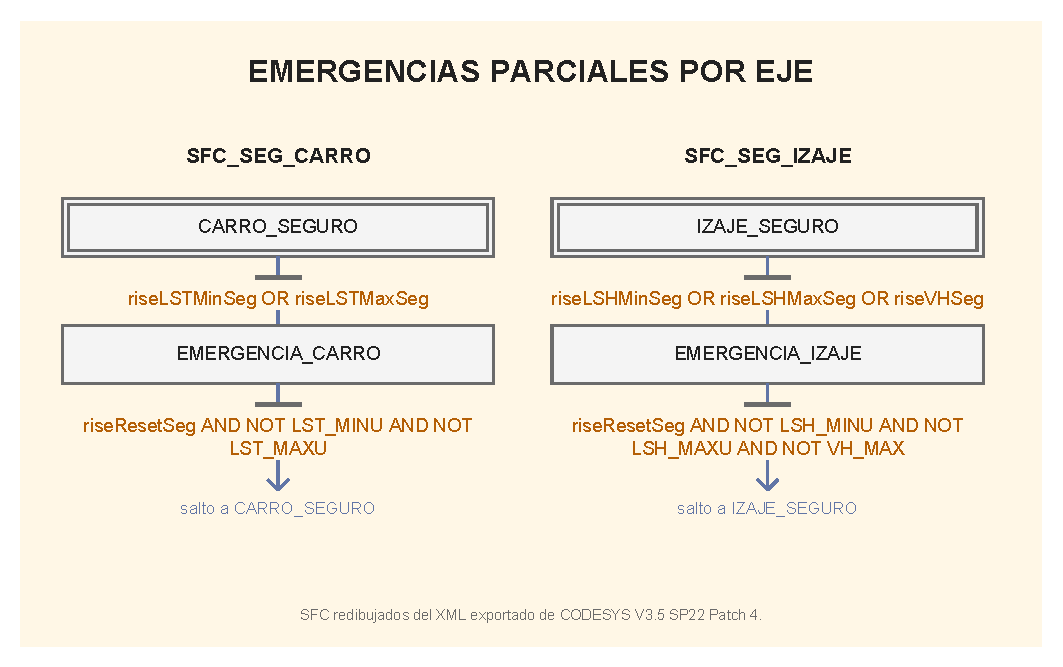
\includegraphics[width=0.98\textwidth]{diagramas_codesys_manual/19_sfc_seguridad_ejes.pdf}
\caption{Monitores SFC independientes de emergencia del carro y del izaje, con sus condiciones exactas de disparo y rearme.}
\label{fig:sfc_seg_ejes}
\end{figure}


\subsection{SFC de watchdog y emergencia total}
El preprocesador compara \texttt{pulso\_WD} con su valor anterior. Ante cambio pone a cero el acumulador; de lo contrario suma $0.02~\mathrm{s}$. \path{SFC_SEG_WATCHDOG} pasa a disparado cuando el acumulador alcanza $\max(0.02,\allowbreak\texttt{TiempoMaxWD})$. Su retorno exige reinicio y desaparición del timeout. En el archivo del proyecto, el valor inicial de \texttt{TiempoMaxWD} es $5~\mathrm{s}$. El watchdog de la tarea, configurado a $100~\mathrm{ms}$, es un mecanismo diferente y no debe confundirse con esta vigilancia del pulso.

\path{SFC_SEG_TOTAL} detecta pulsador, falla OPC UA, watchdog disparado o coexistencia de emergencias de ambos ejes. Su recuperación exige reinicio y ausencia de todas esas condiciones. El watchdog se ejecuta antes del SFC total, por lo que su nuevo paso puede ser consumido por el monitor total dentro de la misma llamada de tarea. También pueden limpiarse los monitores antes de evaluar el rearme total si todas sus guardas son verdaderas; no se traslada automáticamente a esta implementación la particularidad de dos flancos del chart.

La falla de comunicación se obtiene en \path{PRG_ENLACE_OPCUA} por ausencia de cambios del latido de Simulink. \texttt{opcTimeoutSeconds} se inicializa a $1~\mathrm{s}$ en el proyecto; puede configurarse para el ensayo. Estos valores describen el archivo exportado, no una lectura de parámetros activos del runtime. La vigilancia de comunicación es una protección adicional necesaria para esta arquitectura repartida entre PLC y Simulink.

\begin{figure}[!htbp]
\centering
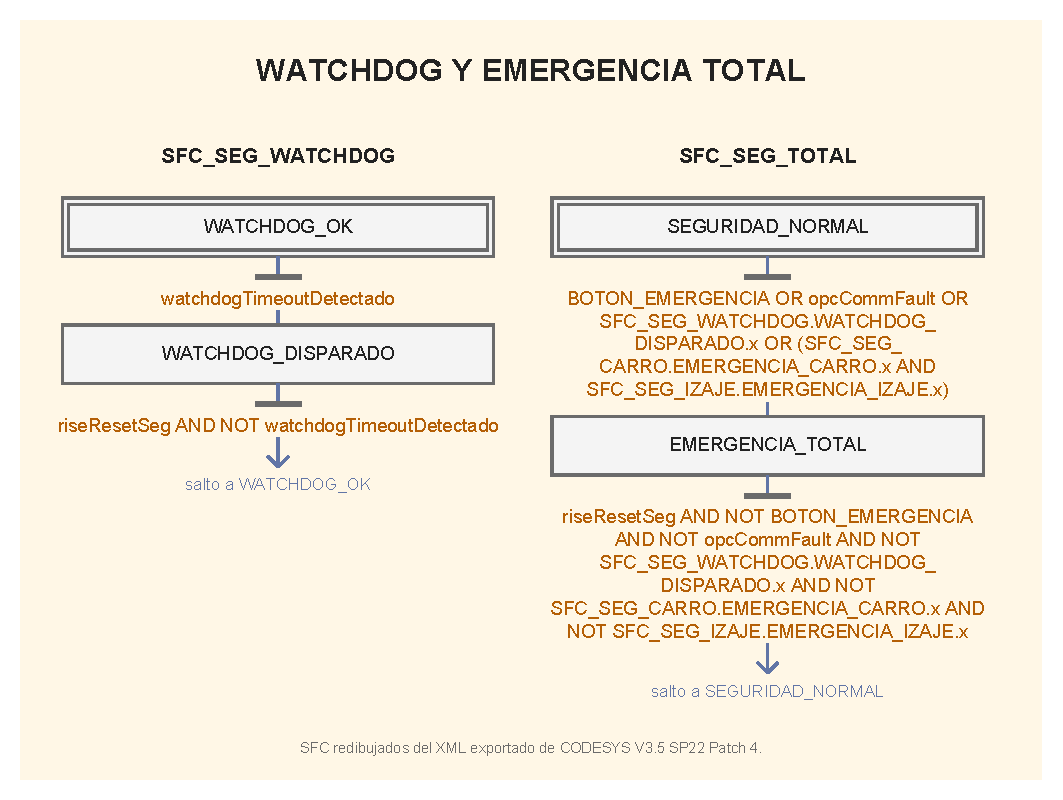
\includegraphics[width=0.98\textwidth]{diagramas_codesys_manual/20_sfc_watchdog_total.pdf}
\caption{SFC de watchdog y emergencia total. La comunicación OPC UA interviene explícitamente en disparo y recuperación.}
\label{fig:sfc_wd_total}
\end{figure}


\subsection{Comparación de seguridad: Stateflow y CODESYS manual}
El arbitraje ST utiliza prioridad total, coincidencia de parciales, izaje, carro y normal. Mantiene la polaridad activa en uno de \texttt{BRK\_t}, \texttt{BRK\_h} y \texttt{BRK\_hE}, pero transforma sus permisos de manera diferente al subsistema Stateflow:
\begin{align}
\texttt{safetyPermitGlobal}&=\neg\texttt{EMERGENCIA}\notag\\
&\quad\land\neg\texttt{PARADA\_EMERGENCIA\_WD}\land\neg\texttt{opcCommFault},\\
\texttt{safetyPermitTrolley}&=\texttt{safetyPermitGlobal}\land\texttt{BRK\_t},\\
\texttt{safetyPermitHoist}&=\texttt{safetyPermitGlobal}\land\texttt{BRK\_h}\land\texttt{BRK\_hE}.
\end{align}
En consecuencia, una emergencia parcial anula el permiso global y ambos permisos de movimiento en CODESYS manual, aun cuando la autorización de freno del eje no afectado permanezca verdadera. El programa final del supervisor fuerza además las órdenes de apertura a falso cuando falta el permiso global. No corresponde aplicar a esta versión la matriz del Stateflow, cuyo permiso global se calcula con OR de las autorizaciones de eje.

\begin{table}[!htbp]
\centering\small
\caption{Permisos efectivos: diferencia ante emergencias parciales.}\label{tab:permisos_sfc_vs_sf}
\begin{tabular}{L{4.0cm} C{1.3cm} C{1.3cm} C{1.3cm} C{1.3cm} C{1.3cm} C{1.3cm}}
\toprule
& \multicolumn{3}{c}{Stateflow} & \multicolumn{3}{c}{CODESYS manual}\\
Condición & Global & Carro & Izaje & Global & Carro & Izaje\\
\midrule
Normal & 1 & 1 & 1 & 1 & 1 & 1\\
Emergencia de carro & 1 & 0 & 1 & 0 & 0 & 0\\
Emergencia de izaje & 1 & 1 & 0 & 0 & 0 & 0\\
Emergencia total & 0 & 0 & 0 & 0 & 0 & 0\\
\bottomrule
\end{tabular}
\end{table}

{\footnotesize
\begin{longtable}{L{3.0cm} L{5.8cm} L{5.8cm}}
\caption{Diferencias de estructura y ejecución del nivel de seguridad.}\label{tab:comparacion_seg_sfc}\\
\toprule Aspecto & Stateflow de referencia & CODESYS manual SFC\\\midrule
\endfirsthead
\toprule Aspecto & Stateflow de referencia & CODESYS manual SFC\\\midrule
\endhead
Estados & Región de emergencia con cuatro estados exclusivos y watchdog con dos estados. & Cuatro monitores independientes de dos pasos y un contenedor paralelo.\\
Simultaneidad de ejes & Prioridad de transición: total, izaje, carro; puede consumir sólo uno de los flancos desde normal. & Ambos monitores reconocen sus flancos en la misma tarea; la coincidencia genera total.\\
Emergencia parcial & Mantiene permiso global y el eje no afectado autorizado. & Anula permiso global y ambos movimientos.\\
Pérdida de comunicación & No integra una entrada OPC UA al chart de referencia. & \texttt{opcCommFault} provoca total y mantiene permisos inhibidos.\\
Watchdog & Emergencias antes de watchdog; reconocimiento de su solicitud en activación siguiente. & Watchdog antes de total y salidas; consumo del nuevo paso dentro de la tarea.\\
Rearme watchdog & Flanco de reinicio como guarda de salida del fallo. & Flanco de reinicio y timeout inactivo.\\
Cambio en el vencimiento & Transición por vencimiento se evalúa antes de realimentar por cambio. & Preprocesador reinicia el acumulador ante cambio antes de evaluar timeout.\\
Acciones de protección & Asignadas en la entrada de cada estado del chart. & Calculadas cada llamada en ST a partir de pasos activos y comunicación.\\
\bottomrule
\end{longtable}}

La comparación se fundamenta en el XML y los programas ST exportados. Describe las diferencias de arquitectura y comportamiento encontradas en el simulador; no se presupone equivalencia completa con el chart.



\subsection{Implementación automática de protección en ST}
La protección se generó separadamente desde \path{Nivel 0 - Seguridad/Automata de proteccion} de la misma copia Stateflow. La comparación previa registró ocho estados jerárquicos, trece transiciones y catorce datos, sin funciones MATLAB internas. PLC Coder produjo el bloque principal y dos auxiliares, que se integraron con prefijo \texttt{SEG\_} y el nombre \path{FB_GEN_SEGURIDAD}. \path{PRG_AUTO_SEGURIDAD} conecta las nueve entradas y cinco salidas originales del chart, inicializa la instancia una vez y luego ejecuta su STEP antes del supervisor.

El código ST conserva la región de emergencias de estados exclusivos y la región watchdog, las memorias anterior y actual para detección de cambios y las prioridades de transición del chart. El watchdog temporal utiliza un bloque IEC \texttt{Standard.TON}. Por tanto, su tiempo corresponde al runtime PLC y no al tiempo acelerado de la planta Simulink. Las máquinas de estados de las Figuras de Stateflow anteriores siguen siendo la representación de este núcleo generado; los cinco SFC manuales representan una traducción diferente.

Esta conservación incluye el orden de ejecución de regiones del chart: emergencia precede a watchdog. Una solicitud de watchdog producida después de evaluar emergencias es consumida por esa región en la siguiente activación. No se sustituye por el orden de los monitores manuales, donde watchdog se llama antes del SFC total. Igualmente, la prioridad entre transiciones alternativas desde normal se conserva en ST; no se convierte en dos monitores independientes que reconocen ambos flancos en paralelo.

\subsection{Diferencias entre protección generada y permisos de integración}
Las salidas \texttt{BRK\_t}, \texttt{BRK\_h} y \texttt{BRK\_hE}, \texttt{EMERGENCIA} y \texttt{PARADA\_EMERGENCIA\_WD} proceden del bloque generado. Los permisos efectivos se calculan después en el adaptador, con las mismas expresiones de la implementación manual de la Sección anterior: permiso global exige ausencia de emergencia, watchdog y falla OPC UA; los permisos de cada eje se combinan con ese global y sus autorizaciones de freno.

En consecuencia, aunque el núcleo generado conserve una emergencia parcial con autorización de freno del eje no afectado, el adaptador anula el permiso global y ambos movimientos. Esta diferencia respecto del permiso global OR de Stateflow no es un error de generación: se introdujo expresamente en la capa de integración. La matriz de permisos de CODESYS manual también describe estos permisos efectivos de la versión automática. No debe afirmarse equivalencia de las salidas finales de toda la aplicación sólo porque las transiciones del bloque procedan del mismo chart.

La pérdida de comunicación tampoco se añade como entrada a la máquina de emergencia generada: \texttt{opcCommFault} inhibe directamente los permisos en el adaptador. En la versión manual, además de inhibir permisos, esa señal es una guarda del SFC de emergencia total. Así, una misma inhibición física puede estar representada por estados internos distintos. Las compuertas finales del supervisor generado impiden habilitar reguladores o abrir frenos cuando esos permisos faltan.

\begin{table}[!htbp]
\centering\footnotesize
\caption{Protección: núcleo generado y adaptación de la aplicación.}\label{tab:seguridad_auto_capas}
\begin{tabular}{L{3.6cm} L{5.5cm} L{5.5cm}}
\toprule
Aspecto & ST generado desde Stateflow & Integración CODESYS\\
\midrule
Emergencias & Estados exclusivos, guardas y prioridad de la referencia. & Permiso global anulado también ante emergencia parcial.\\
Watchdog & Región después de emergencias; temporizador IEC TON. & Tipo Standard.TON y ejecución desde tarea de 20 ms.\\
Comunicación & No agrega una entrada OPC UA al chart. & Falla OPC UA inhibe directamente permisos.\\
Rearme & Conserva flancos y guardas del chart. & Reset de HMI no reinicializa toda la memoria del supervisor.\\
Precarga de ensayo & Bloque de protección sin cambios para medio ciclo. & Extensión de perfil sólo en supervisor y banco de ensayo.\\
\bottomrule
\end{tabular}
\end{table}

Las corridas disponibles comprobaron ausencia de fallas y emergencias durante la maniobra realizada; no ejercitaron todas las combinaciones de límites, pulsador, watchdog y rearme. La comparación aquí presentada distingue el análisis del código, la compilación registrada y la evidencia dinámica de medio ciclo.


\section{Visualización HMI}
La visualización representa la grúa, el carro, el cable, el \textit{spreader}, los contenedores, el muelle, el barco, el perfil relevado y la línea de seguridad. Los tensores diagonales internos de la estructura fueron eliminados para conservar únicamente pilares y vigas horizontales, obteniendo una representación más clara.

El HMI permite emitir órdenes de marcha, parada, reinicio, barrido, modo automático, inicio automático, selección de anti-sway y accionamiento de \textit{twistlocks}. También muestra el código de modo, estado de carga, validez del perfil, alarmas, fallas y permisos de seguridad.

La representación del contenedor tomado se realiza sin líneas verticales superpuestas. La posición gráfica se calcula con las coordenadas de la carga y no con la posición del carro, de manera que el balanceo se observa correctamente.

% IMAGEN A INSERTAR: captura completa del HMI final corregido.
\figplaceholder[0.58\textheight]{Captura completa de la visualización final durante un traslado, con panel de mando y línea de seguridad.}{Interfaz HMI integrada al modelo.}


\section{Pruebas de simulación}
\subsection{Prueba ciclo completo en simulink}

Se ensayó en una única corrida el relevamiento LiDAR y dos transferencias consecutivas en sentidos opuestos. La planta, el controlador de movimiento, el supervisor y el nivel de seguridad se ejecutaron íntegramente en Simulink. Un operador programado accionó los controles reales de la HMI, sin forzar estados ni sustituir las decisiones de los autómatas.

La primera transferencia llevó un contenedor del centro del muelle, \textit{slot} 6 ($x=-16.58~\mathrm{m}$), al centro del barco, \textit{slot} 23 ($x=24.90~\mathrm{m}$). Después se desplazó el conjunto vacío al extremo derecho operable del barco, \textit{slot} 32 ($x=46.86~\mathrm{m}$), y se trasladó otro contenedor al extremo izquierdo del muelle, \textit{slot} 1 ($x=-28.78~\mathrm{m}$). La duración total fue de $626.36~\mathrm{s}$.

Los posicionamientos se solicitaron en automático. Las tomas, aproximaciones finales de apoyo y extracciones verticales se realizaron mediante los mandos proporcionales de la HMI, respetando los permisos y retenciones del supervisor. El controlador antisway conservó su realimentación angular, su anticipación limitada y su rampa de habilitación.

\subsection{Cronología de las dos transferencias}

\begin{longtable}{C{1.6cm} C{1.0cm} L{6.4cm} L{4.4cm}}

\caption{Eventos efectivos de la Prueba ciclo completo en simulink.}\label{tab:cronologia_prueba_ciclo_completo_en_simulink}\\

\toprule Tiempo [s] & Tramo & Evento & Destino\\\midrule\endfirsthead

\toprule Tiempo [s] & Tramo & Evento & Destino\\\midrule\endhead

$0.24$ & 1 & Arranque & Toma en muelle\\

$0.40$ & 1 & Inicio del barrido & Toma en muelle\\

$114.64$ & 1 & Extracción y despeje local & Toma en muelle\\

$116.68$ & 1 & Solicitud de posicionamiento automático & Toma en muelle\\

$116.76$ & 1 & Posicionamiento automático efectivo & Toma en muelle\\

$138.88$ & 1 & Solicitud de aproximación final manual & Toma en muelle\\

$142.84$ & 1 & Descenso final & Toma en muelle\\

$192.12$ & 1 & Contacto y solicitud de twistlocks & Toma en muelle\\

$193.16$ & 2 & Extracción y despeje local & Entrega en barco\\

$194.96$ & 1 & Toma física confirmada & Toma en muelle\\

$206.80$ & 2 & Solicitud de posicionamiento automático & Entrega en barco\\

$206.88$ & 2 & Posicionamiento automático efectivo & Entrega en barco\\

$270.84$ & 2 & Solicitud de aproximación final manual & Entrega en barco\\

$273.24$ & 2 & Descenso final & Entrega en barco\\

$308.60$ & 2 & Contacto y solicitud de twistlocks & Entrega en barco\\

$309.00$ & 3 & Extracción y despeje local & Toma en barco\\

$309.00$ & 2 & Entrega física confirmada & Entrega en barco\\

$347.88$ & 3 & Solicitud de posicionamiento automático & Toma en barco\\

$347.96$ & 3 & Posicionamiento automático efectivo & Toma en barco\\

$375.92$ & 3 & Solicitud de aproximación final manual & Toma en barco\\

$379.52$ & 3 & Descenso final & Toma en barco\\

$444.72$ & 3 & Contacto y solicitud de twistlocks & Toma en barco\\

$445.76$ & 4 & Extracción y despeje local & Entrega en muelle\\

$447.56$ & 3 & Toma física confirmada & Toma en barco\\

$510.88$ & 4 & Solicitud de posicionamiento automático & Entrega en muelle\\

$510.96$ & 4 & Posicionamiento automático efectivo & Entrega en muelle\\

$612.88$ & 4 & Solicitud de aproximación final manual & Entrega en muelle\\

$615.28$ & 4 & Descenso final & Entrega en muelle\\

$623.88$ & 4 & Contacto y solicitud de twistlocks & Entrega en muelle\\

$624.32$ & 4 & Entrega física confirmada & Entrega en muelle\\

$624.32$ & 4 & Parada final & Entrega en muelle\\

\bottomrule\end{longtable}

\subsection{Relevamiento y actualización del perfil}

El barrido precedió a ambas tomas. La comparación del perfil relevado con el perfil físico inicial de los slots operables produjo un error máximo de $0.000000~\mathrm{m}$. Los slots no operables se excluyen de esa métrica, porque su cota neutra no representa una superficie de toma o entrega.

El perfil final conserva el balance de los dos contenedores: disminuye $2.59~\mathrm{m}$ en los slots 6 y 32 y aumenta la misma altura en los slots 23 y 1. La comparación entre perfil inicial, perfil relevado y perfil físico final permite distinguir la medición inicial de las modificaciones posteriores debidas a las transferencias.

\begin{figure}[!htbp]
\centering
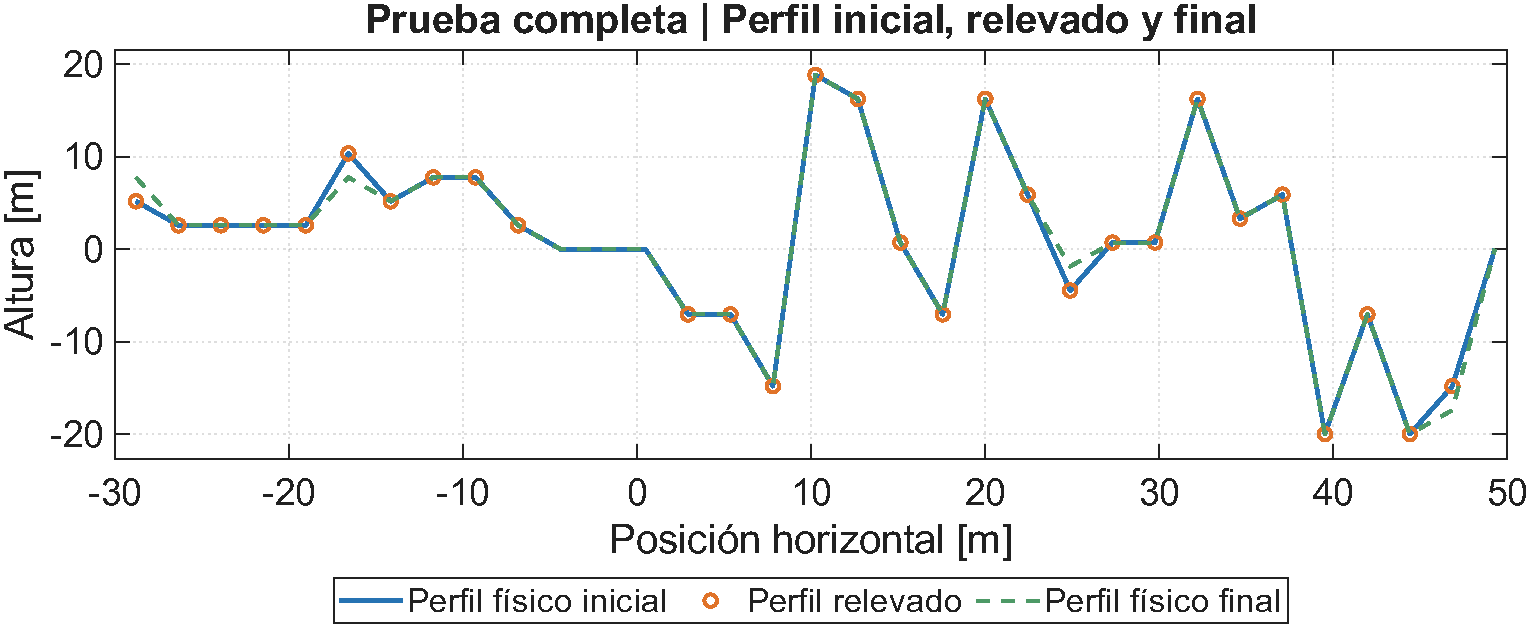
\includegraphics[width=0.98\textwidth]{resultados_prueba_ciclo_completo_en_simulink/perfil.pdf}
\caption{Perfil físico inicial, perfil relevado por LiDAR y perfil físico final después de las dos entregas.}
\label{fig:prueba_ciclo_completo_en_simulink_perfil}
\end{figure}


\begin{figure}[!htbp]
\centering
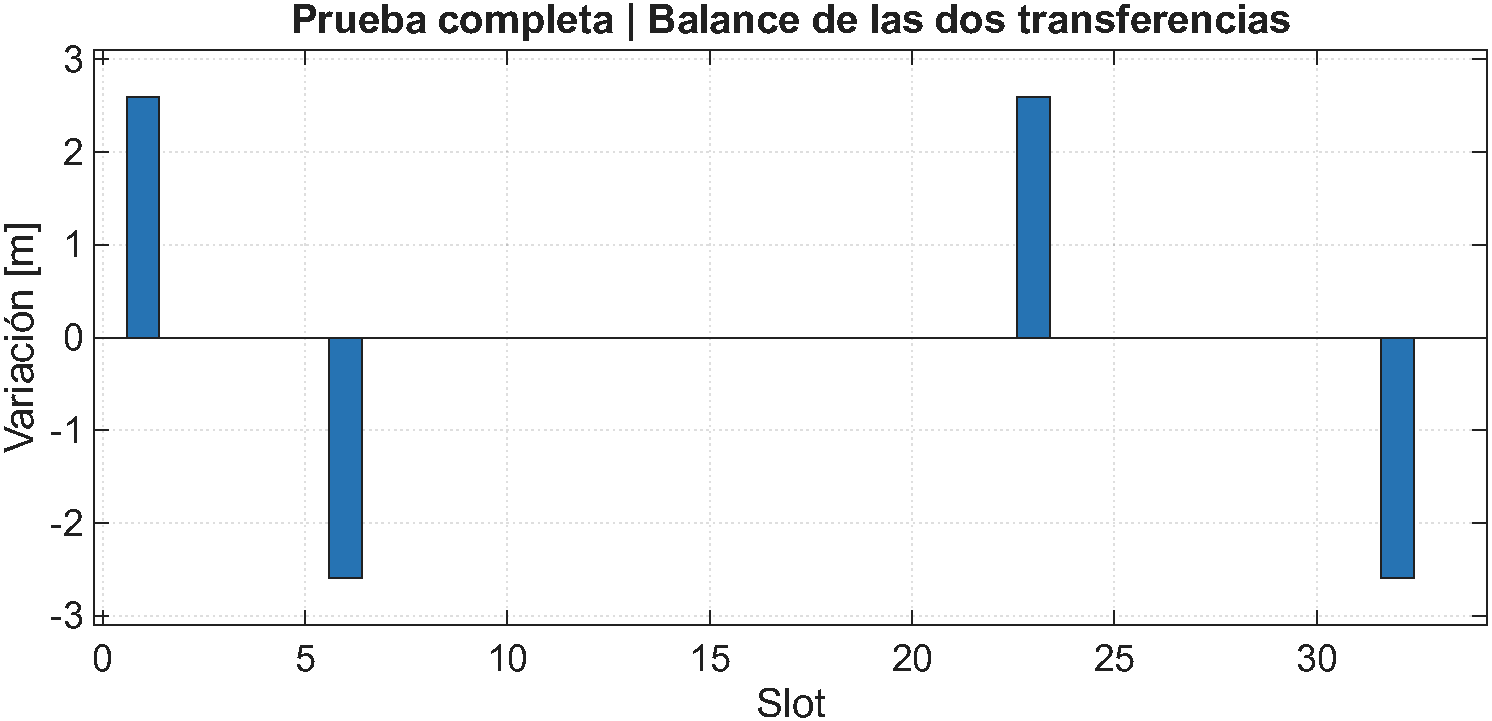
\includegraphics[width=0.98\textwidth]{resultados_prueba_ciclo_completo_en_simulink/balance_perfil.pdf}
\caption{Variación física por slot al finalizar las dos transferencias.}
\label{fig:prueba_ciclo_completo_en_simulink_balance_perfil}
\end{figure}


\begin{figure}[!htbp]
\centering
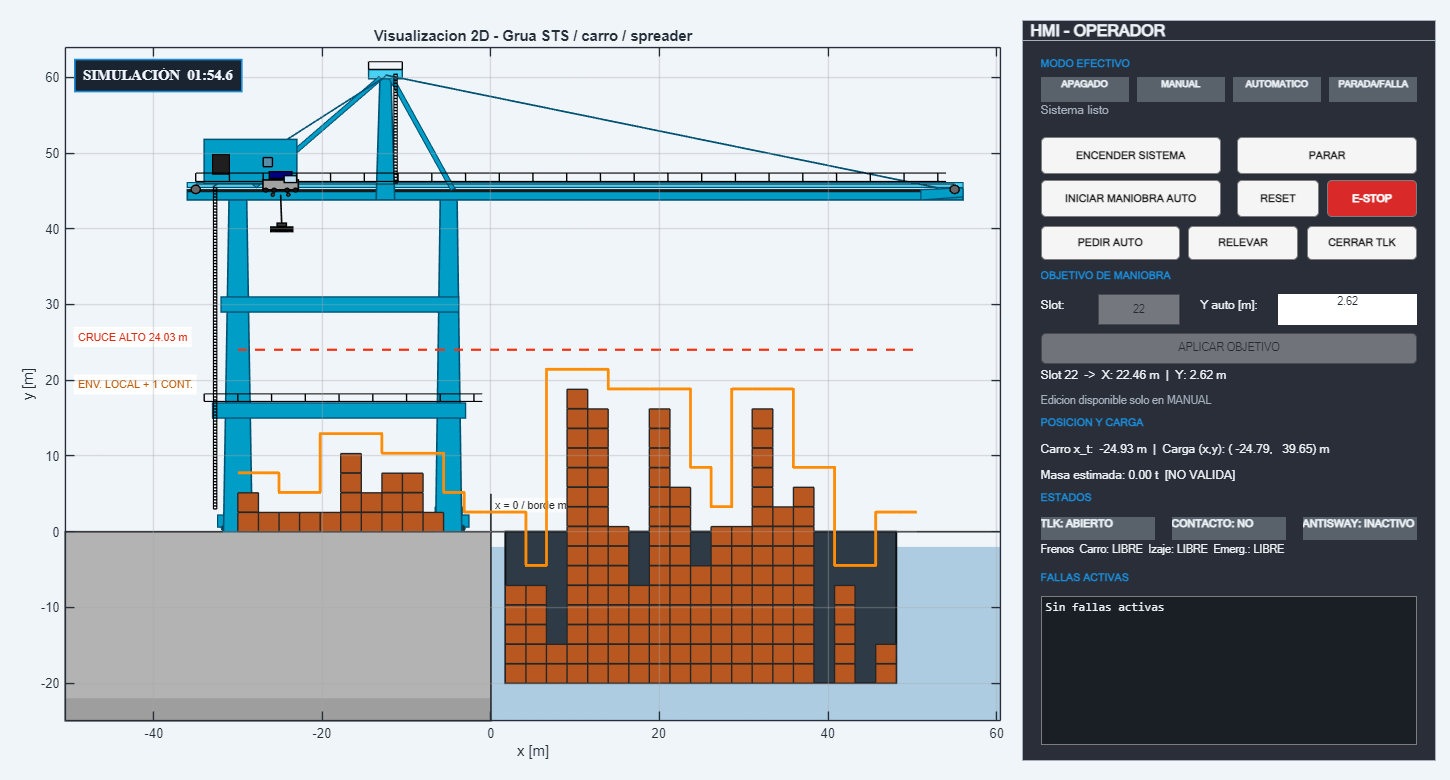
\includegraphics[width=0.98\textwidth]{resultados_prueba_ciclo_completo_en_simulink/01_barrido.png}
\caption{Visualización y HMI al finalizar el barrido real.}
\label{fig:prueba_ciclo_completo_en_simulink_01_barrido}
\end{figure}


\subsection{Dinámica del carro y seguimiento horizontal}

El recorrido horizontal cambia de sentido entre las dos entregas. Las fases vacías enlazan el fin del barrido con la primera toma y la primera entrega con la segunda toma. Las figuras representan cada magnitud en un eje independiente y comparan las referencias con las variables físicas.

La velocidad física máxima absoluta del carro en toda la corrida fue de $2.355~\mathrm{m/s}$. El máximo absoluto de aceleración física fue de $0.863~\mathrm{m/s^2}$. Estos extremos incluyen arranque, relevamiento y transitorios; no equivalen a límites de las consignas.

\begin{figure}[!htbp]
\centering
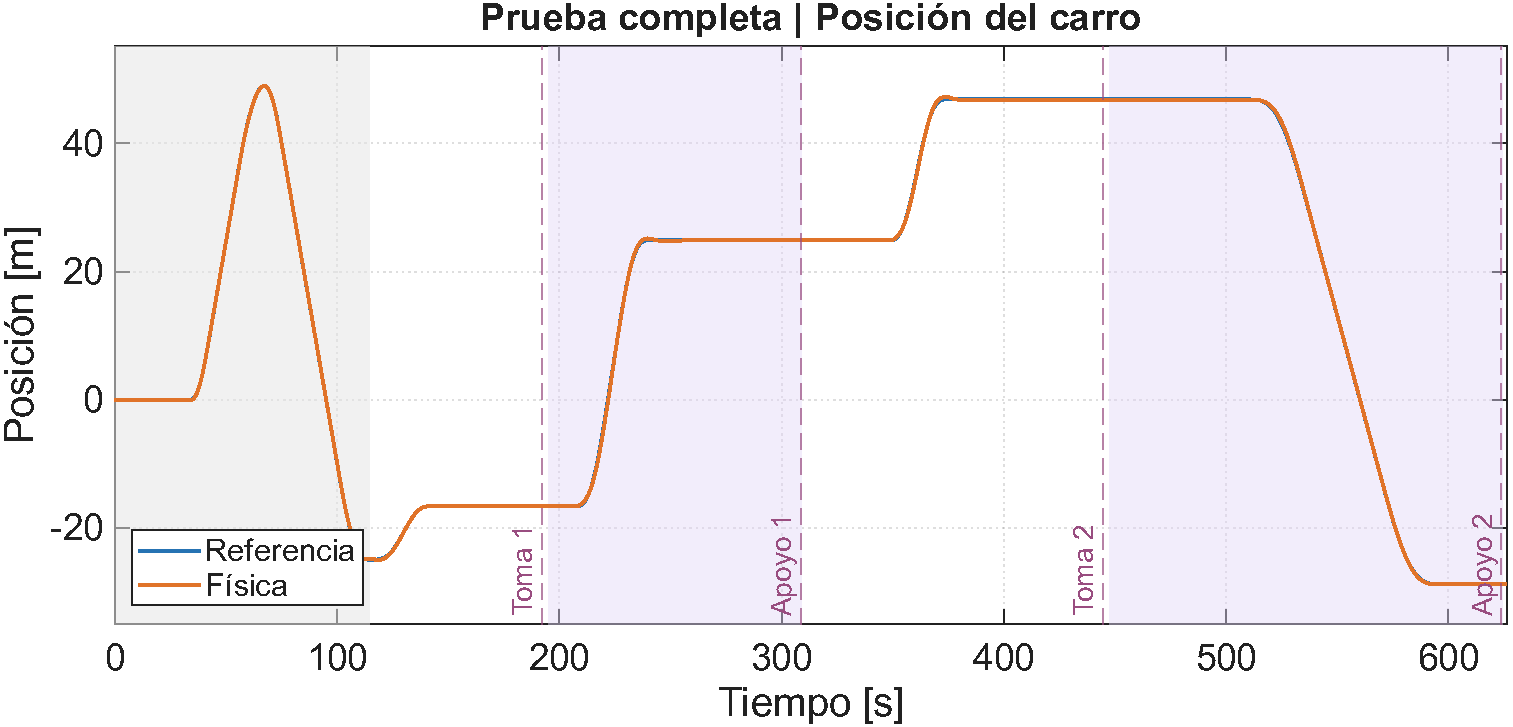
\includegraphics[width=0.98\textwidth]{resultados_prueba_ciclo_completo_en_simulink/x.pdf}
\caption{Posición horizontal del carro y referencia durante todo el ensayo.}
\label{fig:prueba_ciclo_completo_en_simulink_x}
\end{figure}


\begin{figure}[!htbp]
\centering
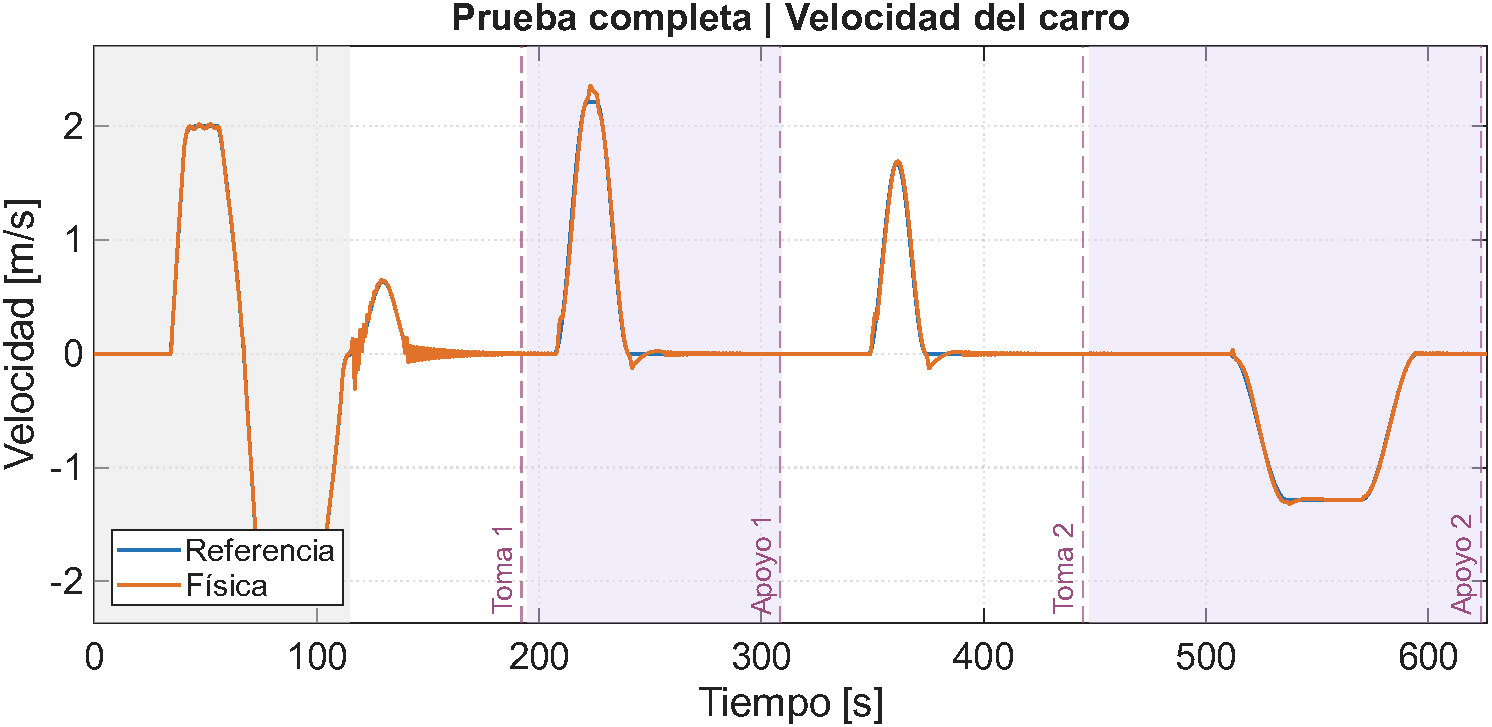
\includegraphics[width=0.98\textwidth]{resultados_prueba_ciclo_completo_en_simulink/vx.pdf}
\caption{Velocidad física del carro y referencia.}
\label{fig:prueba_ciclo_completo_en_simulink_vx}
\end{figure}


\begin{figure}[!htbp]
\centering
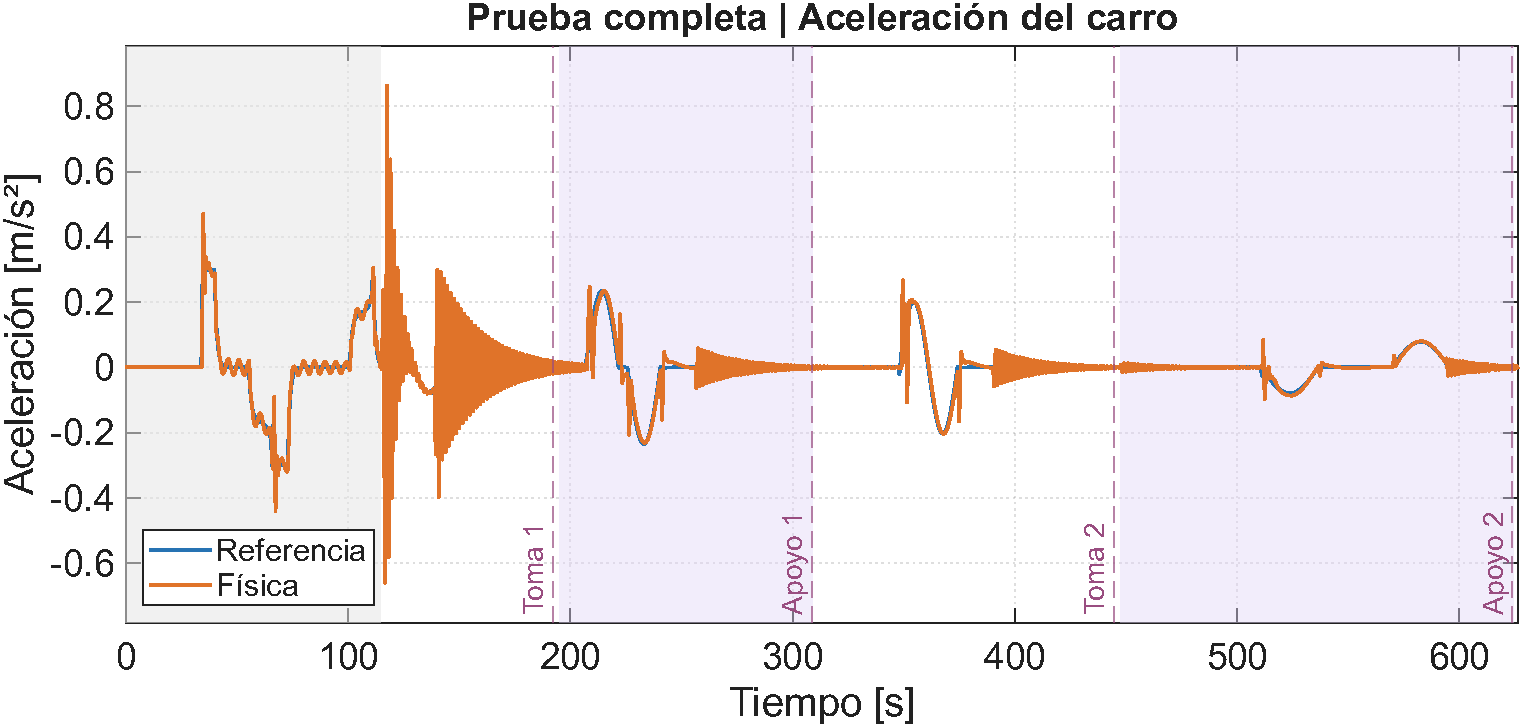
\includegraphics[width=0.98\textwidth]{resultados_prueba_ciclo_completo_en_simulink/ax.pdf}
\caption{Aceleración física del carro y referencia.}
\label{fig:prueba_ciclo_completo_en_simulink_ax}
\end{figure}


\begin{figure}[!htbp]
\centering
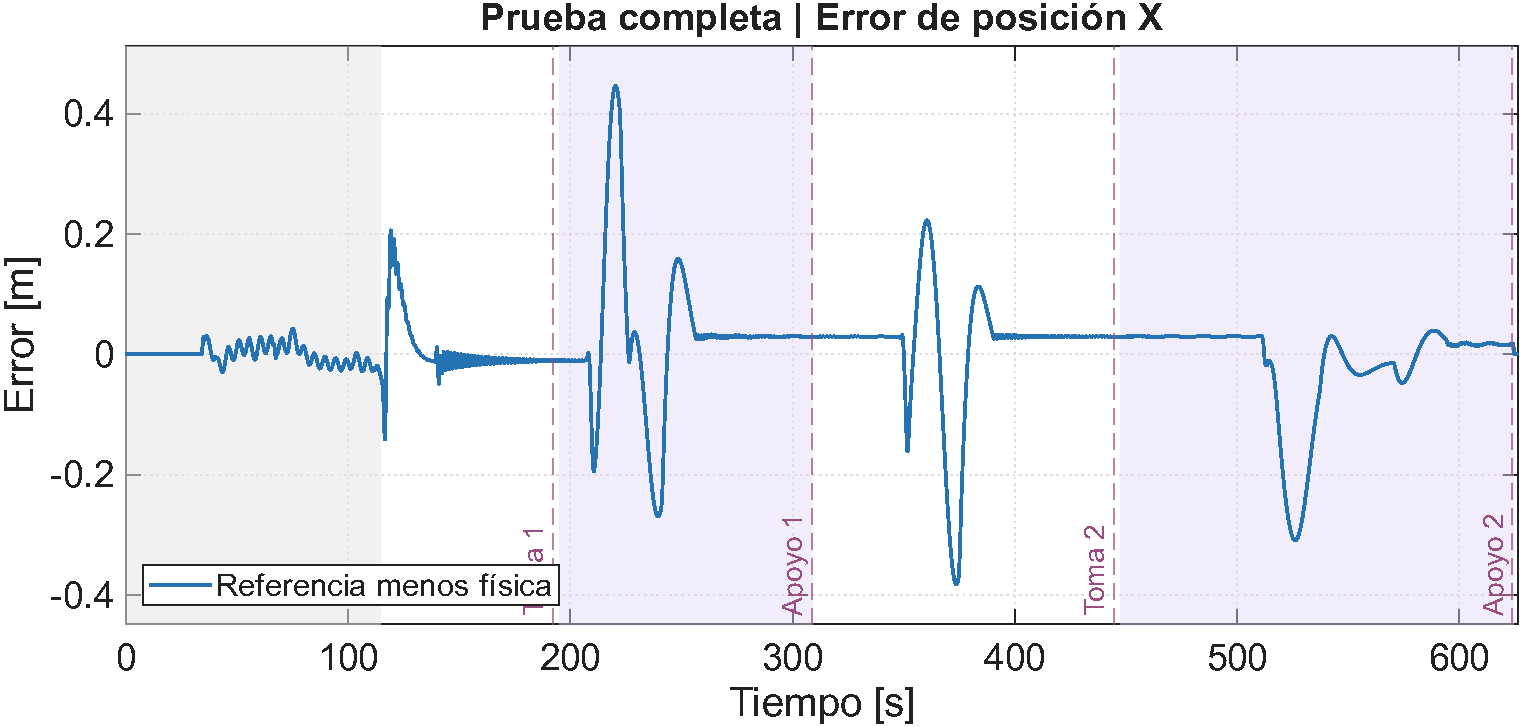
\includegraphics[width=0.98\textwidth]{resultados_prueba_ciclo_completo_en_simulink/error_x.pdf}
\caption{Error horizontal de posición, calculado como referencia menos posición física.}
\label{fig:prueba_ciclo_completo_en_simulink_error_x}
\end{figure}


\begin{figure}[!htbp]
\centering
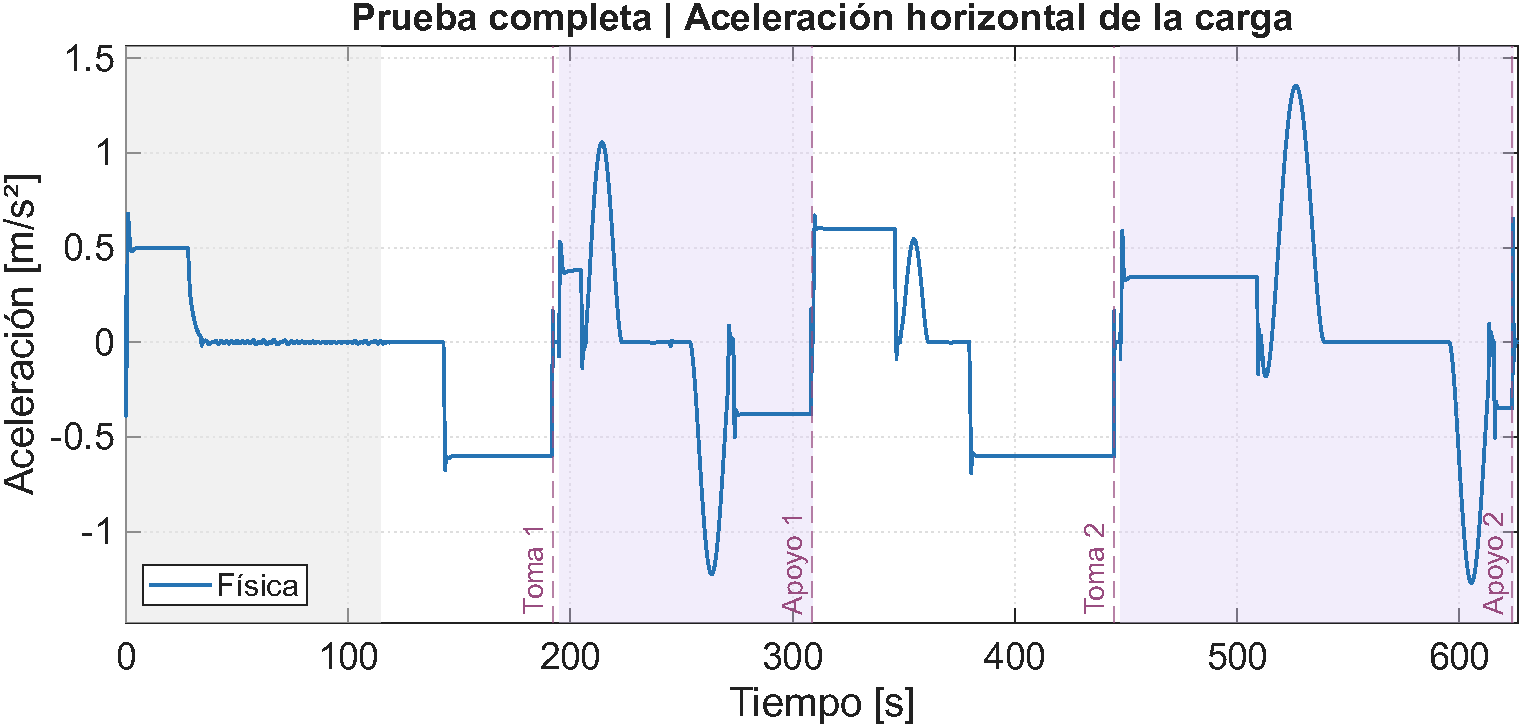
\includegraphics[width=0.98\textwidth]{resultados_prueba_ciclo_completo_en_simulink/ax_carga.pdf}
\caption{Aceleración horizontal física de la carga suspendida.}
\label{fig:prueba_ciclo_completo_en_simulink_ax_carga}
\end{figure}


\subsection{Izaje, contacto y entrega física}

Los apoyos de las dos entregas se registraron a los $308.60~\mathrm{s}$ y $623.88~\mathrm{s}$. La apertura de twistlocks se verificó junto con la liberación física y la actualización del perfil, en lugar de considerar suficiente un cambio lógico aislado.

La altura y la velocidad muestran las extracciones, el transporte y los descensos de aproximación. La aceleración de izaje se presenta en escala completa y, por separado, con un zoom vertical de $\pm1~\mathrm{m/s^2}$. El zoom permite observar la evolución entre transitorios; no elimina ni filtra los picos, que permanecen en la figura de escala completa.

El máximo absoluto de aceleración física de izaje fue de $149.77~\mathrm{m/s^2}$, a los $624.04~\mathrm{s}$. Este extremo coincide temporalmente con el transitorio del último apoyo y la apertura de twistlocks; no representa una aceleración sostenida ni el límite de la referencia.

\begin{figure}[!htbp]
\centering
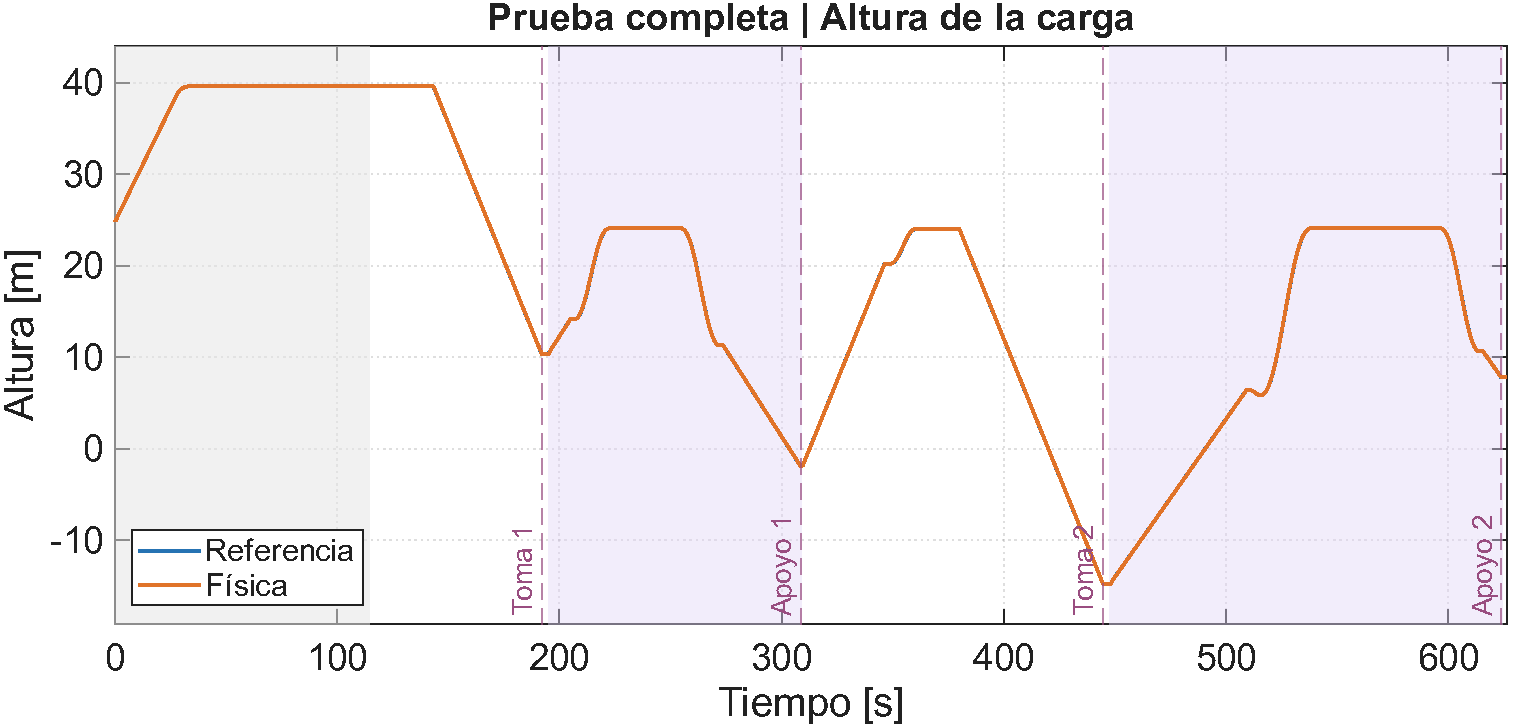
\includegraphics[width=0.98\textwidth]{resultados_prueba_ciclo_completo_en_simulink/y.pdf}
\caption{Altura física de la carga y referencia.}
\label{fig:prueba_ciclo_completo_en_simulink_y}
\end{figure}


\begin{figure}[!htbp]
\centering
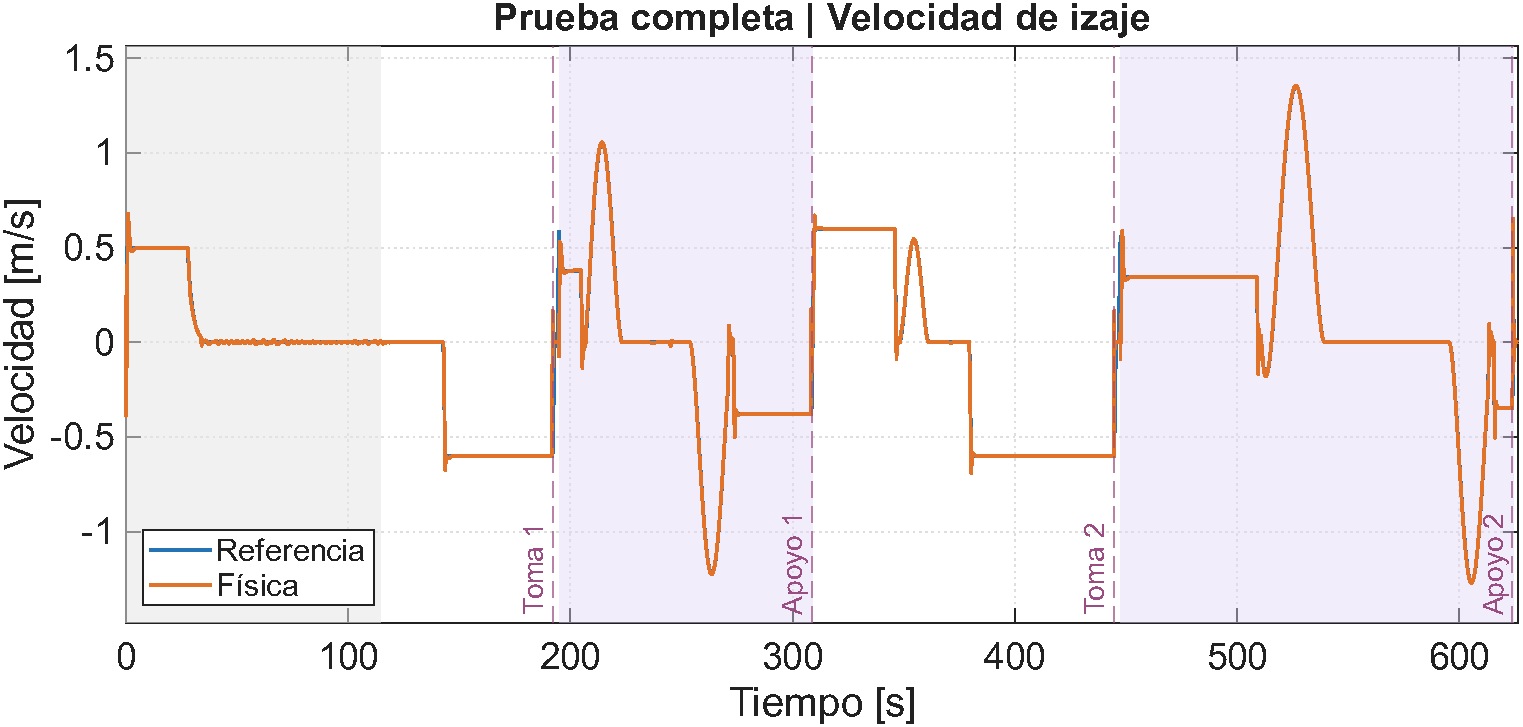
\includegraphics[width=0.98\textwidth]{resultados_prueba_ciclo_completo_en_simulink/vy.pdf}
\caption{Velocidad física de izaje y referencia.}
\label{fig:prueba_ciclo_completo_en_simulink_vy}
\end{figure}


\begin{figure}[!htbp]
\centering
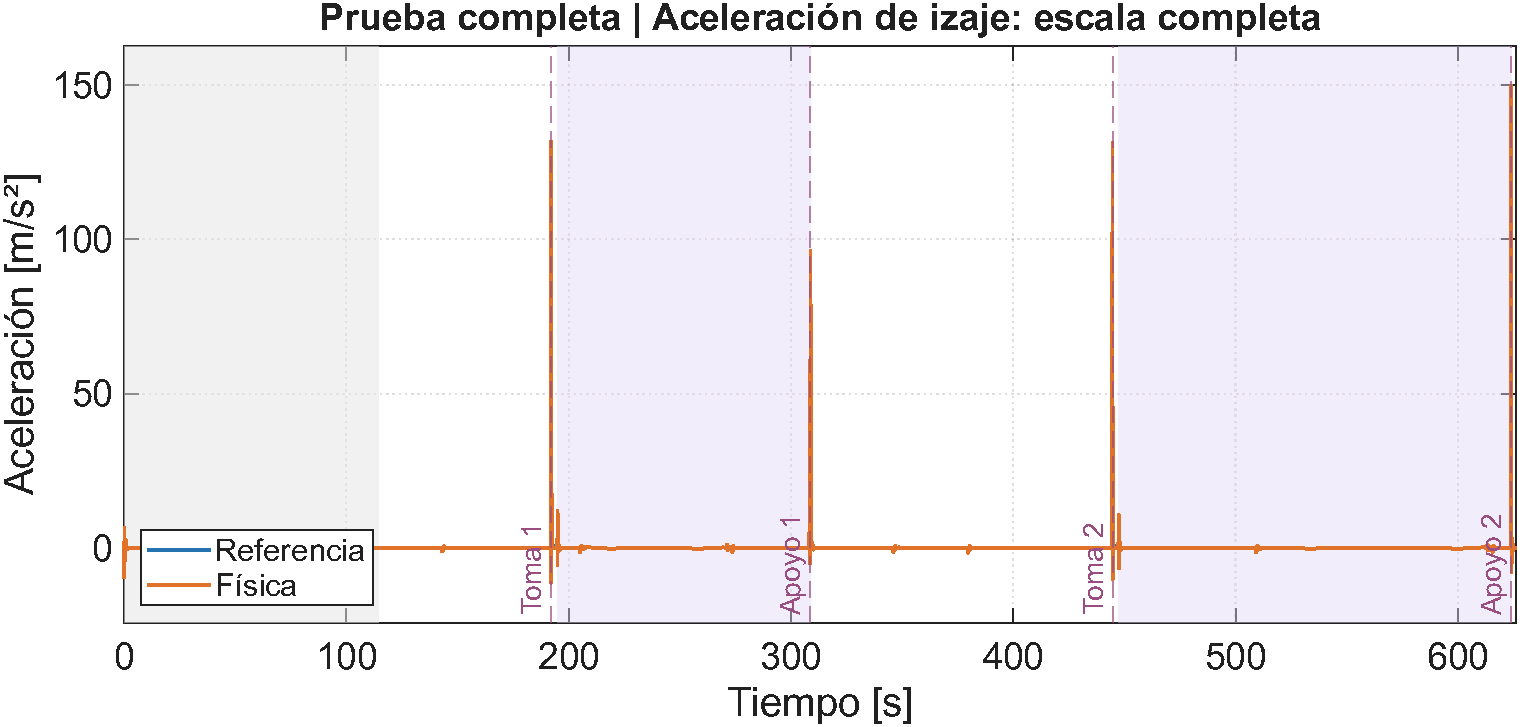
\includegraphics[width=0.98\textwidth]{resultados_prueba_ciclo_completo_en_simulink/ay.pdf}
\caption{Aceleración física de izaje y referencia, con escala completa.}
\label{fig:prueba_ciclo_completo_en_simulink_ay}
\end{figure}


\begin{figure}[!htbp]
\centering
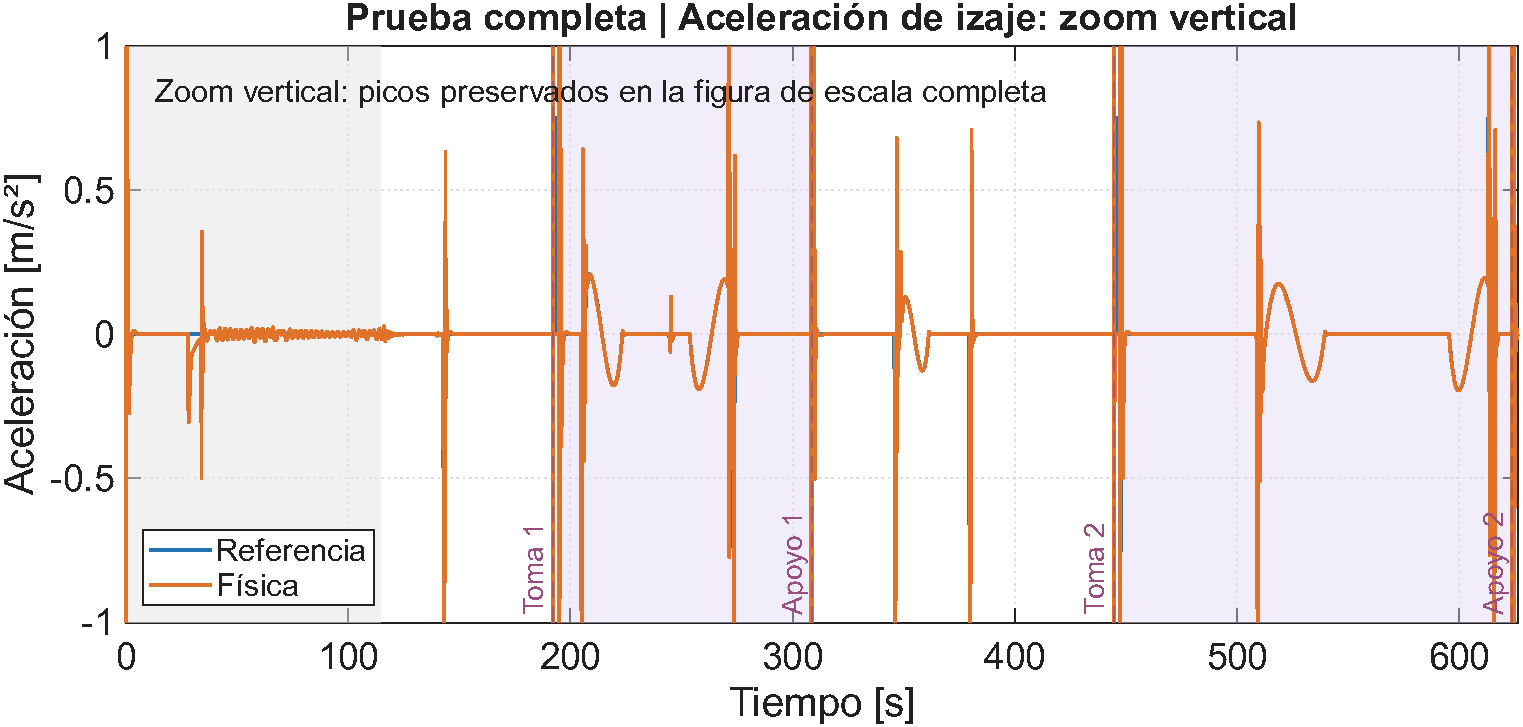
\includegraphics[width=0.98\textwidth]{resultados_prueba_ciclo_completo_en_simulink/ay_zoom.pdf}
\caption{Aceleración de izaje con zoom vertical; los extremos fuera del recuadro se conservan en la figura anterior.}
\label{fig:prueba_ciclo_completo_en_simulink_ay_zoom}
\end{figure}


\begin{figure}[!htbp]
\centering
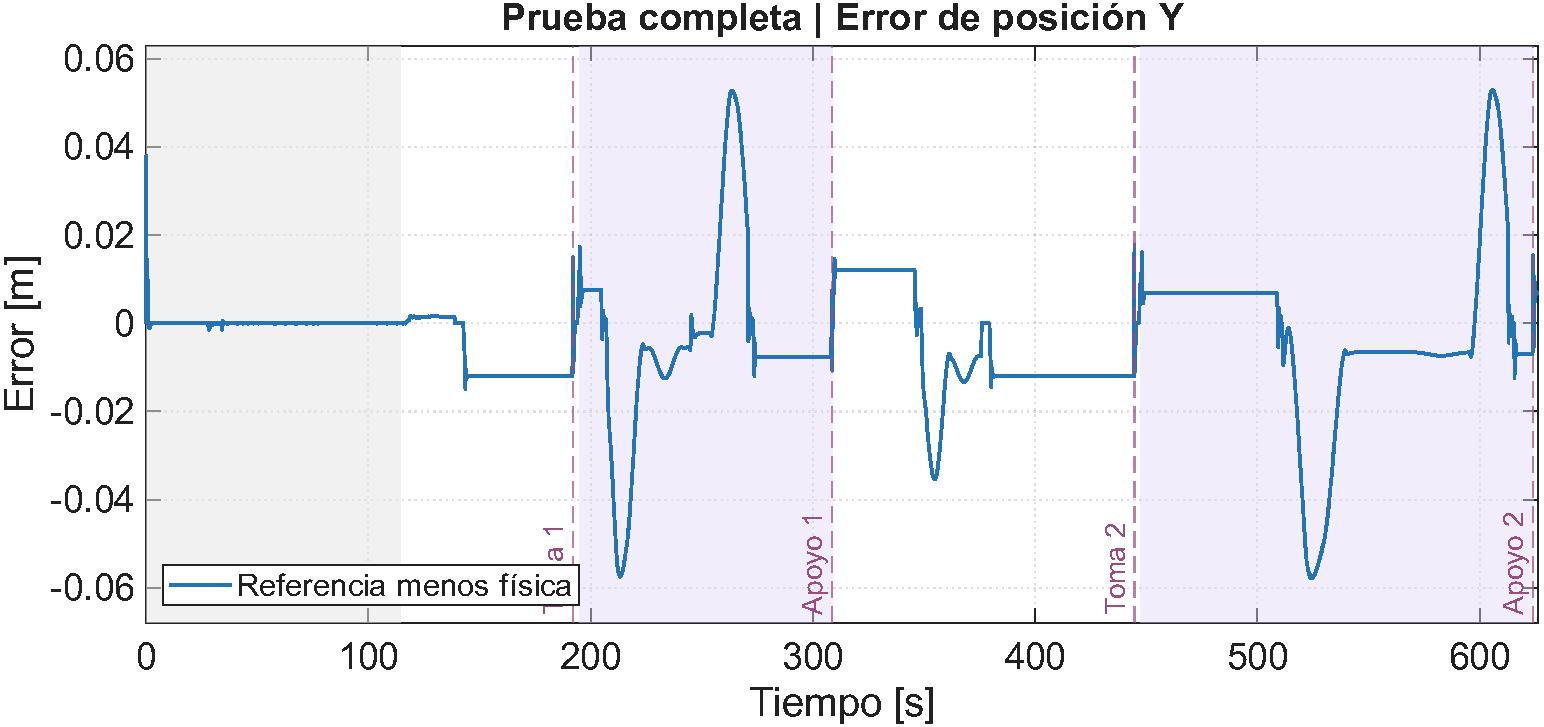
\includegraphics[width=0.98\textwidth]{resultados_prueba_ciclo_completo_en_simulink/error_y.pdf}
\caption{Error de altura, calculado como referencia menos altura física.}
\label{fig:prueba_ciclo_completo_en_simulink_error_y}
\end{figure}


\subsection{Balanceo y acción antisway}

El ángulo y la velocidad angular permiten evaluar el movimiento pendular durante las aproximaciones y los traslados. La velocidad angular física procede de la planta; la referencia de velocidad angular se obtiene posteriormente como derivada temporal de la referencia angular, por lo que se identifica como señal derivada. Las curvas de mando y las contribuciones de feedback y anticipación permiten relacionar el balanceo con la actuación del controlador.

En el traslado cargado 1, entre $206.88$ y $270.84~\mathrm{s}$, el máximo absoluto del ángulo físico fue de $0.0273~\mathrm{rad}$.

En el traslado cargado 2, entre $510.96$ y $612.88~\mathrm{s}$, el máximo absoluto del ángulo físico fue de $0.0094~\mathrm{rad}$.

Además del registro completo, se incluyen ampliaciones del intervalo posterior al relevamiento para observar el balanceo durante las aproximaciones y las transferencias sin que los transitorios del barrido determinen la escala.

\begin{figure}[!htbp]
\centering
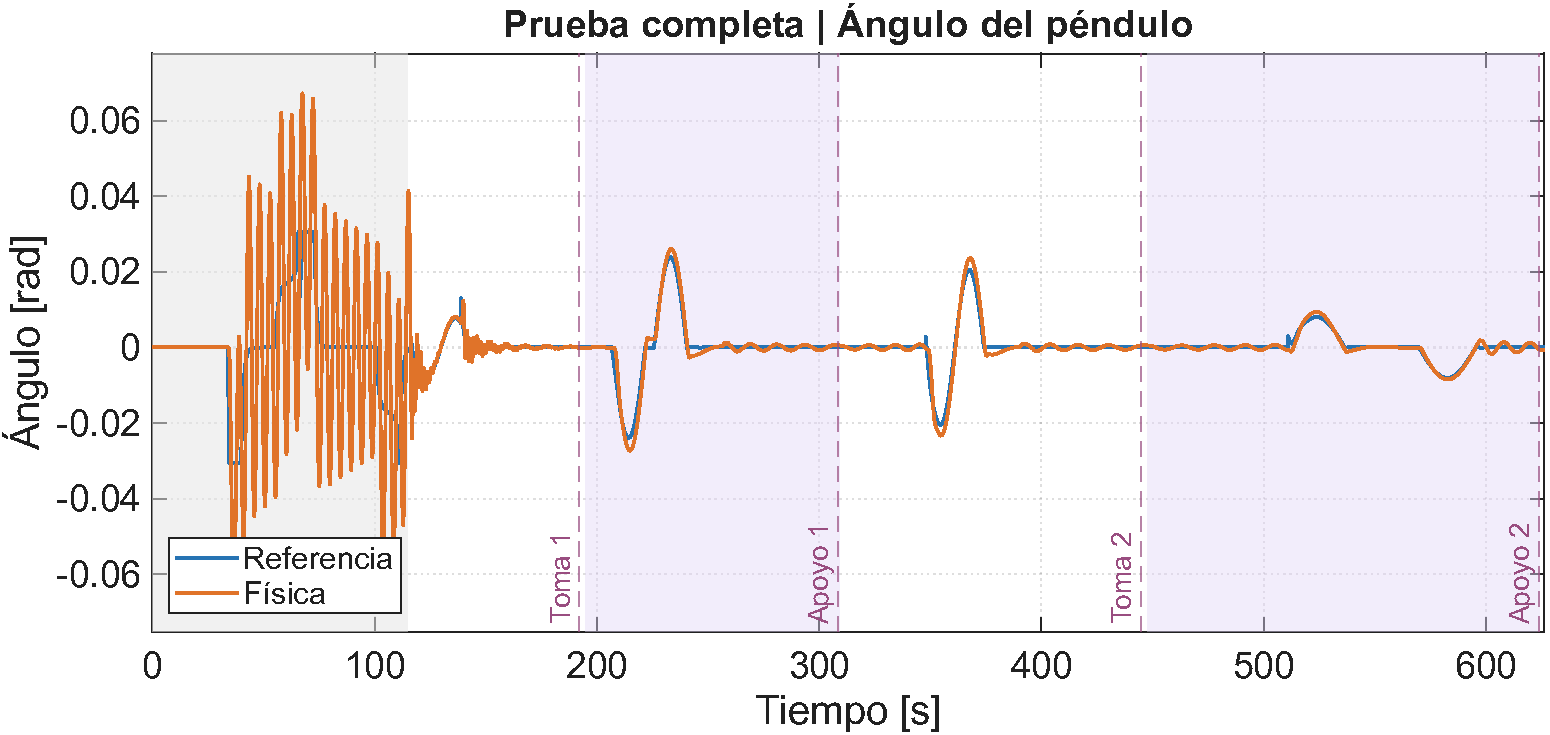
\includegraphics[width=0.98\textwidth]{resultados_prueba_ciclo_completo_en_simulink/theta.pdf}
\caption{Ángulo físico del péndulo y referencia angular: registro completo.}
\label{fig:prueba_ciclo_completo_en_simulink_theta}
\end{figure}


\begin{figure}[!htbp]
\centering
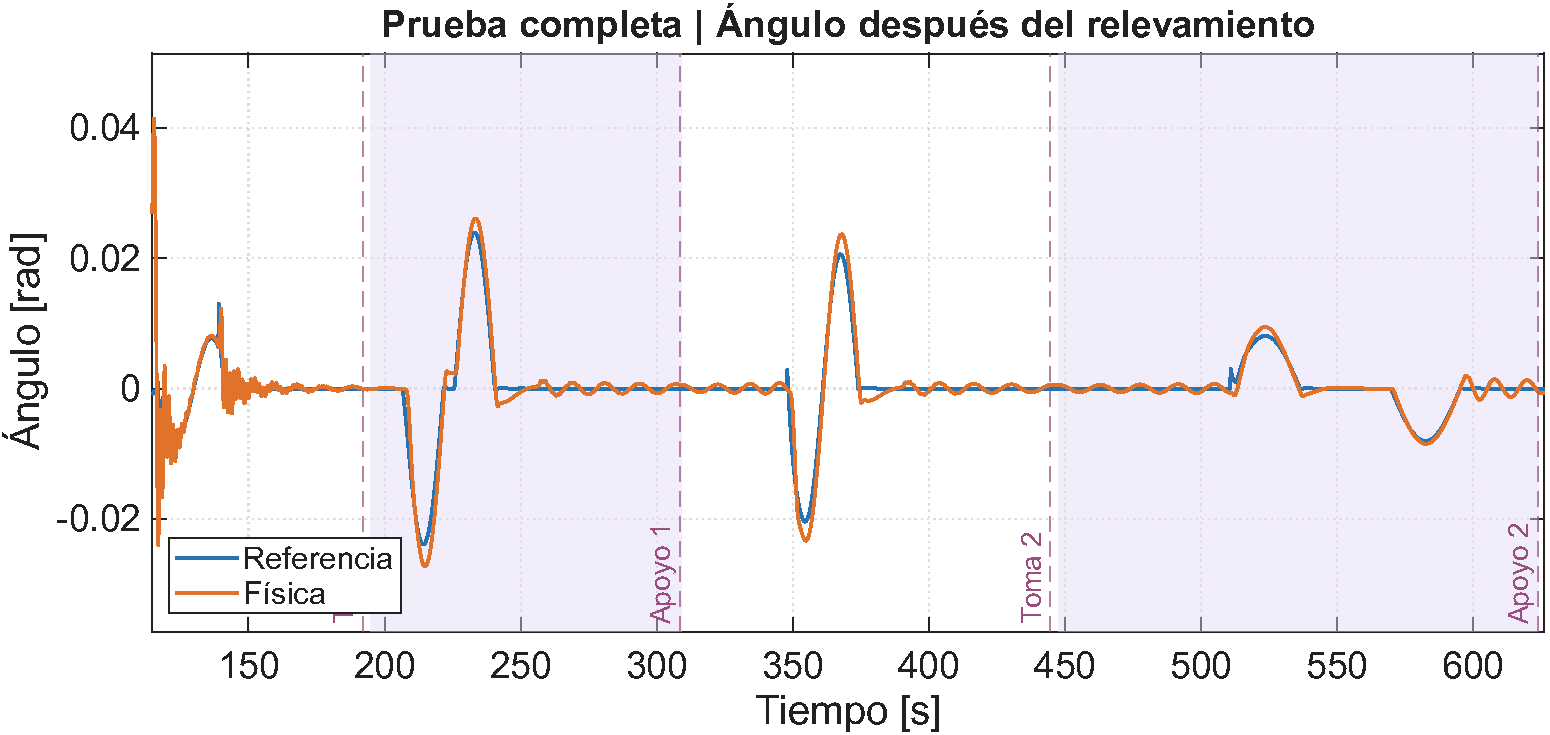
\includegraphics[width=0.98\textwidth]{resultados_prueba_ciclo_completo_en_simulink/theta_operativo.pdf}
\caption{Ángulo físico y referencia después del relevamiento, con escala ajustada a este intervalo.}
\label{fig:prueba_ciclo_completo_en_simulink_theta_operativo}
\end{figure}


\begin{figure}[!htbp]
\centering
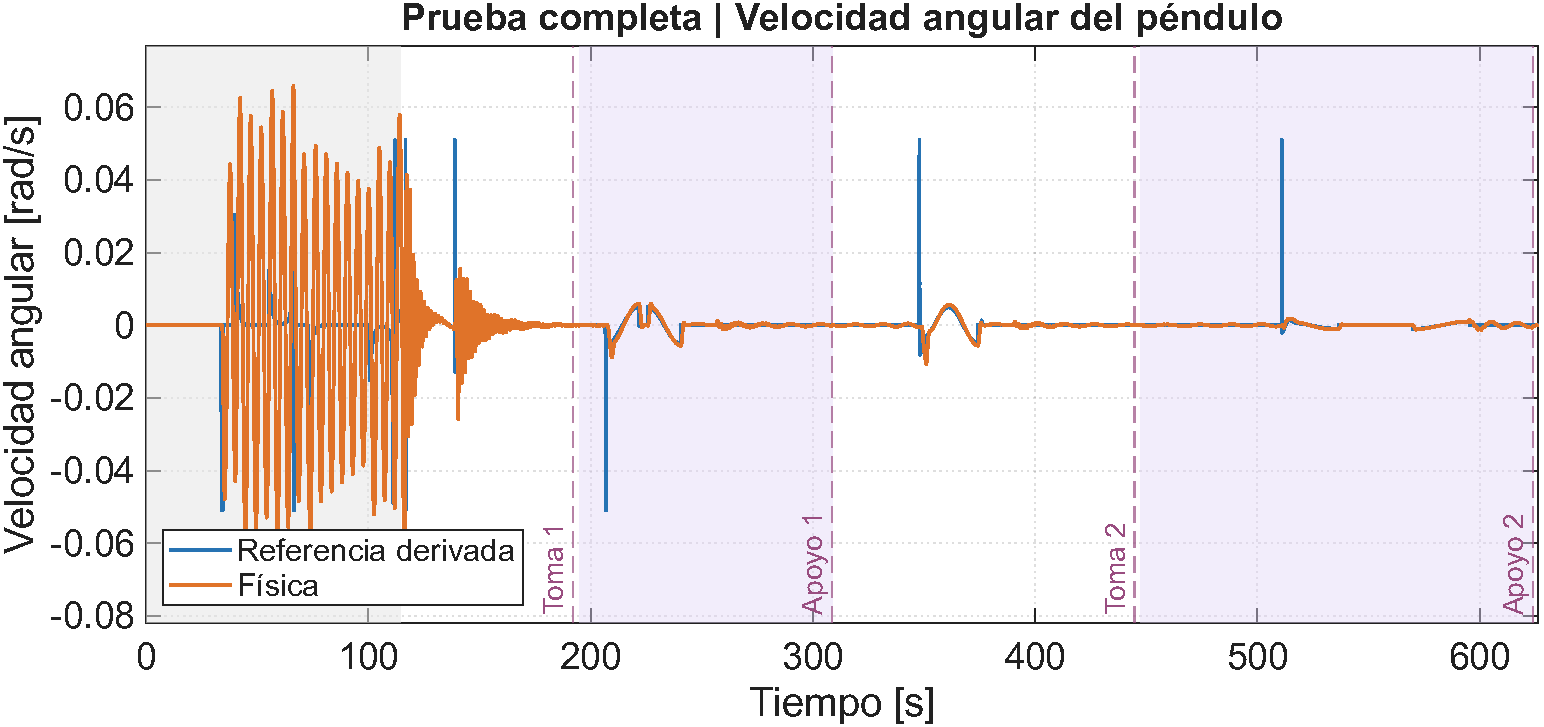
\includegraphics[width=0.98\textwidth]{resultados_prueba_ciclo_completo_en_simulink/omega.pdf}
\caption{Velocidad angular física y referencia derivada: registro completo.}
\label{fig:prueba_ciclo_completo_en_simulink_omega}
\end{figure}


\begin{figure}[!htbp]
\centering
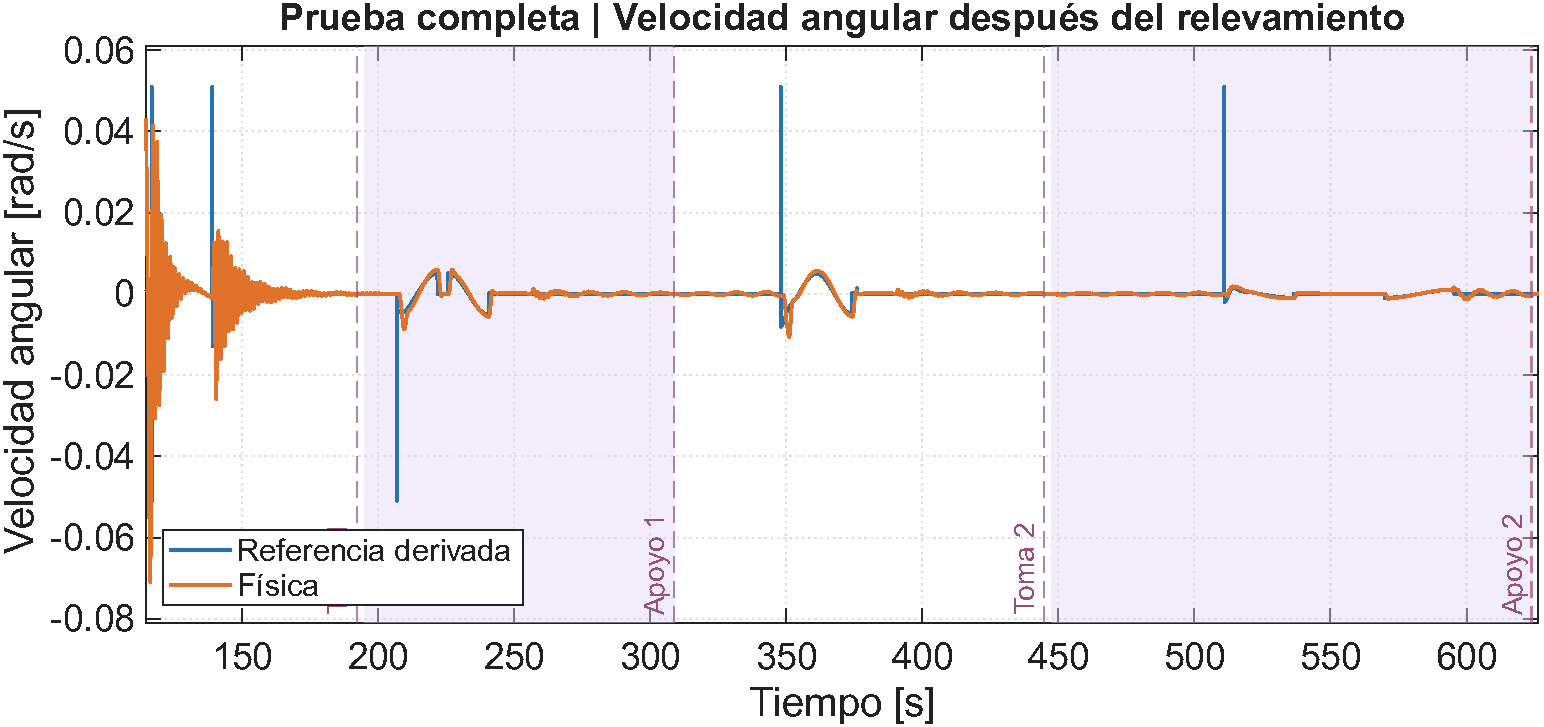
\includegraphics[width=0.98\textwidth]{resultados_prueba_ciclo_completo_en_simulink/omega_operativo.pdf}
\caption{Velocidad angular física y referencia derivada después del relevamiento.}
\label{fig:prueba_ciclo_completo_en_simulink_omega_operativo}
\end{figure}


\begin{figure}[!htbp]
\centering
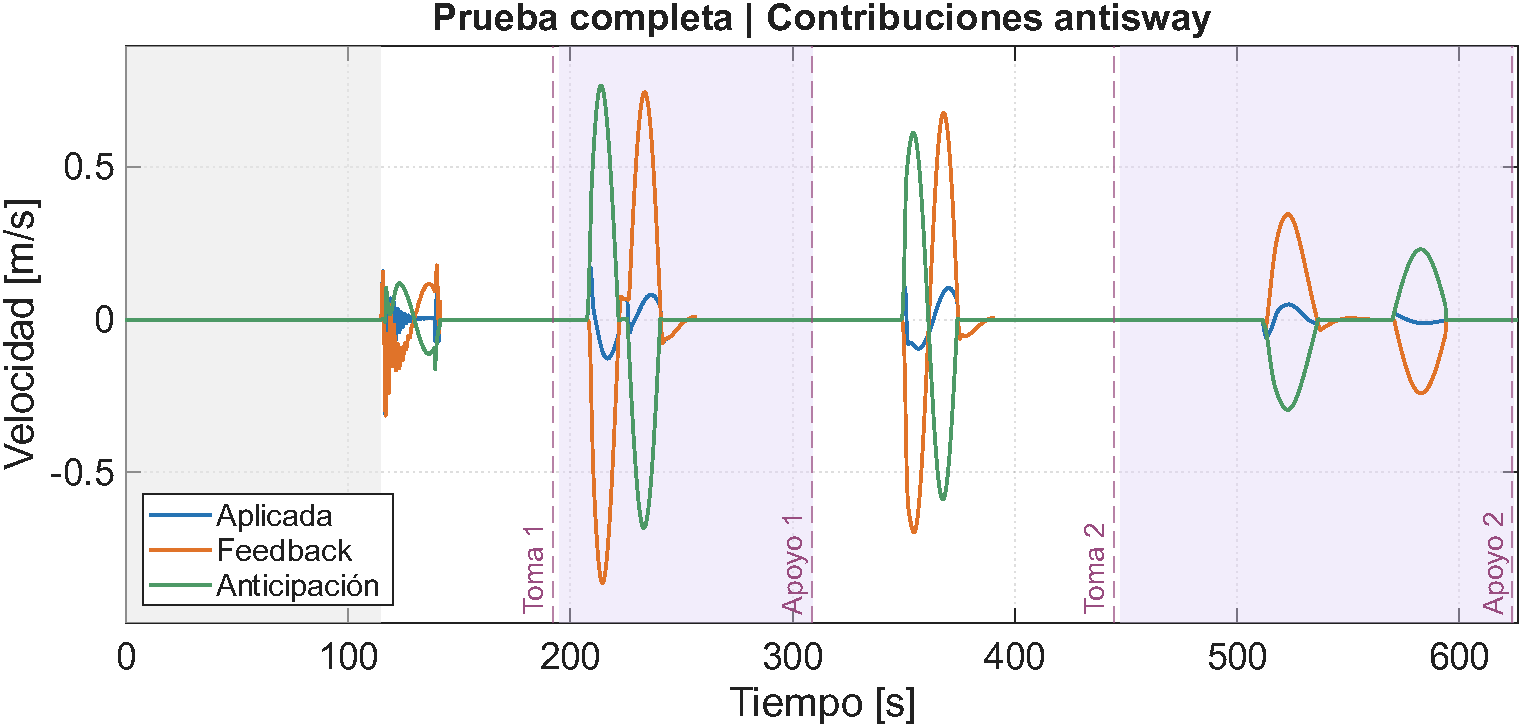
\includegraphics[width=0.98\textwidth]{resultados_prueba_ciclo_completo_en_simulink/antisway.pdf}
\caption{Contribución antisway aplicada y sus ramas de realimentación y anticipación.}
\label{fig:prueba_ciclo_completo_en_simulink_antisway}
\end{figure}


\begin{figure}[!htbp]
\centering
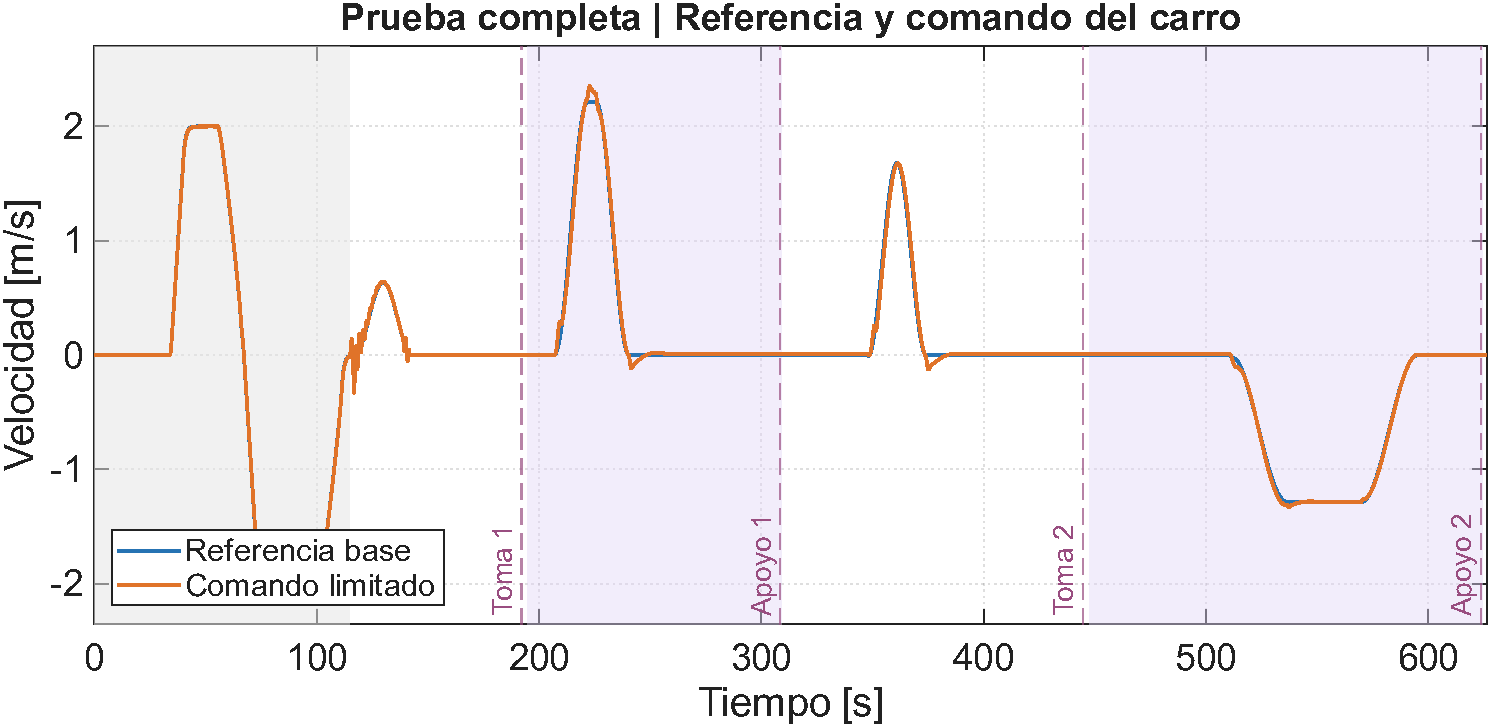
\includegraphics[width=0.98\textwidth]{resultados_prueba_ciclo_completo_en_simulink/comando.pdf}
\caption{Referencia de velocidad base y comando del controlador del carro.}
\label{fig:prueba_ciclo_completo_en_simulink_comando}
\end{figure}


\subsection{Torques, tensión y masa suspendida}

La comparación entre torque solicitado y torque físico permite observar las saturaciones y los transitorios del accionamiento. El torque del carro se muestra primero con el registro completo y luego desde la solicitud de arranque para observar el intervalo operativo sin que el valor de inicialización determine la escala. La tensión y la masa física complementan la evidencia de contacto, toma y liberación.

La masa física final fue de $15000.0~\mathrm{kg}$, correspondiente al conjunto vacío. El estado final y el balance del perfil corroboran las dos entregas.

\begin{figure}[!htbp]
\centering
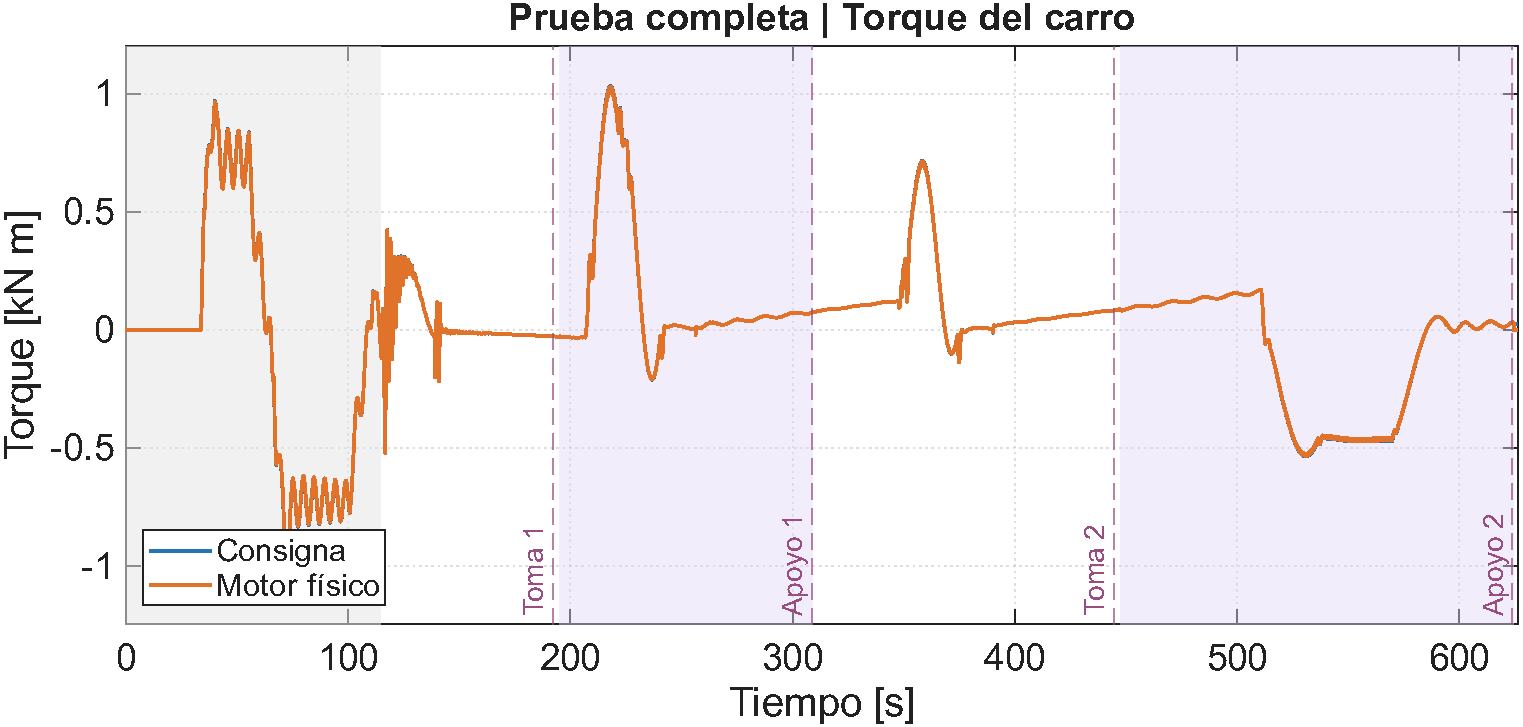
\includegraphics[width=0.98\textwidth]{resultados_prueba_ciclo_completo_en_simulink/tx.pdf}
\caption{Torque solicitado y torque físico del carro: registro completo.}
\label{fig:prueba_ciclo_completo_en_simulink_tx}
\end{figure}


\begin{figure}[!htbp]
\centering
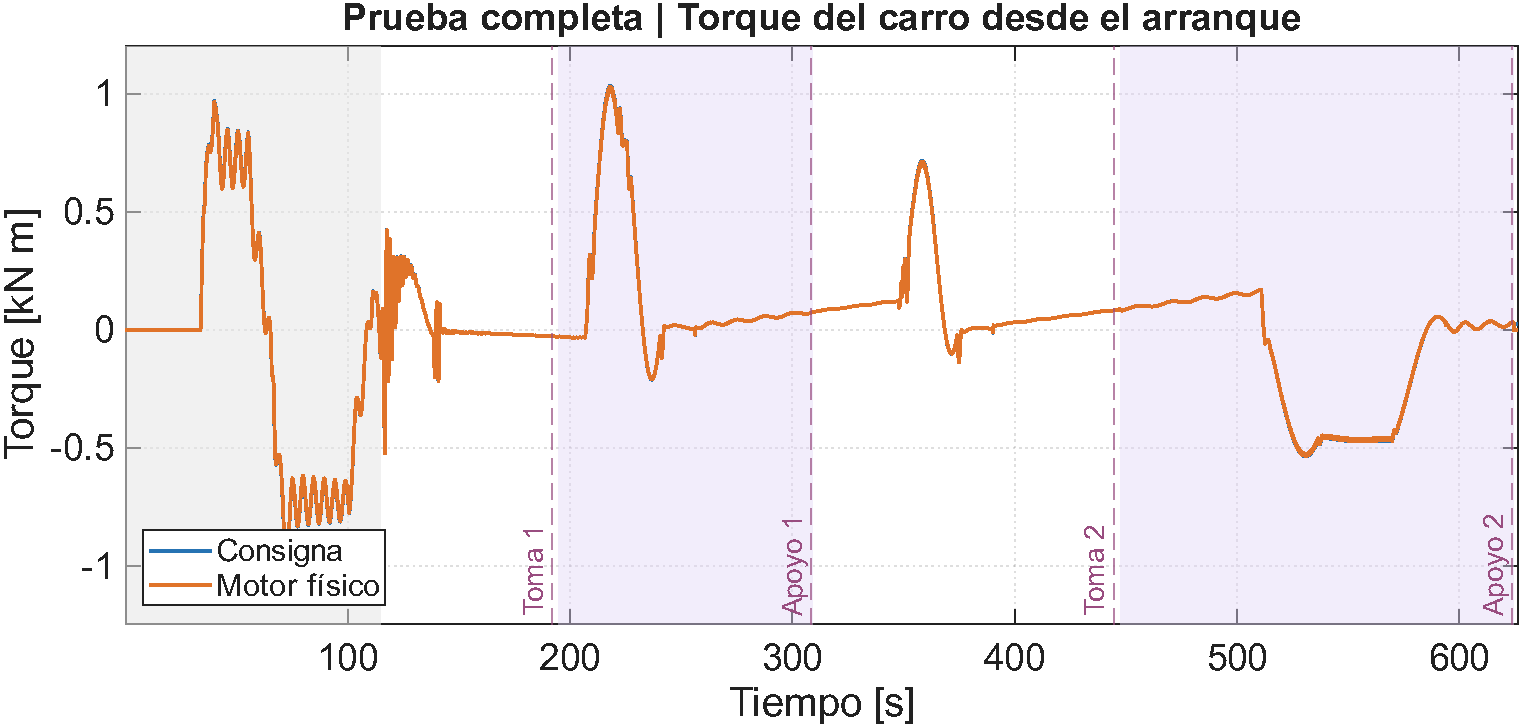
\includegraphics[width=0.98\textwidth]{resultados_prueba_ciclo_completo_en_simulink/tx_operativo.pdf}
\caption{Torque del carro desde el arranque: ampliación del intervalo operativo.}
\label{fig:prueba_ciclo_completo_en_simulink_tx_operativo}
\end{figure}


\begin{figure}[!htbp]
\centering
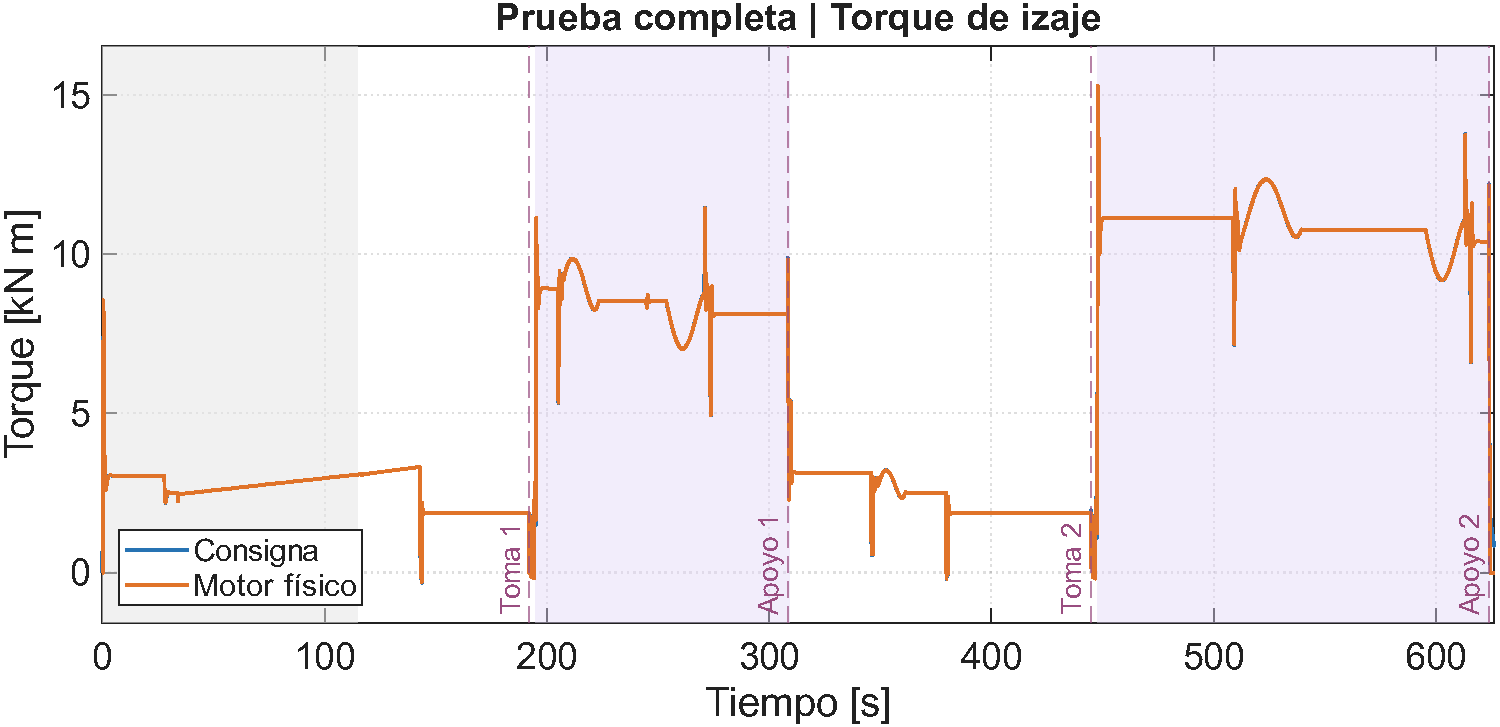
\includegraphics[width=0.98\textwidth]{resultados_prueba_ciclo_completo_en_simulink/ty.pdf}
\caption{Torque solicitado y torque físico del izaje.}
\label{fig:prueba_ciclo_completo_en_simulink_ty}
\end{figure}


\begin{figure}[!htbp]
\centering
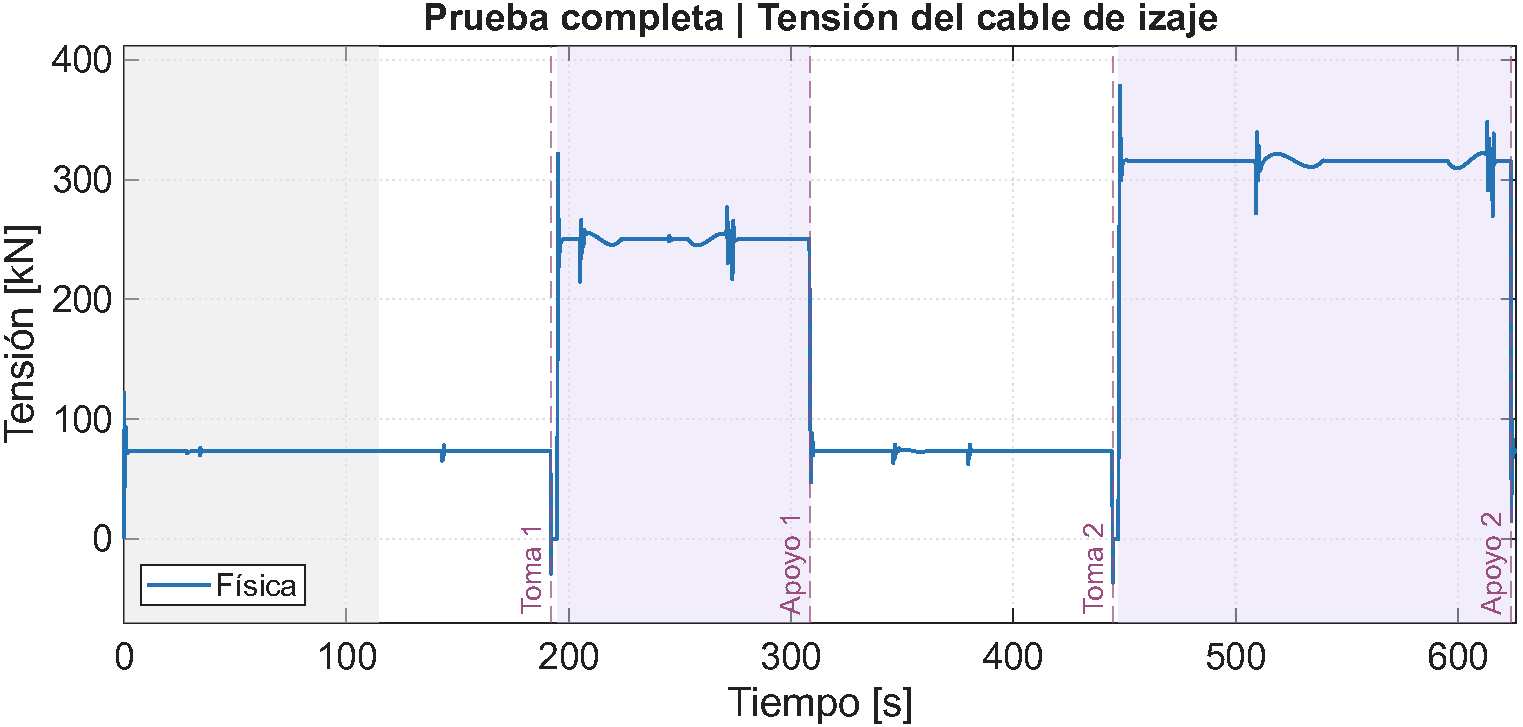
\includegraphics[width=0.98\textwidth]{resultados_prueba_ciclo_completo_en_simulink/tension.pdf}
\caption{Tensión física del cable durante relevamiento, tomas y entregas.}
\label{fig:prueba_ciclo_completo_en_simulink_tension}
\end{figure}


\begin{figure}[!htbp]
\centering
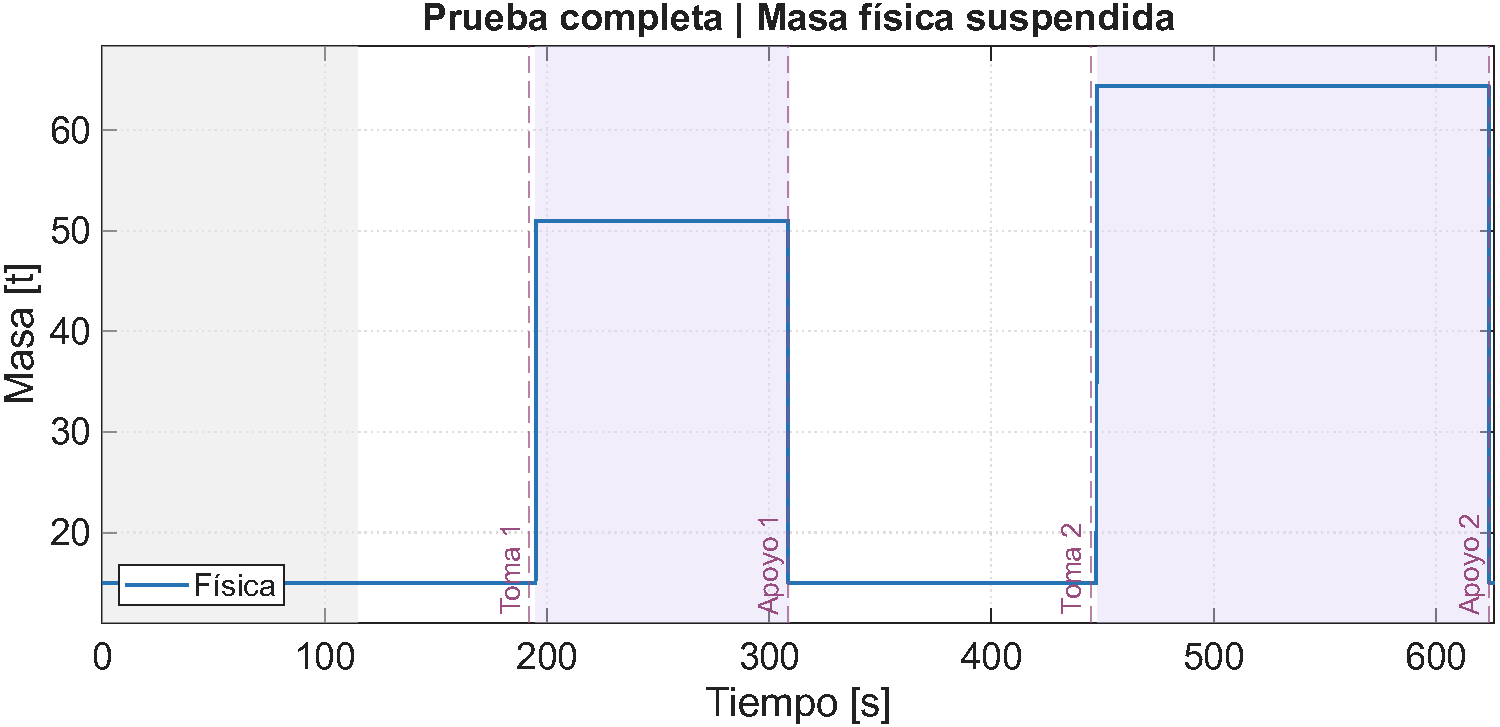
\includegraphics[width=0.98\textwidth]{resultados_prueba_ciclo_completo_en_simulink/masa.pdf}
\caption{Masa física suspendida durante las dos transferencias.}
\label{fig:prueba_ciclo_completo_en_simulink_masa}
\end{figure}


\subsection{Resultados y alcance de la prueba}

\begin{table}[!htbp]\centering

\caption{Comprobaciones de la Prueba ciclo completo en simulink.}\label{tab:criterios_prueba_ciclo_completo_en_simulink}

\begin{tabular}{L{10.8cm} C{2.6cm}}\toprule Criterio & Resultado\\\midrule

Barrido real terminado antes de la primera toma & Cumple\\

Dos tomas y dos entregas físicas en los destinos previstos & Cumple\\

Balance del perfil: dos bajas y dos altas de una altura de contenedor & Cumple\\

Conjunto vacío al finalizar la segunda entrega & Cumple\\

Ausencia de emergencia, falla de seguimiento y código de falla & Cumple\\

\bottomrule\end{tabular}\end{table}

La corrida produjo $395$ series registradas, incluyendo variables físicas, referencias, diagnósticos, perfil, mandos y seguridad. La integración del modelo no se alteró para reducir el registro: se conservó una de cada diez muestras de cada fuente, junto con sus tiempos originales. El operador y los mandos de la HMI se ejecutaron cada $40~\mathrm{ms}$; la actualización gráfica se realizó cada $200~\mathrm{ms}$. Se conservaron capturas de los eventos principales. Esta repetición se registró sin video.

Las bandas de las figuras distinguen el relevamiento y los intervalos entre toma y entrega; las marcas indican contactos físicos. No se representan modos de funcionamiento. El texto de colisión se omitió del alarmero para la presentación, conservando su señal y las protecciones del modelo. Esta prueba nominal no inyecta fallas y no sustituye ensayos específicos de seguridad.

\begin{figure}[!htbp]
\centering
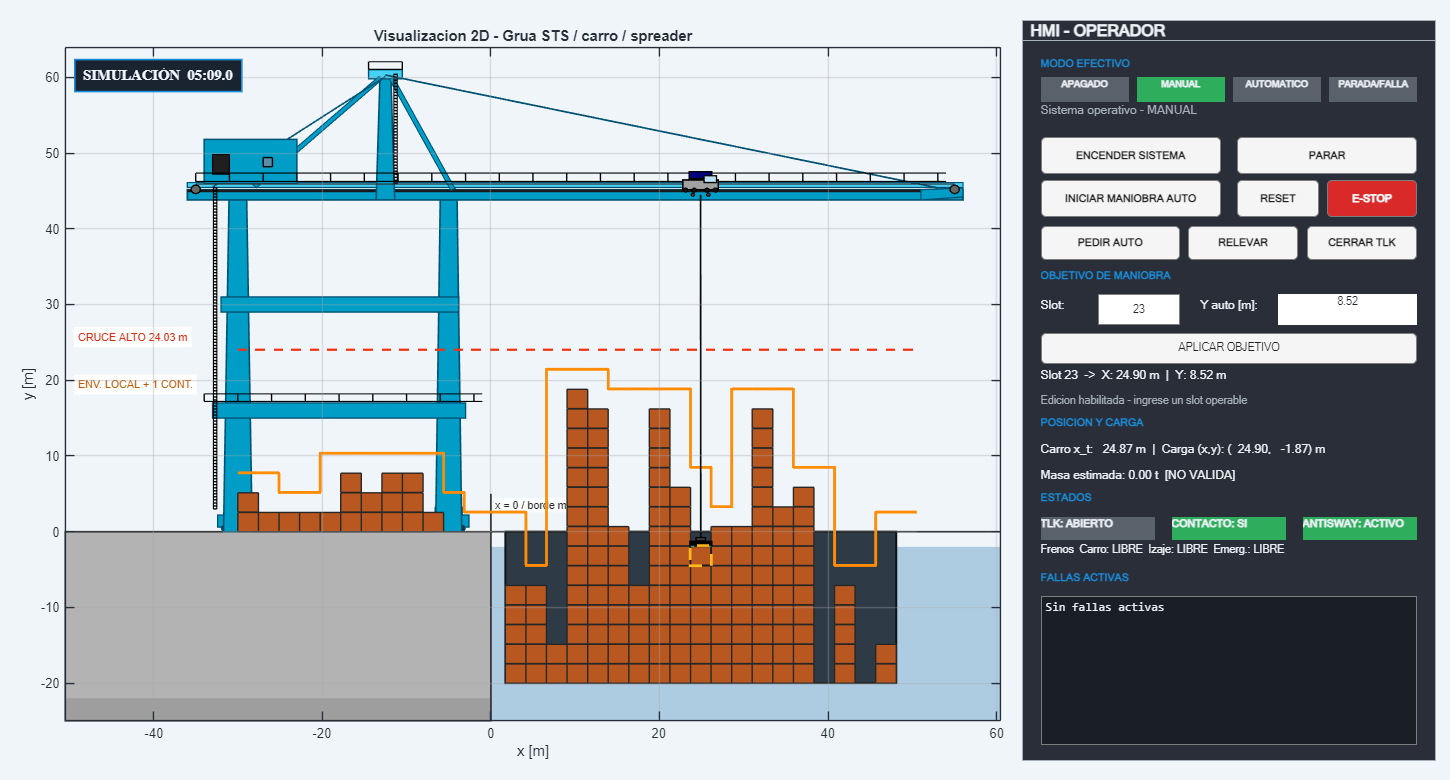
\includegraphics[width=0.98\textwidth]{resultados_prueba_ciclo_completo_en_simulink/transferencia_2.png}
\caption{Primera entrega física en la posición central del barco.}
\label{fig:prueba_ciclo_completo_en_simulink_transferencia_2}
\end{figure}


\begin{figure}[!htbp]
\centering
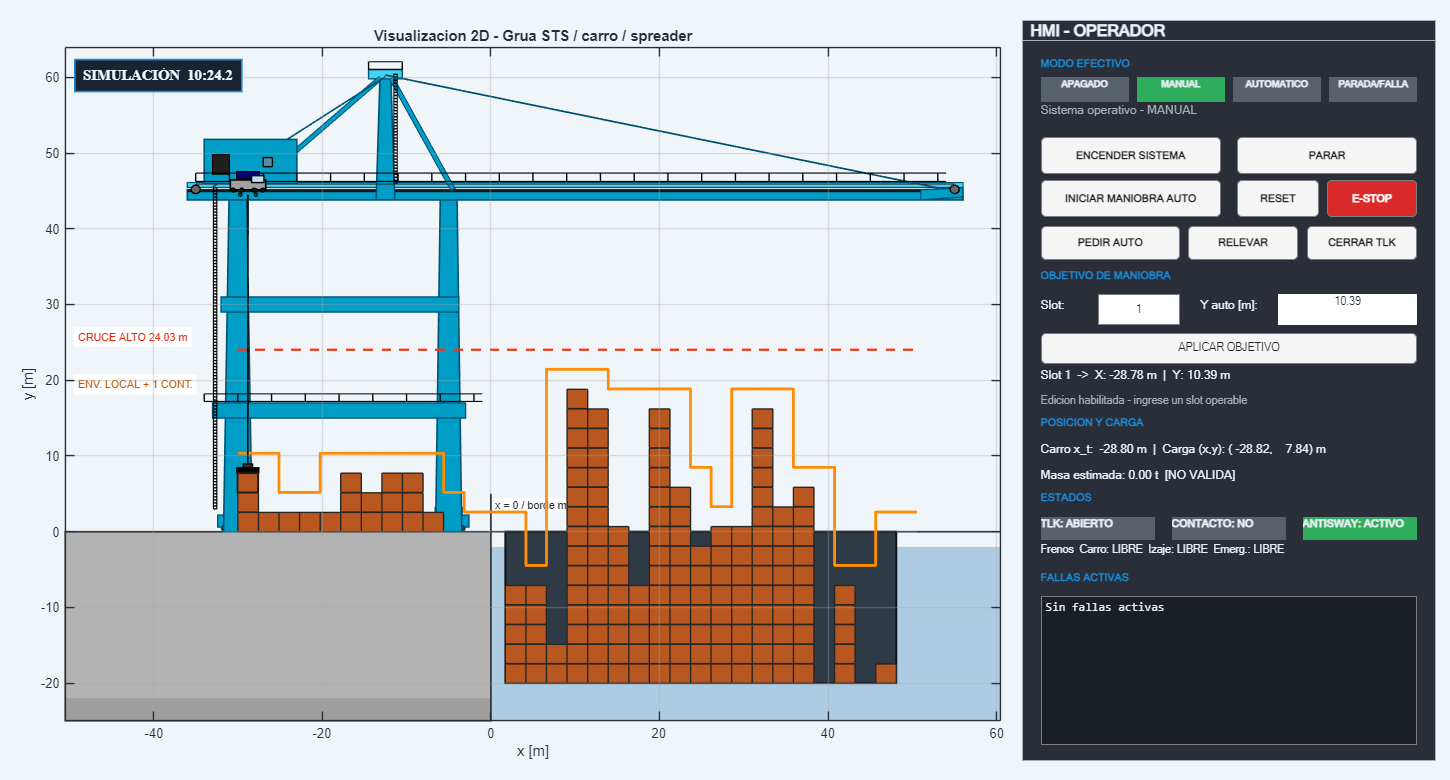
\includegraphics[width=0.98\textwidth]{resultados_prueba_ciclo_completo_en_simulink/transferencia_4.png}
\caption{Segunda entrega física en el extremo izquierdo del muelle.}
\label{fig:prueba_ciclo_completo_en_simulink_transferencia_4}
\end{figure}


\begin{figure}[!htbp]
\centering
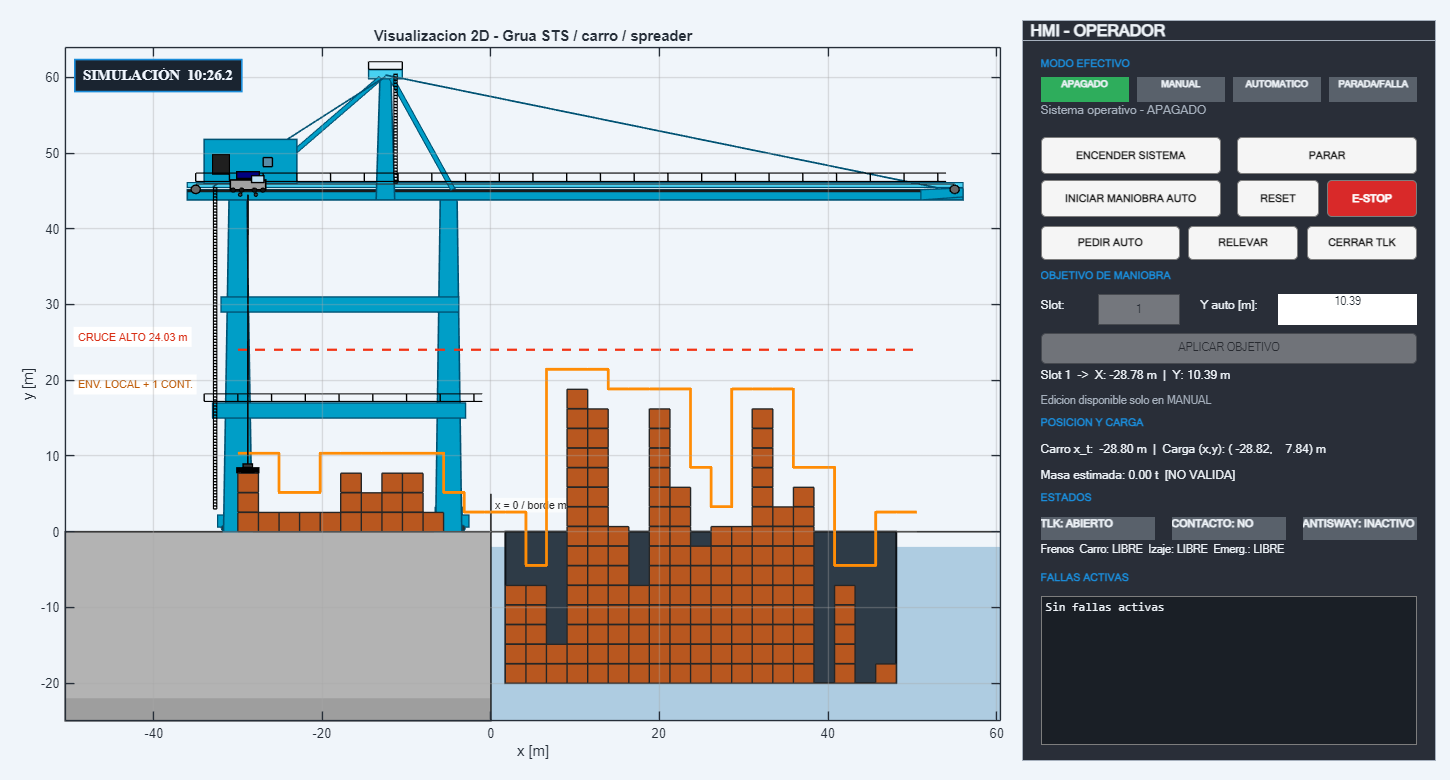
\includegraphics[width=0.98\textwidth]{resultados_prueba_ciclo_completo_en_simulink/05_final.png}
\caption{Estado final de la visualización y HMI después de las dos transferencias y la parada normal.}
\label{fig:prueba_ciclo_completo_en_simulink_05_final}
\end{figure}


Incluyendo el relevamiento, la duración equivale a aproximadamente $11.5$ contenedores por hora para esta secuencia de dos entregas. Es un cociente orientativo de una sola corrida; no demuestra por sí solo una productividad sostenida ni reemplaza una evaluación de ciclos repetidos.



\clearpage

\subsection{Pruebas del nivel de seguridad}
Además de la maniobra nominal deben ensayarse fallas inyectadas:
\begin{itemize}
    \item activación de cada límite último;
    \item exceso de velocidad de izaje;
    \item pulsador de emergencia;
    \item congelamiento del pulso de \textit{watchdog};
    \item pérdida del permiso global durante automático;
    \item intento de reinicio con la causa todavía activa.
\end{itemize}
En cada caso se comprueba que los permisos y frenos coincidan con la matriz causa--efecto y que la recuperación exija un reinicio explícito.

% IMAGEN A INSERTAR: registros de una prueba de emergencia total.
\figplaceholder{Gráficas de causa, estado de seguridad, permisos y comandos de freno durante una emergencia.}{Respuesta temporal ante una condición de seguridad.}

% Secciones agregadas: pruebas CODESYS manual y ST, 2026-10-05.
% Ensayos actualizados: cuatro corridas del banco de medio ciclo.
\clearpage
\section{Pruebas de medio ciclo con CODESYS manual}
\label{sec:ensayo_codesys_manual}
\subsection{Objetivo y condiciones comunes}
Se compararon los autómatas supervisor y de seguridad programados manualmente en CODESYS mediante SFC y los autómatas en texto estructurado obtenidos mediante generación automática de código para PLC de Simulink. La planta, sensores, reguladores, visualización y HMI permanecieron en Simulink, conectados al PLC por OPC UA. Los términos manual y automático identifican la implementación de los autómatas; ambas maniobras combinan conducción manual y traslado automático.

Las cuatro pruebas comparten perfil físico, masas, ganancias, condiciones iniciales y operador. Antes de cada corrida se realizó Reset en caliente y se puso el PLC en RUN. Se precargaron las 33 alturas reales de la escena, con perfil válido y barrido no completado. El ensayo comienza directamente con la toma en el muelle y termina al entregar o al detenerse por el criterio establecido; no incluye barrido LiDAR, retorno vacío ni segunda toma.

\begin{table}[!htbp]\centering\small
\caption{Condiciones comunes del banco actualizado.}\label{tab:condiciones_medio_codesys}
\begin{tabular}{L{.31\textwidth}L{.61\textwidth}}\toprule
Condición & Configuración\\\midrule
Inicio y destino & $x=-26.34~\mathrm{m}$, altura $25~\mathrm{m}$, reposo; retiro del slot 2 y destino slot 22, centro $22.46~\mathrm{m}$.\\
Masa suspendida & Spreader: $15\,000~\mathrm{kg}$; contenedor: $36\,863~\mathrm{kg}$; conjunto cargado: $51\,863~\mathrm{kg}$.\\
Perfil & 33 alturas físicas; máximo inicial $18.85~\mathrm{m}$; contenedor de altura $2.59~\mathrm{m}$.\\
Control & Reguladores de carro e izaje comunes; observadores discretizados por Tustin; rampa de habilitación antisway de $2~\mathrm{s}$ y límite de variación de su término anticipativo de $0.25~\mathrm{m/s^2}$.\\
Variante & Ganancia cero o uno sobre la contribución antisway antes de sumarla al comando; cálculo interno conservado.\\
Tiempos & Control: $1~\mathrm{ms}$; actualización de autómatas por trama simulada de $20~\mathrm{ms}$; operador y rejilla de análisis: $40~\mathrm{ms}$.\\
Vigilancia & Latido de enlace independiente en tiempo real; timeout de comunicación de $3~\mathrm{s}$. La sincronización de las máquinas de estados usa el tiempo simulado.\\
Finalización & Sin antisway: límite solicitado de $180~\mathrm{s}$. Con antisway: continuar sin fallas hasta entrega o hasta diagnóstico de bloqueo.\\\bottomrule
\end{tabular}\end{table}

La adaptación del banco separa el reloj de la maniobra simulada de la vigilancia real de comunicaciones. Permite reproducir la secuencia aunque la visualización y el registro ralenticen Simulink. No constituye una validación de ejecución en tiempo real sobre una máquina física. Los límites, ganancias y criterios de descarga no se relajaron para obtener entregas.

\subsection{Procedimiento y comprobación de entrega}
El operador solicita START, entra a manual, aproxima y desciende hasta contacto en el origen, cierra twistlocks, confirma toma y selecciona destino. Eleva manualmente hasta la altura local segura más $1~\mathrm{m}$ y solicita automático después de esperar al menos $2~\mathrm{s}$ y alcanzar $|v_y|<0.03~\mathrm{m/s}$. Cerca del barco solicita manual sólo si el error horizontal es menor que $0.5~\mathrm{m}$, $|v_x|<0.25~\mathrm{m/s}$ y la altura no supera la consigna automática más $0.25~\mathrm{m}$. Después desciende hasta apoyo, abre twistlocks y comprueba la descarga física antes de STOP.

La compuerta de descenso automático exige simultáneamente error horizontal no mayor que $0.08~\mathrm{m}$, velocidad horizontal no mayor que $0.06~\mathrm{m/s}$, $|\theta|\leq0.005~\mathrm{rad}$ y $|\omega|\leq0.012~\mathrm{rad/s}$. Llegar horizontalmente no equivale a completar el descenso. La entrega se confirma por la masa física final de $15\,000~\mathrm{kg}$ y el incremento de $2.59~\mathrm{m}$ en el perfil del destino, además del retiro en el origen. Una indicación de carga vacía del PLC, por sí sola, no confirma la transferencia física.

\subsection{CODESYS manual sin antisway: traslado y espera sin entrega}
START se solicitó a $3.24~\mathrm{s}$, el modo manual se observó a $3.76~\mathrm{s}$ y el cierre de twistlocks se solicitó a $46.64~\mathrm{s}$. La masa cargada se confirmó a $49.52~\mathrm{s}$ y el despegue físico a $50.00~\mathrm{s}$. El operador solicitó automático a $75.32~\mathrm{s}$ y lo observó a $75.44~\mathrm{s}$; la llegada horizontal se registró a $105.68~\mathrm{s}$. No hubo transferencia a manual en destino ni entrega.

La prueba se detuvo a $187.20~\mathrm{s}$ con el contenedor retenido. El límite de tres minutos fue solicitado cuando la simulación ya había superado ese instante; por ello se conserva el tiempo real de parada de la corrida y no se recorta a $180~\mathrm{s}$. Es una prueba válida de comportamiento sin antisway, con medio ciclo incompleto.

Las posiciones muestran la toma, elevación y cruce hacia el barco, seguido de permanencia en altura. Las velocidades disminuyen cerca del destino, mientras las aceleraciones conservan los transitorios de contacto y cambio de movimiento. Las referencias y señales del controlador tienen cobertura hasta $130.72~\mathrm{s}$; muchas señales físicas hasta $177.305~\mathrm{s}$. La telemetría del operador conserva posiciones y modo hasta $187.20~\mathrm{s}$. Las curvas nativas se interrumpen al finalizar su registro: los espacios restantes no representan valores nulos ni reposo demostrado.

\begin{figure}[!htbp]
\centering
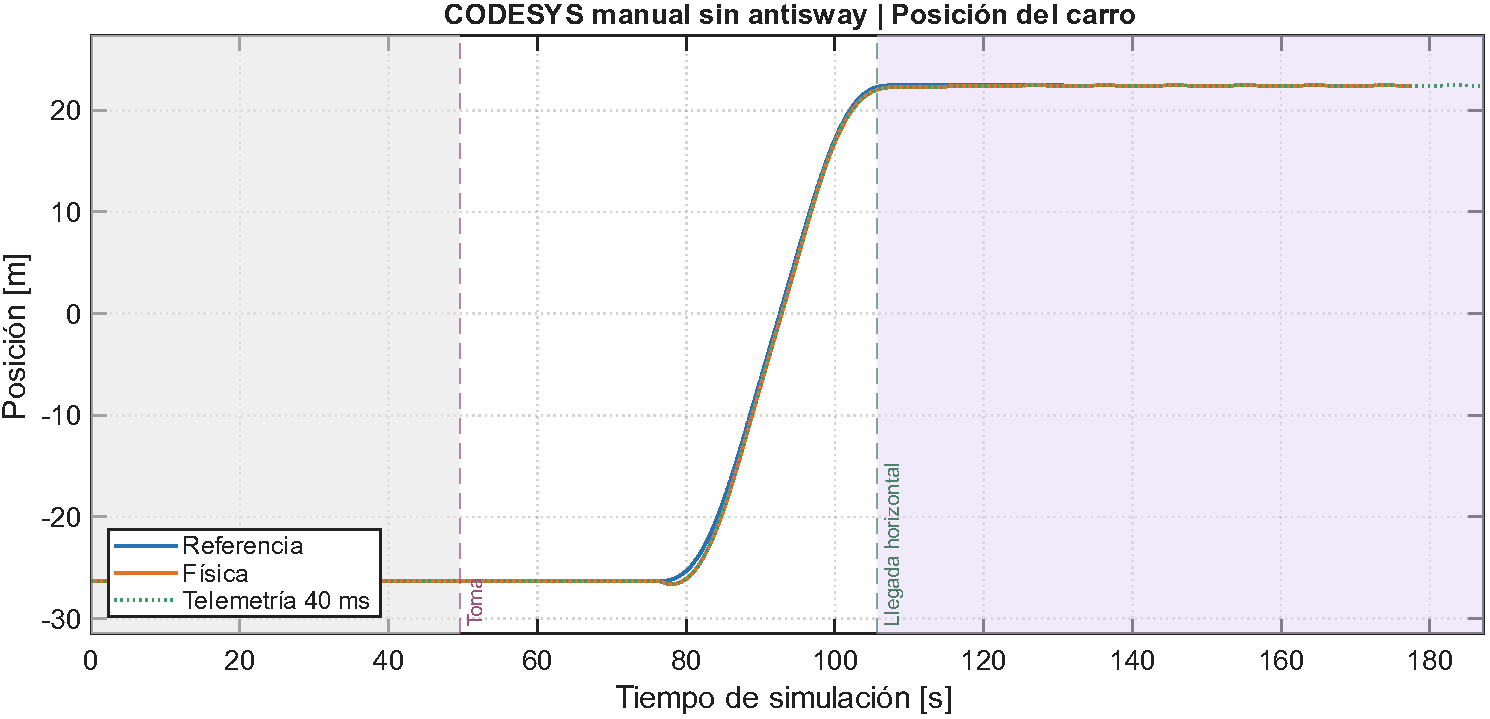
\includegraphics[width=0.98\textwidth]{graficas_individuales/manual_sin_x.pdf}
\caption{CODESYS manual sin antisway: Posición del carro: referencia y evolución física. La telemetría prolonga las posiciones hasta la parada; las referencias terminan en su última muestra.}\label{fig:individual_manual_sin_x}
\end{figure}

\begin{figure}[!htbp]
\centering
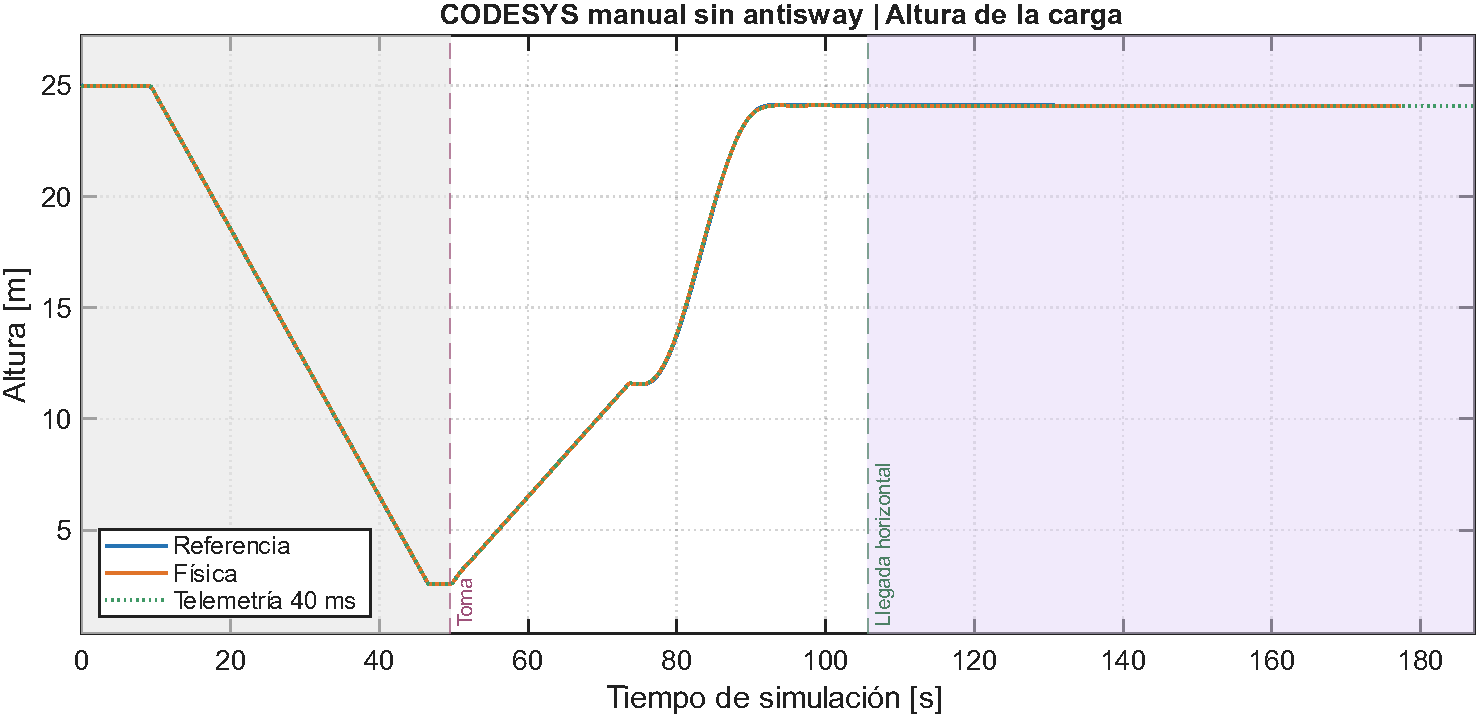
\includegraphics[width=0.98\textwidth]{graficas_individuales/manual_sin_y.pdf}
\caption{CODESYS manual sin antisway: Altura de la carga: referencia y evolución física. La telemetría prolonga las posiciones hasta la parada; las referencias terminan en su última muestra.}\label{fig:individual_manual_sin_y}
\end{figure}

\begin{figure}[!htbp]
\centering
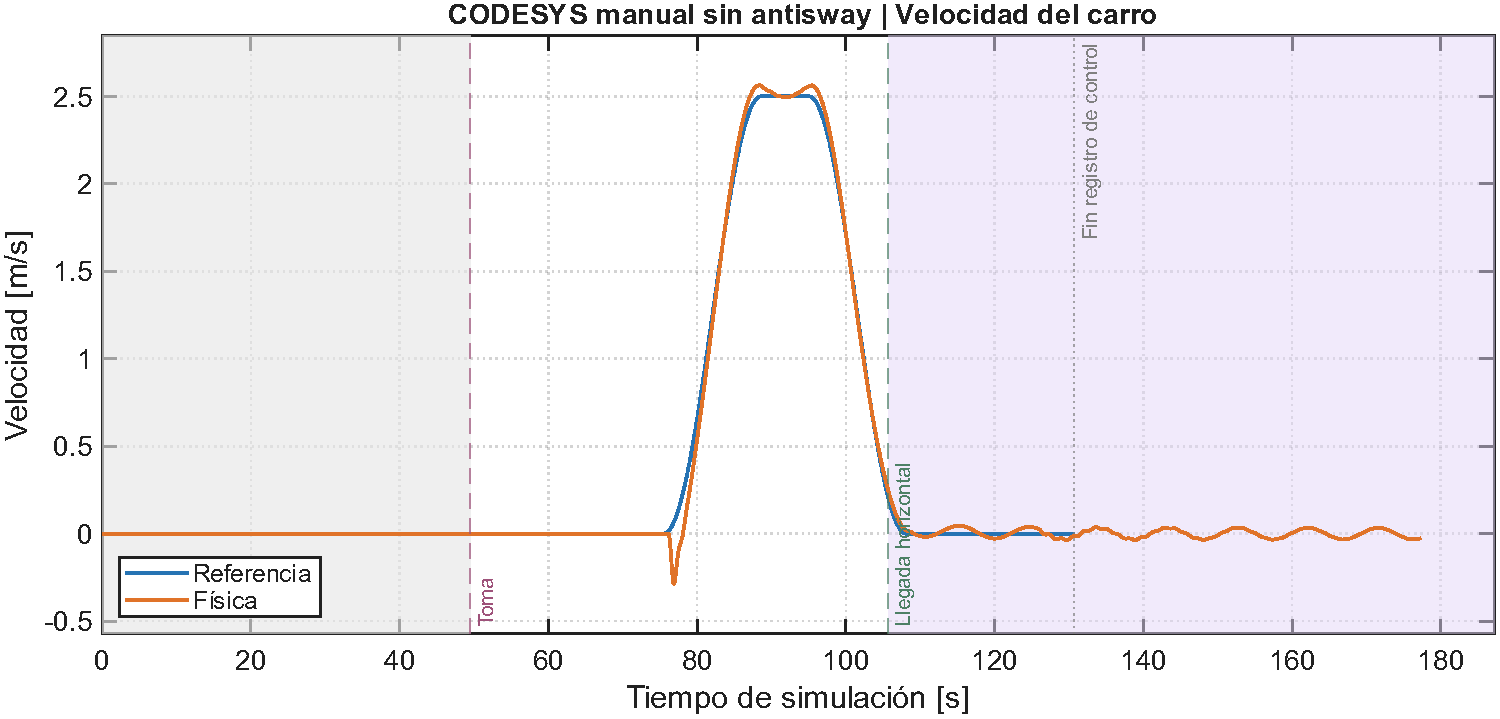
\includegraphics[width=0.98\textwidth]{graficas_individuales/manual_sin_vx.pdf}
\caption{CODESYS manual sin antisway: Velocidad del carro: referencia y señal física. Se respeta la cobertura parcial de las señales y no se extrapolan datos faltantes.}\label{fig:individual_manual_sin_vx}
\end{figure}

\begin{figure}[!htbp]
\centering
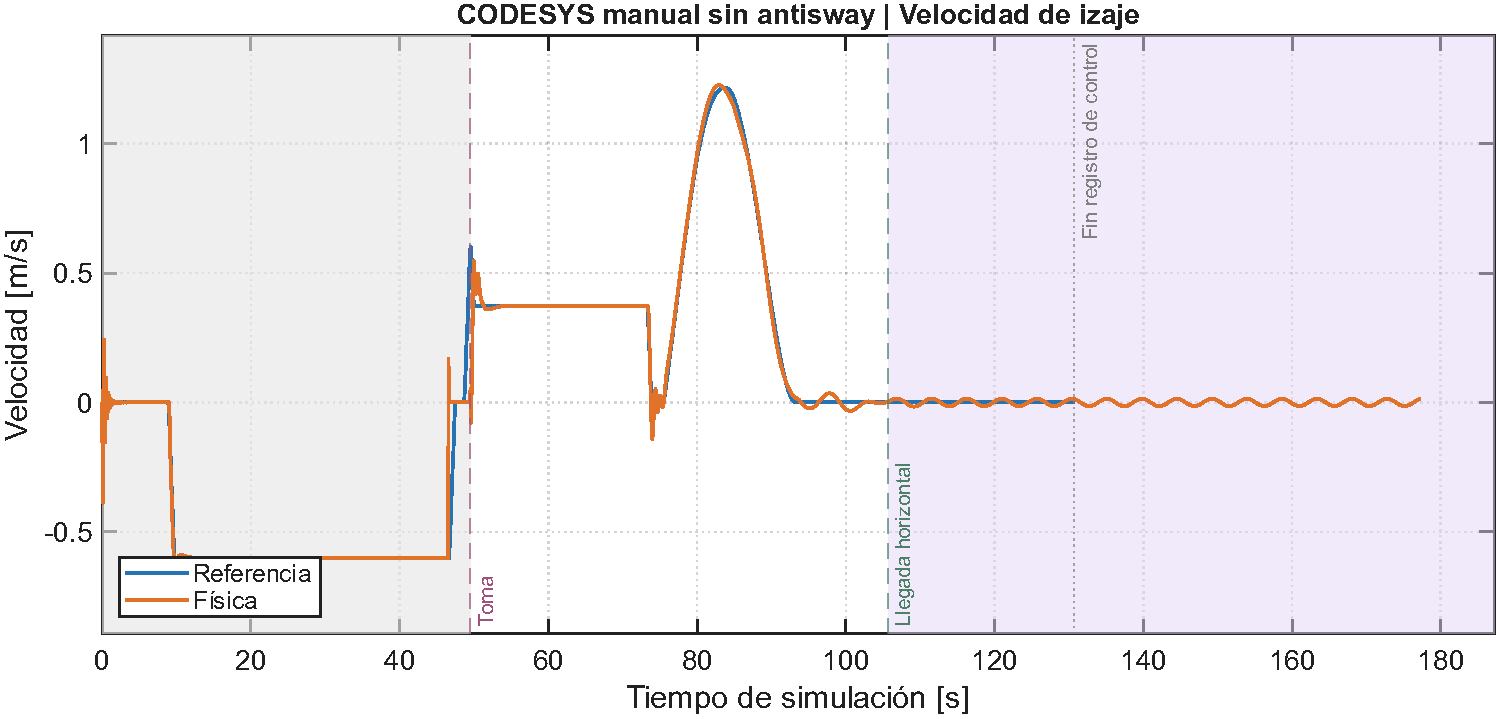
\includegraphics[width=0.98\textwidth]{graficas_individuales/manual_sin_vy.pdf}
\caption{CODESYS manual sin antisway: Velocidad de izaje: referencia y señal física. Se respeta la cobertura parcial de las señales y no se extrapolan datos faltantes.}\label{fig:individual_manual_sin_vy}
\end{figure}

\begin{figure}[!htbp]
\centering
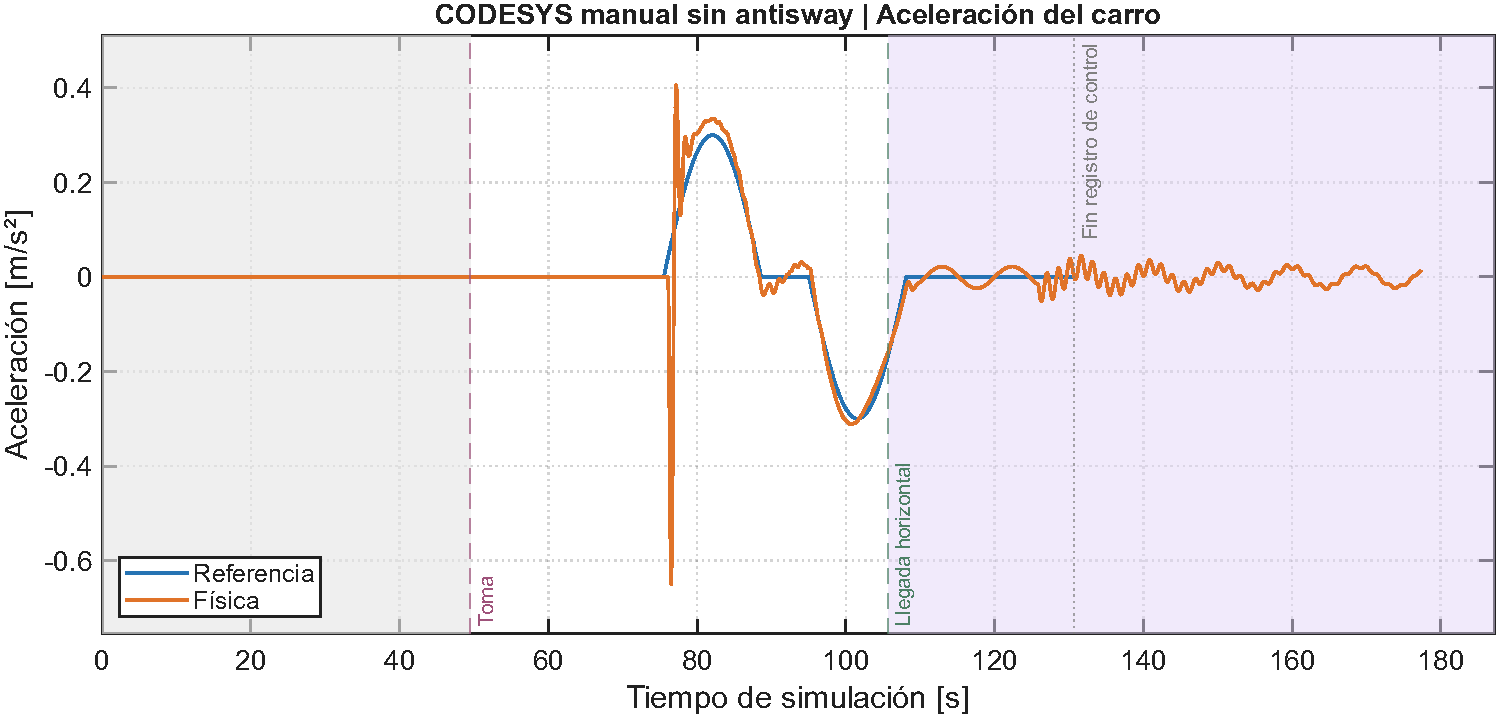
\includegraphics[width=0.98\textwidth]{graficas_individuales/manual_sin_ax.pdf}
\caption{CODESYS manual sin antisway: Aceleración del carro: referencia y señal física. Se respeta la cobertura parcial de las señales y no se extrapolan datos faltantes.}\label{fig:individual_manual_sin_ax}
\end{figure}

\begin{figure}[!htbp]
\centering
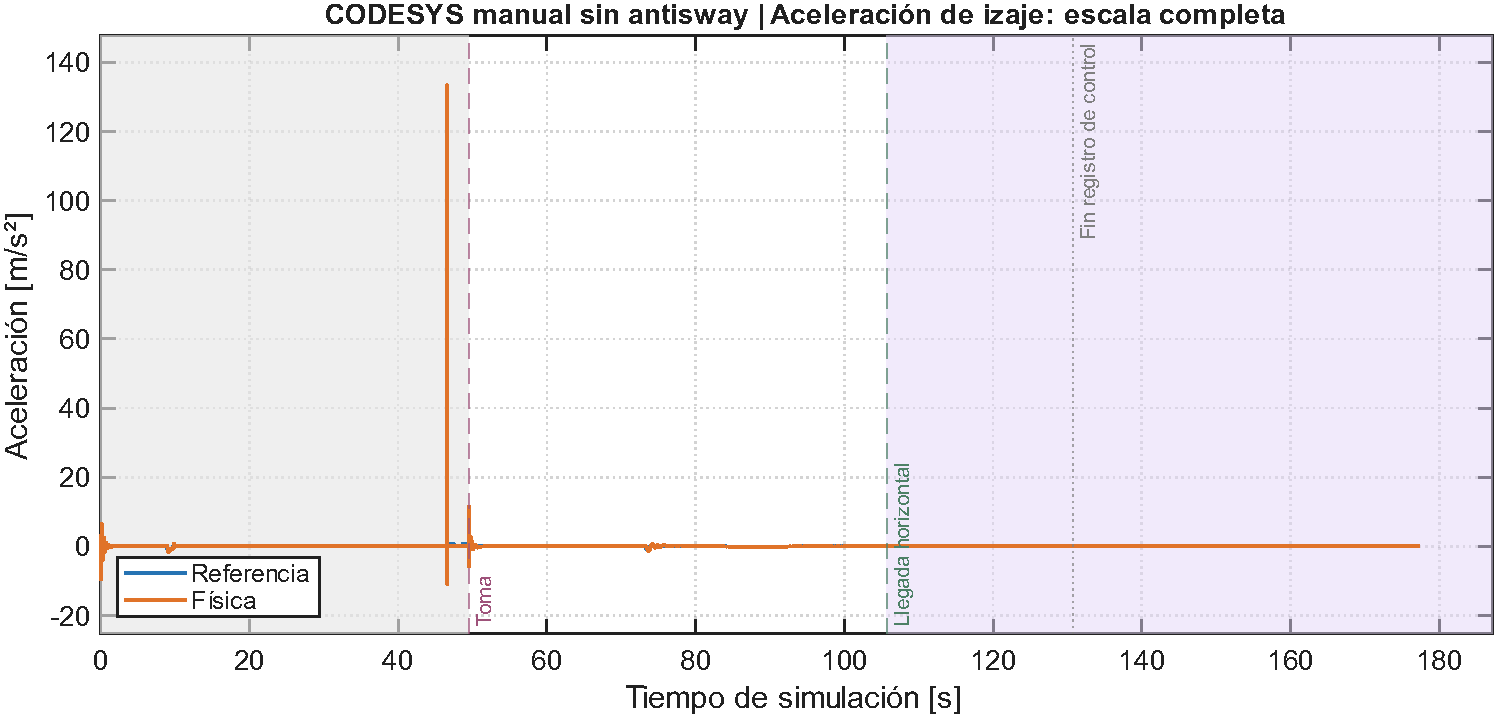
\includegraphics[width=0.98\textwidth]{graficas_individuales/manual_sin_ay.pdf}
\caption{CODESYS manual sin antisway: Aceleración de izaje en escala completa; se conservan los picos de contacto y arranque. Se respeta la cobertura parcial de las señales y no se extrapolan datos faltantes.}\label{fig:individual_manual_sin_ay}
\end{figure}

\begin{figure}[!htbp]
\centering
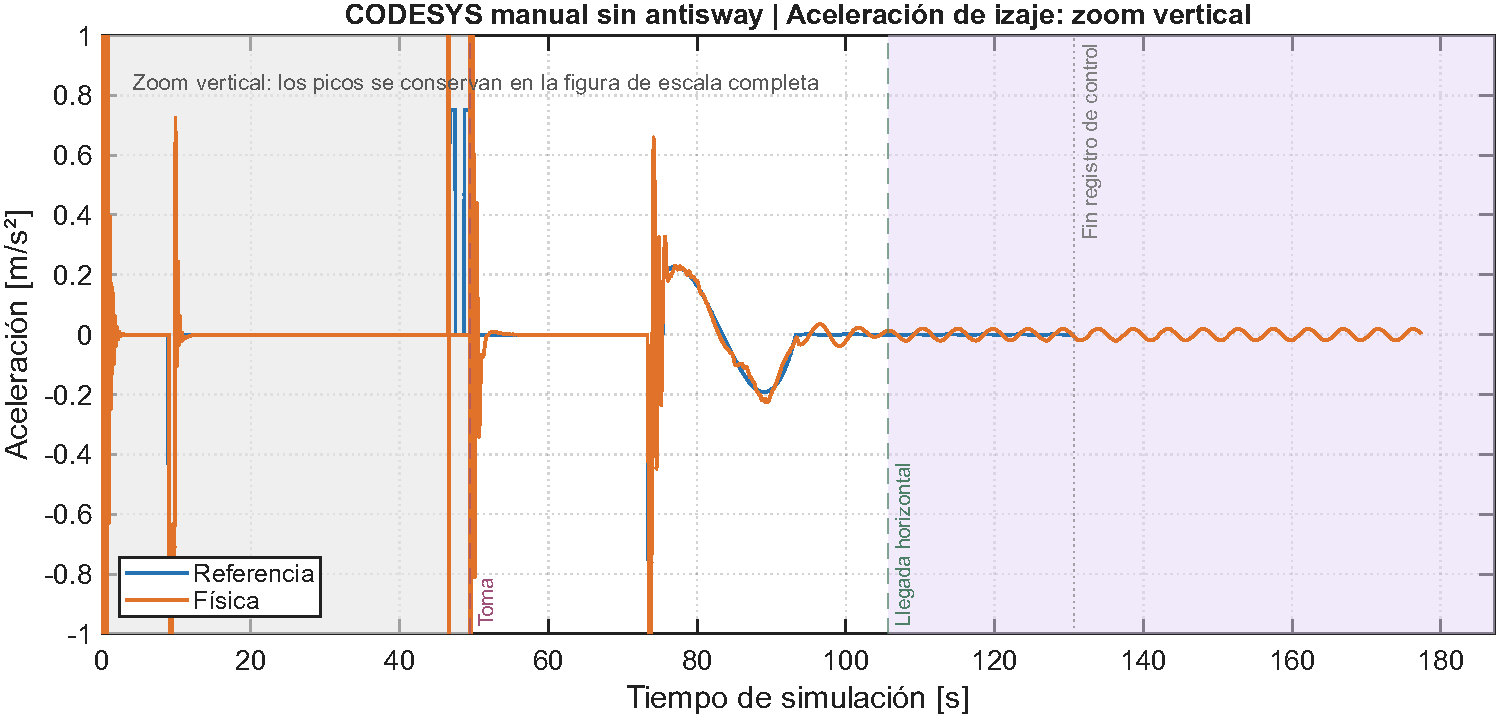
\includegraphics[width=0.98\textwidth]{graficas_individuales/manual_sin_ay_zoom.pdf}
\caption{CODESYS manual sin antisway: Aceleración de izaje con zoom vertical entre $-1$ y $+1~\mathrm{m/s^2}$ para observar su evolución temporal. Los picos que exceden este intervalo permanecen visibles en la figura de escala completa; no se filtraron las señales. Se respeta la cobertura parcial de las señales y no se extrapolan datos faltantes.}\label{fig:individual_manual_sin_ay_zoom}
\end{figure}

El balanceo residual observado es compatible con la espera de la compuerta de estabilidad. En el tramo físico disponible de $120$ a $177.305~\mathrm{s}$, el ángulo RMS fue $0.03169~\mathrm{rad}$ y el máximo absoluto $0.04521~\mathrm{rad}$; la velocidad angular RMS fue $0.02133~\mathrm{rad/s}$ y su máximo $0.03030~\mathrm{rad/s}$. Superar los umbrales angulares en parte de ese tramo no demuestra por sí solo una causa exclusiva del bloqueo. La contribución efectiva y la diferencia entre comando y referencia fueron exactamente cero en el registro nativo disponible hasta $130.72~\mathrm{s}$; no se extiende esa comprobación al tramo faltante.

\begin{figure}[!htbp]
\centering
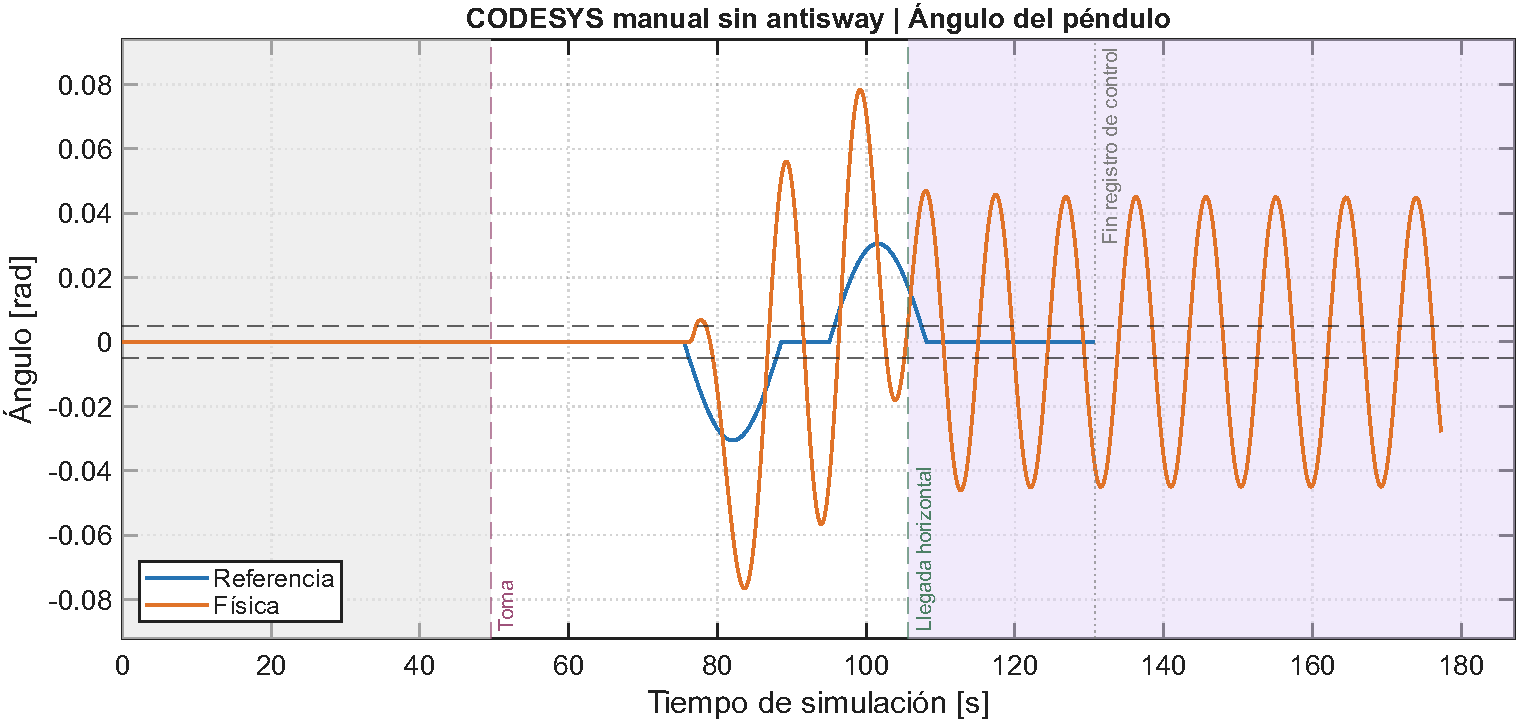
\includegraphics[width=0.98\textwidth]{graficas_individuales/manual_sin_theta.pdf}
\caption{CODESYS manual sin antisway: Ángulo físico y de referencia del péndulo. Las líneas horizontales señalan los umbrales angulares del descenso. Se respeta la cobertura parcial de las señales y no se extrapolan datos faltantes.}\label{fig:individual_manual_sin_theta}
\end{figure}

\begin{figure}[!htbp]
\centering
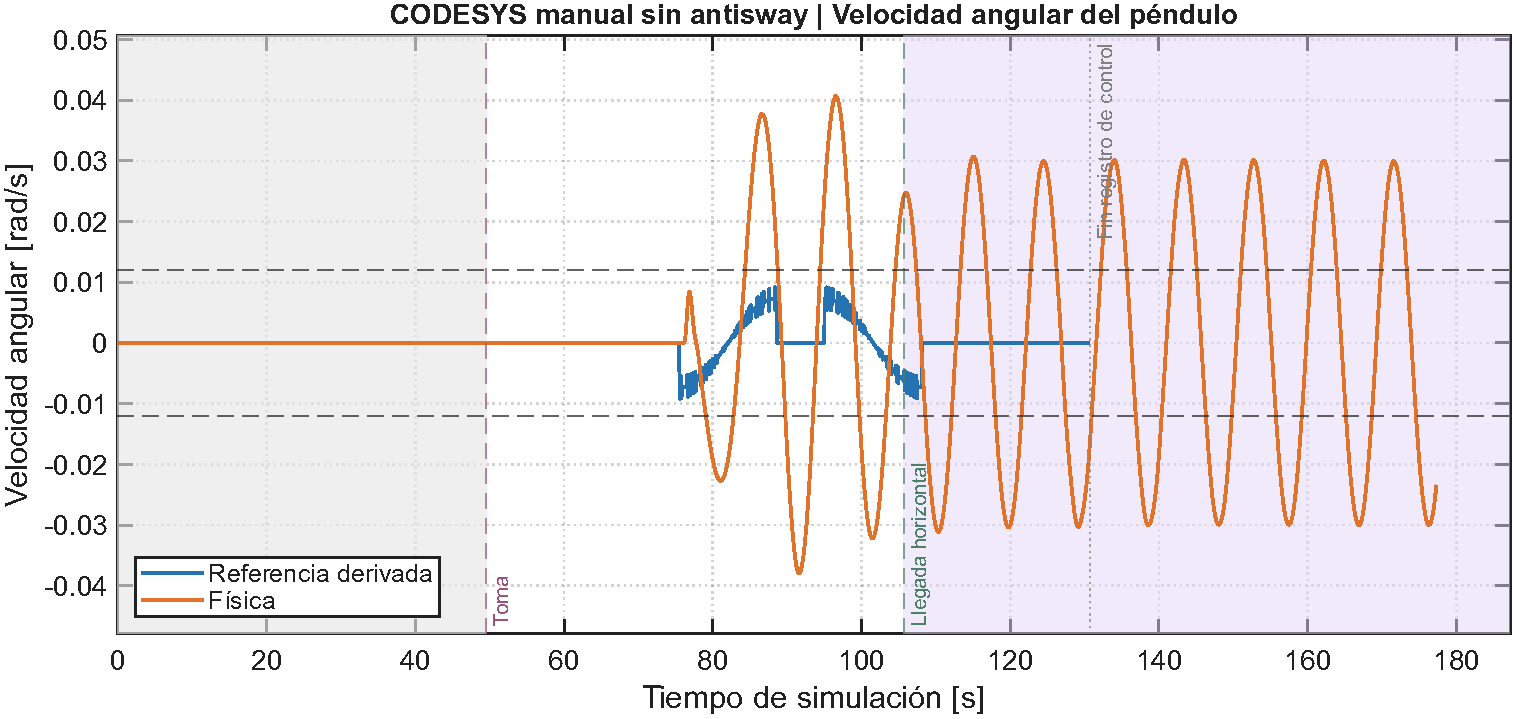
\includegraphics[width=0.98\textwidth]{graficas_individuales/manual_sin_omega.pdf}
\caption{CODESYS manual sin antisway: Velocidad angular física y referencia derivada numéricamente; se distinguen ambas fuentes. Las líneas horizontales indican los umbrales del descenso. Se respeta la cobertura parcial de las señales y no se extrapolan datos faltantes.}\label{fig:individual_manual_sin_omega}
\end{figure}

\begin{figure}[!htbp]
\centering
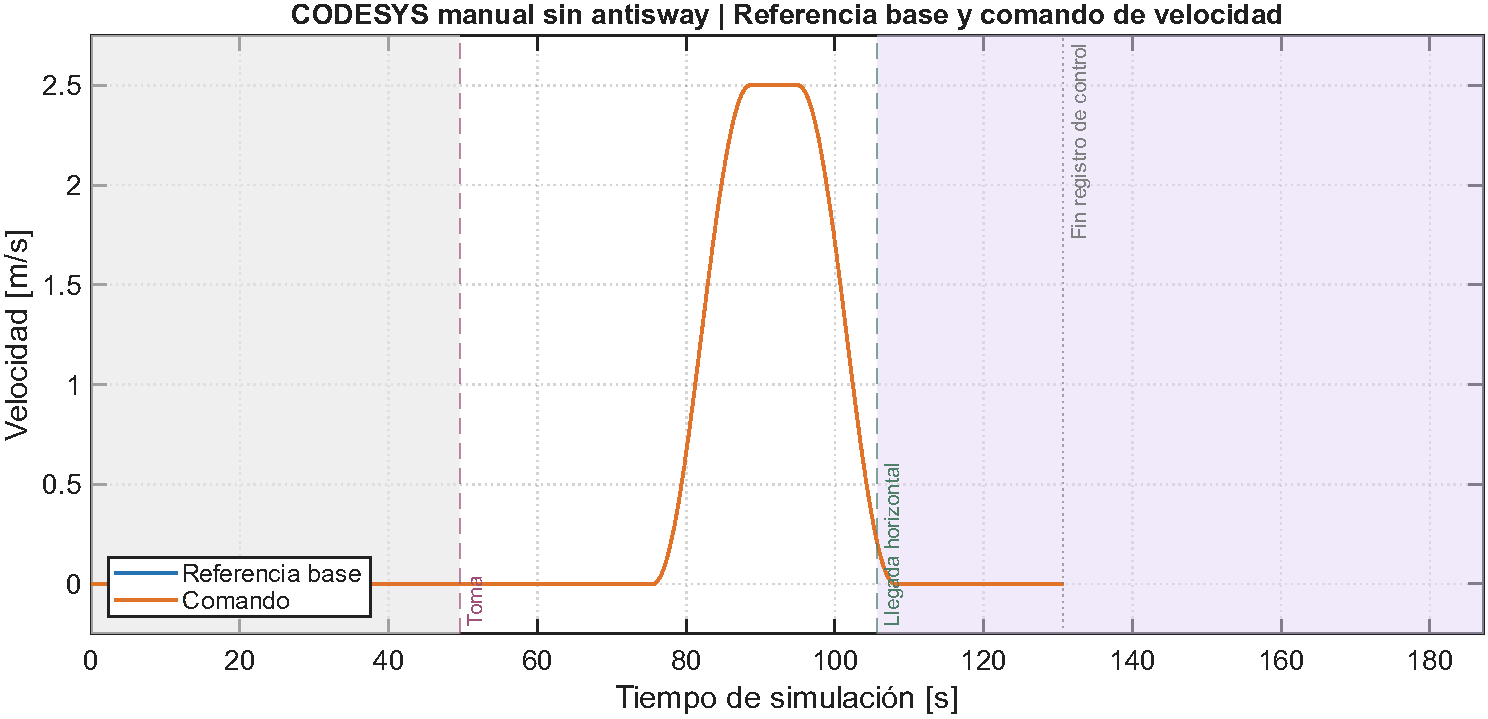
\includegraphics[width=0.98\textwidth]{graficas_individuales/manual_sin_vcmd.pdf}
\caption{CODESYS manual sin antisway: Referencia base y comando de velocidad; su diferencia corresponde a la contribución antisway efectiva en el sumador. Se respeta la cobertura parcial de las señales y no se extrapolan datos faltantes.}\label{fig:individual_manual_sin_vcmd}
\end{figure}

\begin{figure}[!htbp]
\centering
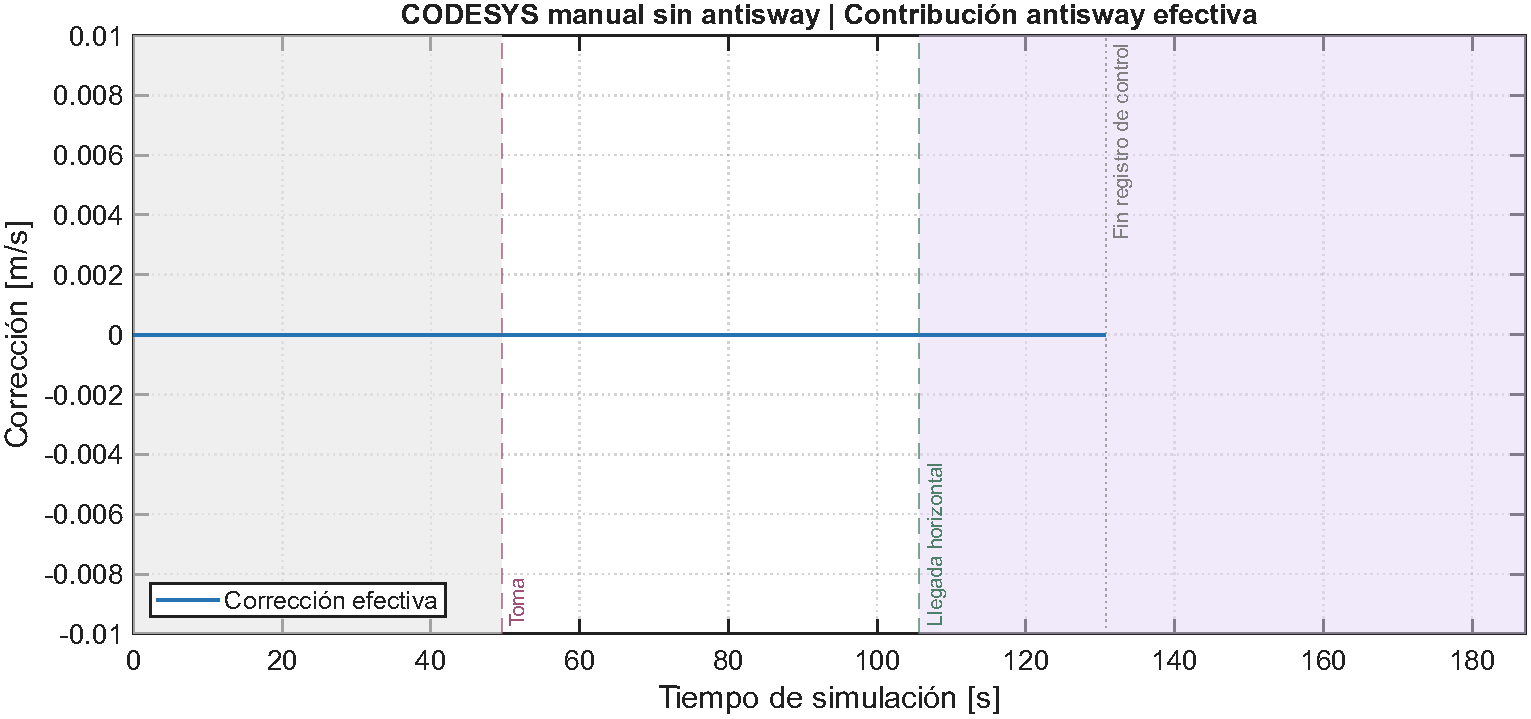
\includegraphics[width=0.98\textwidth]{graficas_individuales/manual_sin_sw.pdf}
\caption{CODESYS manual sin antisway: Contribución antisway efectivamente sumada al comando de velocidad. Se respeta la cobertura parcial de las señales y no se extrapolan datos faltantes.}\label{fig:individual_manual_sin_sw}
\end{figure}

Los torques diferencian la consigna del controlador y el torque físico de motor; su diferencia y los transitorios no se eliminan con filtrado posterior. Se muestra el arranque completo y una ampliación desde START para evitar que un pico inicial oculte el resto de la maniobra. La tensión permanece asociada a la carga suspendida en el tramo registrado. Los errores de posición se calculan sólo dentro de la cobertura común de referencia y señal física.

\begin{figure}[!htbp]
\centering
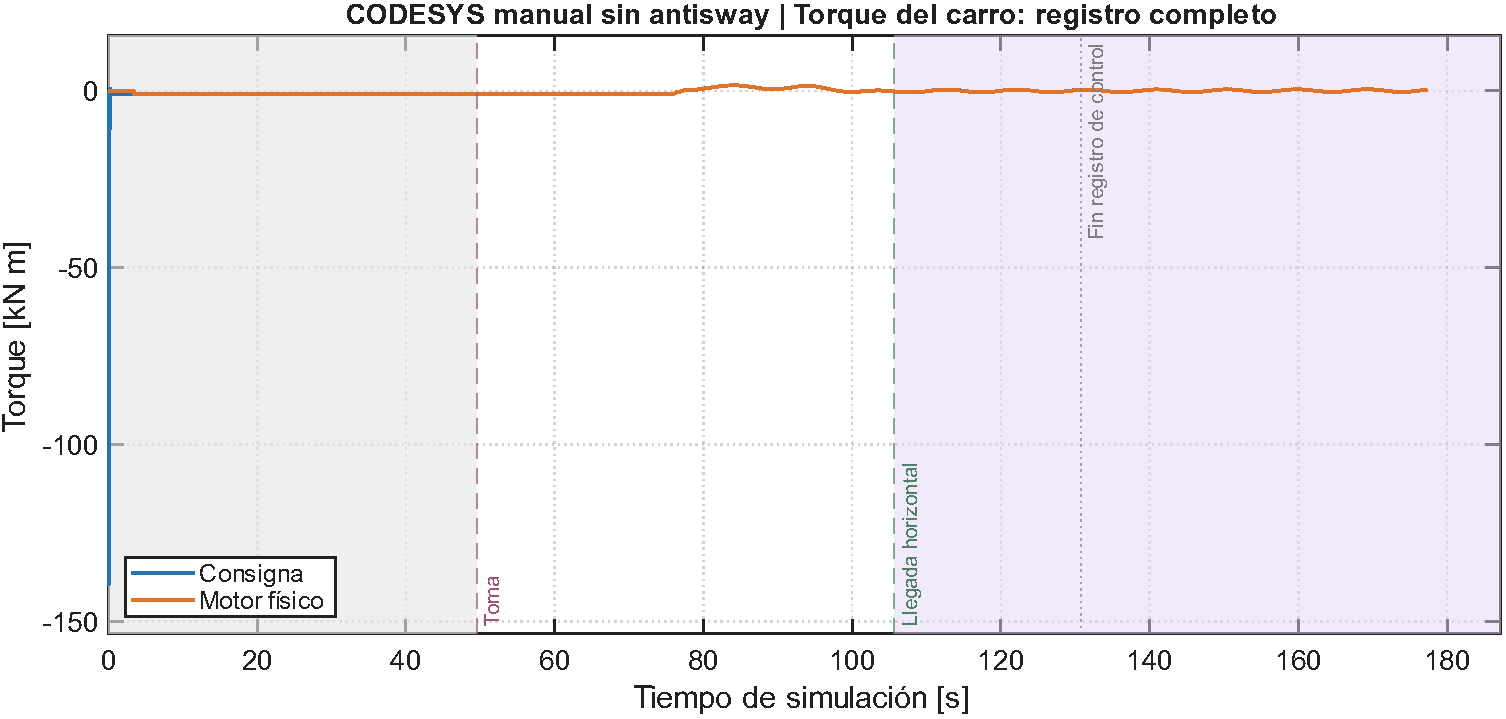
\includegraphics[width=0.98\textwidth]{graficas_individuales/manual_sin_tx.pdf}
\caption{CODESYS manual sin antisway: Consigna y torque físico del motor del carro en el intervalo representado, incluido el arranque.}\label{fig:individual_manual_sin_tx}
\end{figure}

\begin{figure}[!htbp]
\centering
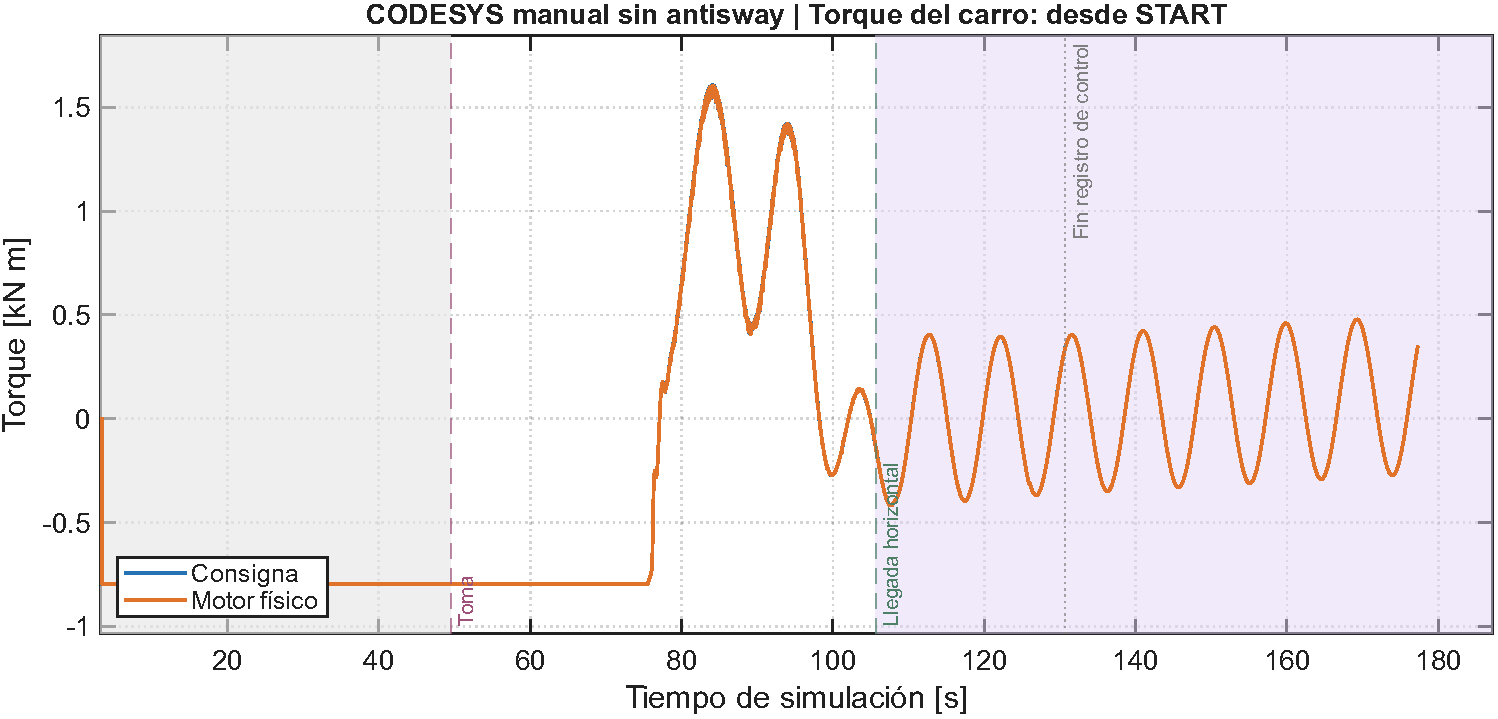
\includegraphics[width=0.98\textwidth]{graficas_individuales/manual_sin_tx_zoom.pdf}
\caption{CODESYS manual sin antisway: Consigna y torque físico del motor del carro desde START; la escala completa del arranque se conserva en una figura independiente.}\label{fig:individual_manual_sin_tx_zoom}
\end{figure}

\begin{figure}[!htbp]
\centering
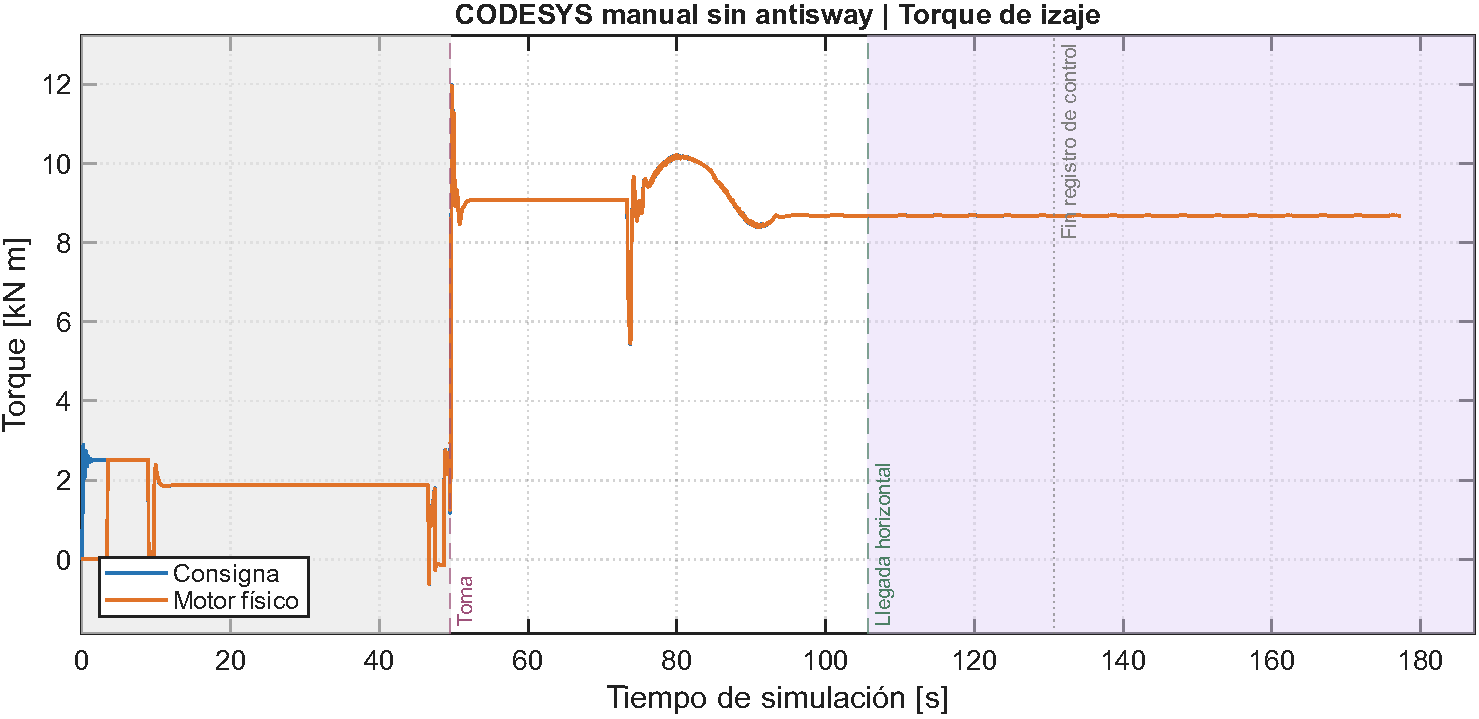
\includegraphics[width=0.98\textwidth]{graficas_individuales/manual_sin_ty.pdf}
\caption{CODESYS manual sin antisway: Consigna del controlador y torque físico del motor de izaje.}\label{fig:individual_manual_sin_ty}
\end{figure}

\begin{figure}[!htbp]
\centering
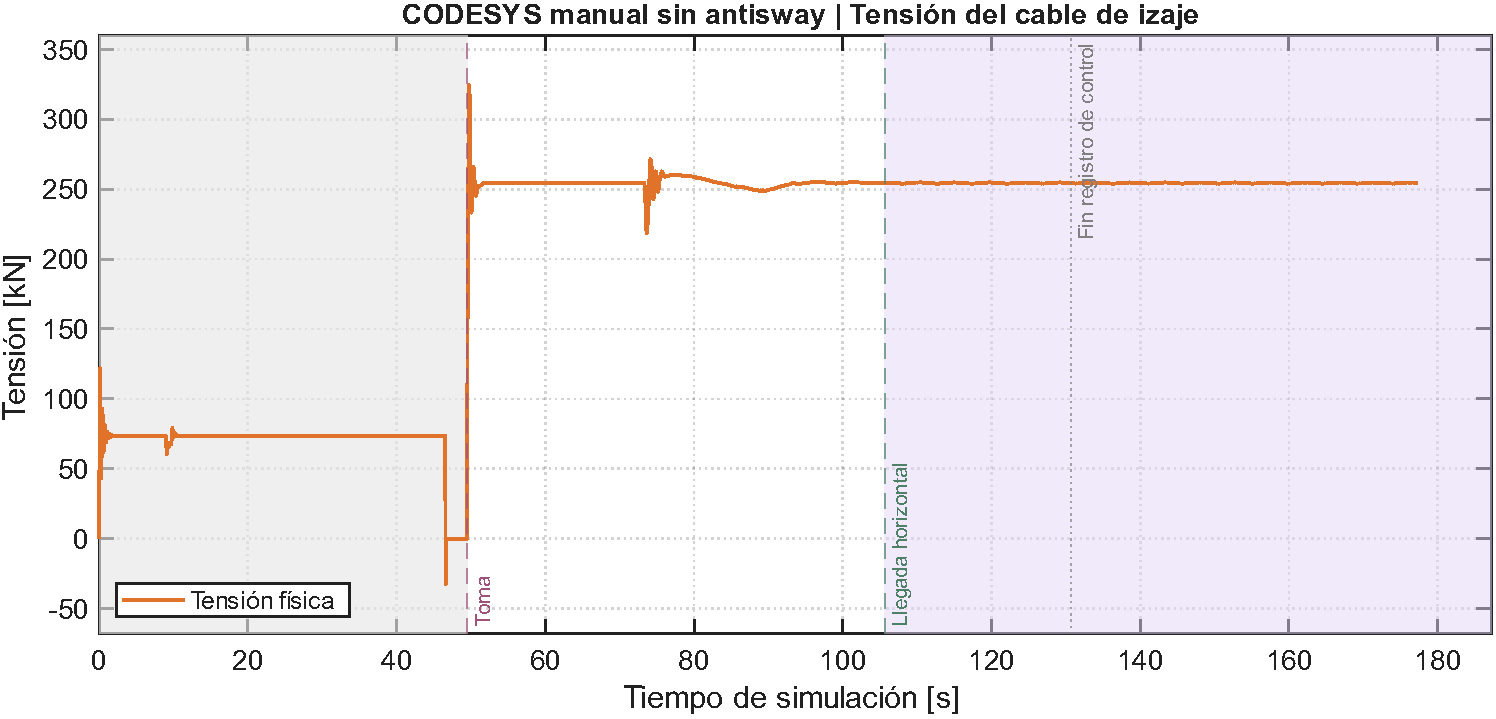
\includegraphics[width=0.98\textwidth]{graficas_individuales/manual_sin_tension.pdf}
\caption{CODESYS manual sin antisway: Tensión física del cable de izaje.}\label{fig:individual_manual_sin_tension}
\end{figure}

\begin{figure}[!htbp]
\centering
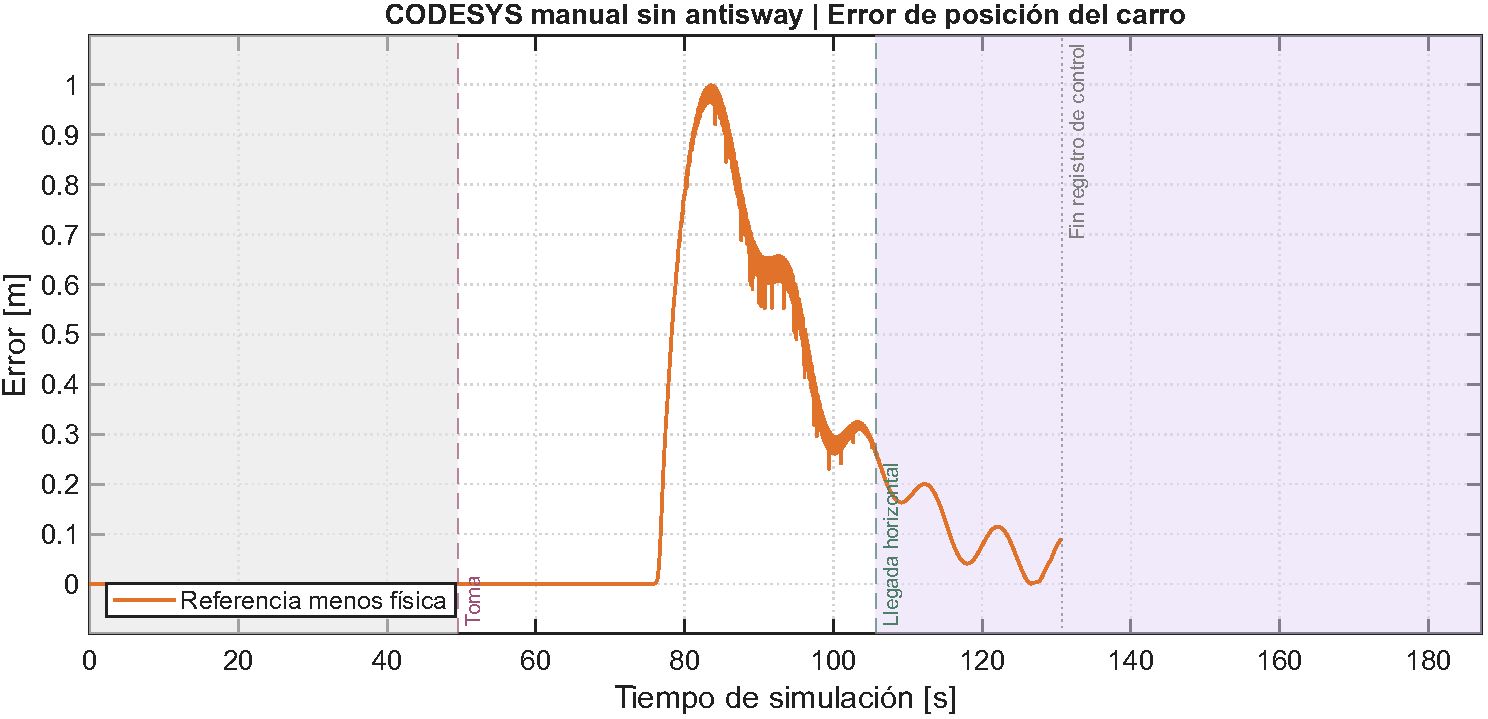
\includegraphics[width=0.98\textwidth]{graficas_individuales/manual_sin_ex.pdf}
\caption{CODESYS manual sin antisway: Error horizontal, calculado como referencia menos posición física. Se respeta la cobertura parcial de las señales y no se extrapolan datos faltantes.}\label{fig:individual_manual_sin_ex}
\end{figure}

\begin{figure}[!htbp]
\centering
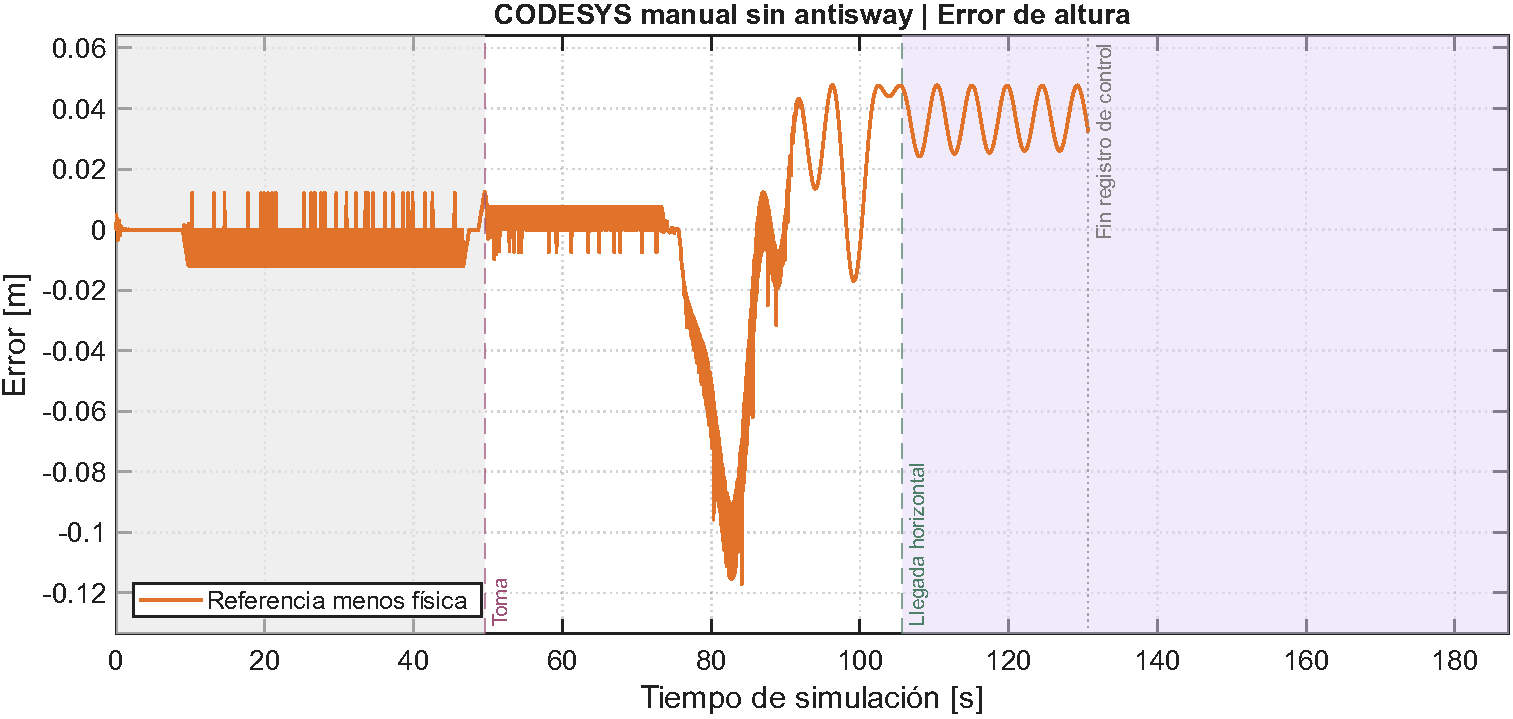
\includegraphics[width=0.98\textwidth]{graficas_individuales/manual_sin_ey.pdf}
\caption{CODESYS manual sin antisway: Error de altura, calculado como referencia menos altura física. Se respeta la cobertura parcial de las señales y no se extrapolan datos faltantes.}\label{fig:individual_manual_sin_ey}
\end{figure}

\begin{figure}[!htbp]
\centering
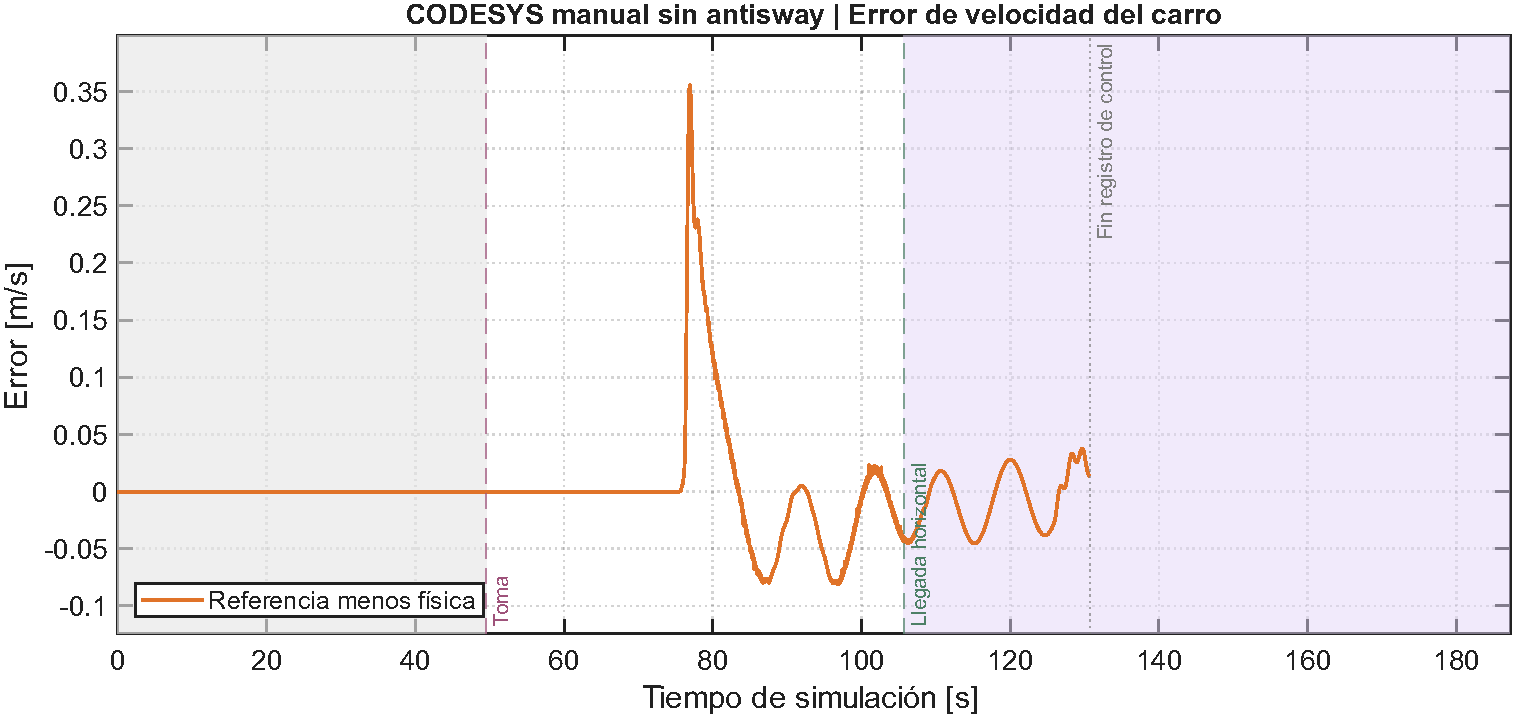
\includegraphics[width=0.98\textwidth]{graficas_individuales/manual_sin_evx.pdf}
\caption{CODESYS manual sin antisway: Error de velocidad del carro, calculado como referencia menos velocidad física. Se respeta la cobertura parcial de las señales y no se extrapolan datos faltantes.}\label{fig:individual_manual_sin_evx}
\end{figure}

\begin{figure}[!htbp]
\centering
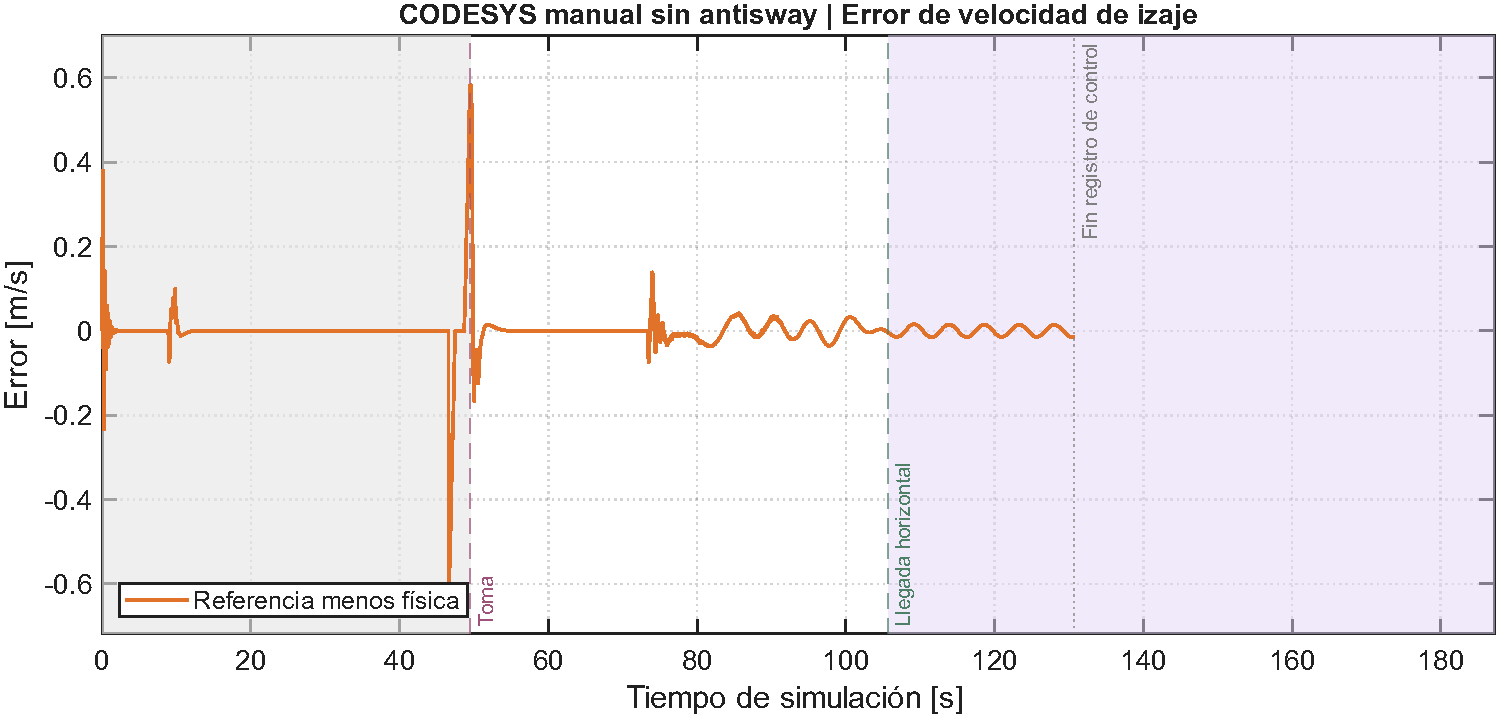
\includegraphics[width=0.98\textwidth]{graficas_individuales/manual_sin_evy.pdf}
\caption{CODESYS manual sin antisway: Error de velocidad de izaje, calculado como referencia menos velocidad física. Se respeta la cobertura parcial de las señales y no se extrapolan datos faltantes.}\label{fig:individual_manual_sin_evy}
\end{figure}

\begin{figure}[!htbp]
\centering
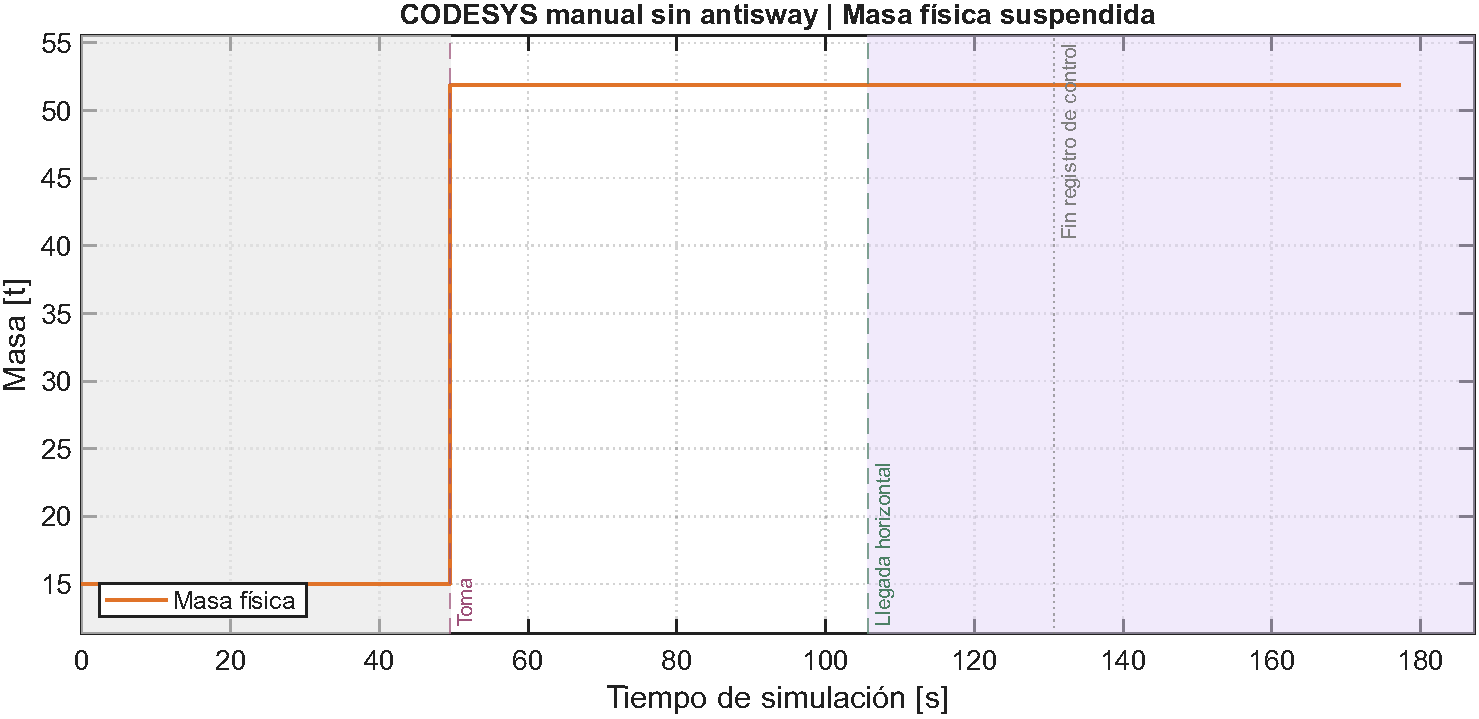
\includegraphics[width=0.98\textwidth]{graficas_individuales/manual_sin_masa.pdf}
\caption{CODESYS manual sin antisway: Masa física suspendida: 51,863 t representa conjunto cargado y 15 t corresponde al spreader vacío.}\label{fig:individual_manual_sin_masa}
\end{figure}

\begin{figure}[!htbp]
\centering
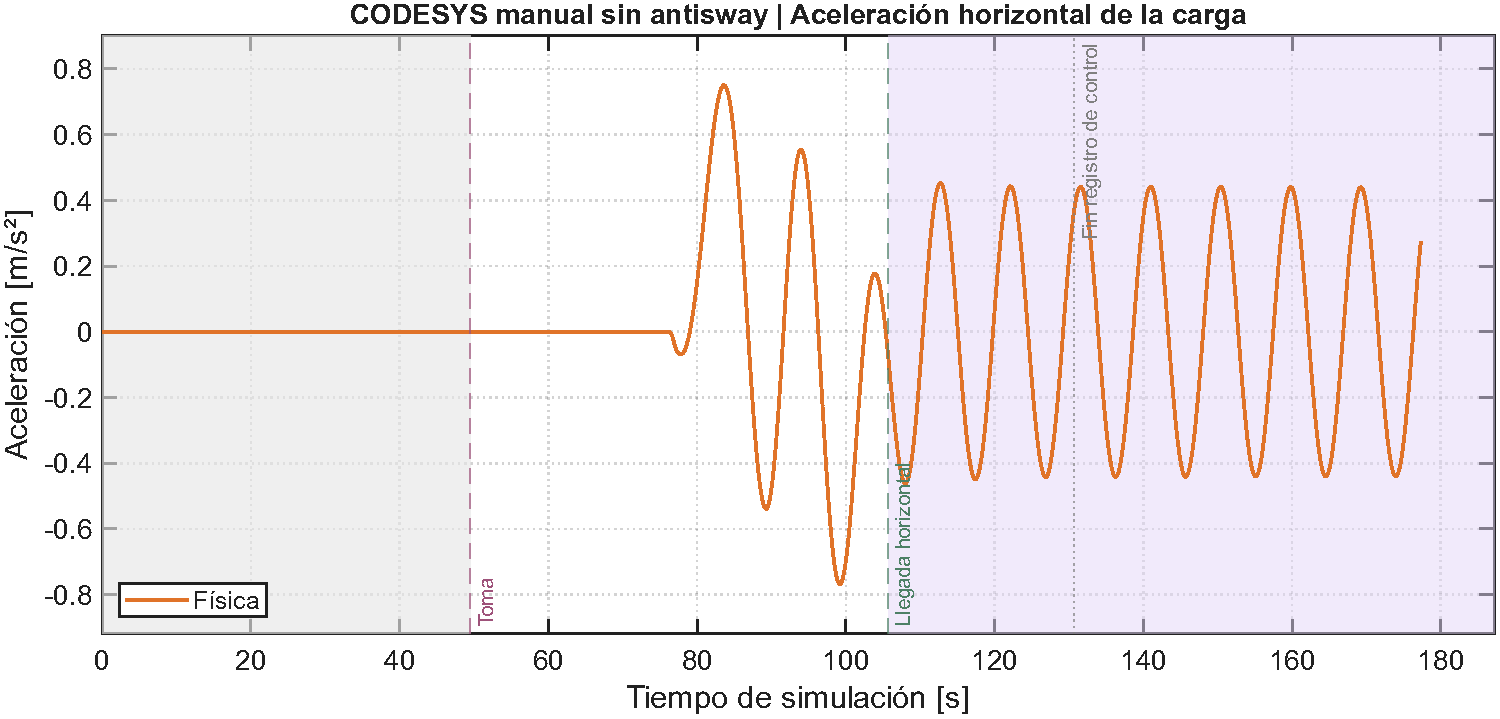
\includegraphics[width=0.98\textwidth]{graficas_individuales/manual_sin_ax_carga.pdf}
\caption{CODESYS manual sin antisway: Aceleración horizontal física de la carga; se conservan las oscilaciones registradas.}\label{fig:individual_manual_sin_ax_carga}
\end{figure}

\clearpage
\subsection{CODESYS manual con antisway: entrega física completada}
La secuencia inicial fue equivalente: START a $3.24~\mathrm{s}$, manual a $3.76~\mathrm{s}$, cierre solicitado a $46.64~\mathrm{s}$, masa cargada a $49.56~\mathrm{s}$ y despegue físico a $50.04~\mathrm{s}$. Automático se solicitó a $75.32~\mathrm{s}$ y fue observado por el operador a $75.44~\mathrm{s}$. La llegada horizontal ocurrió a $105.84~\mathrm{s}$; manual se solicitó a $133.24~\mathrm{s}$ y se observó a $133.32~\mathrm{s}$. El apoyo y apertura se solicitaron a $168.92~\mathrm{s}$, la entrega y STOP a $169.12~\mathrm{s}$, y la simulación terminó a $169.20~\mathrm{s}$.

Las posiciones y velocidades describen el cruce, el descenso automático habilitado y la aproximación manual final. Los picos de aceleración próximos al contacto pertenecen a la dinámica de apoyo y no se recortan. La corrección antisway modifica el comando respecto de la referencia base y reduce el balanceo hasta permitir el avance de la secuencia; su máximo nativo fue $0.46245~\mathrm{m/s}$. Esto no implica que todos los errores máximos de seguimiento sean menores.

\begin{figure}[!htbp]
\centering
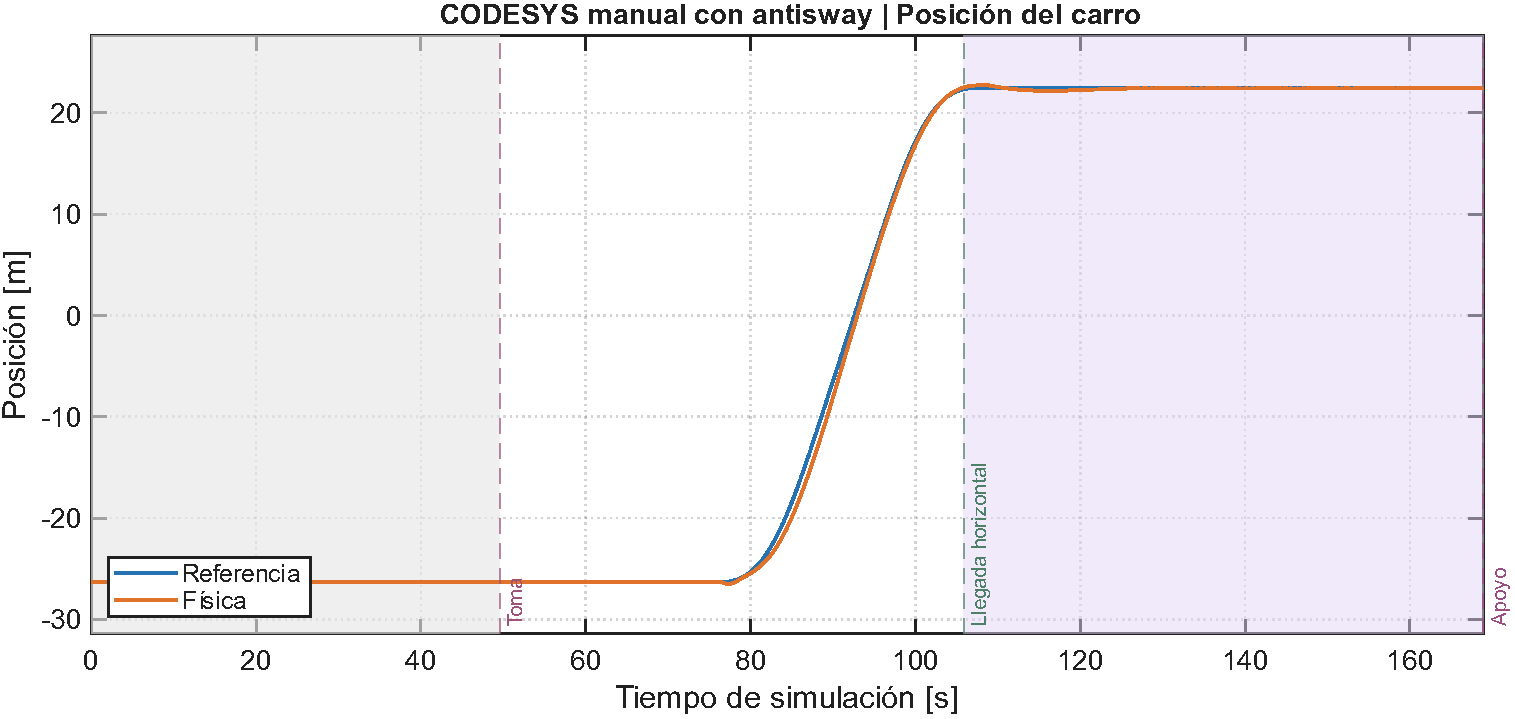
\includegraphics[width=0.98\textwidth]{graficas_individuales/manual_con_x.pdf}
\caption{CODESYS manual con antisway: Posición del carro: referencia y evolución física.}\label{fig:individual_manual_con_x}
\end{figure}

\begin{figure}[!htbp]
\centering
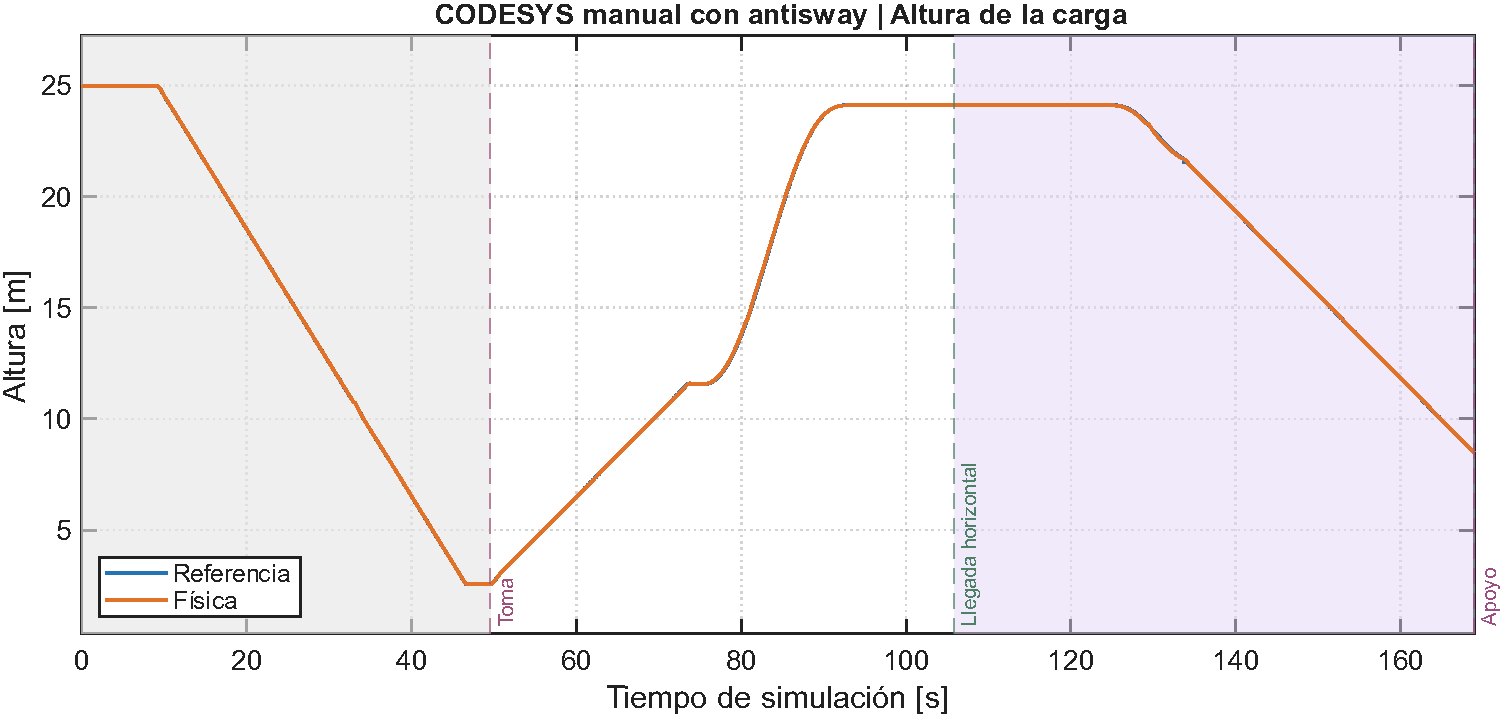
\includegraphics[width=0.98\textwidth]{graficas_individuales/manual_con_y.pdf}
\caption{CODESYS manual con antisway: Altura de la carga: referencia y evolución física.}\label{fig:individual_manual_con_y}
\end{figure}

\begin{figure}[!htbp]
\centering
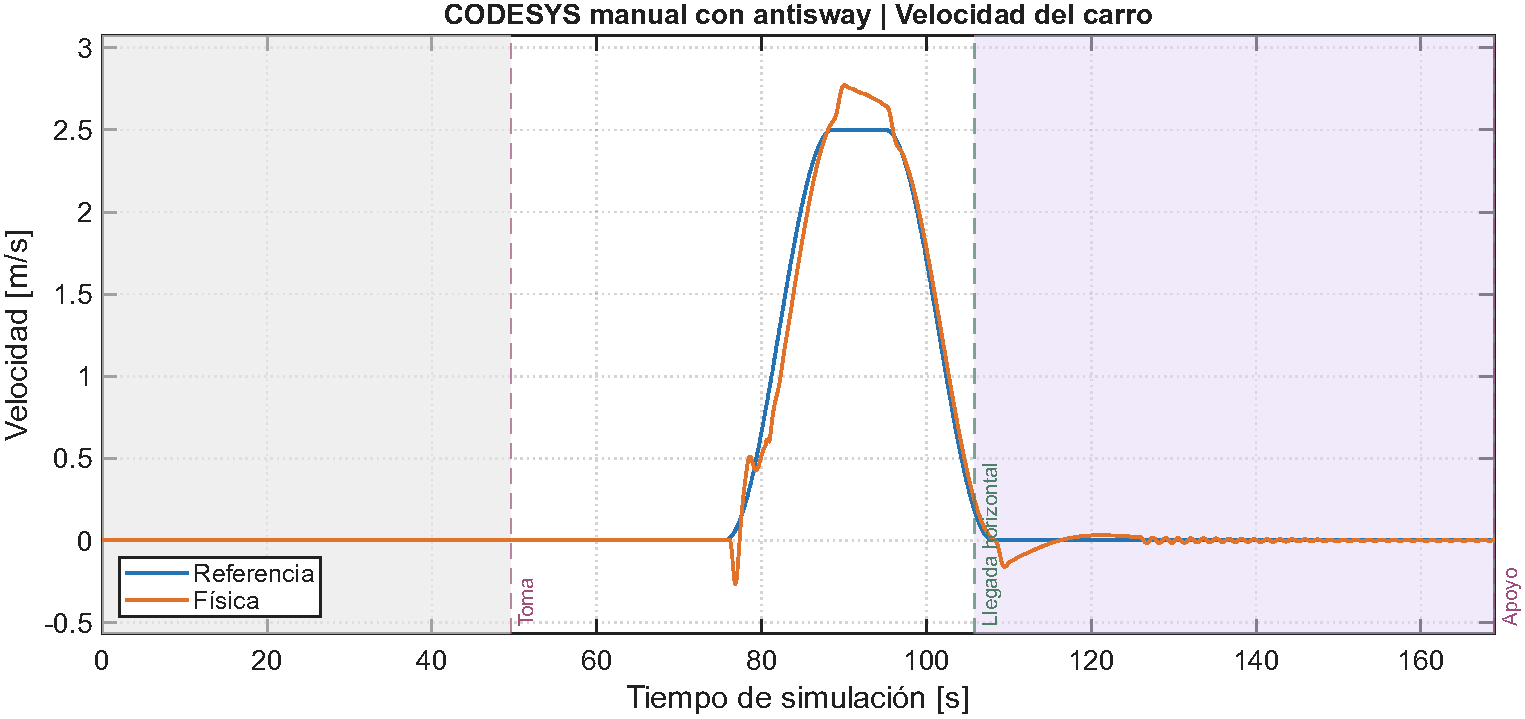
\includegraphics[width=0.98\textwidth]{graficas_individuales/manual_con_vx.pdf}
\caption{CODESYS manual con antisway: Velocidad del carro: referencia y señal física.}\label{fig:individual_manual_con_vx}
\end{figure}

\begin{figure}[!htbp]
\centering
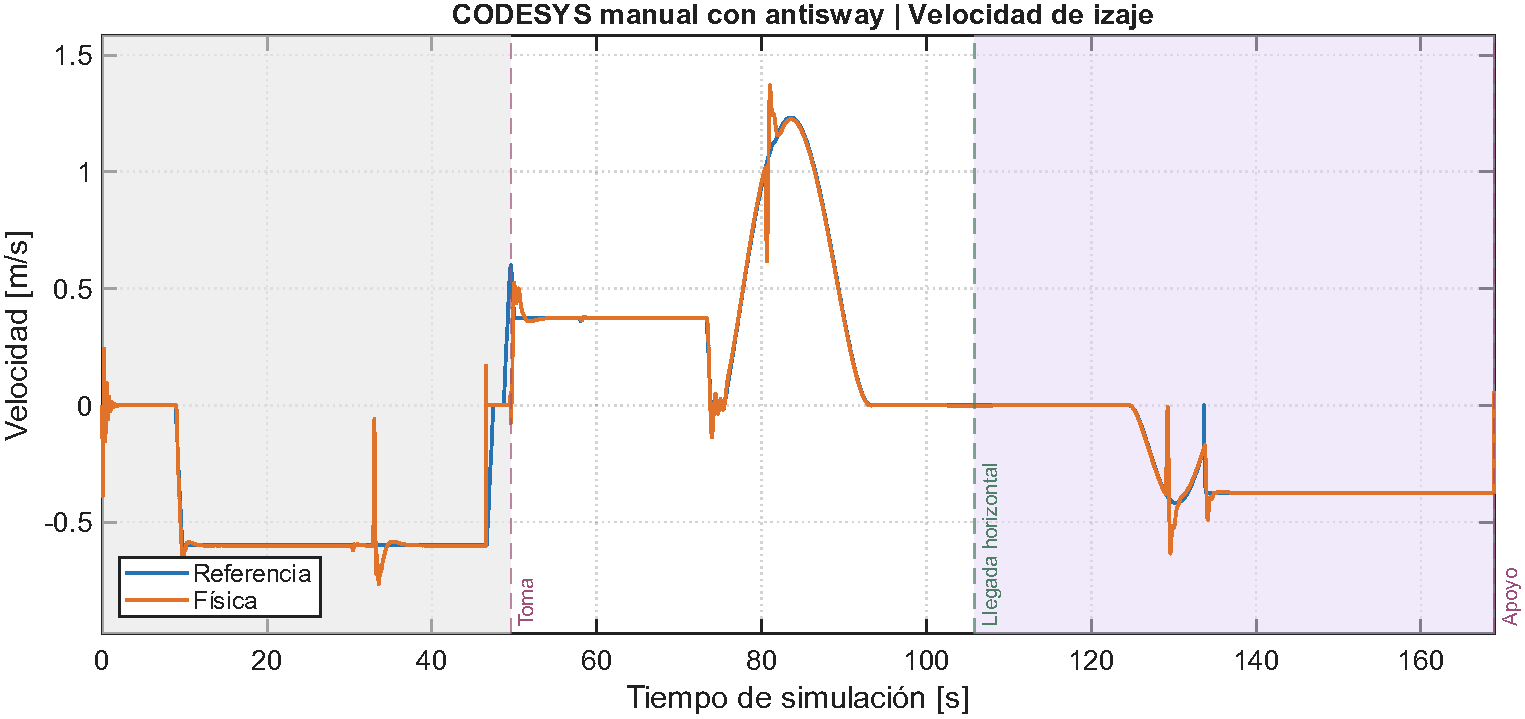
\includegraphics[width=0.98\textwidth]{graficas_individuales/manual_con_vy.pdf}
\caption{CODESYS manual con antisway: Velocidad de izaje: referencia y señal física.}\label{fig:individual_manual_con_vy}
\end{figure}

\begin{figure}[!htbp]
\centering
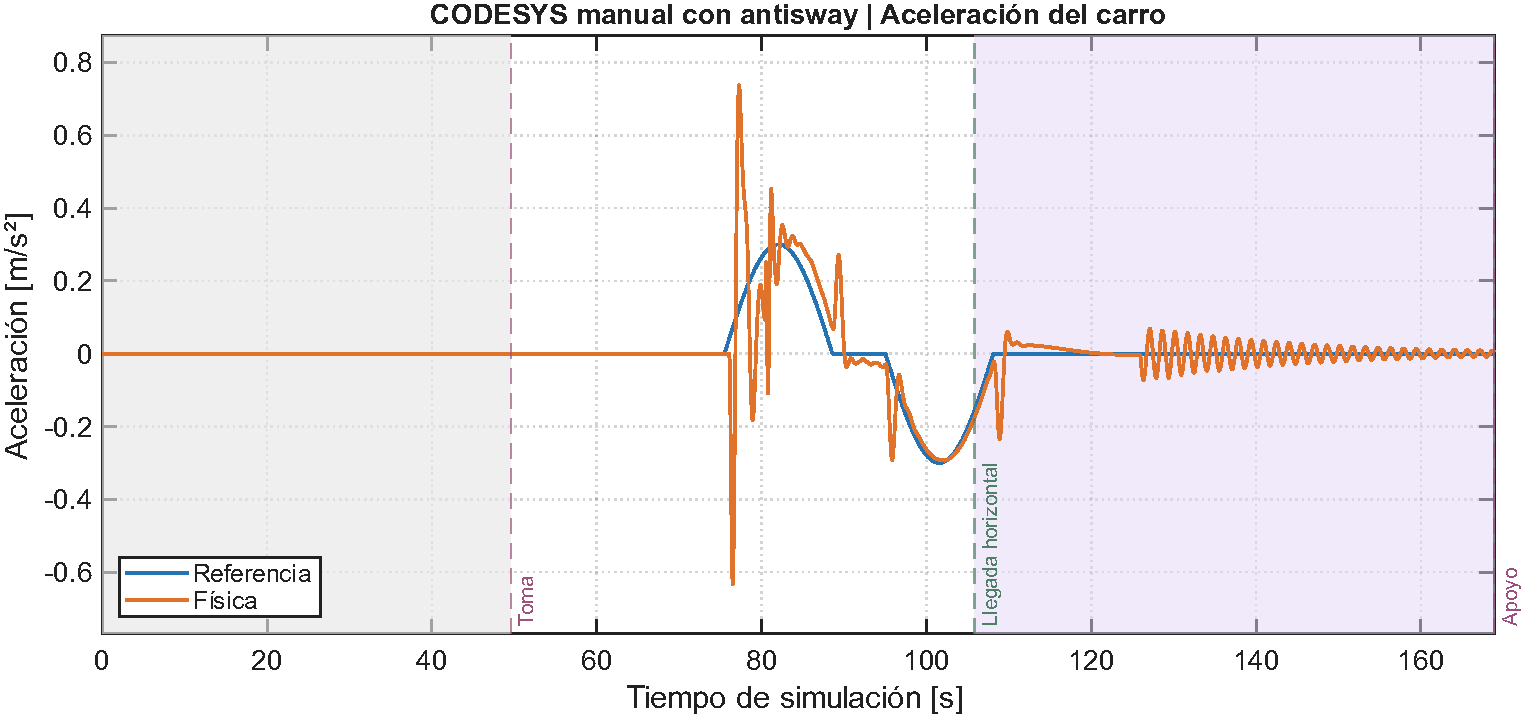
\includegraphics[width=0.98\textwidth]{graficas_individuales/manual_con_ax.pdf}
\caption{CODESYS manual con antisway: Aceleración del carro: referencia y señal física.}\label{fig:individual_manual_con_ax}
\end{figure}

\begin{figure}[!htbp]
\centering
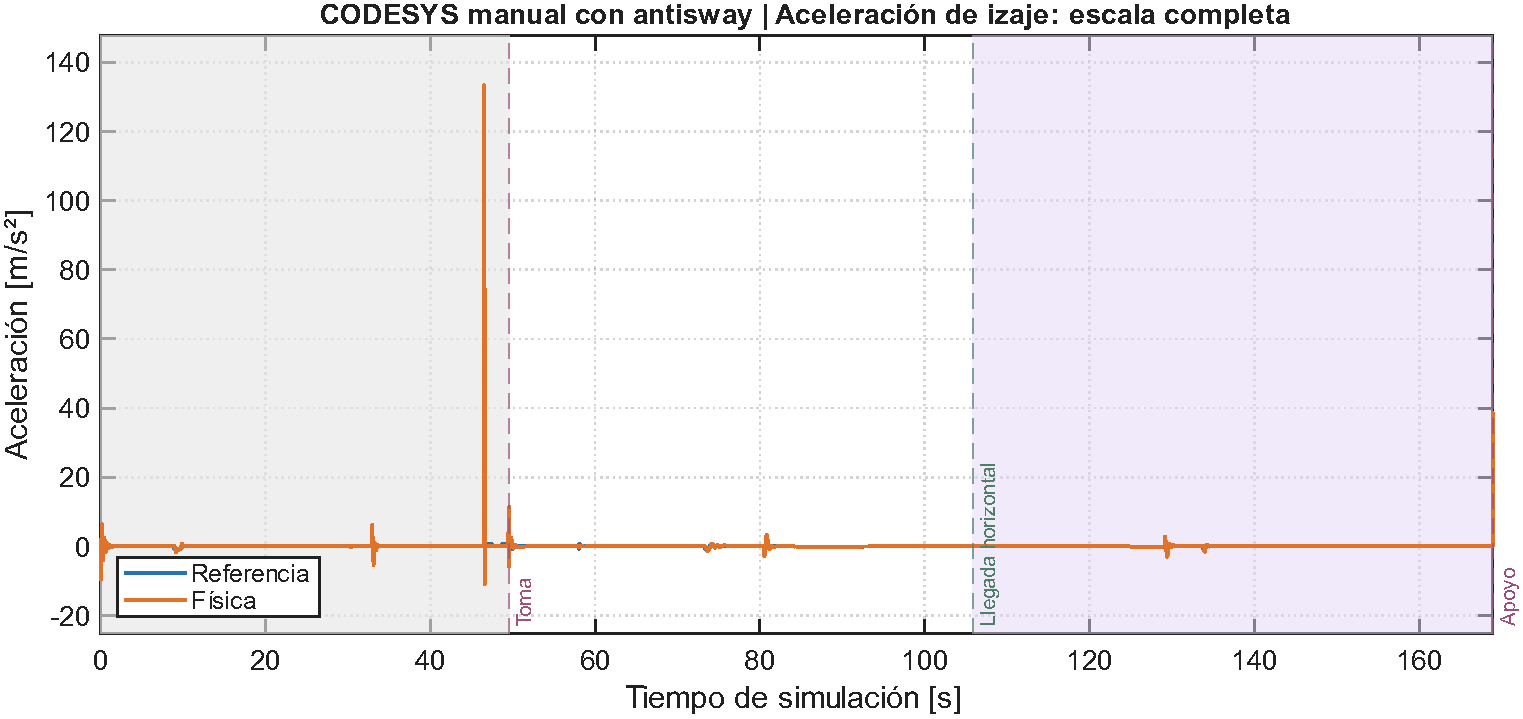
\includegraphics[width=0.98\textwidth]{graficas_individuales/manual_con_ay.pdf}
\caption{CODESYS manual con antisway: Aceleración de izaje en escala completa; se conservan los picos de contacto y arranque.}\label{fig:individual_manual_con_ay}
\end{figure}

\begin{figure}[!htbp]
\centering
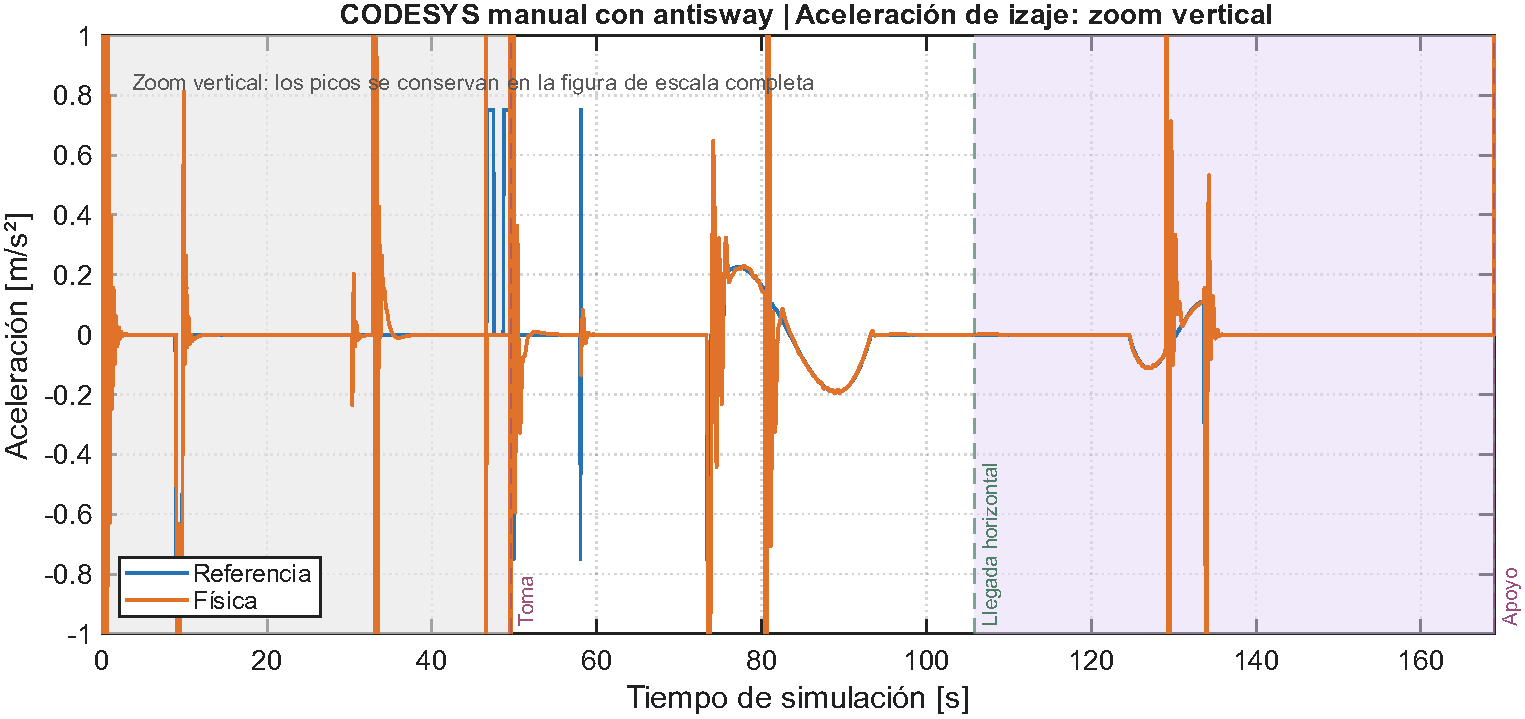
\includegraphics[width=0.98\textwidth]{graficas_individuales/manual_con_ay_zoom.pdf}
\caption{CODESYS manual con antisway: Aceleración de izaje con zoom vertical entre $-1$ y $+1~\mathrm{m/s^2}$ para observar su evolución temporal. Los picos que exceden este intervalo permanecen visibles en la figura de escala completa; no se filtraron las señales.}\label{fig:individual_manual_con_ay_zoom}
\end{figure}

\begin{figure}[!htbp]
\centering
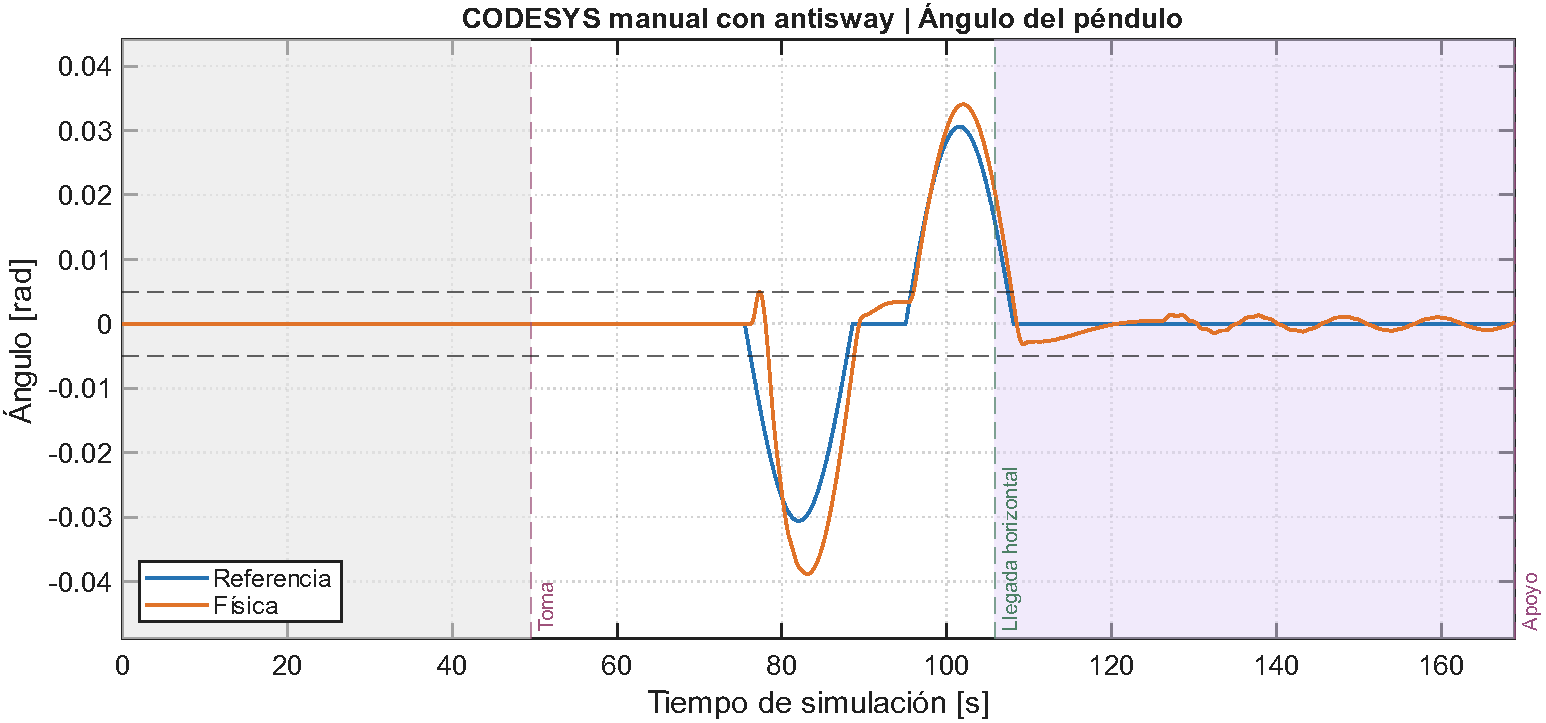
\includegraphics[width=0.98\textwidth]{graficas_individuales/manual_con_theta.pdf}
\caption{CODESYS manual con antisway: Ángulo físico y de referencia del péndulo. Las líneas horizontales señalan los umbrales angulares del descenso.}\label{fig:individual_manual_con_theta}
\end{figure}

\begin{figure}[!htbp]
\centering
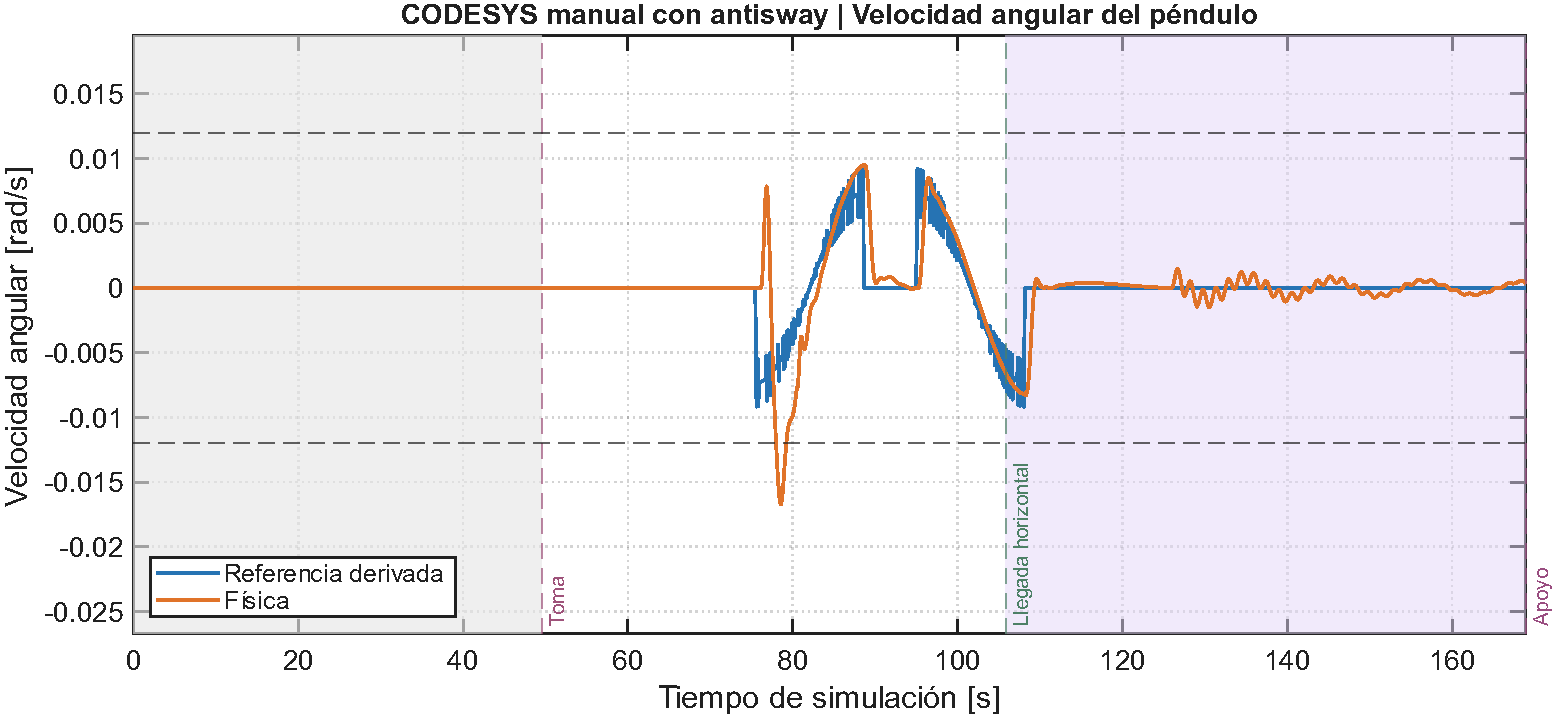
\includegraphics[width=0.98\textwidth]{graficas_individuales/manual_con_omega.pdf}
\caption{CODESYS manual con antisway: Velocidad angular física y referencia derivada numéricamente; se distinguen ambas fuentes. Las líneas horizontales indican los umbrales del descenso.}\label{fig:individual_manual_con_omega}
\end{figure}

\begin{figure}[!htbp]
\centering
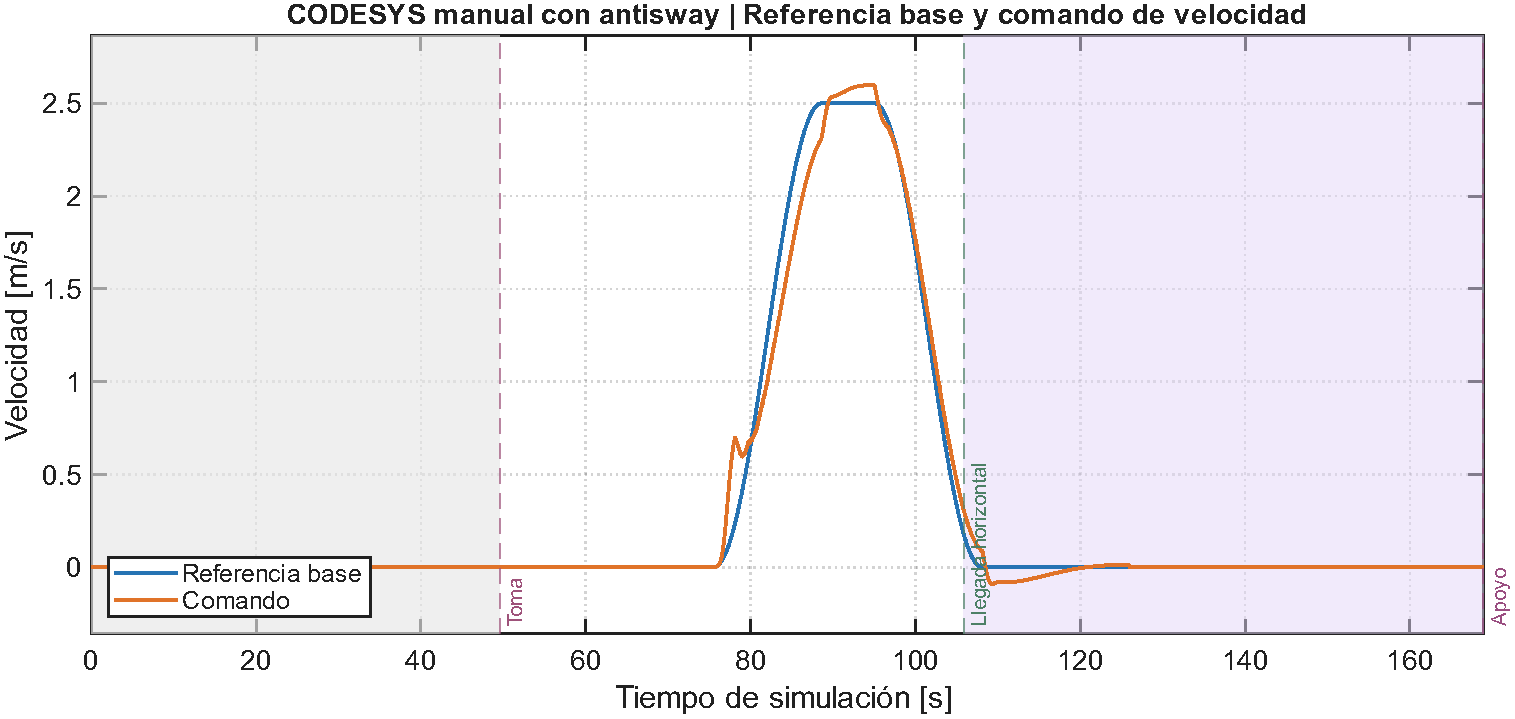
\includegraphics[width=0.98\textwidth]{graficas_individuales/manual_con_vcmd.pdf}
\caption{CODESYS manual con antisway: Referencia base y comando de velocidad; su diferencia corresponde a la contribución antisway efectiva en el sumador.}\label{fig:individual_manual_con_vcmd}
\end{figure}

\begin{figure}[!htbp]
\centering
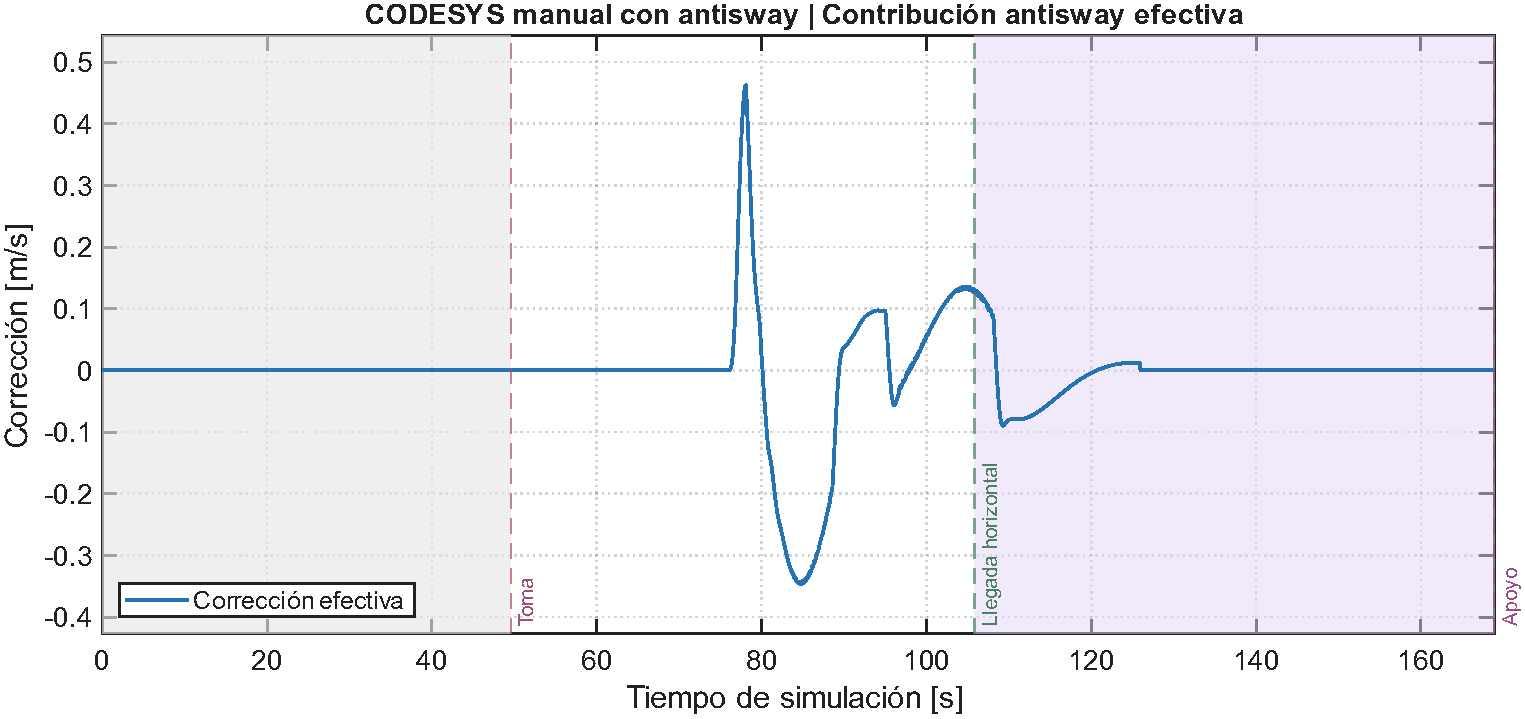
\includegraphics[width=0.98\textwidth]{graficas_individuales/manual_con_sw.pdf}
\caption{CODESYS manual con antisway: Contribución antisway efectivamente sumada al comando de velocidad.}\label{fig:individual_manual_con_sw}
\end{figure}

La masa física pasa del conjunto cargado al spreader vacío: $15\,000~\mathrm{kg}$ al final. El origen disminuye $2.59~\mathrm{m}$ y el destino aumenta $2.59~\mathrm{m}$. La posición final del carro fue $22.41138~\mathrm{m}$ y la altura $8.50636~\mathrm{m}$; el error horizontal al centro fue $0.04862~\mathrm{m}$. Estos datos confirman entrega física, además de la apertura de twistlocks. Los torques y la tensión muestran la respuesta al movimiento y al apoyo; la caída de masa distingue esta corrida de una llegada sin descarga. El registro físico y de control cubre la parada.

\begin{figure}[!htbp]
\centering
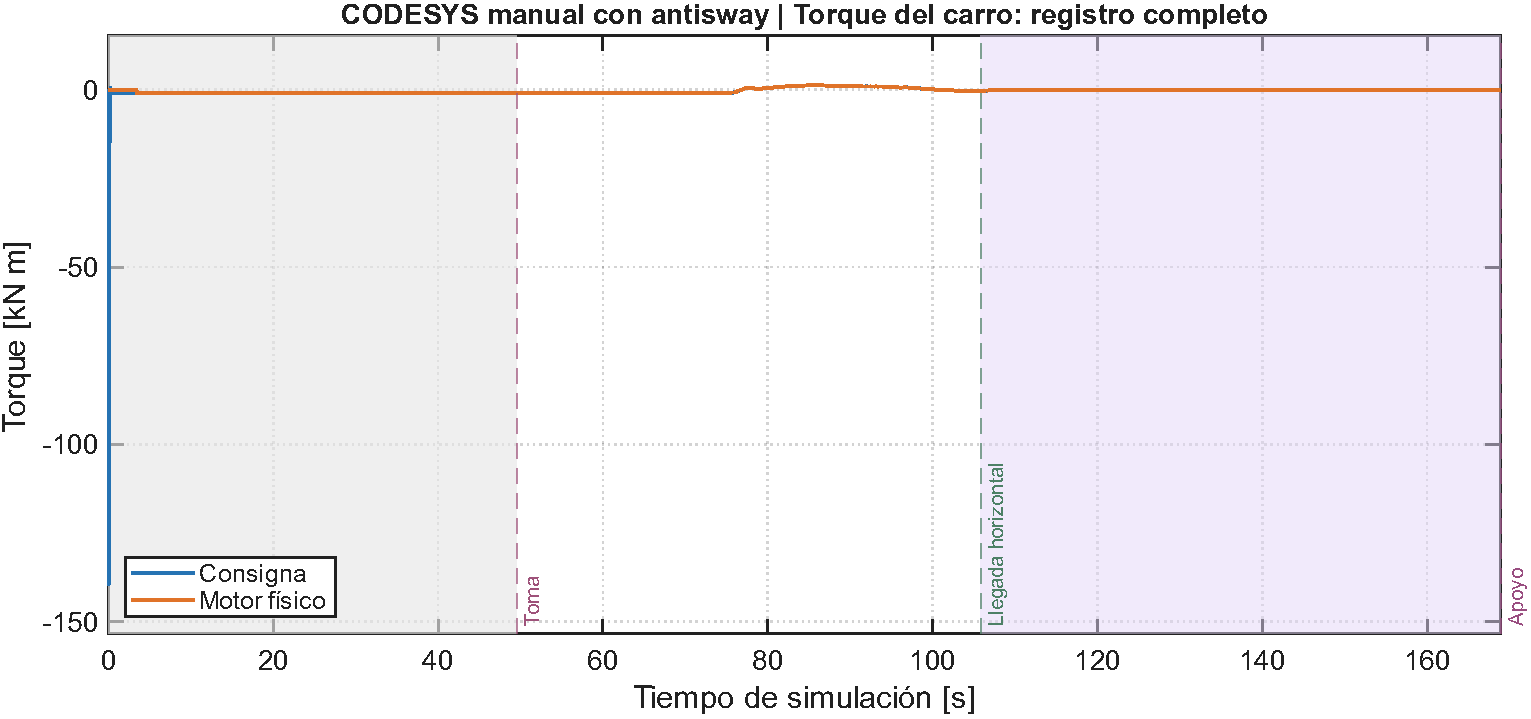
\includegraphics[width=0.98\textwidth]{graficas_individuales/manual_con_tx.pdf}
\caption{CODESYS manual con antisway: Consigna y torque físico del motor del carro en el intervalo representado, incluido el arranque.}\label{fig:individual_manual_con_tx}
\end{figure}

\begin{figure}[!htbp]
\centering
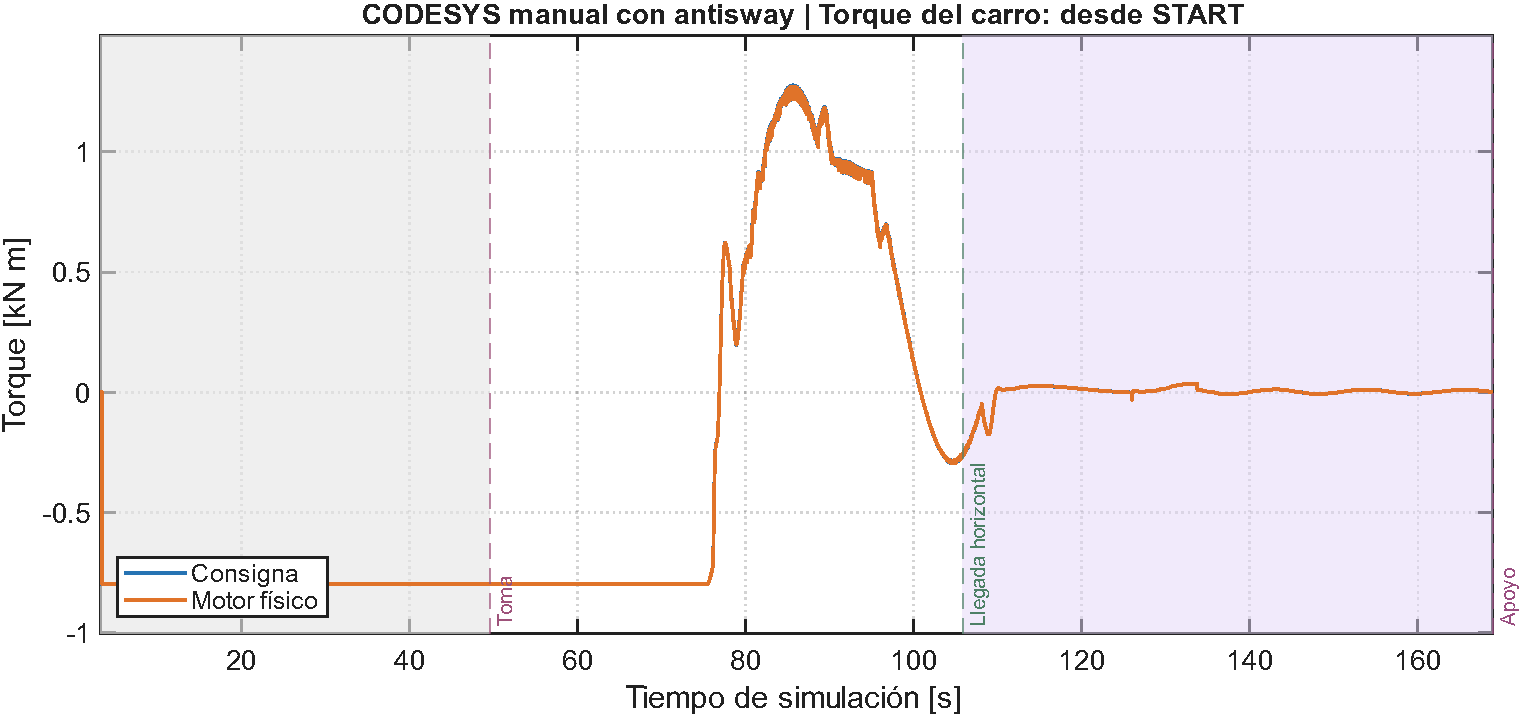
\includegraphics[width=0.98\textwidth]{graficas_individuales/manual_con_tx_zoom.pdf}
\caption{CODESYS manual con antisway: Consigna y torque físico del motor del carro desde START; la escala completa del arranque se conserva en una figura independiente.}\label{fig:individual_manual_con_tx_zoom}
\end{figure}

\begin{figure}[!htbp]
\centering
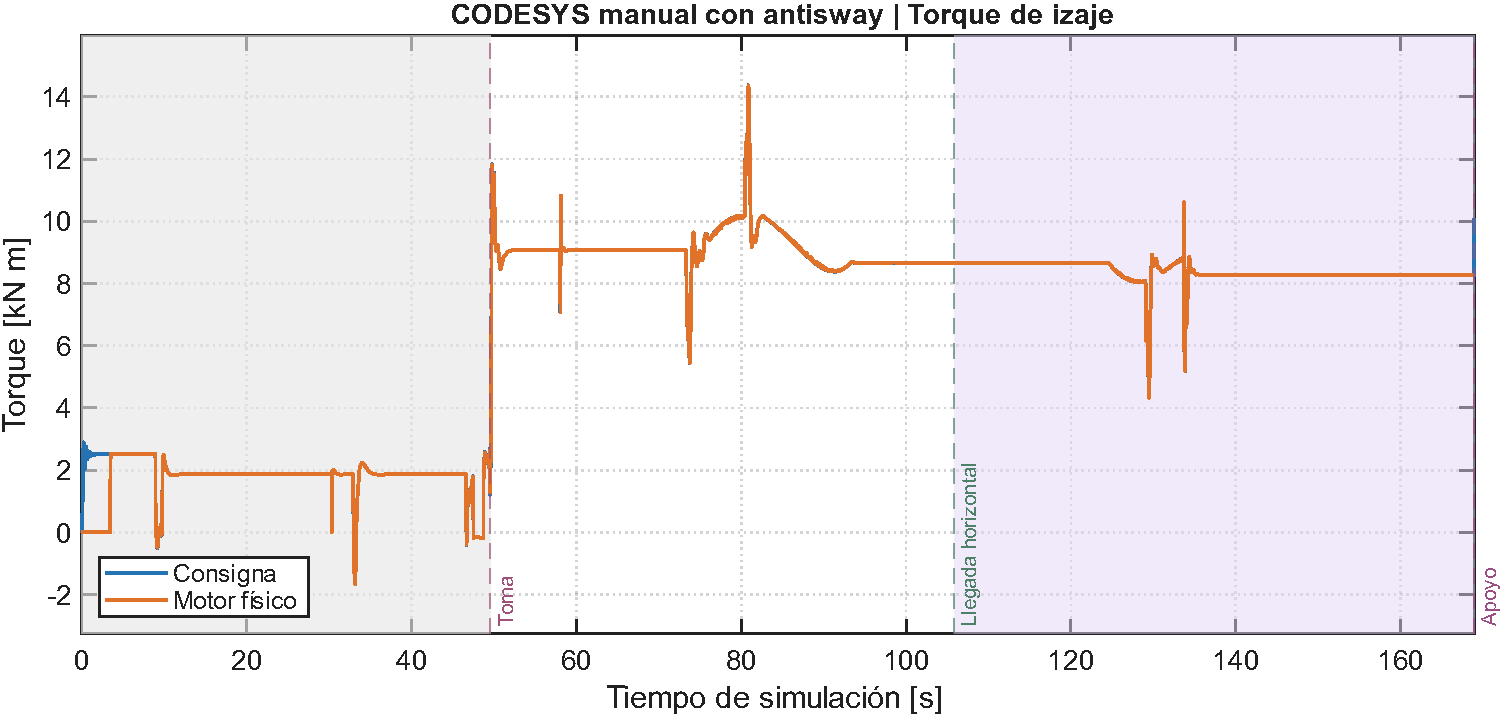
\includegraphics[width=0.98\textwidth]{graficas_individuales/manual_con_ty.pdf}
\caption{CODESYS manual con antisway: Consigna del controlador y torque físico del motor de izaje.}\label{fig:individual_manual_con_ty}
\end{figure}

\begin{figure}[!htbp]
\centering
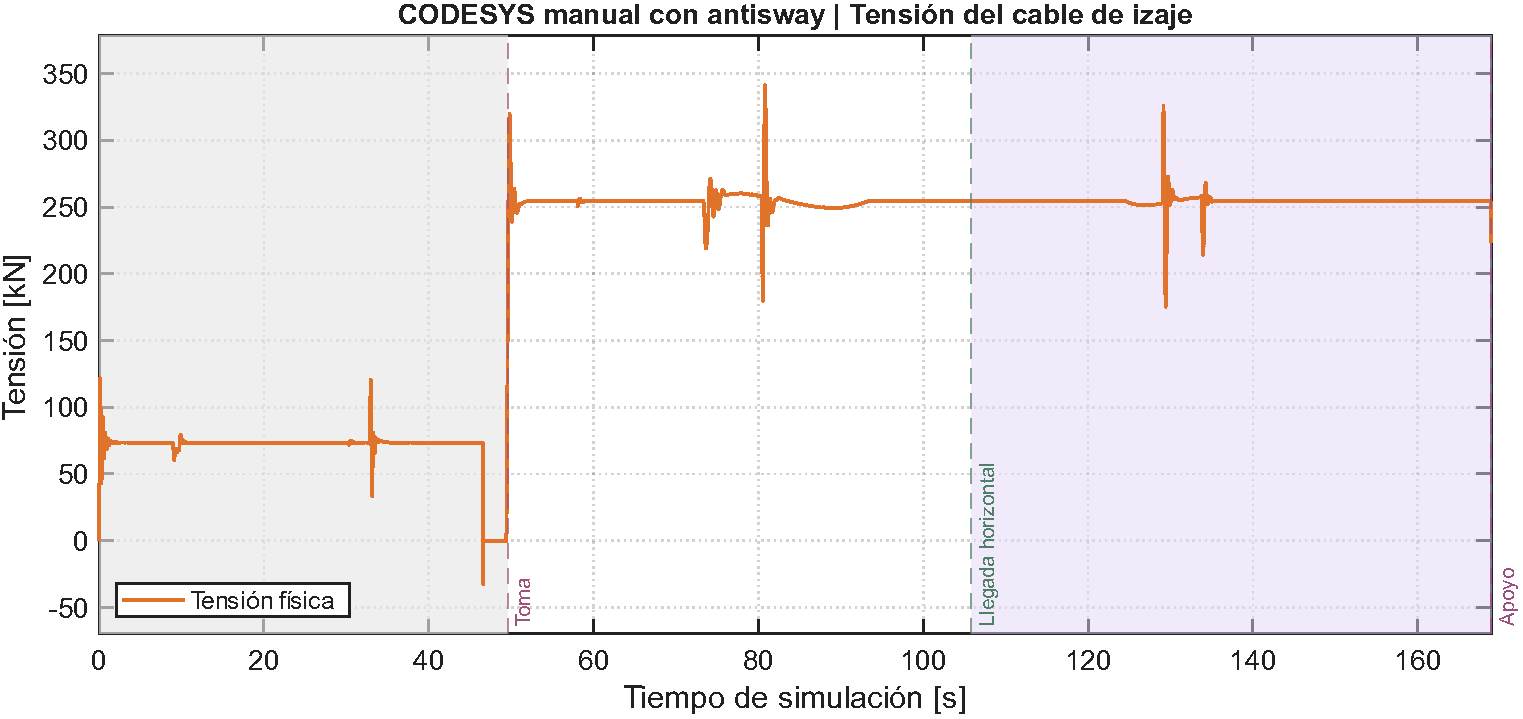
\includegraphics[width=0.98\textwidth]{graficas_individuales/manual_con_tension.pdf}
\caption{CODESYS manual con antisway: Tensión física del cable de izaje.}\label{fig:individual_manual_con_tension}
\end{figure}

\begin{figure}[!htbp]
\centering
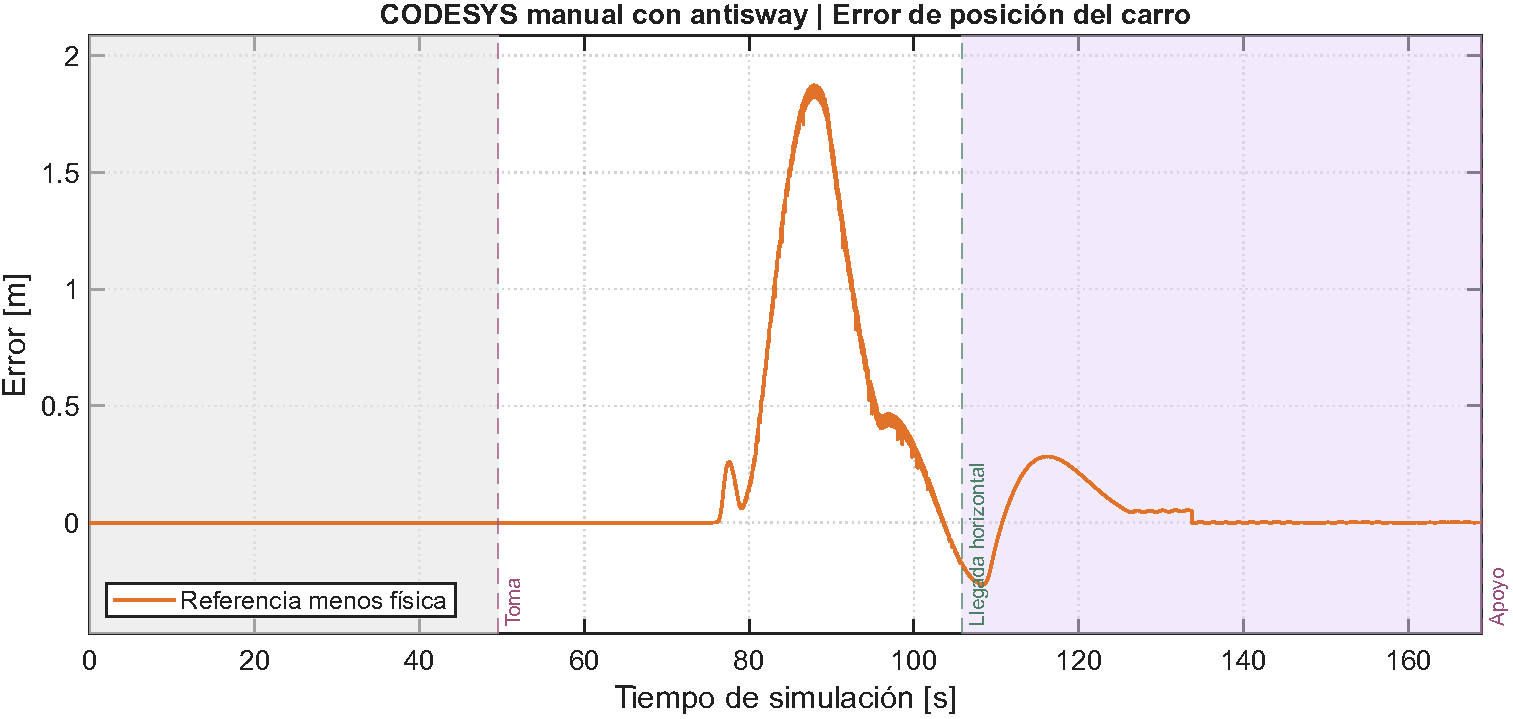
\includegraphics[width=0.98\textwidth]{graficas_individuales/manual_con_ex.pdf}
\caption{CODESYS manual con antisway: Error horizontal, calculado como referencia menos posición física.}\label{fig:individual_manual_con_ex}
\end{figure}

\begin{figure}[!htbp]
\centering
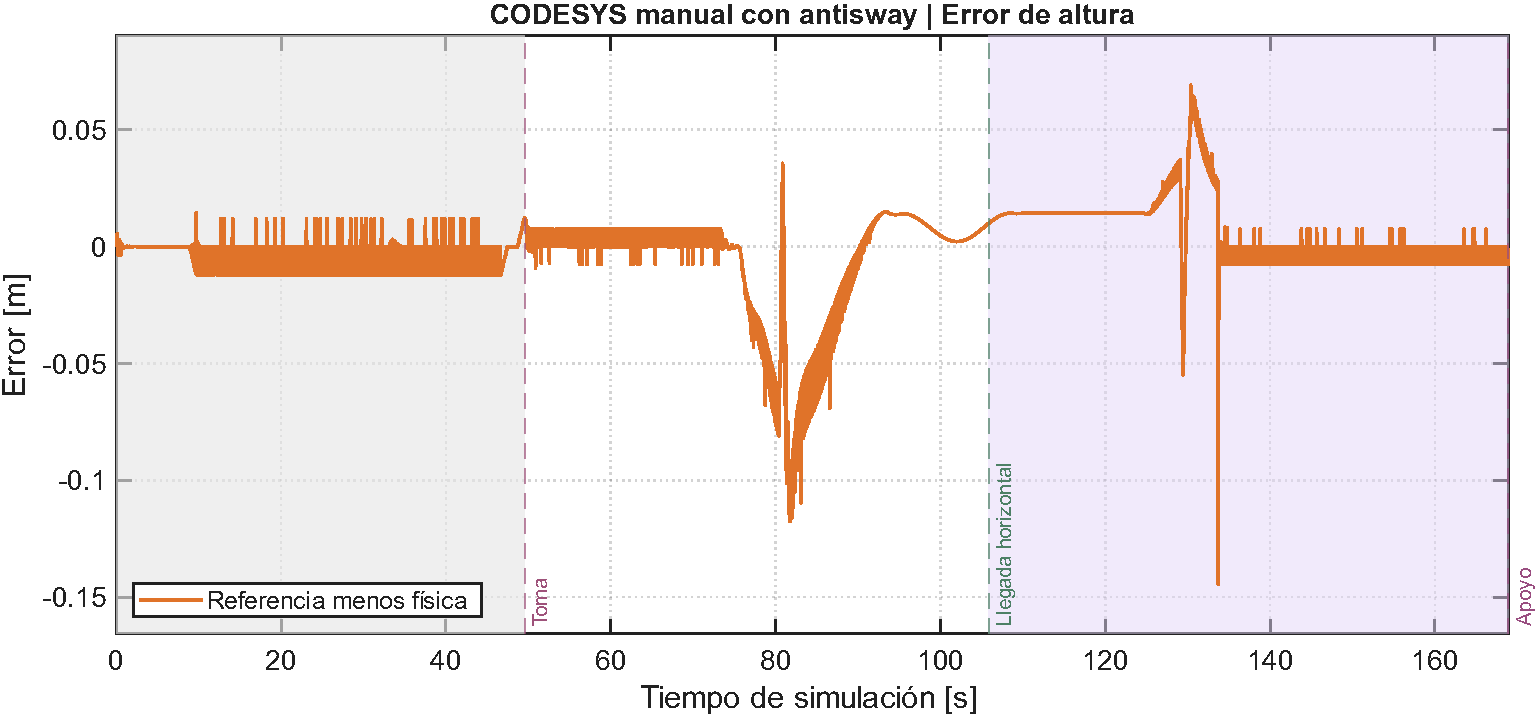
\includegraphics[width=0.98\textwidth]{graficas_individuales/manual_con_ey.pdf}
\caption{CODESYS manual con antisway: Error de altura, calculado como referencia menos altura física.}\label{fig:individual_manual_con_ey}
\end{figure}

\begin{figure}[!htbp]
\centering
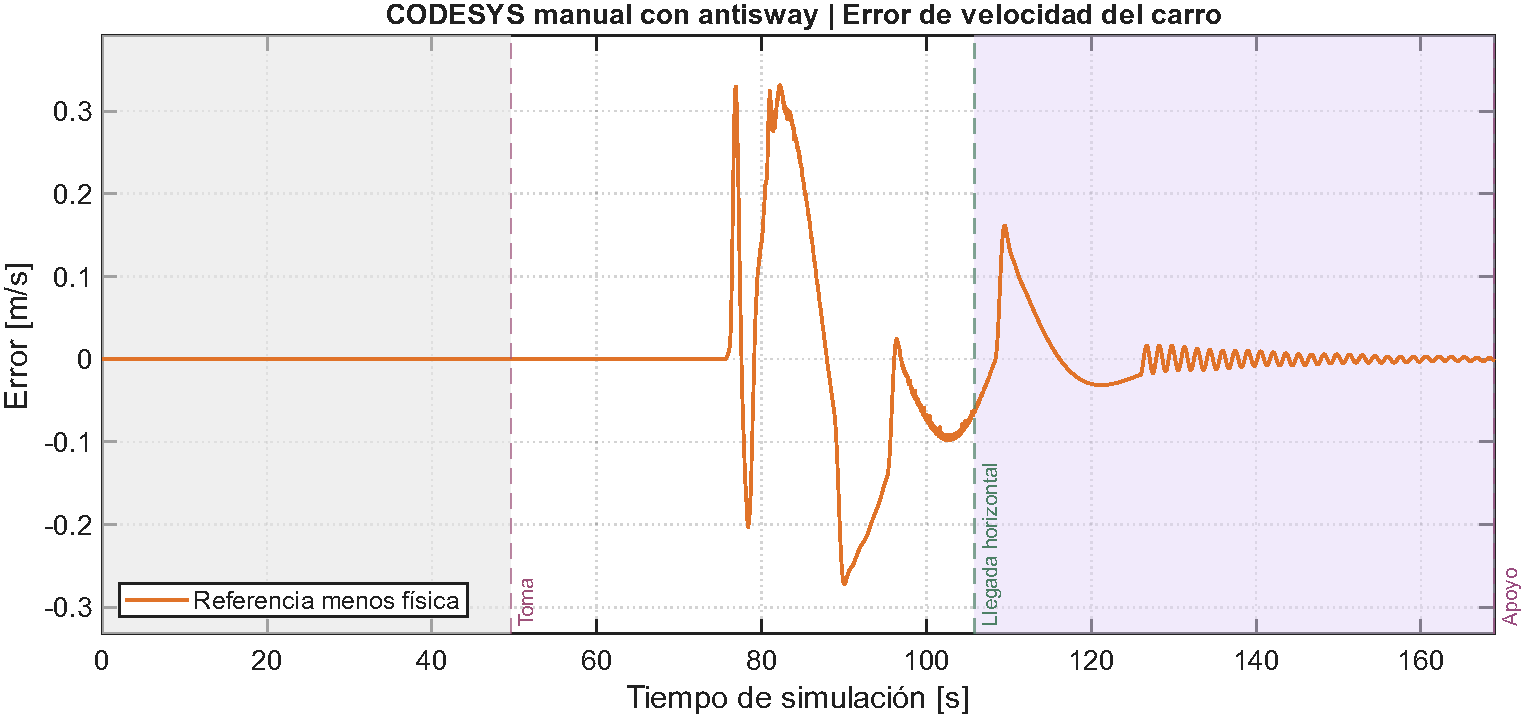
\includegraphics[width=0.98\textwidth]{graficas_individuales/manual_con_evx.pdf}
\caption{CODESYS manual con antisway: Error de velocidad del carro, calculado como referencia menos velocidad física.}\label{fig:individual_manual_con_evx}
\end{figure}

\begin{figure}[!htbp]
\centering
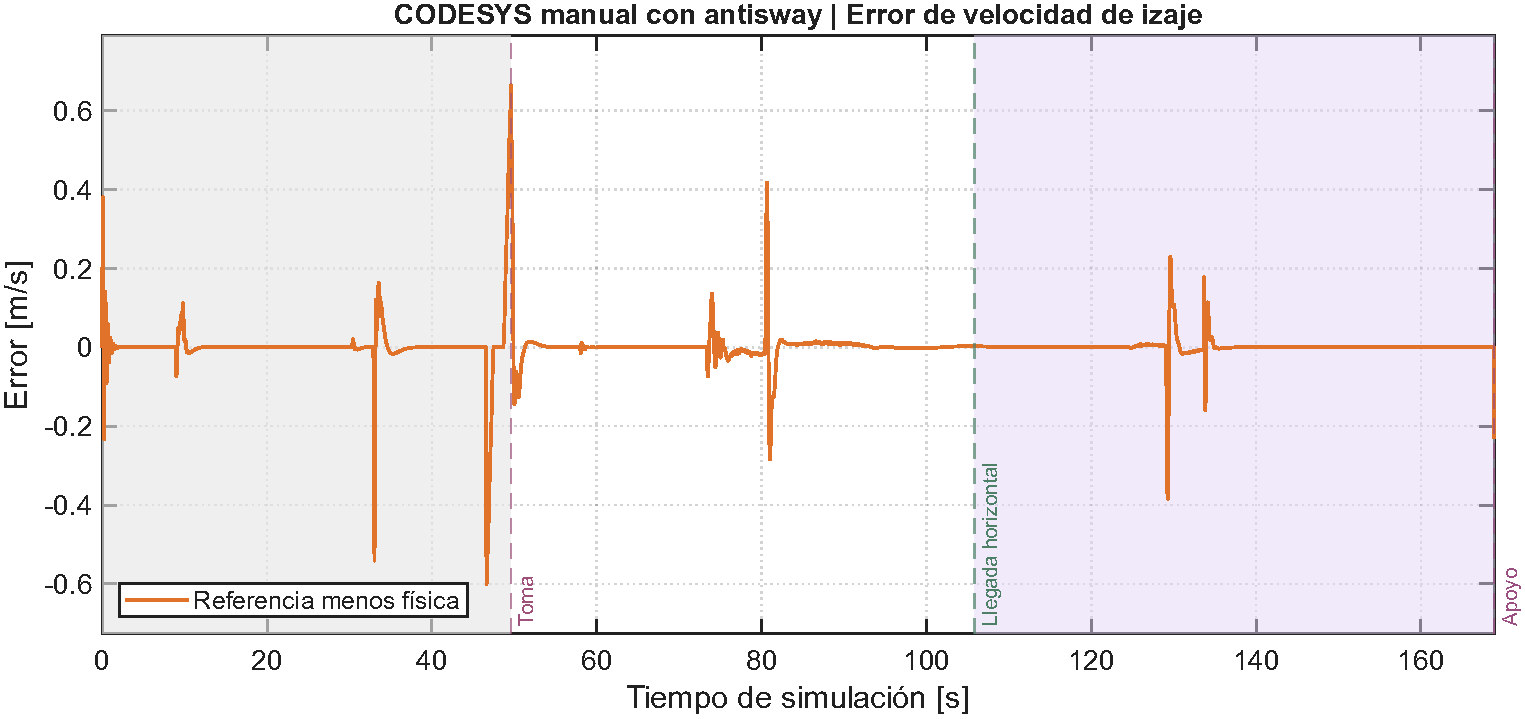
\includegraphics[width=0.98\textwidth]{graficas_individuales/manual_con_evy.pdf}
\caption{CODESYS manual con antisway: Error de velocidad de izaje, calculado como referencia menos velocidad física.}\label{fig:individual_manual_con_evy}
\end{figure}

\begin{figure}[!htbp]
\centering
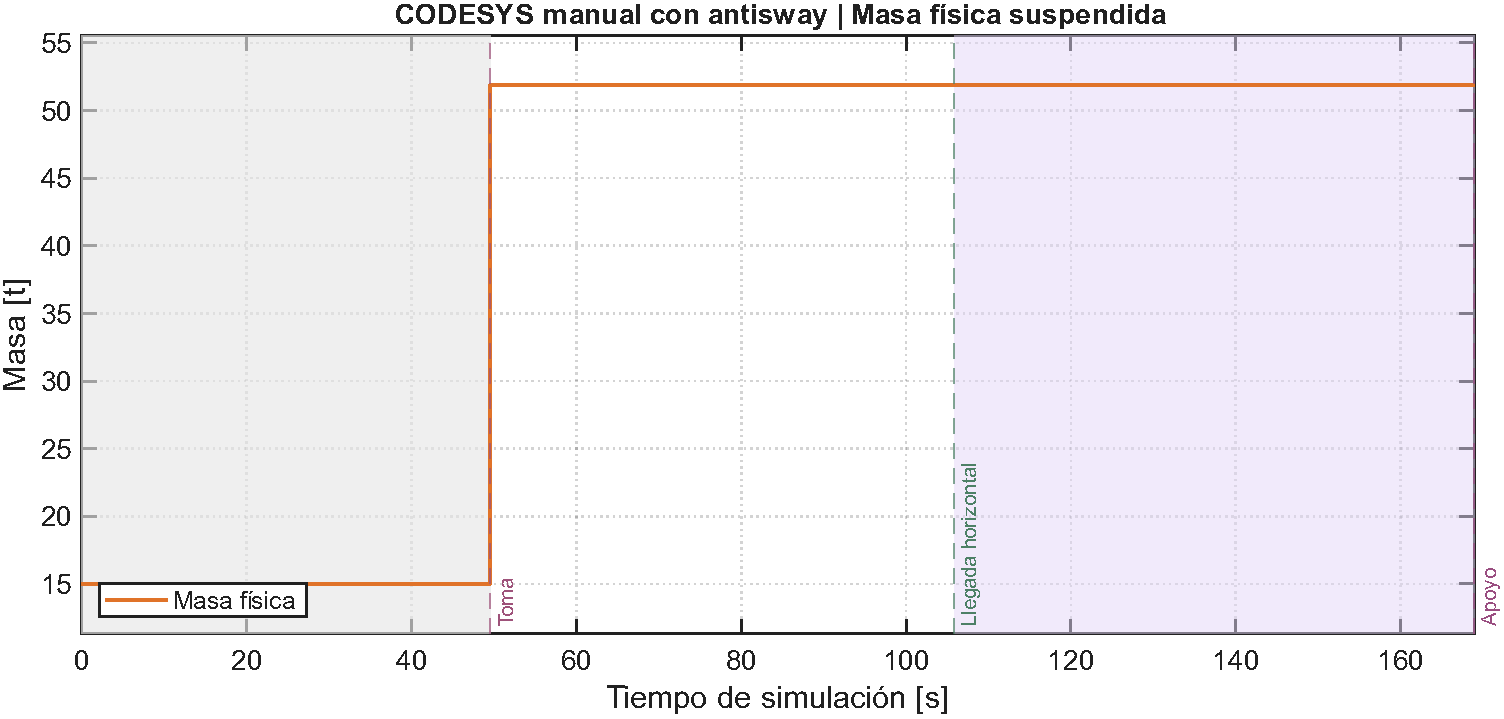
\includegraphics[width=0.98\textwidth]{graficas_individuales/manual_con_masa.pdf}
\caption{CODESYS manual con antisway: Masa física suspendida: 51,863 t representa conjunto cargado y 15 t corresponde al spreader vacío.}\label{fig:individual_manual_con_masa}
\end{figure}

\begin{figure}[!htbp]
\centering
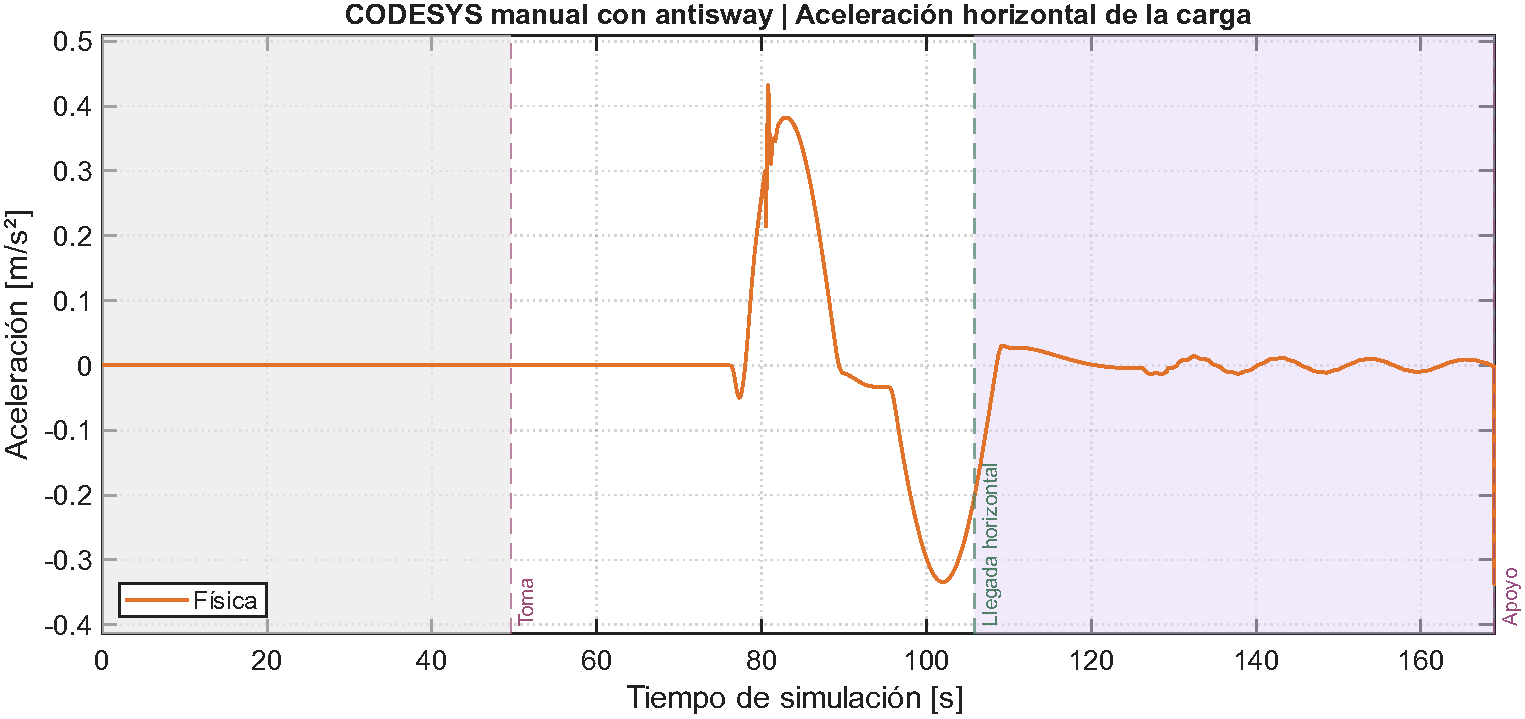
\includegraphics[width=0.98\textwidth]{graficas_individuales/manual_con_ax_carga.pdf}
\caption{CODESYS manual con antisway: Aceleración horizontal física de la carga; se conservan las oscilaciones registradas.}\label{fig:individual_manual_con_ax_carga}
\end{figure}

\clearpage
\section{Pruebas de medio ciclo con CODESYS automático}
\label{sec:ensayo_codesys_st}
\subsection{Alcance de la implementación ensayada}
Se repitió el procedimiento con supervisor y seguridad en texto estructurado generado mediante Simulink PLC Coder, con adaptadores para intercambio OPC UA, precarga del perfil y sincronización por trama. La planta, el controlador regulatorio y la HMI fueron los mismos del ensayo manual. El código generado ejecuta las máquinas de estados al recibir una nueva trama de tiempo simulado; los interbloqueos finales y la vigilancia de enlace conservan el reloj real. Esta adaptación del banco no modifica los criterios de estabilización ni fuerza la entrega física.

\subsection{CODESYS automático sin antisway: parada al límite de tres minutos}
START se solicitó a $3.24~\mathrm{s}$ y el modo manual se observó a $3.76~\mathrm{s}$. El cierre se solicitó a $46.64~\mathrm{s}$, la masa cargada se confirmó a $49.52~\mathrm{s}$ y el despegue físico a $50.00~\mathrm{s}$. Automático se solicitó a $75.28~\mathrm{s}$ y se observó a $75.36~\mathrm{s}$; la llegada horizontal fue a $105.60~\mathrm{s}$. La parada programada ocurrió exactamente a $180.00~\mathrm{s}$ sin entrega.

El carro alcanzó $22.39992~\mathrm{m}$, pero la carga permaneció a $24.07414~\mathrm{m}$ con masa $51\,863~\mathrm{kg}$. Las curvas muestran llegada horizontal y oscilación residual mientras la altura permanece en la zona de cruce. No se produjo transferencia a manual ni apoyo final. El resultado es válido para diagnóstico del control sin antisway y no aprobado como medio ciclo completo.

\begin{figure}[!htbp]
\centering
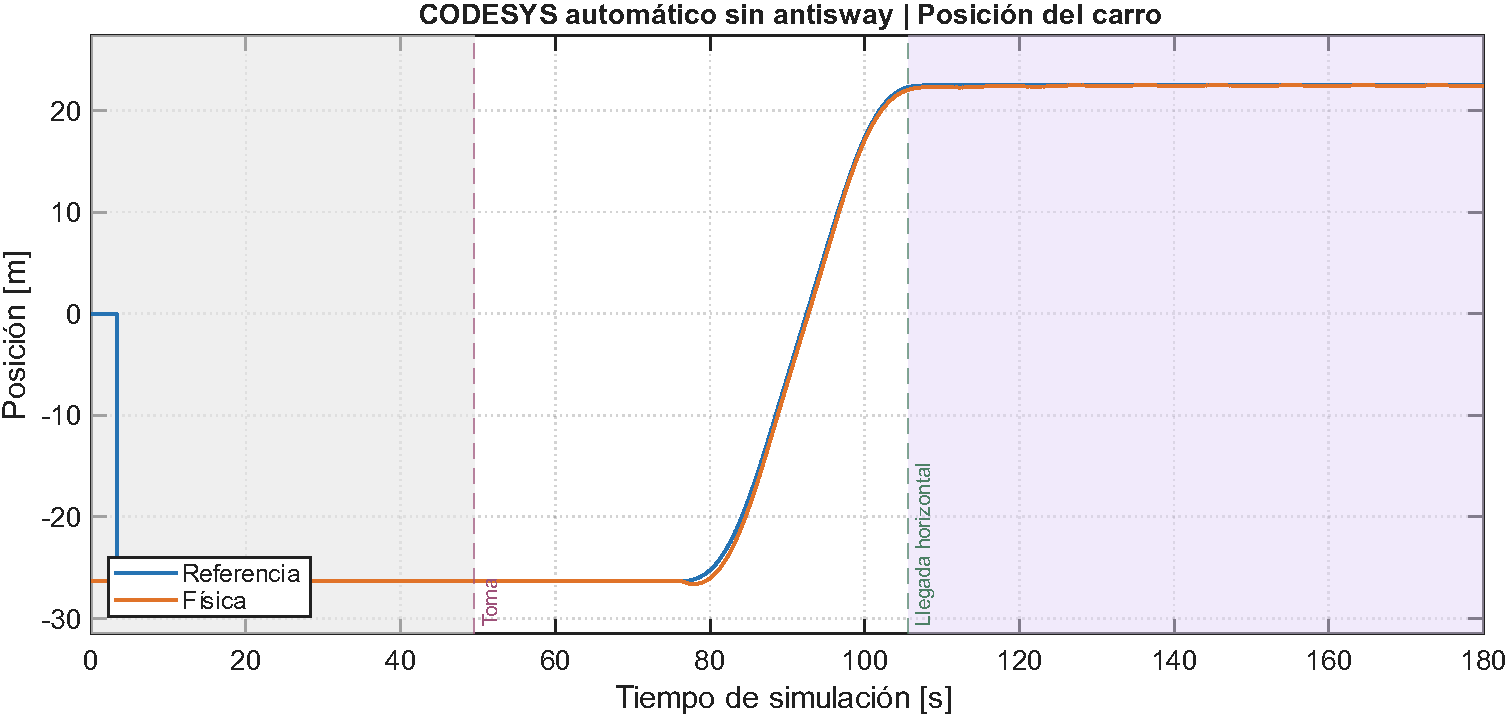
\includegraphics[width=0.98\textwidth]{graficas_individuales/automatico_sin_x.pdf}
\caption{CODESYS automático sin antisway: Posición del carro: referencia y evolución física.}\label{fig:individual_automatico_sin_x}
\end{figure}

\begin{figure}[!htbp]
\centering
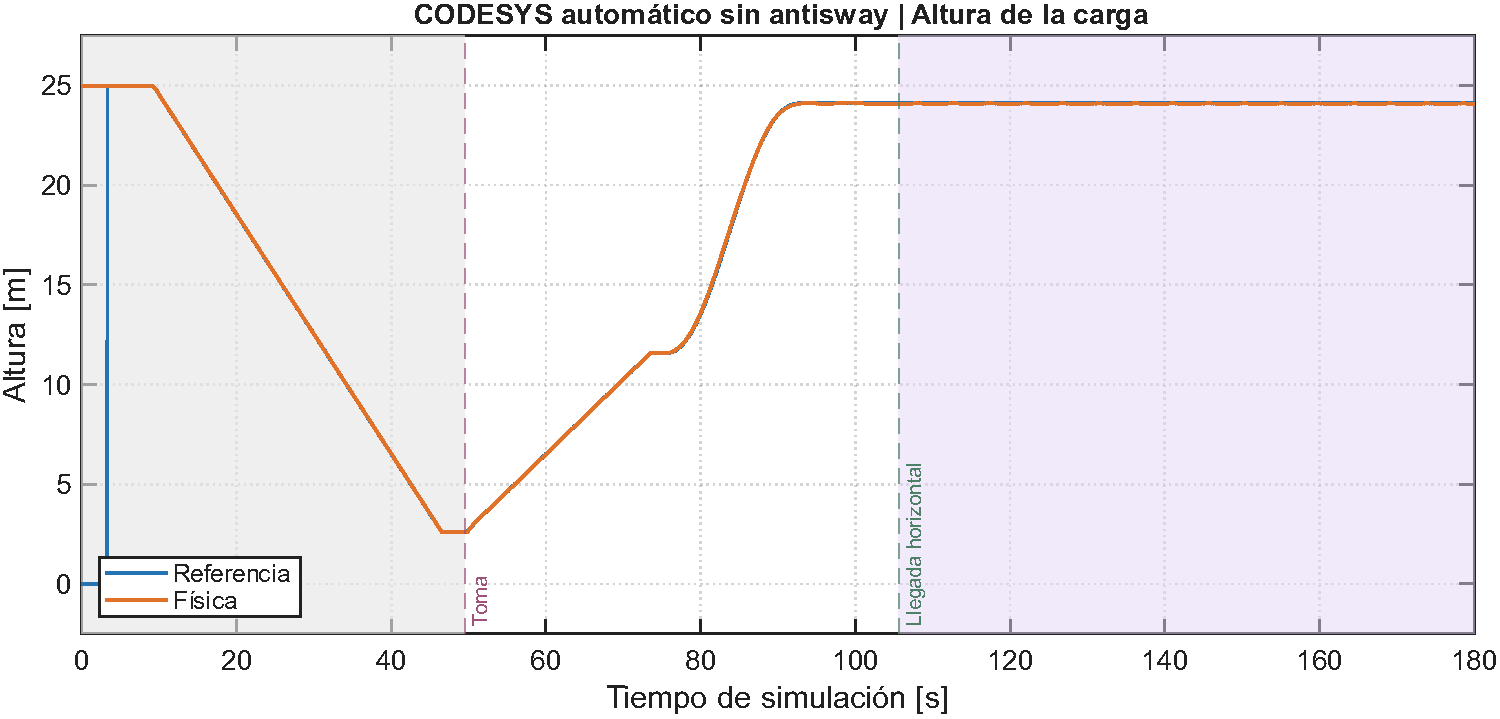
\includegraphics[width=0.98\textwidth]{graficas_individuales/automatico_sin_y.pdf}
\caption{CODESYS automático sin antisway: Altura de la carga: referencia y evolución física.}\label{fig:individual_automatico_sin_y}
\end{figure}

\begin{figure}[!htbp]
\centering
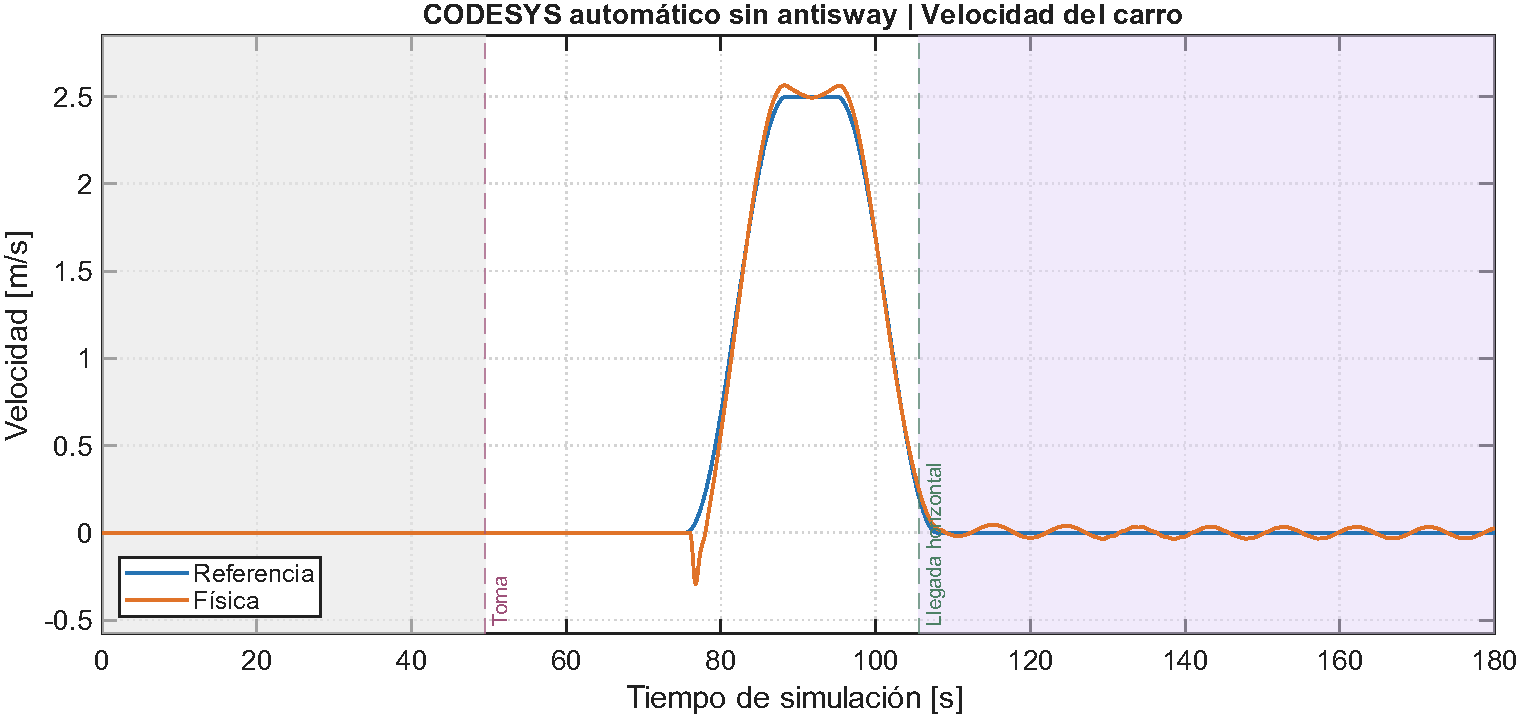
\includegraphics[width=0.98\textwidth]{graficas_individuales/automatico_sin_vx.pdf}
\caption{CODESYS automático sin antisway: Velocidad del carro: referencia y señal física.}\label{fig:individual_automatico_sin_vx}
\end{figure}

\begin{figure}[!htbp]
\centering
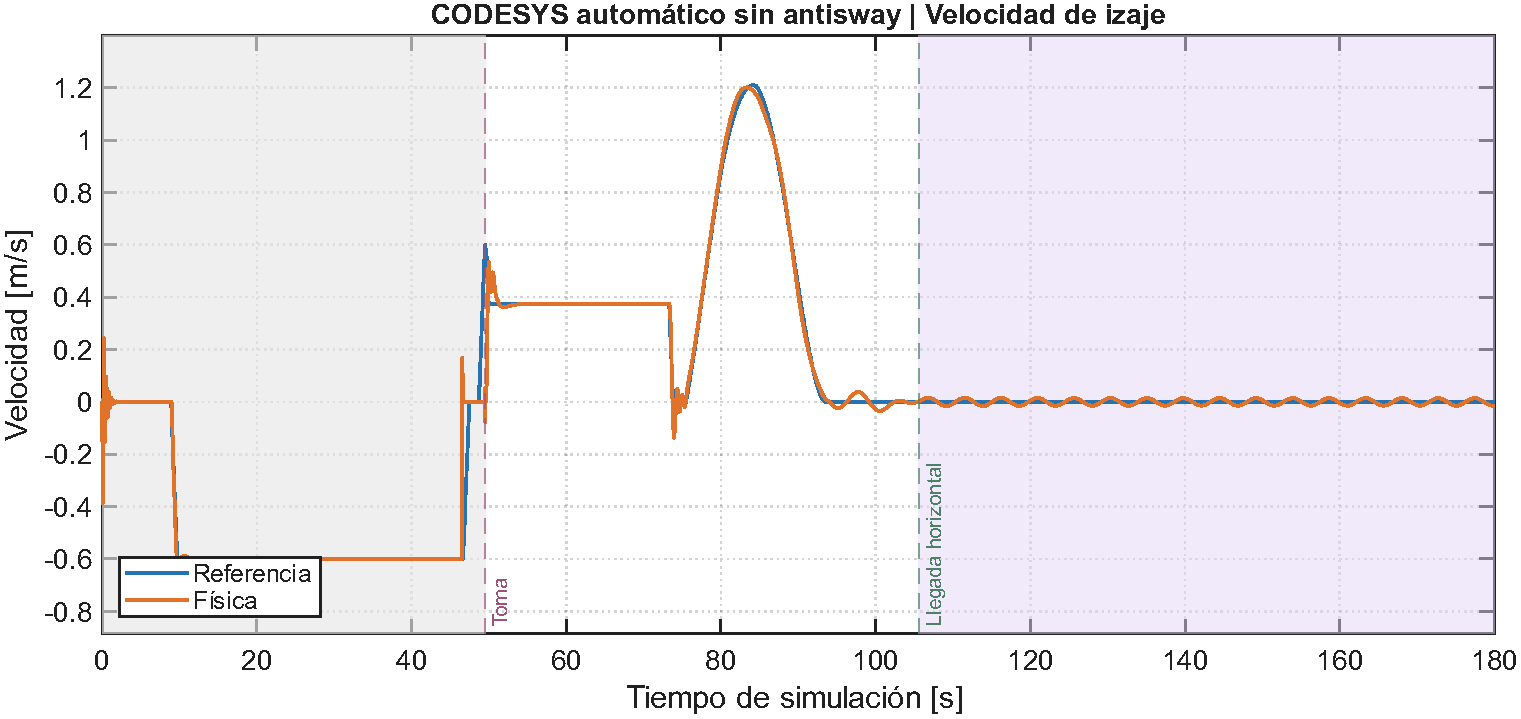
\includegraphics[width=0.98\textwidth]{graficas_individuales/automatico_sin_vy.pdf}
\caption{CODESYS automático sin antisway: Velocidad de izaje: referencia y señal física.}\label{fig:individual_automatico_sin_vy}
\end{figure}

\begin{figure}[!htbp]
\centering
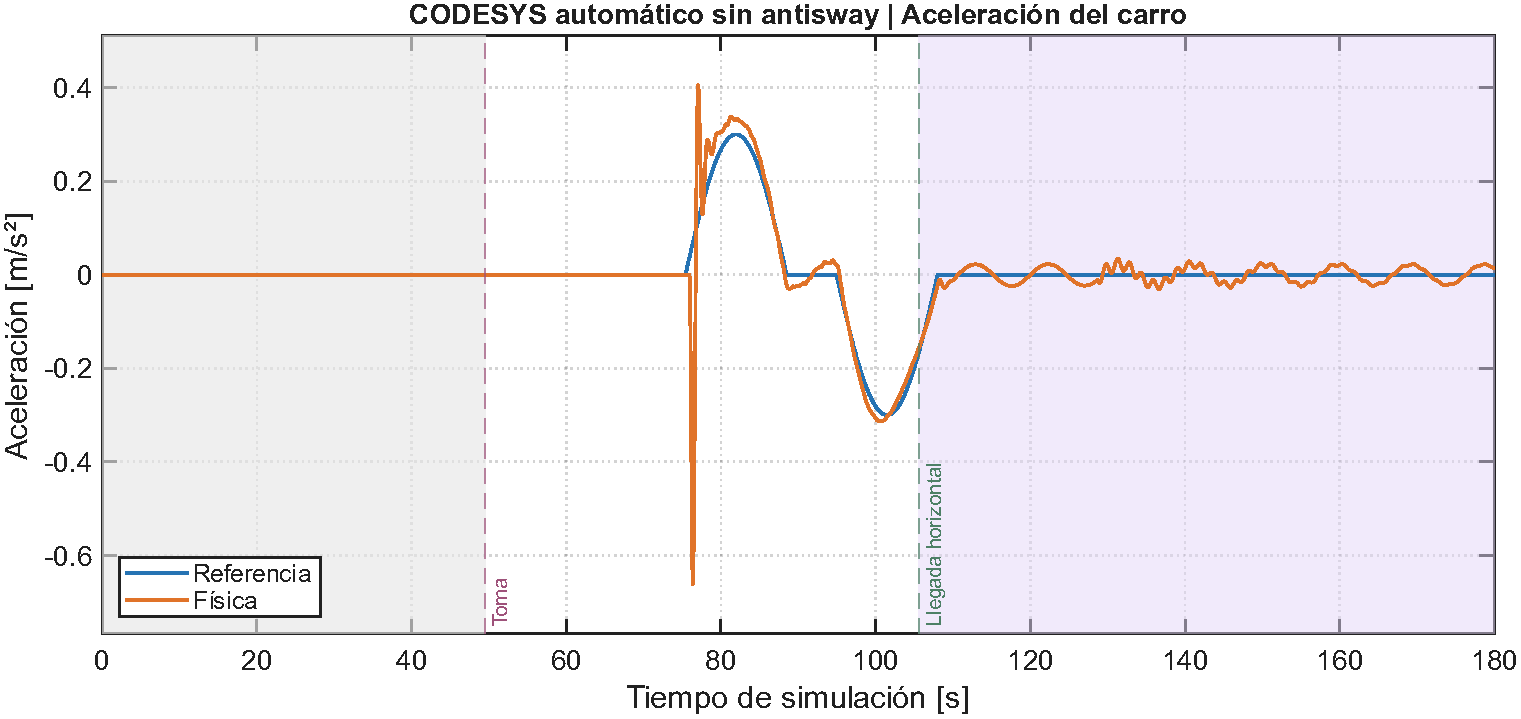
\includegraphics[width=0.98\textwidth]{graficas_individuales/automatico_sin_ax.pdf}
\caption{CODESYS automático sin antisway: Aceleración del carro: referencia y señal física.}\label{fig:individual_automatico_sin_ax}
\end{figure}

\begin{figure}[!htbp]
\centering
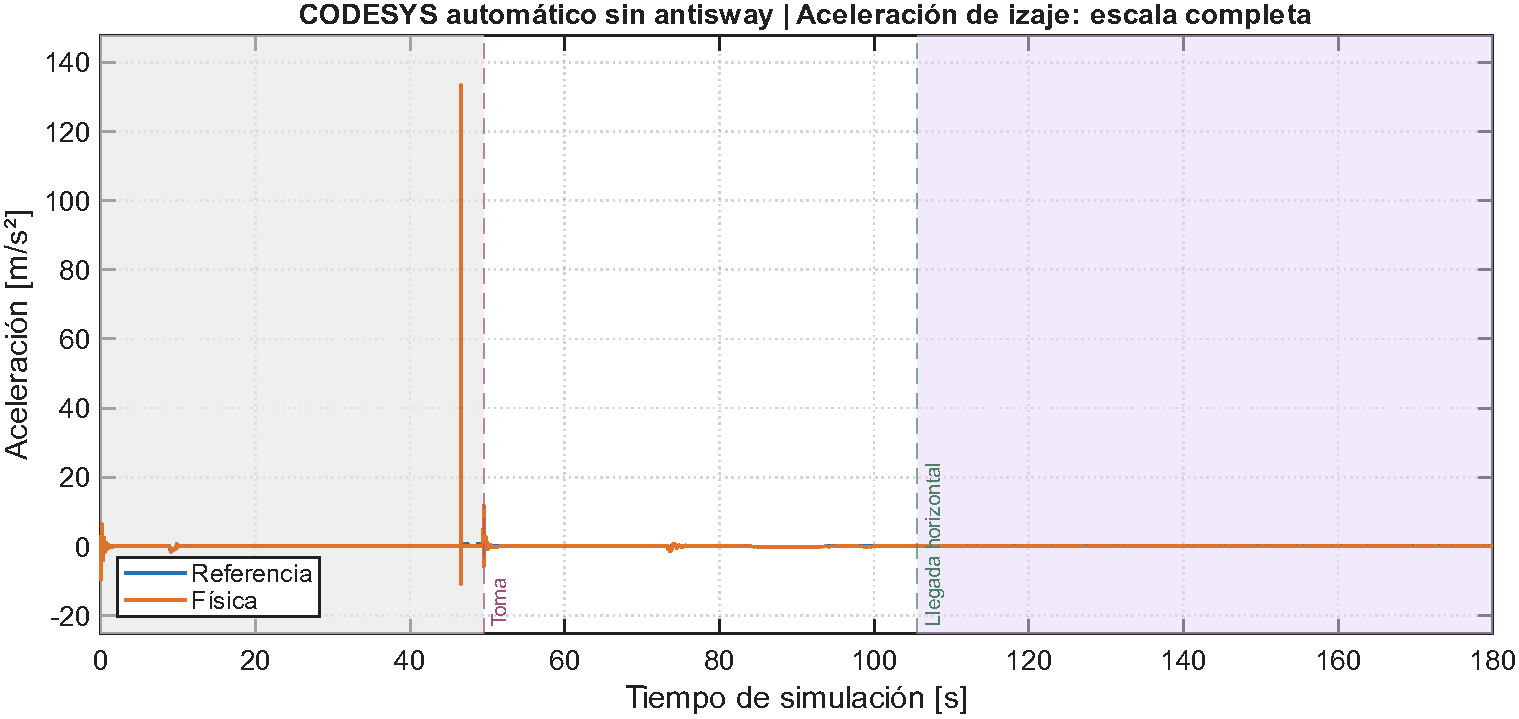
\includegraphics[width=0.98\textwidth]{graficas_individuales/automatico_sin_ay.pdf}
\caption{CODESYS automático sin antisway: Aceleración de izaje en escala completa; se conservan los picos de contacto y arranque.}\label{fig:individual_automatico_sin_ay}
\end{figure}

\begin{figure}[!htbp]
\centering
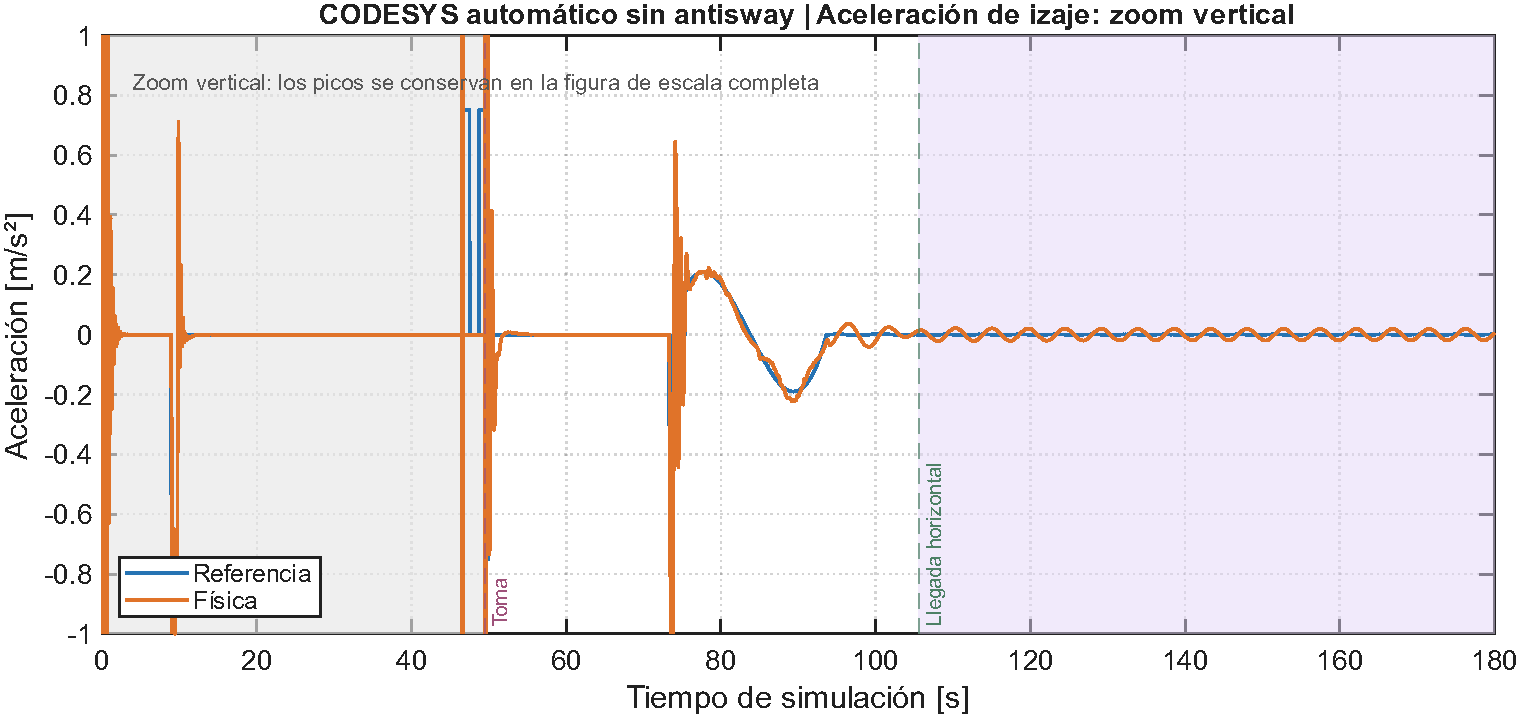
\includegraphics[width=0.98\textwidth]{graficas_individuales/automatico_sin_ay_zoom.pdf}
\caption{CODESYS automático sin antisway: Aceleración de izaje con zoom vertical entre $-1$ y $+1~\mathrm{m/s^2}$ para observar su evolución temporal. Los picos que exceden este intervalo permanecen visibles en la figura de escala completa; no se filtraron las señales.}\label{fig:individual_automatico_sin_ay_zoom}
\end{figure}

\begin{figure}[!htbp]
\centering
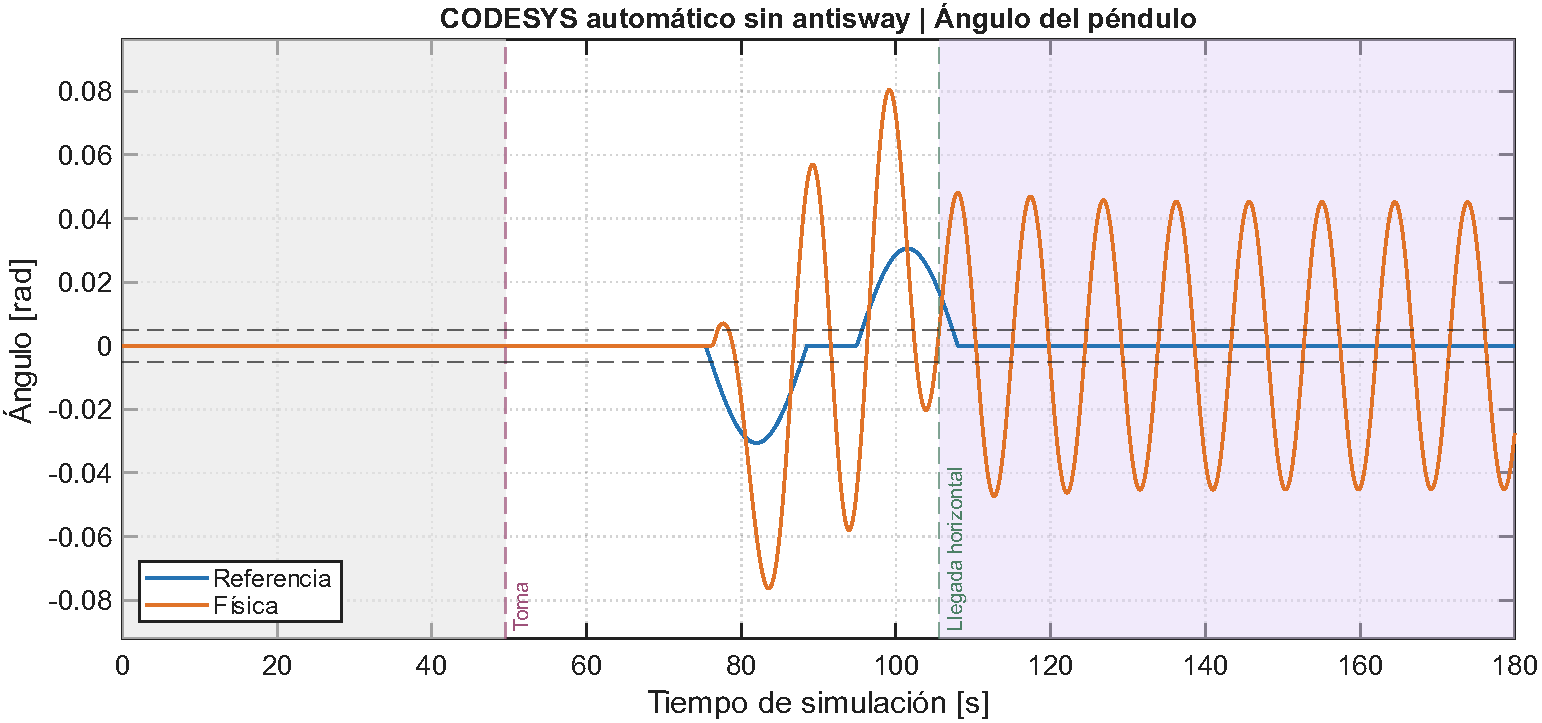
\includegraphics[width=0.98\textwidth]{graficas_individuales/automatico_sin_theta.pdf}
\caption{CODESYS automático sin antisway: Ángulo físico y de referencia del péndulo. Las líneas horizontales señalan los umbrales angulares del descenso.}\label{fig:individual_automatico_sin_theta}
\end{figure}

\begin{figure}[!htbp]
\centering
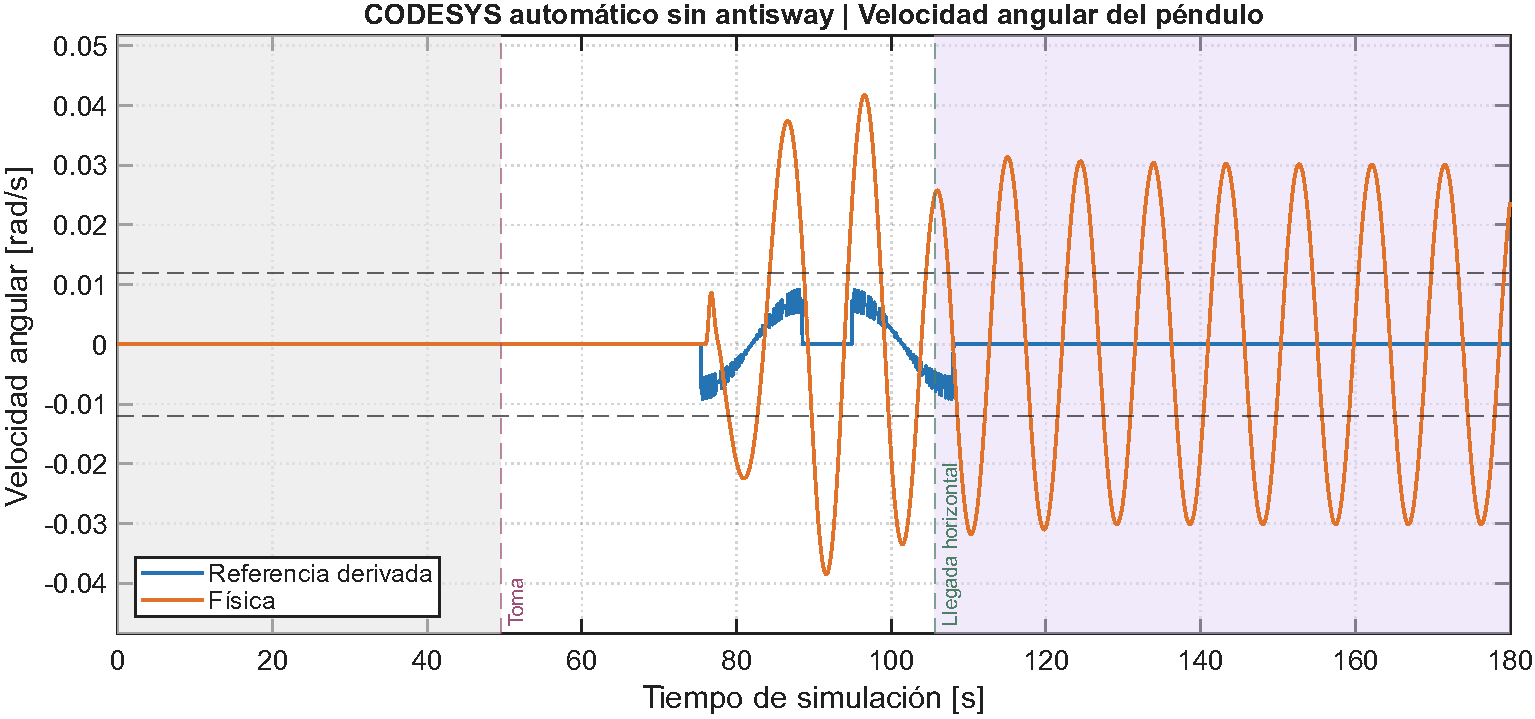
\includegraphics[width=0.98\textwidth]{graficas_individuales/automatico_sin_omega.pdf}
\caption{CODESYS automático sin antisway: Velocidad angular física y referencia derivada numéricamente; se distinguen ambas fuentes. Las líneas horizontales indican los umbrales del descenso.}\label{fig:individual_automatico_sin_omega}
\end{figure}

\begin{figure}[!htbp]
\centering
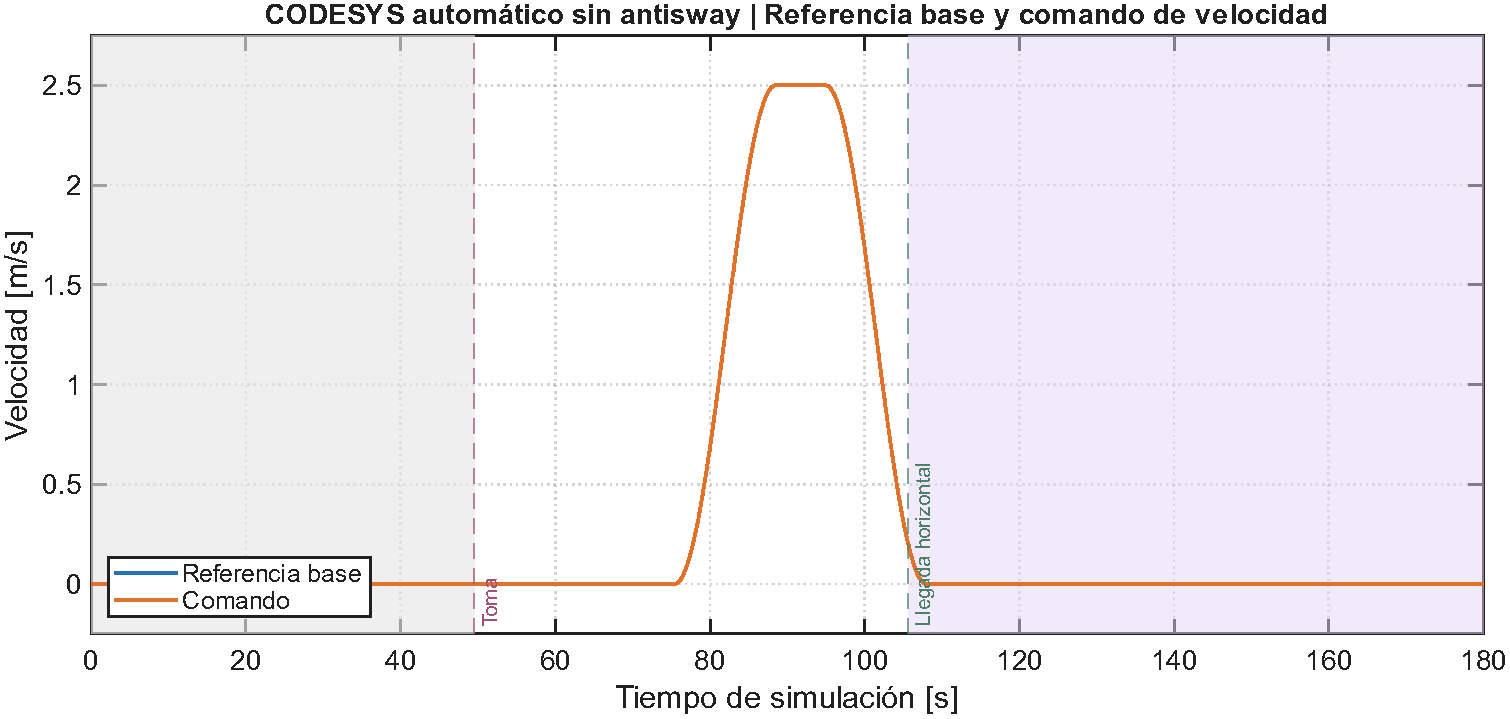
\includegraphics[width=0.98\textwidth]{graficas_individuales/automatico_sin_vcmd.pdf}
\caption{CODESYS automático sin antisway: Referencia base y comando de velocidad; su diferencia corresponde a la contribución antisway efectiva en el sumador.}\label{fig:individual_automatico_sin_vcmd}
\end{figure}

\begin{figure}[!htbp]
\centering
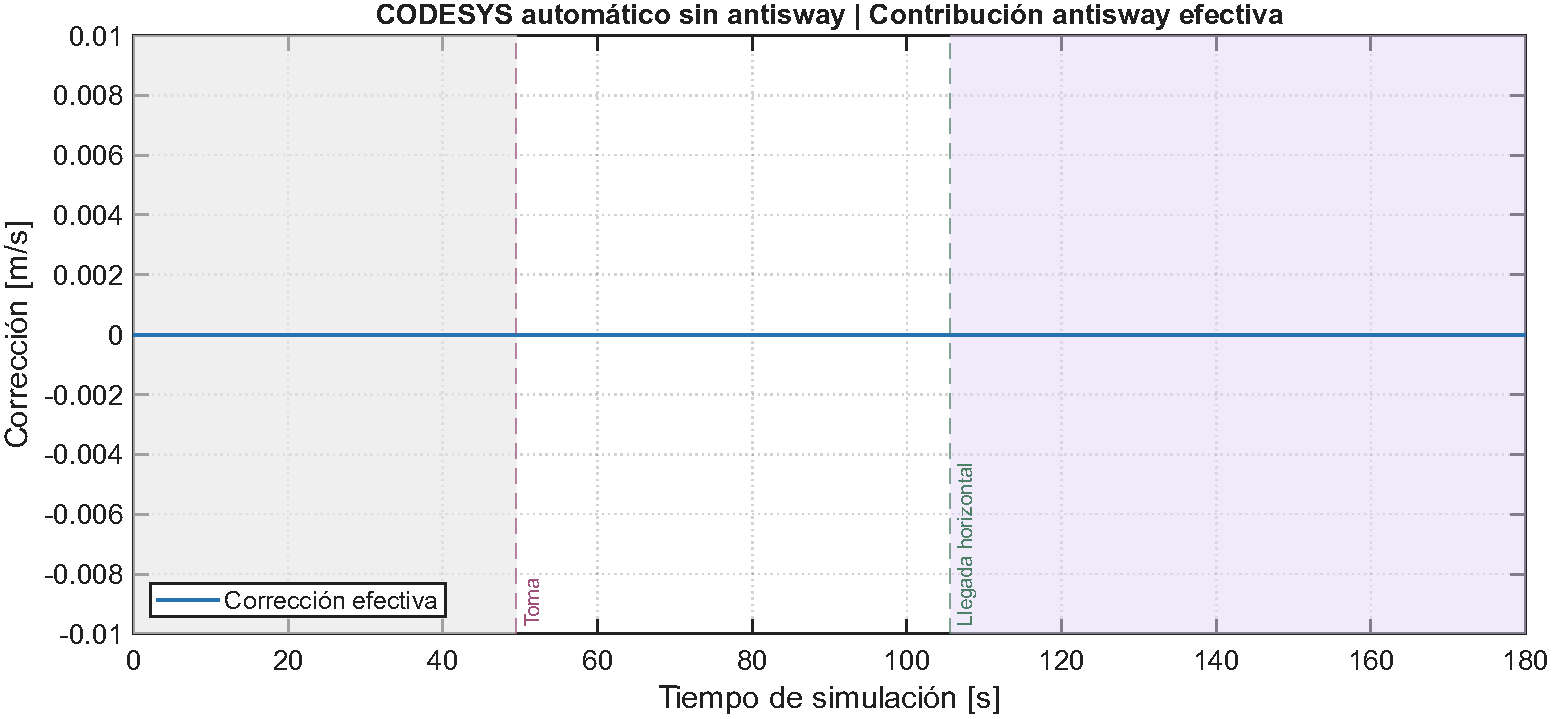
\includegraphics[width=0.98\textwidth]{graficas_individuales/automatico_sin_sw.pdf}
\caption{CODESYS automático sin antisway: Contribución antisway efectivamente sumada al comando de velocidad.}\label{fig:individual_automatico_sin_sw}
\end{figure}

La verificación nativa confirmó corrección efectiva cero y comando igual a referencia en las $180\,001$ muestras del controlador. El registro completo permite observar los torques, aceleraciones y tensión hasta la parada, sin el faltante de la variante manual sin antisway. La masa física no cae a la del spreader y el perfil del destino no aumenta. La indicación de antisway habilitado en la HMI corresponde a permiso de ejecución; la ganancia experimental cero impide su contribución al comando.

\begin{figure}[!htbp]
\centering
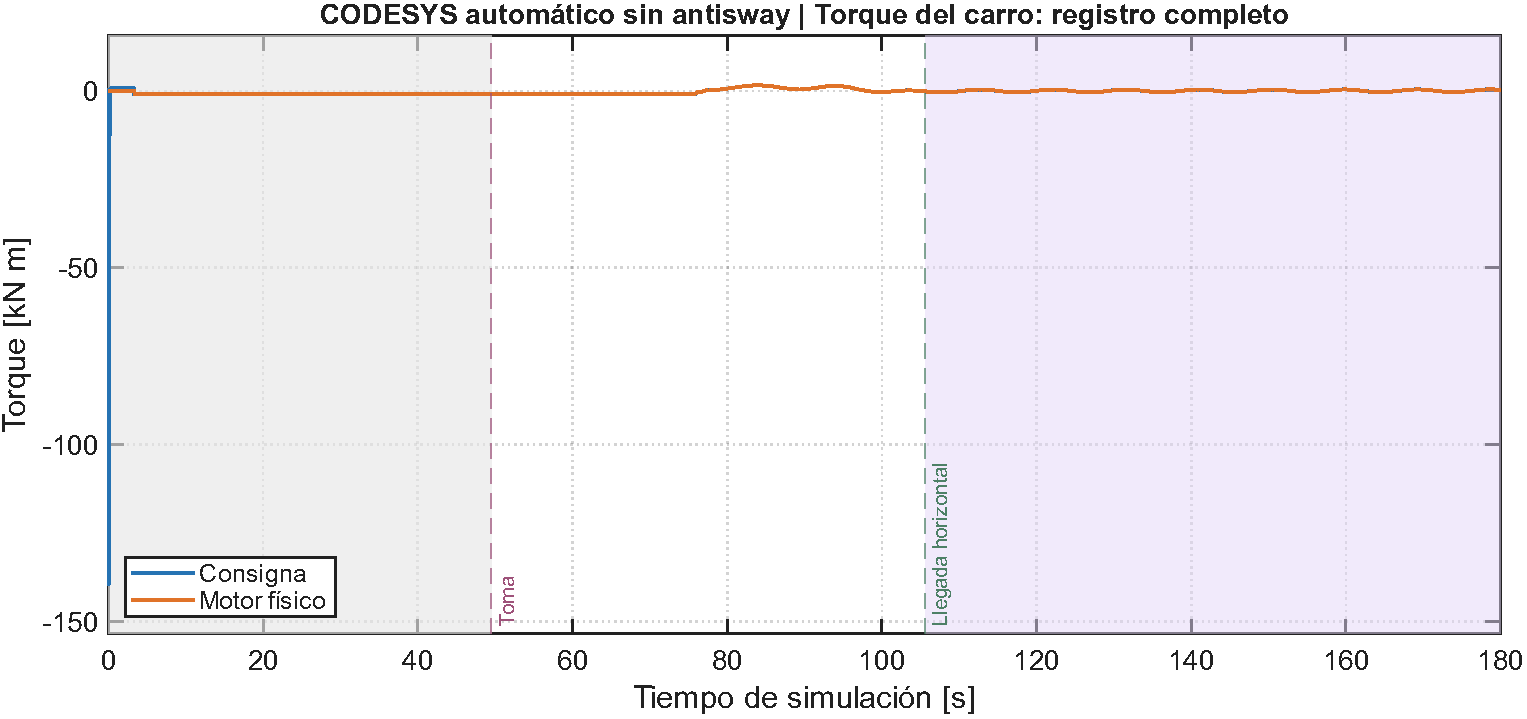
\includegraphics[width=0.98\textwidth]{graficas_individuales/automatico_sin_tx.pdf}
\caption{CODESYS automático sin antisway: Consigna y torque físico del motor del carro en el intervalo representado, incluido el arranque.}\label{fig:individual_automatico_sin_tx}
\end{figure}

\begin{figure}[!htbp]
\centering
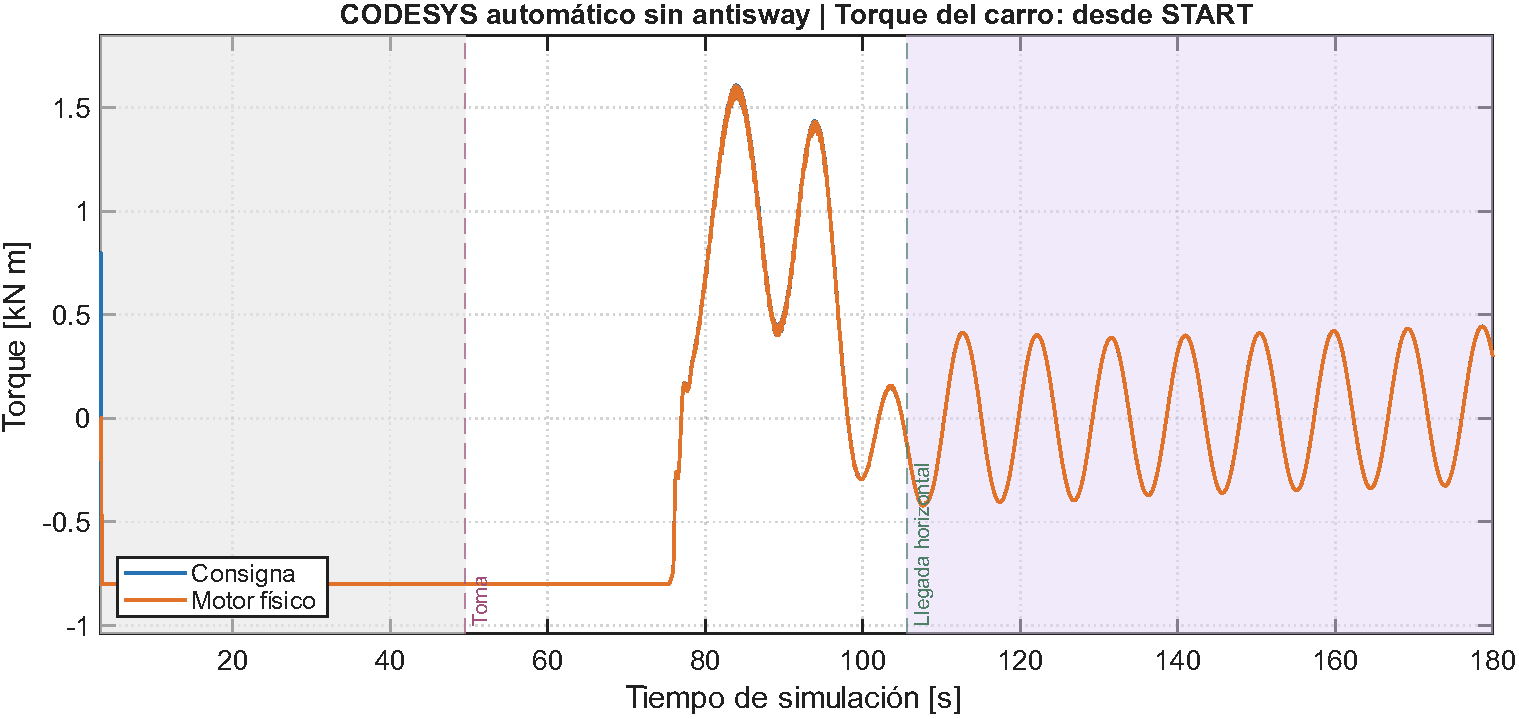
\includegraphics[width=0.98\textwidth]{graficas_individuales/automatico_sin_tx_zoom.pdf}
\caption{CODESYS automático sin antisway: Consigna y torque físico del motor del carro desde START; la escala completa del arranque se conserva en una figura independiente.}\label{fig:individual_automatico_sin_tx_zoom}
\end{figure}

\begin{figure}[!htbp]
\centering
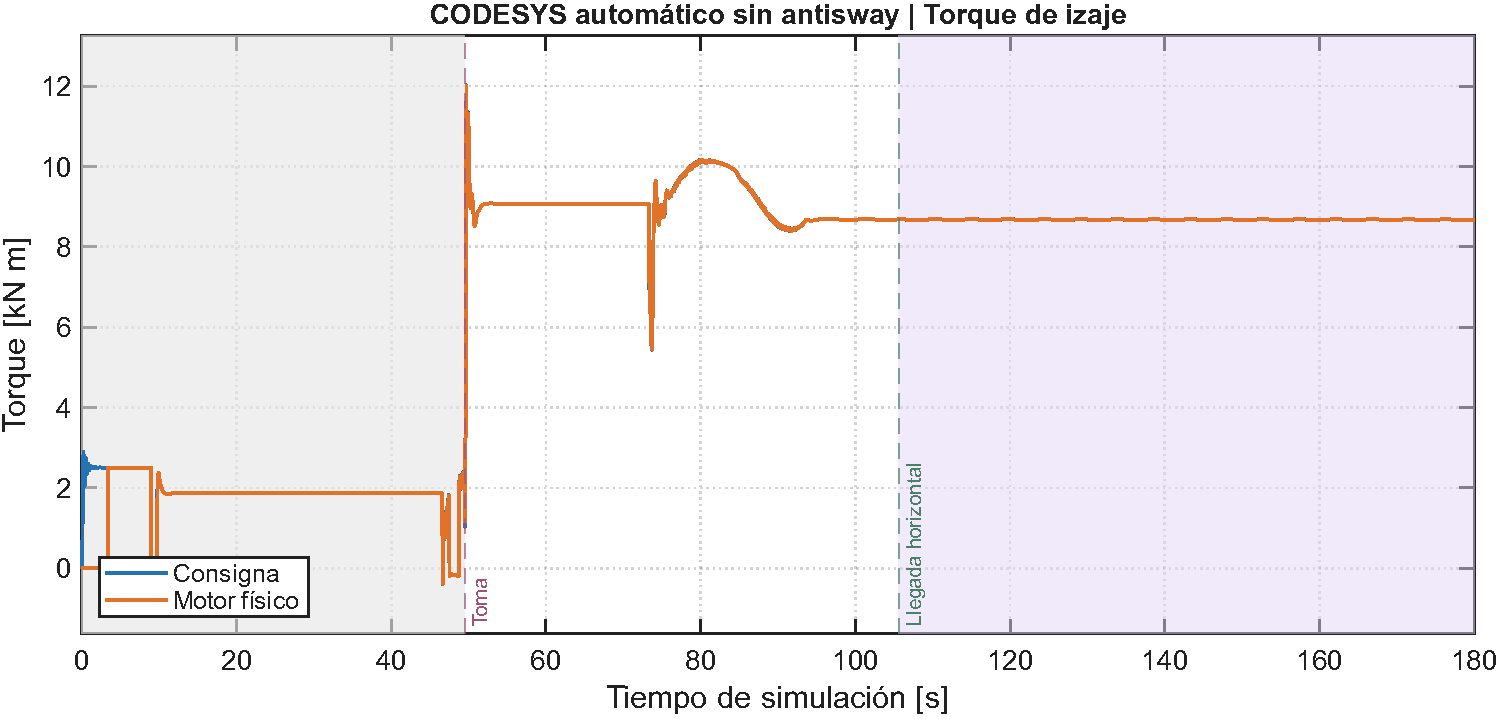
\includegraphics[width=0.98\textwidth]{graficas_individuales/automatico_sin_ty.pdf}
\caption{CODESYS automático sin antisway: Consigna del controlador y torque físico del motor de izaje.}\label{fig:individual_automatico_sin_ty}
\end{figure}

\begin{figure}[!htbp]
\centering
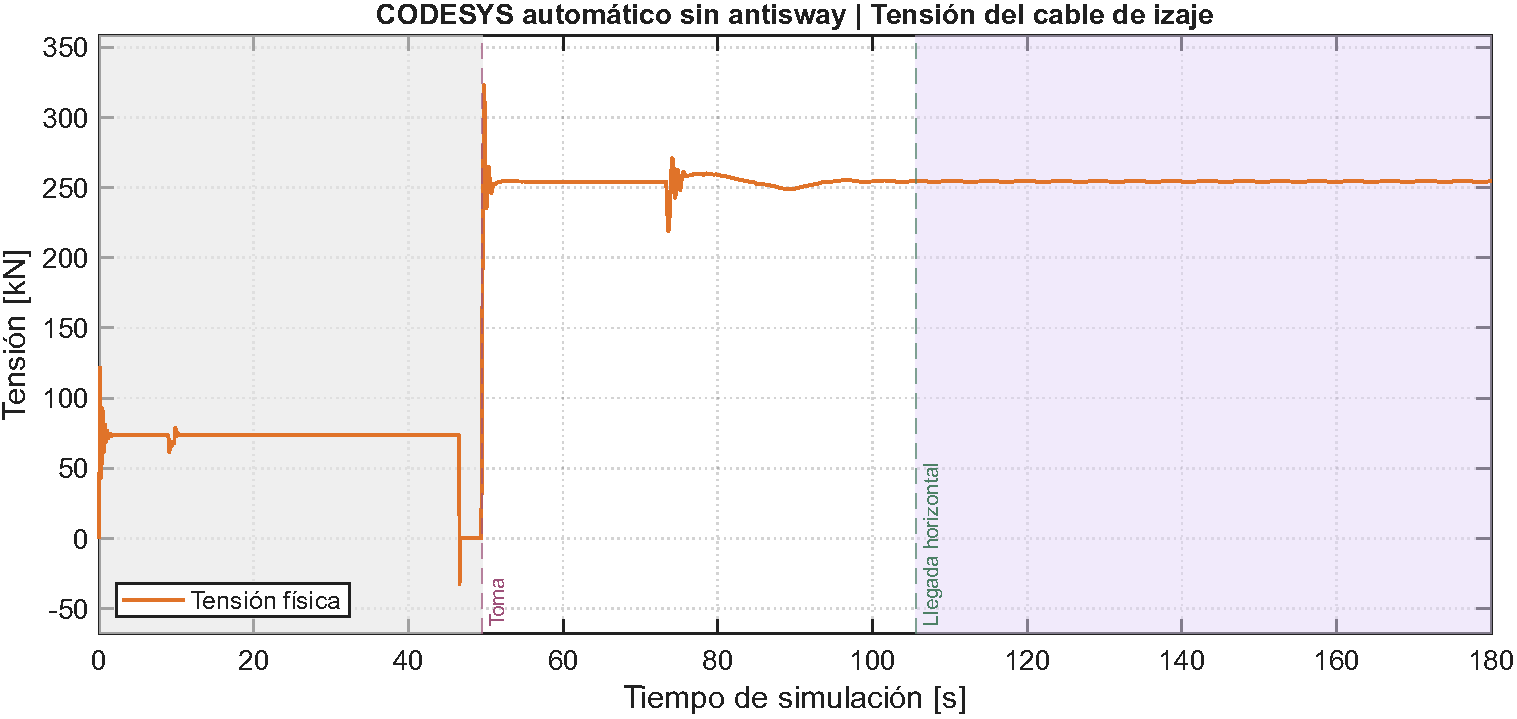
\includegraphics[width=0.98\textwidth]{graficas_individuales/automatico_sin_tension.pdf}
\caption{CODESYS automático sin antisway: Tensión física del cable de izaje.}\label{fig:individual_automatico_sin_tension}
\end{figure}

\begin{figure}[!htbp]
\centering
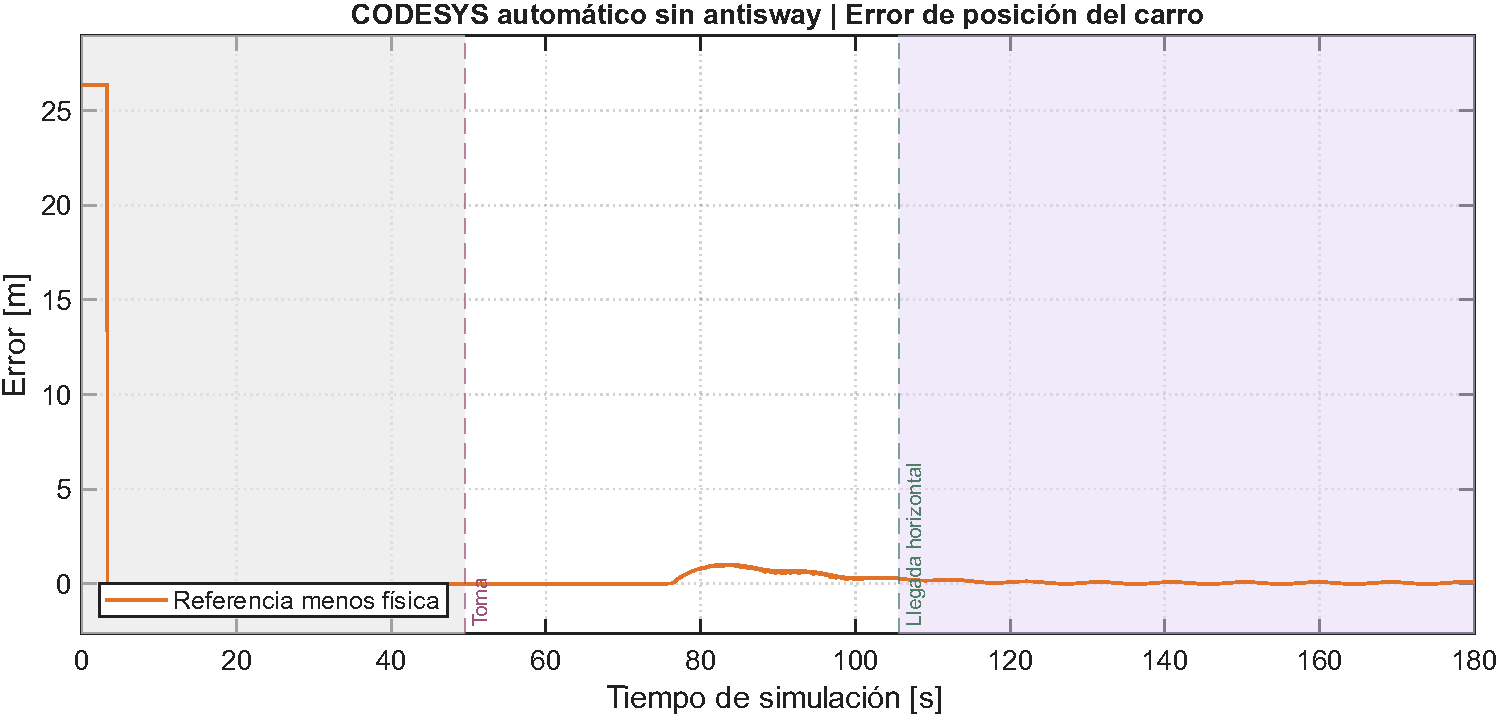
\includegraphics[width=0.98\textwidth]{graficas_individuales/automatico_sin_ex.pdf}
\caption{CODESYS automático sin antisway: Error horizontal, calculado como referencia menos posición física.}\label{fig:individual_automatico_sin_ex}
\end{figure}

\begin{figure}[!htbp]
\centering
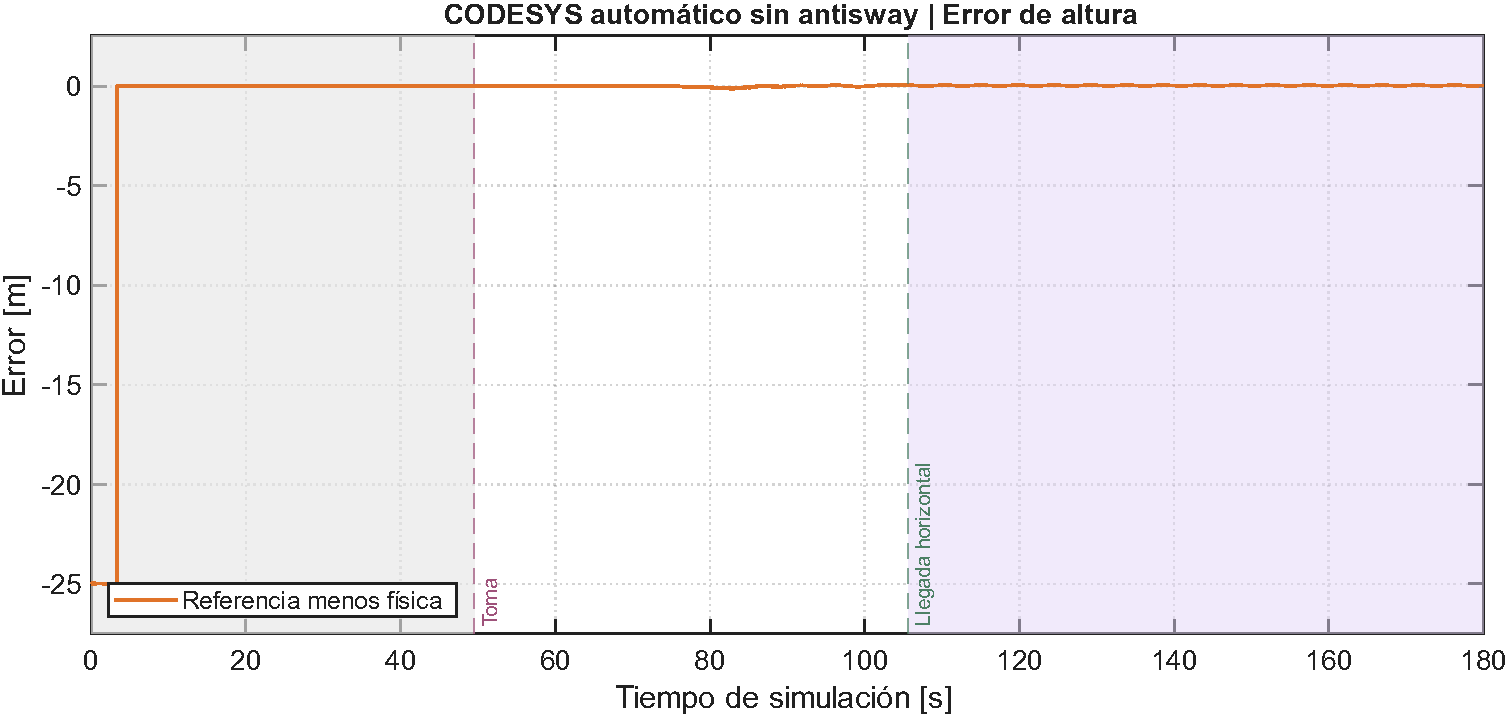
\includegraphics[width=0.98\textwidth]{graficas_individuales/automatico_sin_ey.pdf}
\caption{CODESYS automático sin antisway: Error de altura, calculado como referencia menos altura física.}\label{fig:individual_automatico_sin_ey}
\end{figure}

\begin{figure}[!htbp]
\centering
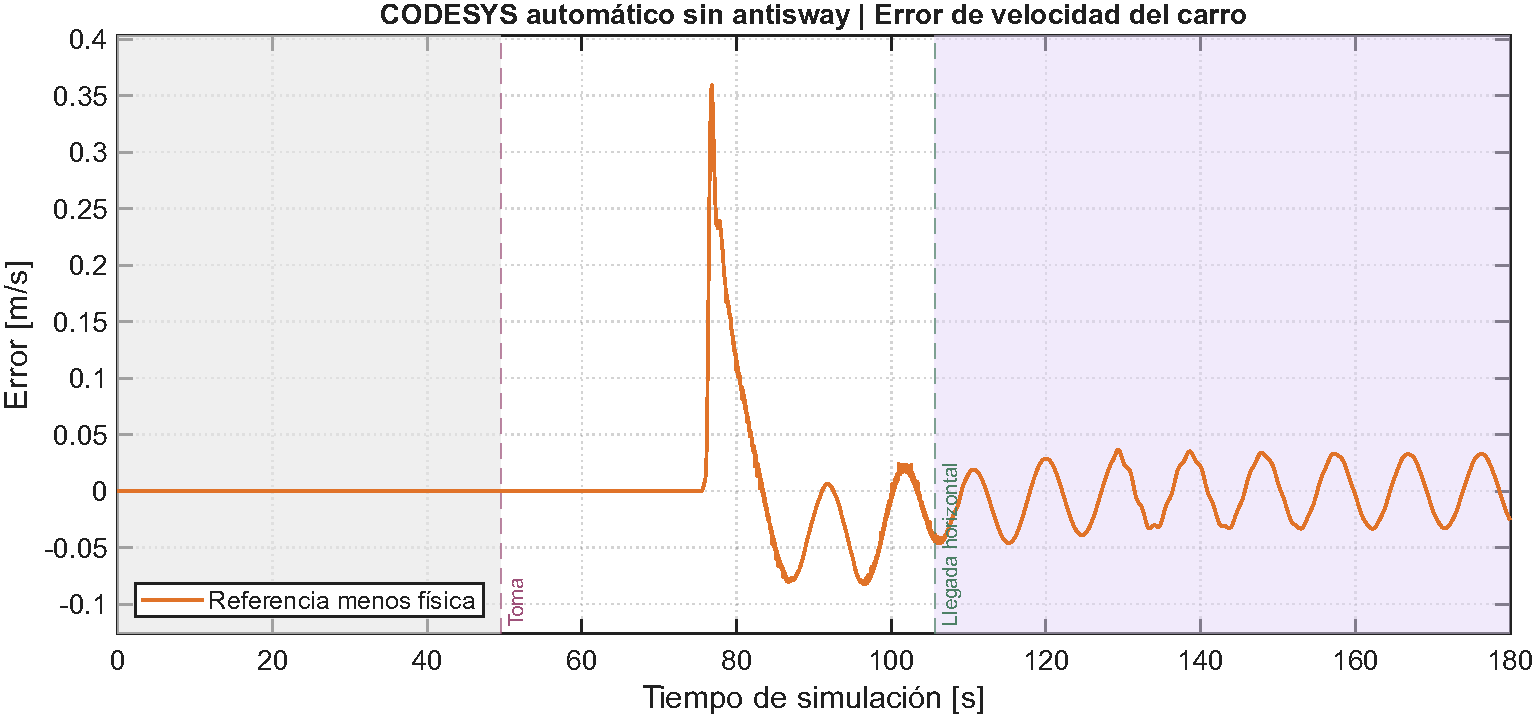
\includegraphics[width=0.98\textwidth]{graficas_individuales/automatico_sin_evx.pdf}
\caption{CODESYS automático sin antisway: Error de velocidad del carro, calculado como referencia menos velocidad física.}\label{fig:individual_automatico_sin_evx}
\end{figure}

\begin{figure}[!htbp]
\centering
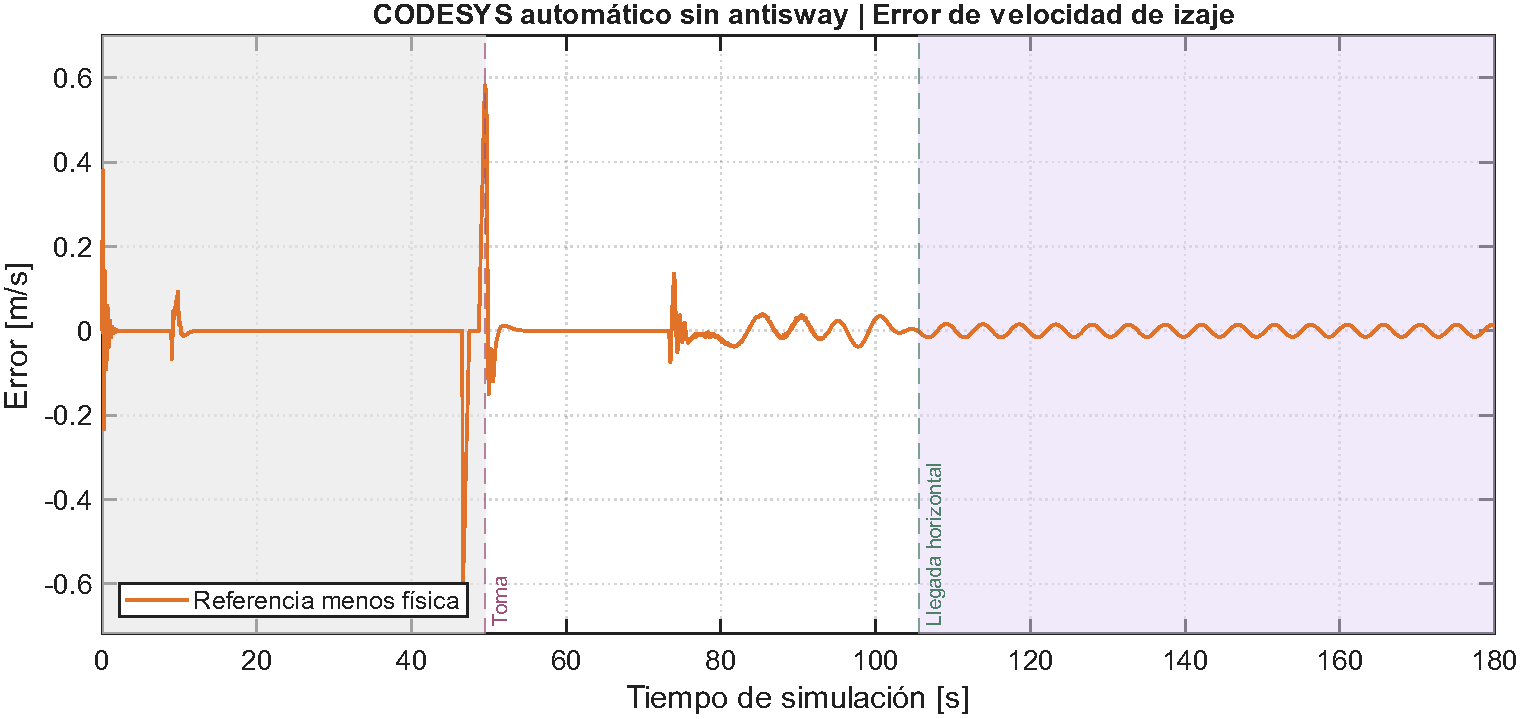
\includegraphics[width=0.98\textwidth]{graficas_individuales/automatico_sin_evy.pdf}
\caption{CODESYS automático sin antisway: Error de velocidad de izaje, calculado como referencia menos velocidad física.}\label{fig:individual_automatico_sin_evy}
\end{figure}

\begin{figure}[!htbp]
\centering
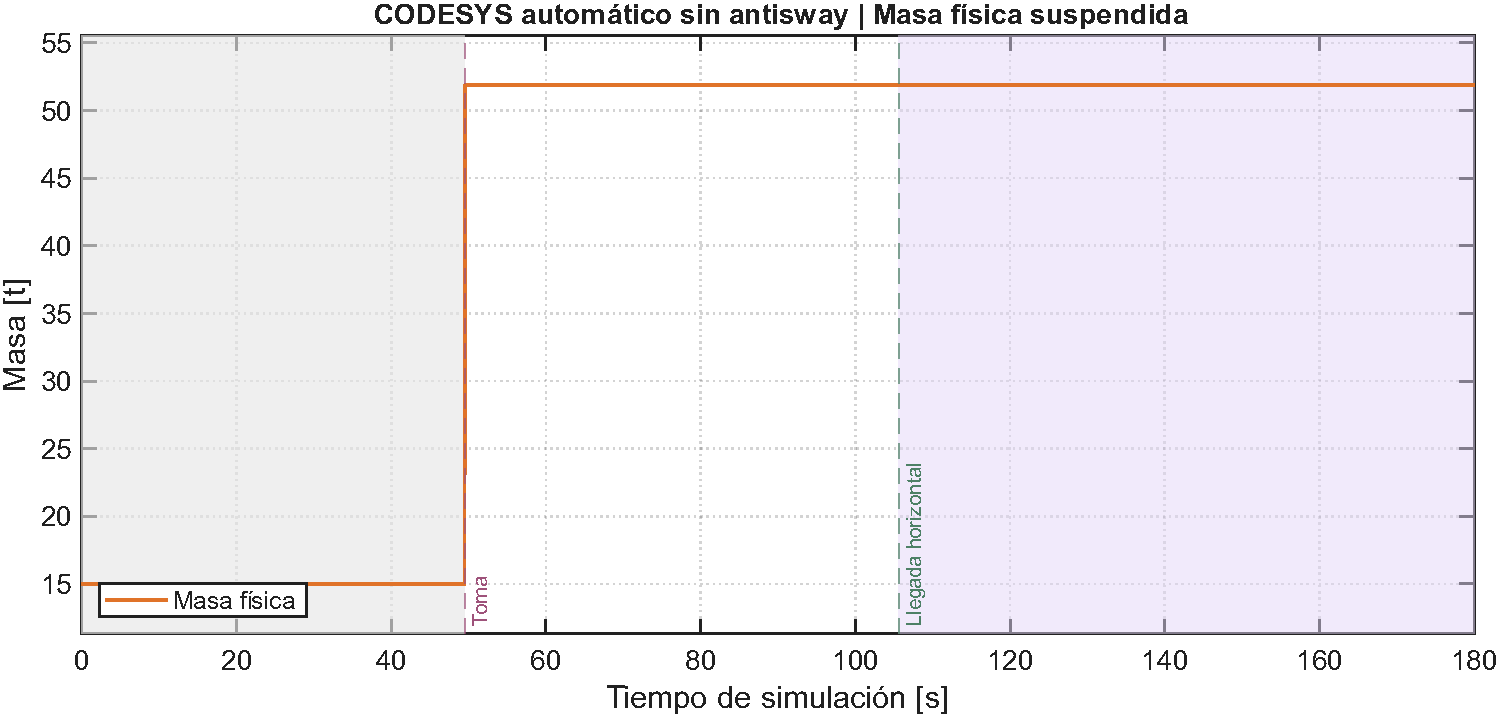
\includegraphics[width=0.98\textwidth]{graficas_individuales/automatico_sin_masa.pdf}
\caption{CODESYS automático sin antisway: Masa física suspendida: 51,863 t representa conjunto cargado y 15 t corresponde al spreader vacío.}\label{fig:individual_automatico_sin_masa}
\end{figure}

\begin{figure}[!htbp]
\centering
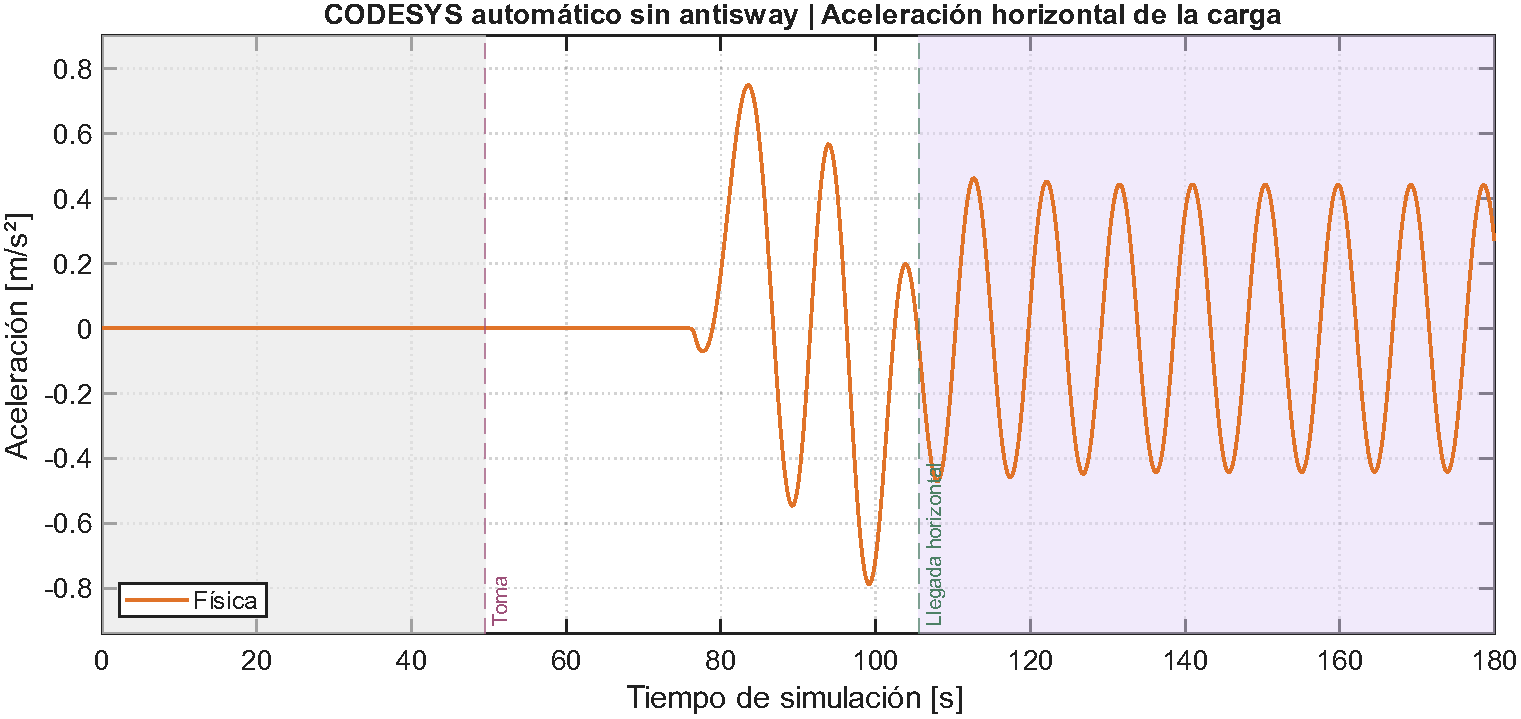
\includegraphics[width=0.98\textwidth]{graficas_individuales/automatico_sin_ax_carga.pdf}
\caption{CODESYS automático sin antisway: Aceleración horizontal física de la carga; se conservan las oscilaciones registradas.}\label{fig:individual_automatico_sin_ax_carga}
\end{figure}

\clearpage
\subsection{CODESYS automático con antisway: apoyo con descarga física bloqueada}
START ocurrió a $3.24~\mathrm{s}$, manual a $3.76~\mathrm{s}$ y cierre solicitado a $46.64~\mathrm{s}$. La masa cargada se confirmó a $49.52~\mathrm{s}$ y el despegue a $50.00~\mathrm{s}$. Automático se solicitó a $75.32~\mathrm{s}$ y fue observado por el operador a $75.40~\mathrm{s}$; el monitor de modo registra automático a $75.44~\mathrm{s}$. La llegada horizontal ocurrió a $105.76~\mathrm{s}$. Manual se solicitó a $133.20~\mathrm{s}$; el monitor registra el cambio a $133.24~\mathrm{s}$ y el operador lo confirmó a $133.56~\mathrm{s}$. Se distinguen estos tiempos porque la lectura y confirmación del operador añaden retardo respecto del monitor.

Con antisway se habilitó el avance del descenso y se alcanzó apoyo con solicitud de apertura a $169.24~\mathrm{s}$. Se permitió continuar más allá de tres minutos. Sin embargo, la planta mantuvo la carga: el diagnóstico a $272.52~\mathrm{s}$ mostró twistlocks abiertos y estado de carga vacío en el PLC, con contacto confirmado, mientras la masa física seguía siendo $51\,863~\mathrm{kg}$. Después de más de 100 s sin transferencia física en apoyo, se efectuó parada controlada de diagnóstico a $279.52~\mathrm{s}$.

\begin{figure}[!htbp]
\centering
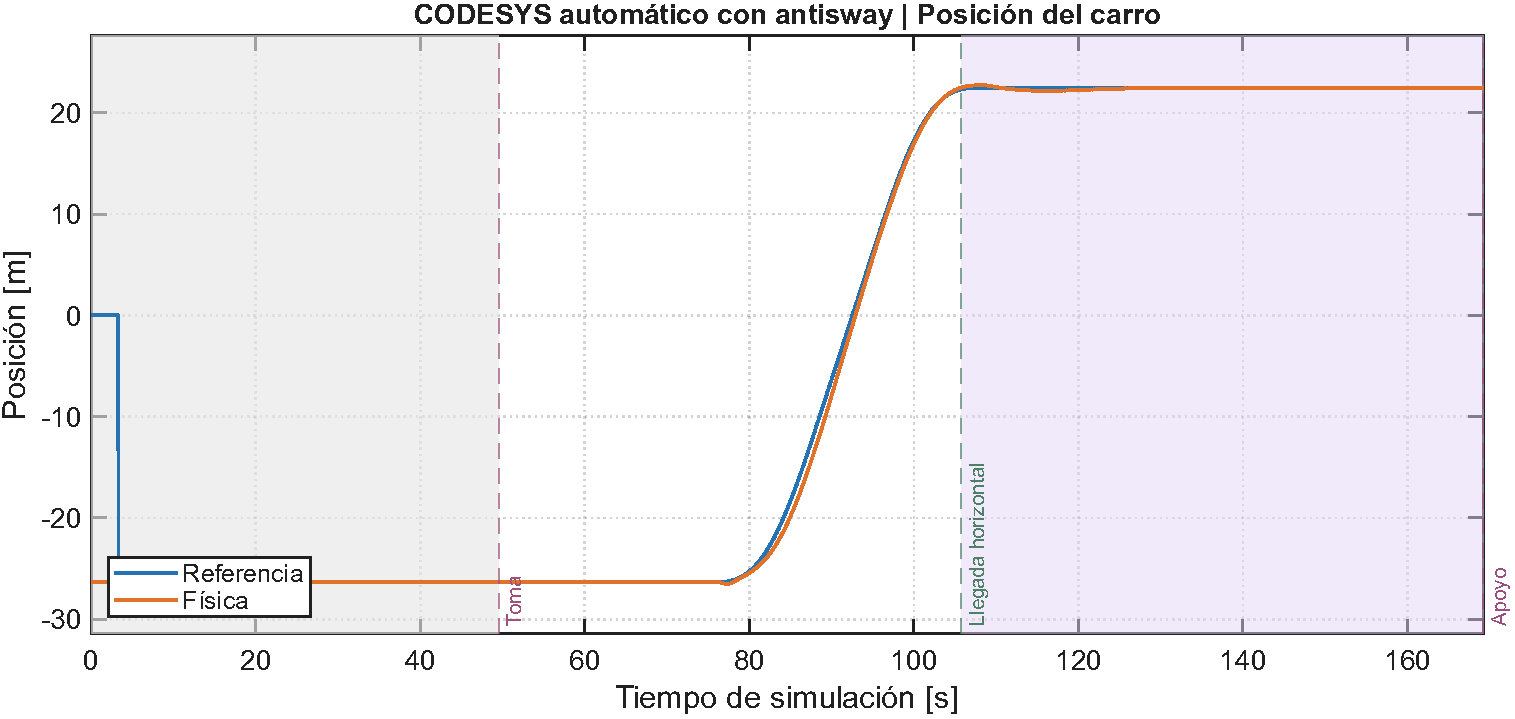
\includegraphics[width=0.98\textwidth]{graficas_individuales/automatico_con_x.pdf}
\caption{CODESYS automático con antisway: Posición del carro: referencia y evolución física.}\label{fig:individual_automatico_con_x}
\end{figure}

\begin{figure}[!htbp]
\centering
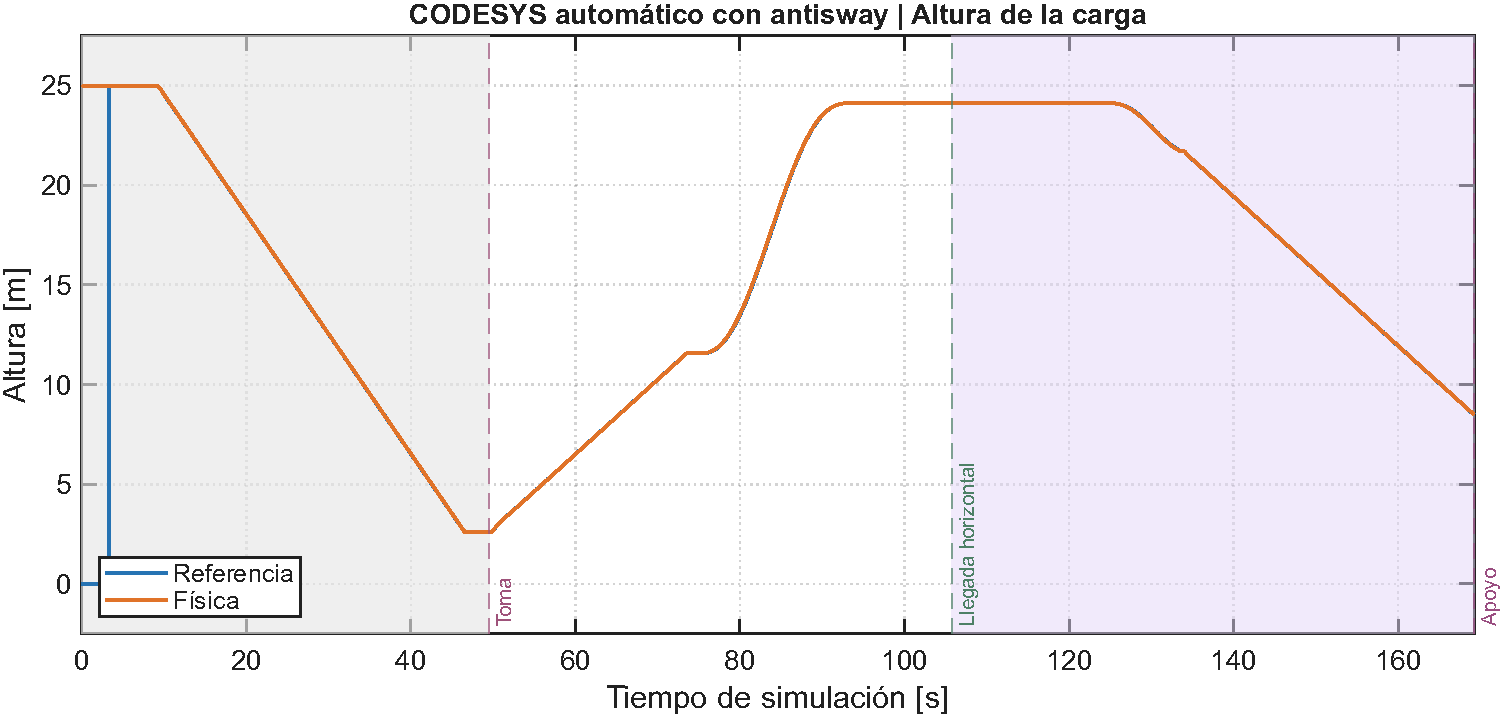
\includegraphics[width=0.98\textwidth]{graficas_individuales/automatico_con_y.pdf}
\caption{CODESYS automático con antisway: Altura de la carga: referencia y evolución física.}\label{fig:individual_automatico_con_y}
\end{figure}

\begin{figure}[!htbp]
\centering
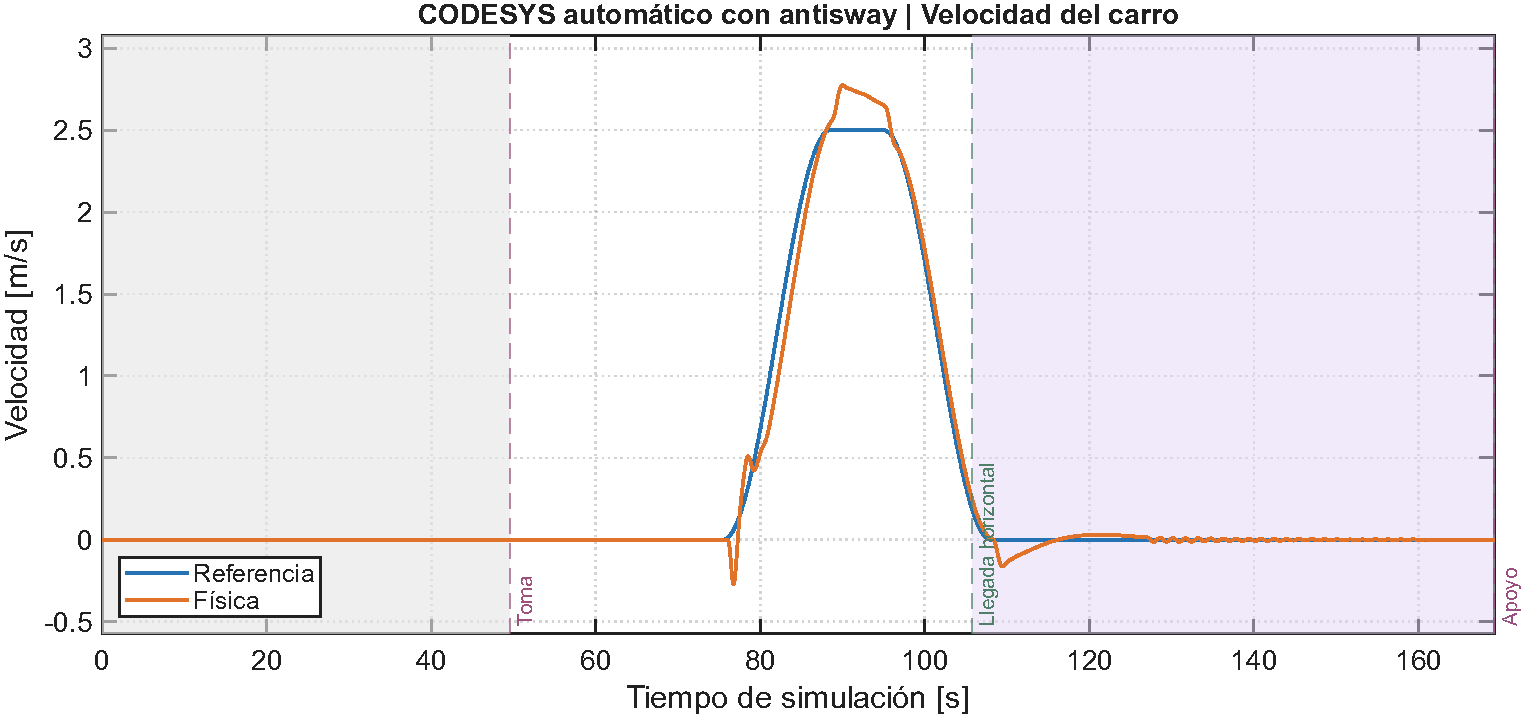
\includegraphics[width=0.98\textwidth]{graficas_individuales/automatico_con_vx.pdf}
\caption{CODESYS automático con antisway: Velocidad del carro: referencia y señal física.}\label{fig:individual_automatico_con_vx}
\end{figure}

\begin{figure}[!htbp]
\centering
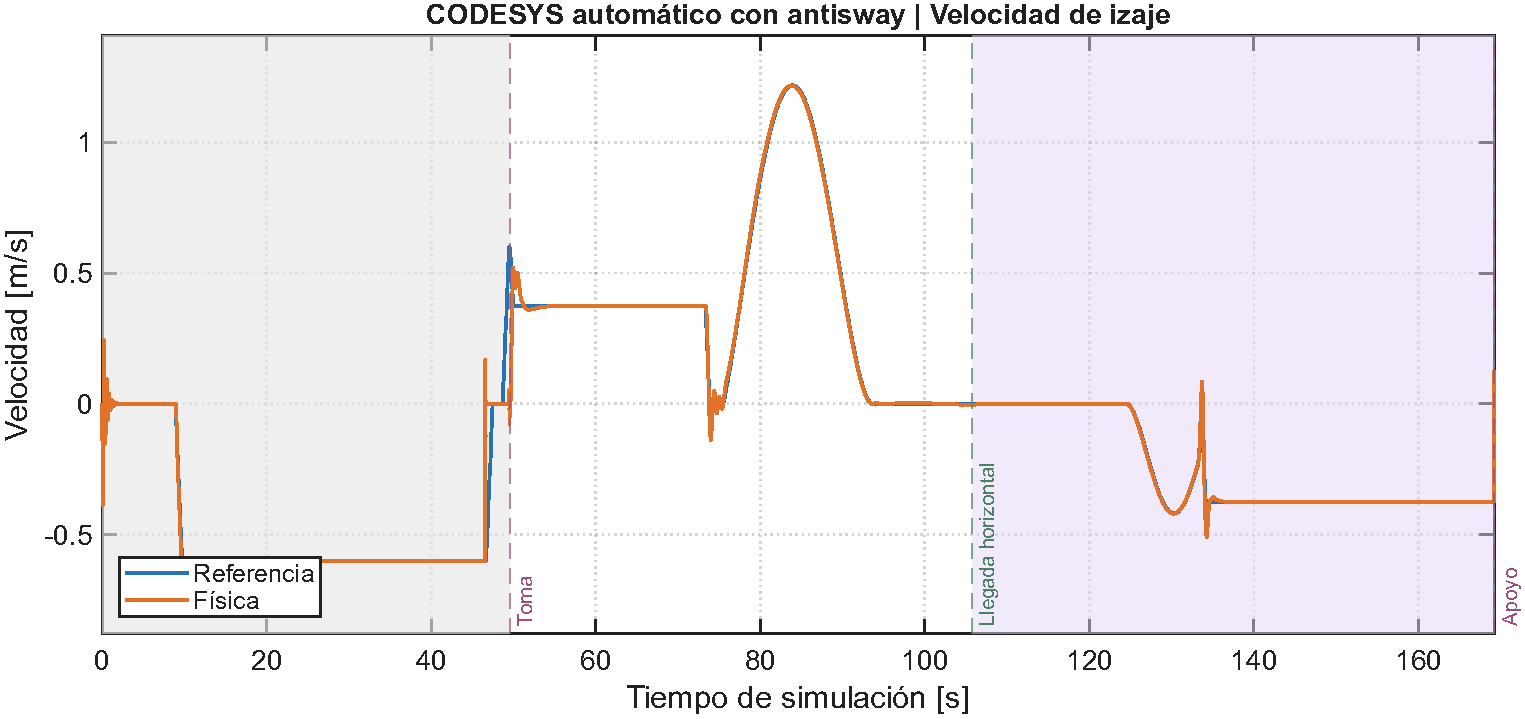
\includegraphics[width=0.98\textwidth]{graficas_individuales/automatico_con_vy.pdf}
\caption{CODESYS automático con antisway: Velocidad de izaje: referencia y señal física.}\label{fig:individual_automatico_con_vy}
\end{figure}

\begin{figure}[!htbp]
\centering
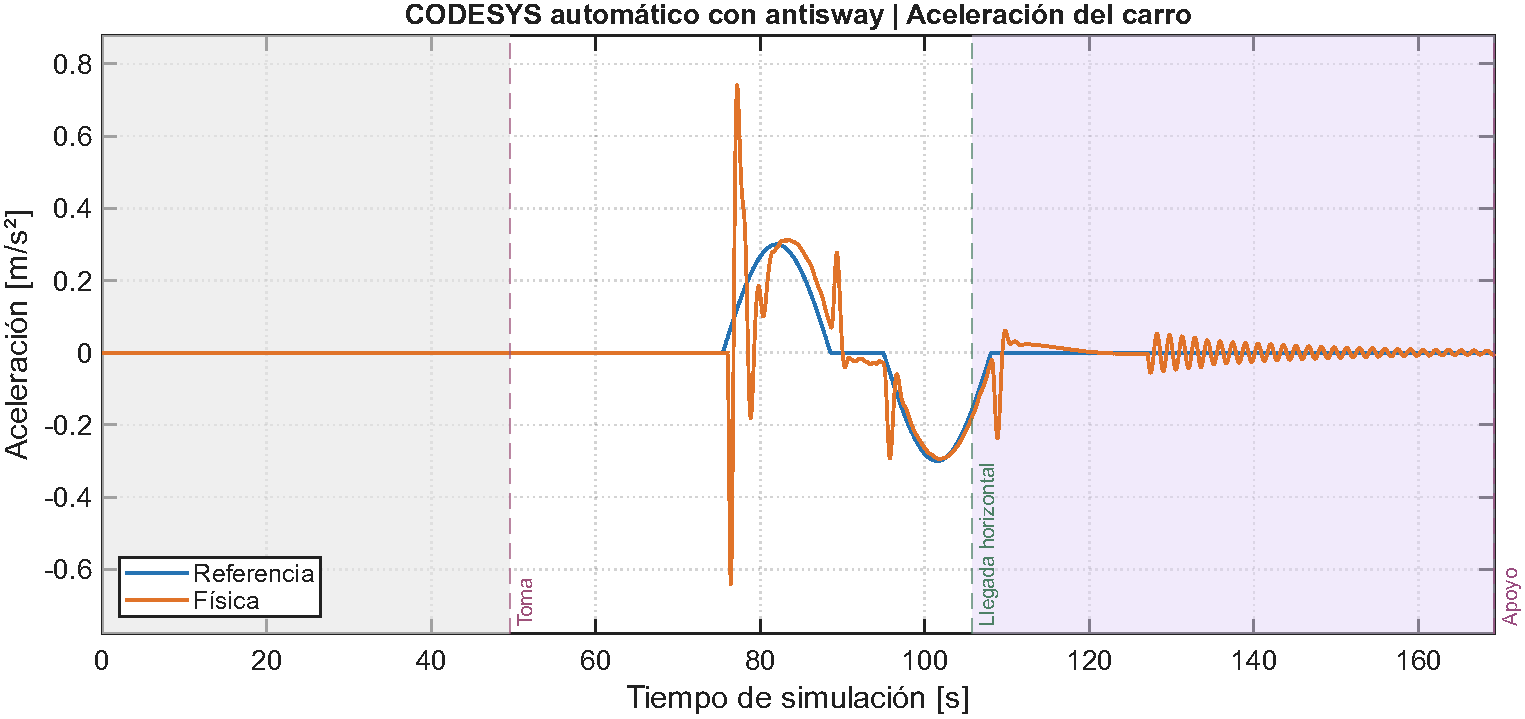
\includegraphics[width=0.98\textwidth]{graficas_individuales/automatico_con_ax.pdf}
\caption{CODESYS automático con antisway: Aceleración del carro: referencia y señal física.}\label{fig:individual_automatico_con_ax}
\end{figure}

\begin{figure}[!htbp]
\centering
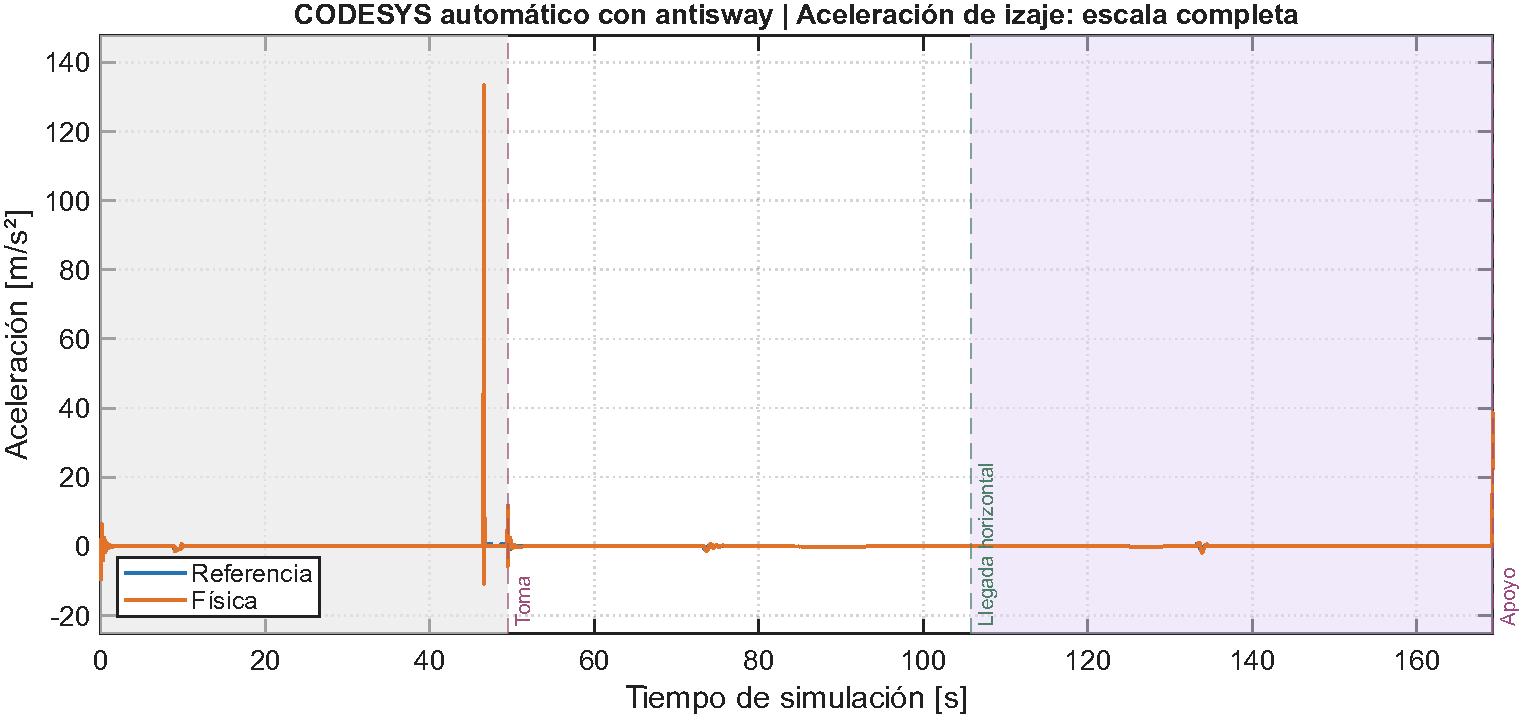
\includegraphics[width=0.98\textwidth]{graficas_individuales/automatico_con_ay.pdf}
\caption{CODESYS automático con antisway: Aceleración de izaje en escala completa; se conservan los picos de contacto y arranque.}\label{fig:individual_automatico_con_ay}
\end{figure}

\begin{figure}[!htbp]
\centering
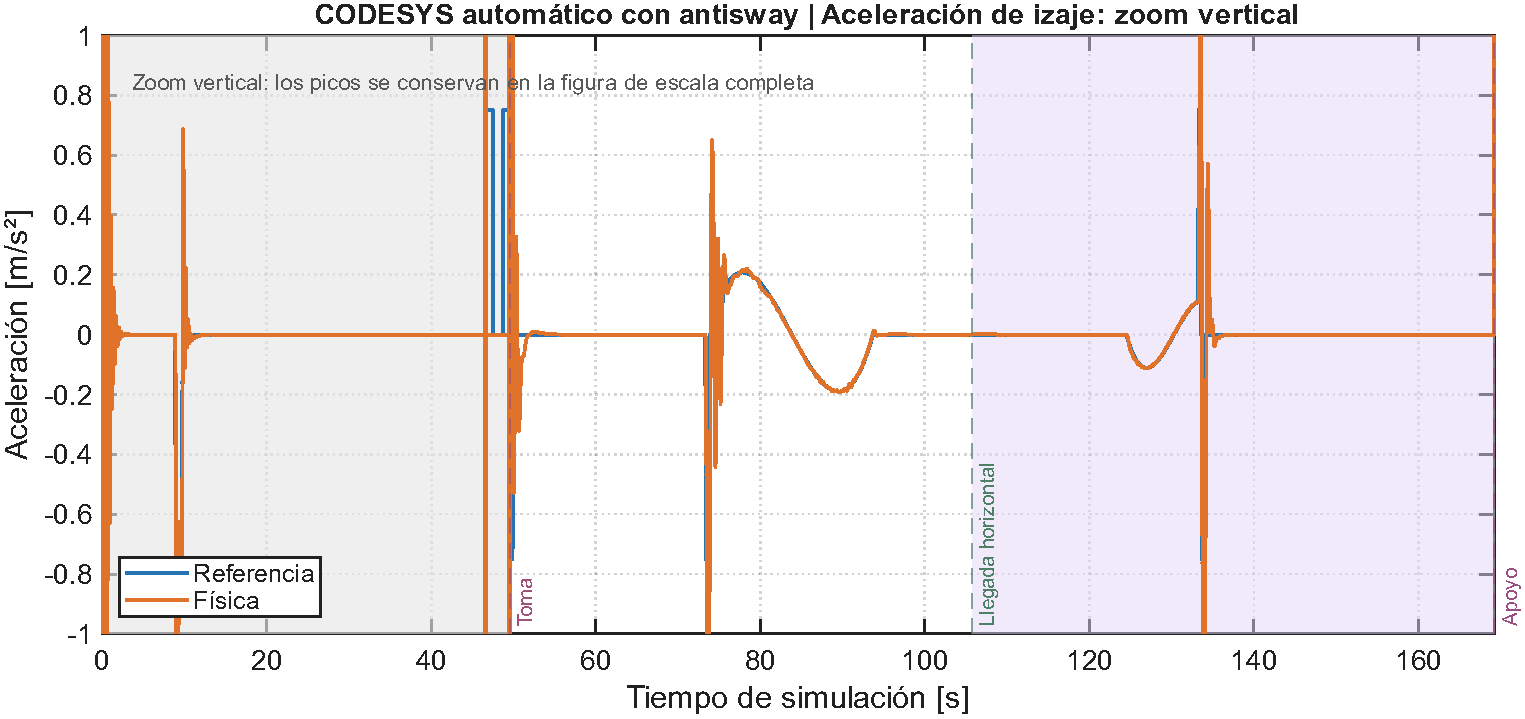
\includegraphics[width=0.98\textwidth]{graficas_individuales/automatico_con_ay_zoom.pdf}
\caption{CODESYS automático con antisway: Aceleración de izaje con zoom vertical entre $-1$ y $+1~\mathrm{m/s^2}$ para observar su evolución temporal. Los picos que exceden este intervalo permanecen visibles en la figura de escala completa; no se filtraron las señales.}\label{fig:individual_automatico_con_ay_zoom}
\end{figure}

\begin{figure}[!htbp]
\centering
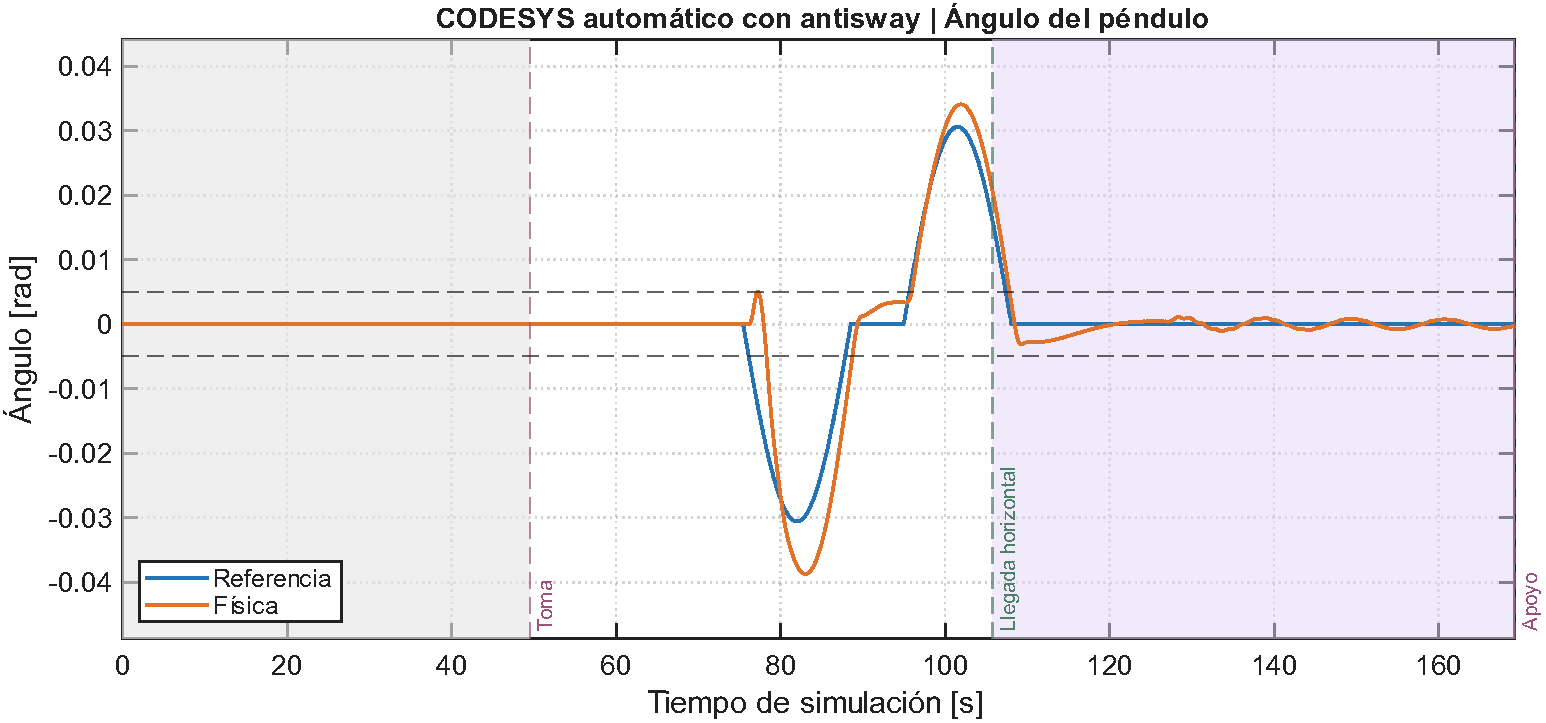
\includegraphics[width=0.98\textwidth]{graficas_individuales/automatico_con_theta.pdf}
\caption{CODESYS automático con antisway: Ángulo físico y de referencia del péndulo. Las líneas horizontales señalan los umbrales angulares del descenso.}\label{fig:individual_automatico_con_theta}
\end{figure}

\begin{figure}[!htbp]
\centering
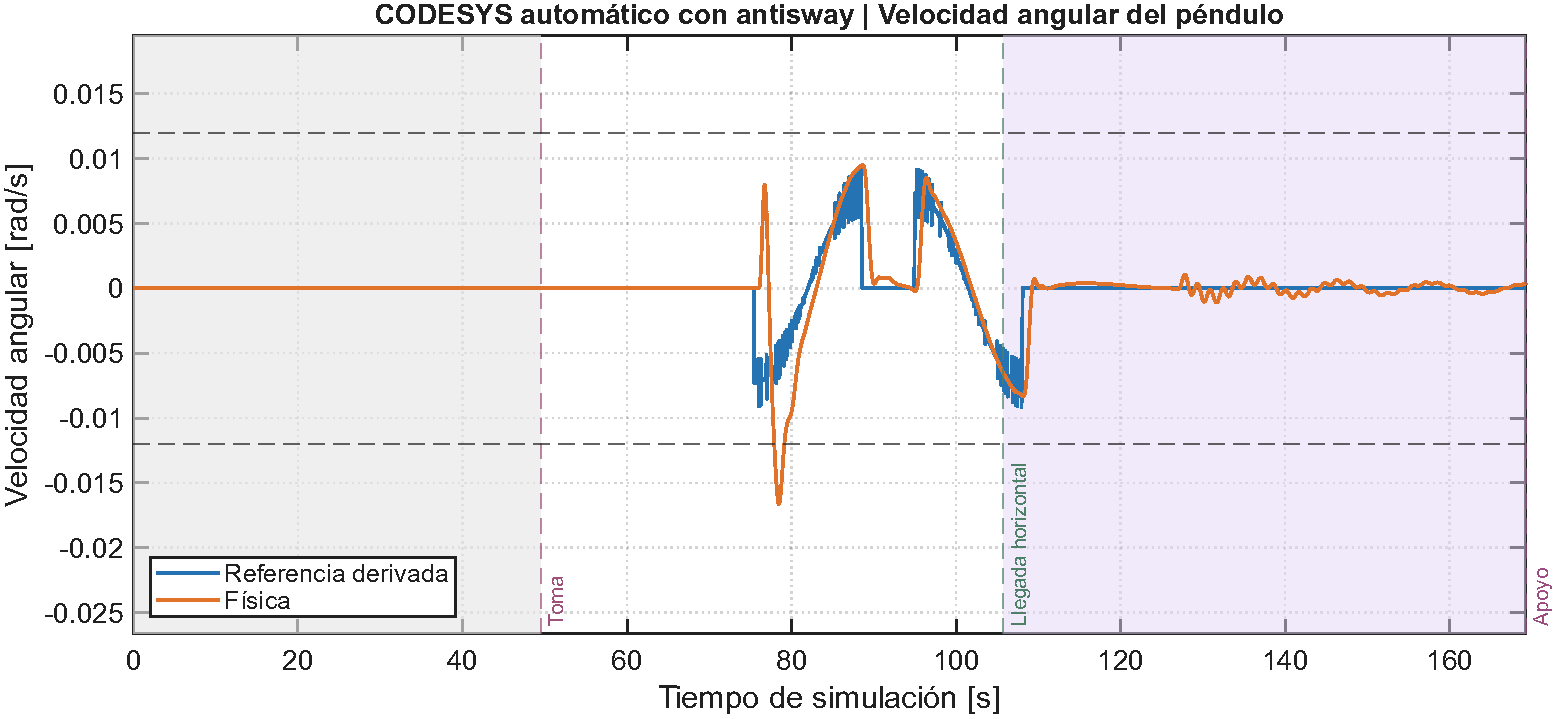
\includegraphics[width=0.98\textwidth]{graficas_individuales/automatico_con_omega.pdf}
\caption{CODESYS automático con antisway: Velocidad angular física y referencia derivada numéricamente; se distinguen ambas fuentes. Las líneas horizontales indican los umbrales del descenso.}\label{fig:individual_automatico_con_omega}
\end{figure}

\begin{figure}[!htbp]
\centering
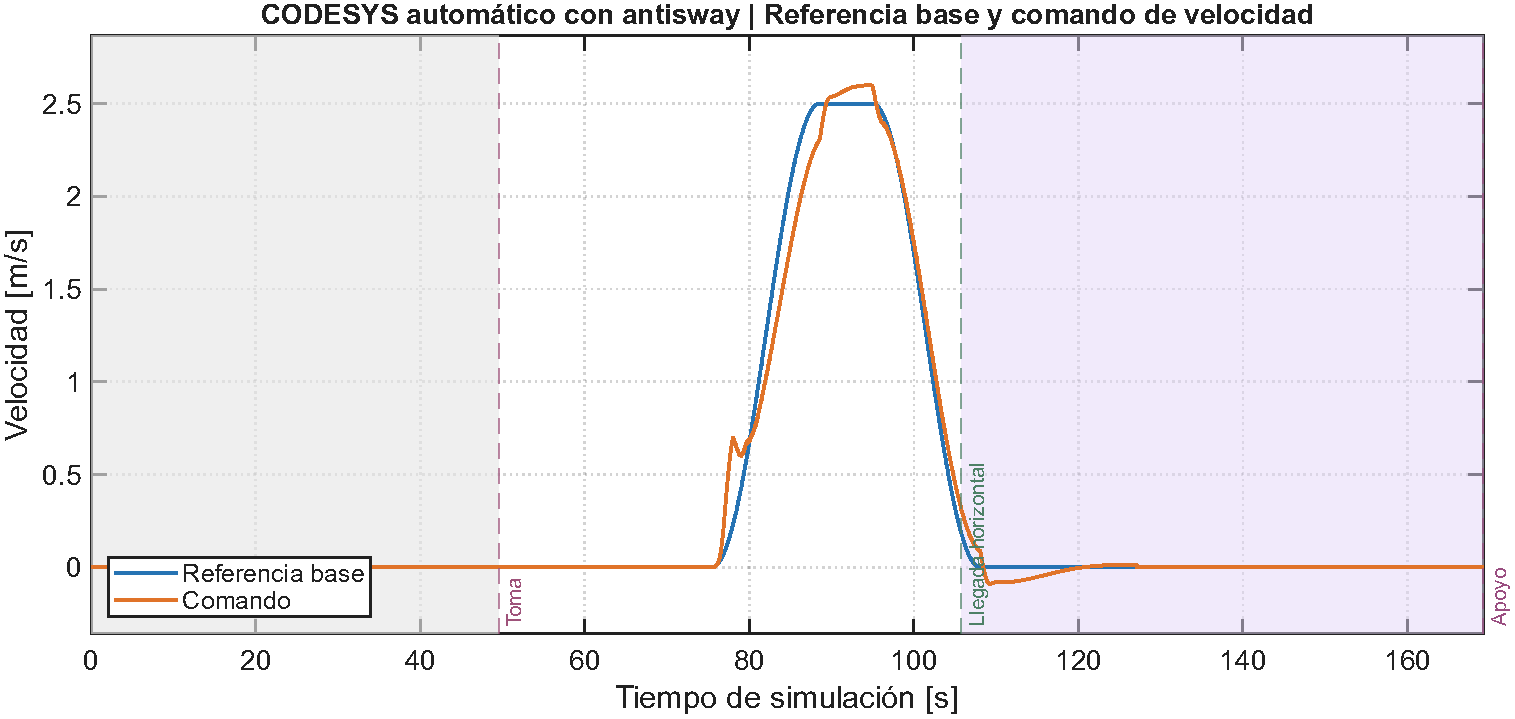
\includegraphics[width=0.98\textwidth]{graficas_individuales/automatico_con_vcmd.pdf}
\caption{CODESYS automático con antisway: Referencia base y comando de velocidad; su diferencia corresponde a la contribución antisway efectiva en el sumador.}\label{fig:individual_automatico_con_vcmd}
\end{figure}

\begin{figure}[!htbp]
\centering
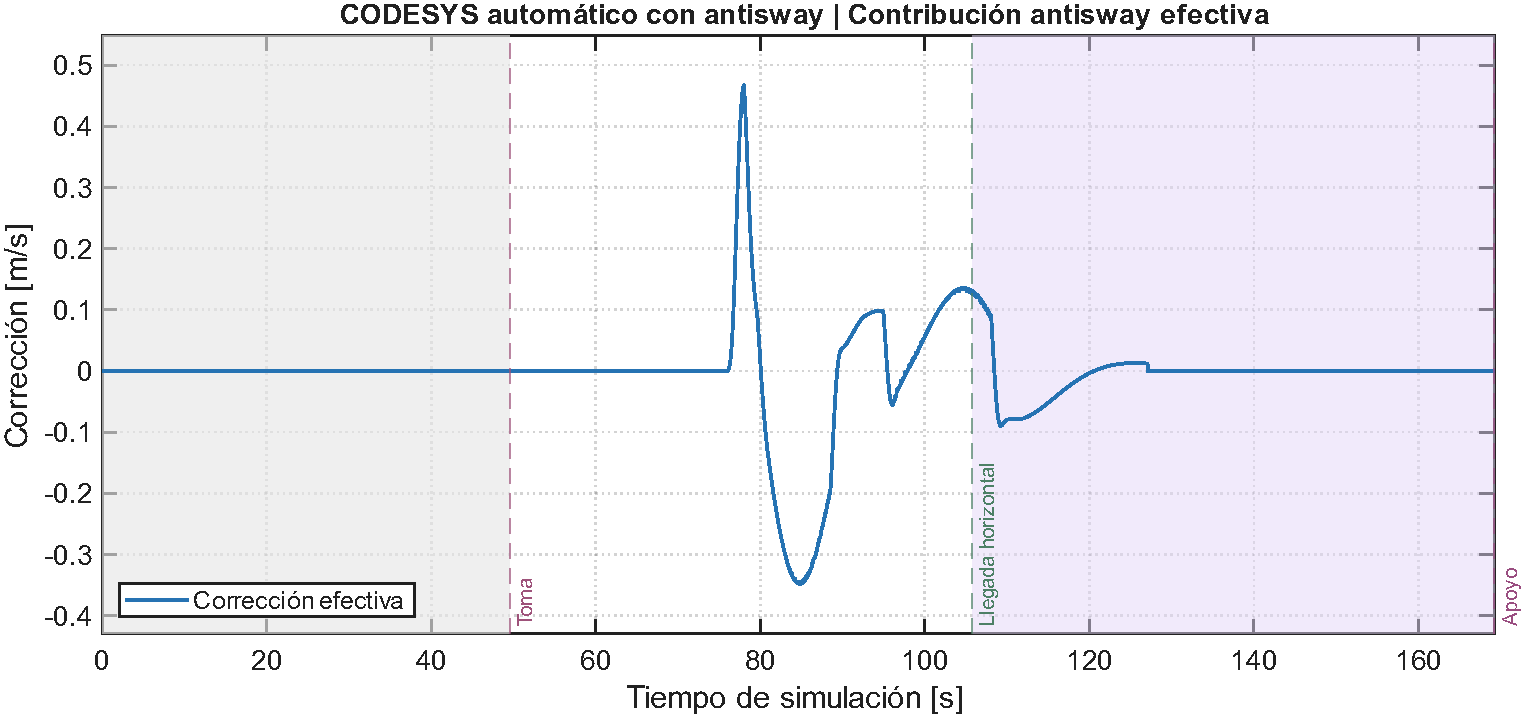
\includegraphics[width=0.98\textwidth]{graficas_individuales/automatico_con_sw.pdf}
\caption{CODESYS automático con antisway: Contribución antisway efectivamente sumada al comando de velocidad.}\label{fig:individual_automatico_con_sw}
\end{figure}

La contribución antisway máxima nativa fue $0.46702~\mathrm{m/s}$, verificada sobre $279\,521$ muestras. El carro terminó en $22.43043~\mathrm{m}$ y la carga en $8.48983~\mathrm{m}$; el error horizontal fue $0.02957~\mathrm{m}$. El origen disminuyó $2.59~\mathrm{m}$, pero el destino no aumentó. La proximidad al destino y el estado vacío del PLC no reemplazan esas comprobaciones físicas.

La lógica física de descarga exige simultáneamente apertura, contacto, velocidad vertical pequeña y desactivación de la histéresis de tensión. En el diagnóstico, la tensión fue aproximadamente $99.54~\mathrm{kN}$, superior al umbral de desactivación de $15.009~\mathrm{kN}$. La histéresis permaneció activa y bloqueó la transferencia del contenedor. En la espera final, la consigna de torque de izaje continúa descendiendo mientras el torque de motor alcanza una meseta próxima a -20 kN m; la diferencia entre consigna y actuación muestra que la orden adicional no se traduce en el mismo incremento de torque físico. Los errores de seguimiento crecen durante la espera final porque la referencia del PLC deja de corresponder al estado cargado que persiste en la planta; no representan una nueva maniobra de entrega completada. Esta observación complementa el diagnóstico de tensión y no constituye por sí sola identificación de la causa raíz. Ésta es la condición inmediata observada; los datos no prueban que la causa raíz pertenezca al generador de código. Debe revisarse la coordinación de apoyo, referencia de izaje y confirmación de descarga antes de atribuir el resultado a PLC Coder. No se forzaron masa, estado de carga ni umbrales para declarar entrega.

\begin{figure}[!htbp]
\centering
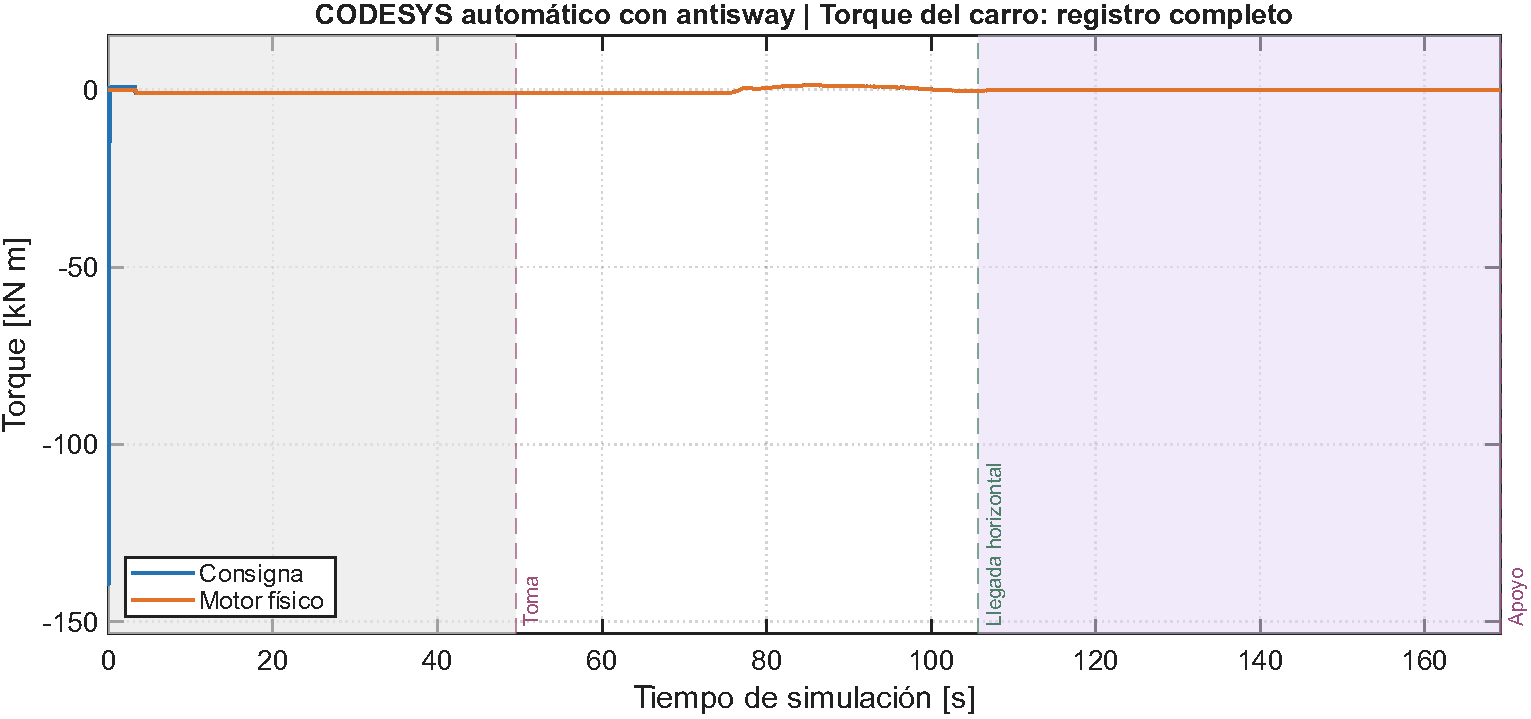
\includegraphics[width=0.98\textwidth]{graficas_individuales/automatico_con_tx.pdf}
\caption{CODESYS automático con antisway: Consigna y torque físico del motor del carro en el intervalo representado, incluido el arranque.}\label{fig:individual_automatico_con_tx}
\end{figure}

\begin{figure}[!htbp]
\centering
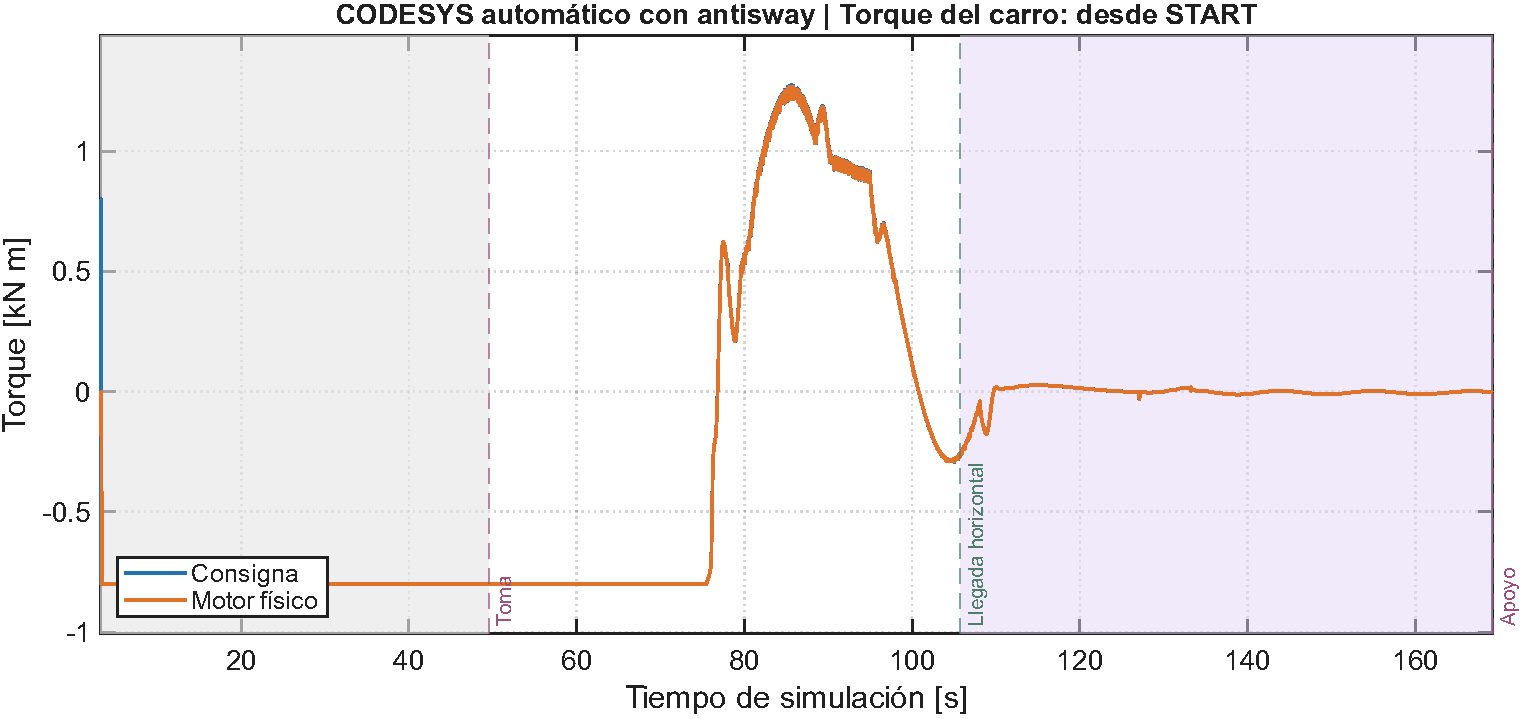
\includegraphics[width=0.98\textwidth]{graficas_individuales/automatico_con_tx_zoom.pdf}
\caption{CODESYS automático con antisway: Consigna y torque físico del motor del carro desde START; la escala completa del arranque se conserva en una figura independiente.}\label{fig:individual_automatico_con_tx_zoom}
\end{figure}

\begin{figure}[!htbp]
\centering
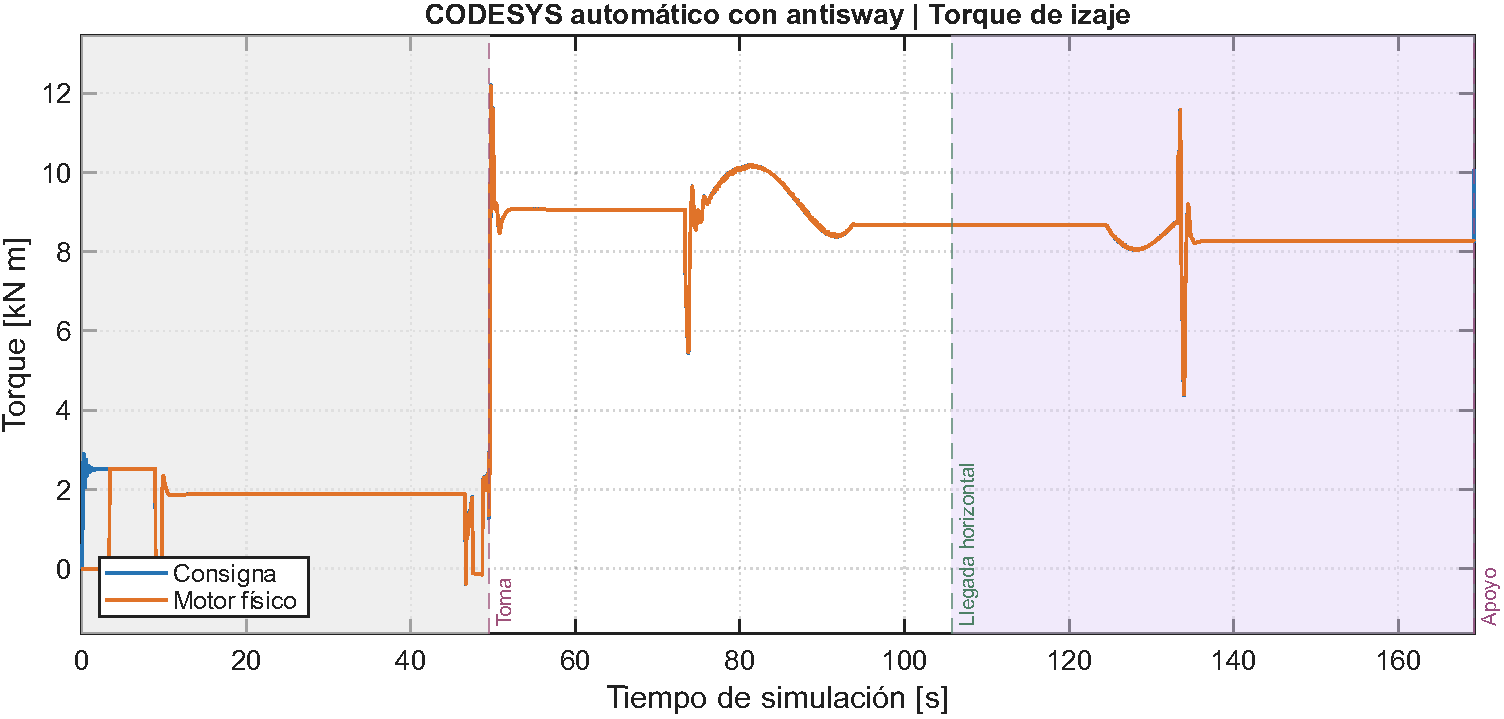
\includegraphics[width=0.98\textwidth]{graficas_individuales/automatico_con_ty.pdf}
\caption{CODESYS automático con antisway: Consigna del controlador y torque físico del motor de izaje.}\label{fig:individual_automatico_con_ty}
\end{figure}

\begin{figure}[!htbp]
\centering
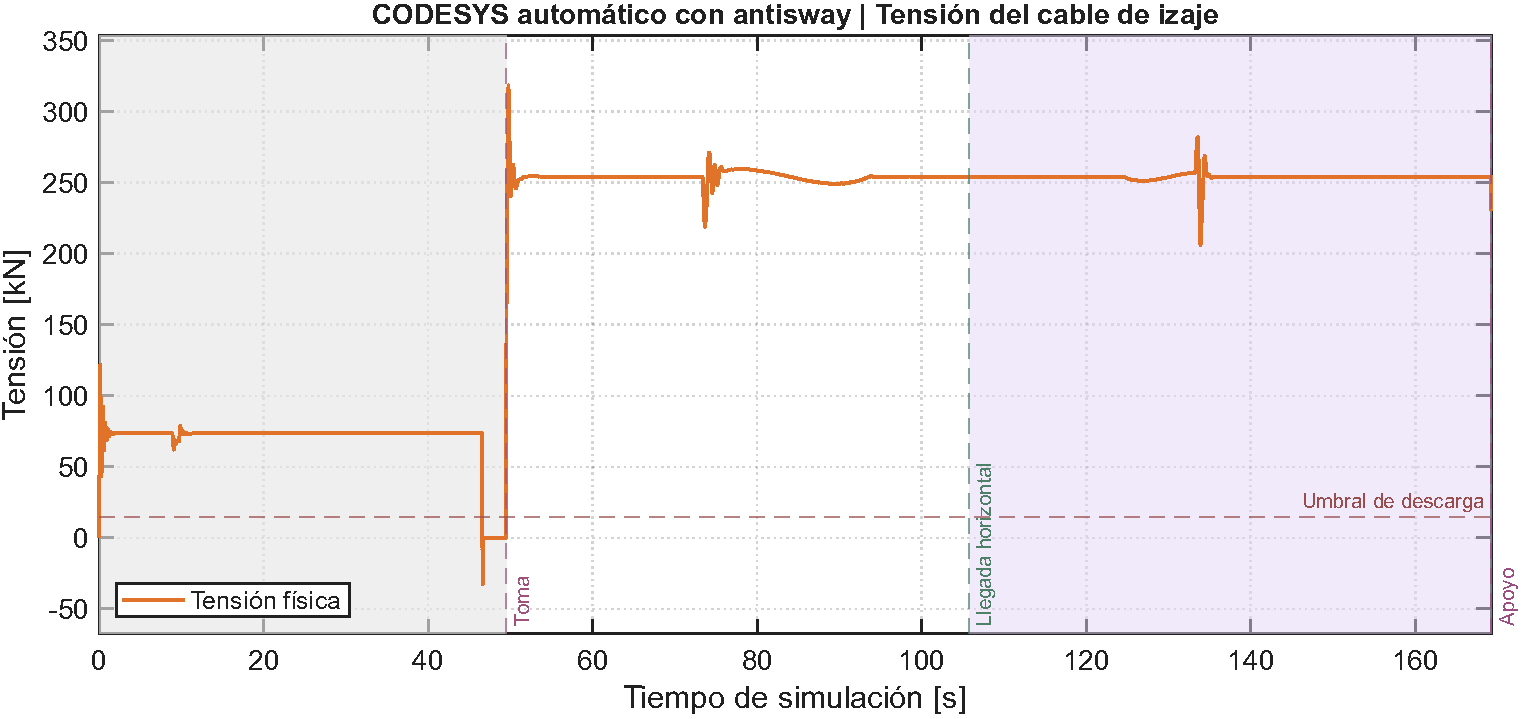
\includegraphics[width=0.98\textwidth]{graficas_individuales/automatico_con_tension.pdf}
\caption{CODESYS automático con antisway: Tensión física del cable de izaje. Se conserva el umbral de descarga como referencia; el diagnóstico posterior al intento de entrega se describe en el texto y queda fuera de esta ventana gráfica.}\label{fig:individual_automatico_con_tension}
\end{figure}

\begin{figure}[!htbp]
\centering
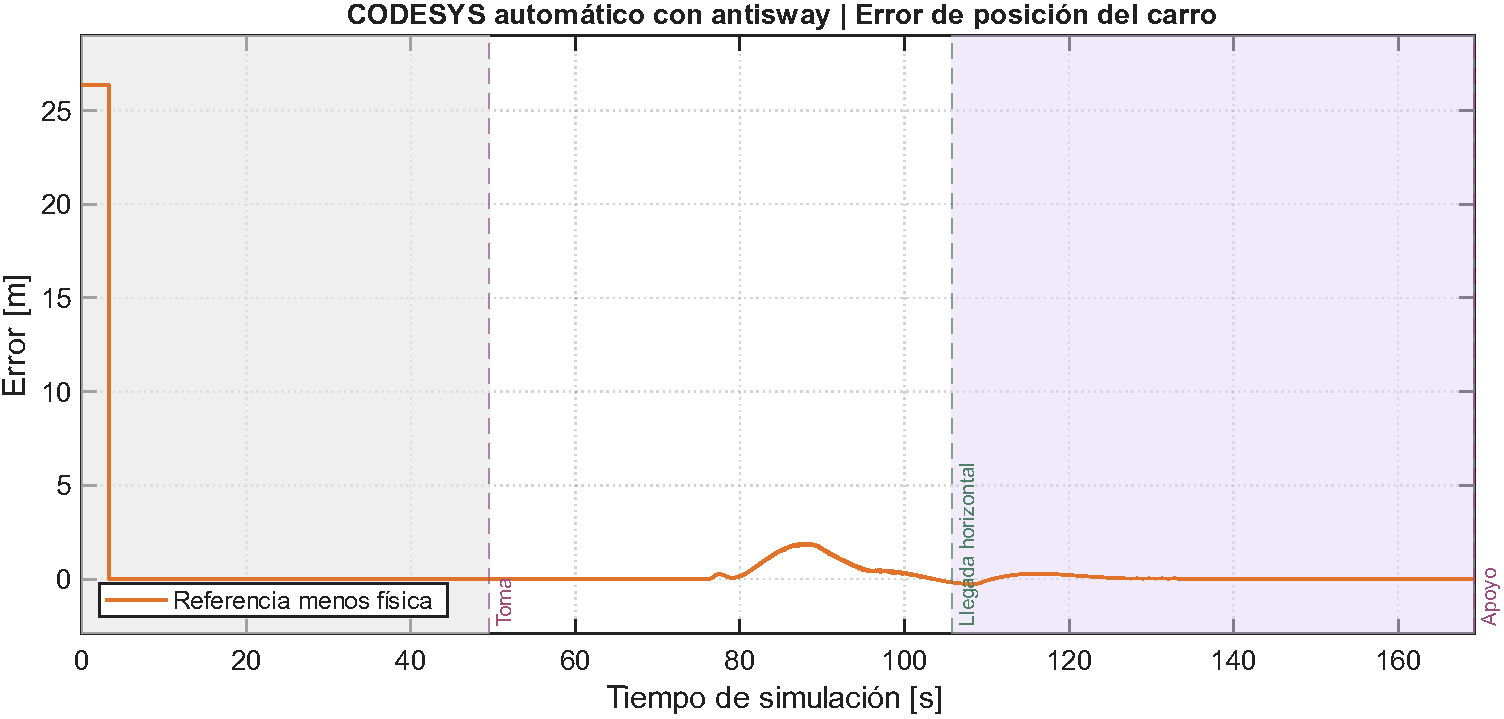
\includegraphics[width=0.98\textwidth]{graficas_individuales/automatico_con_ex.pdf}
\caption{CODESYS automático con antisway: Error horizontal, calculado como referencia menos posición física.}\label{fig:individual_automatico_con_ex}
\end{figure}

\begin{figure}[!htbp]
\centering
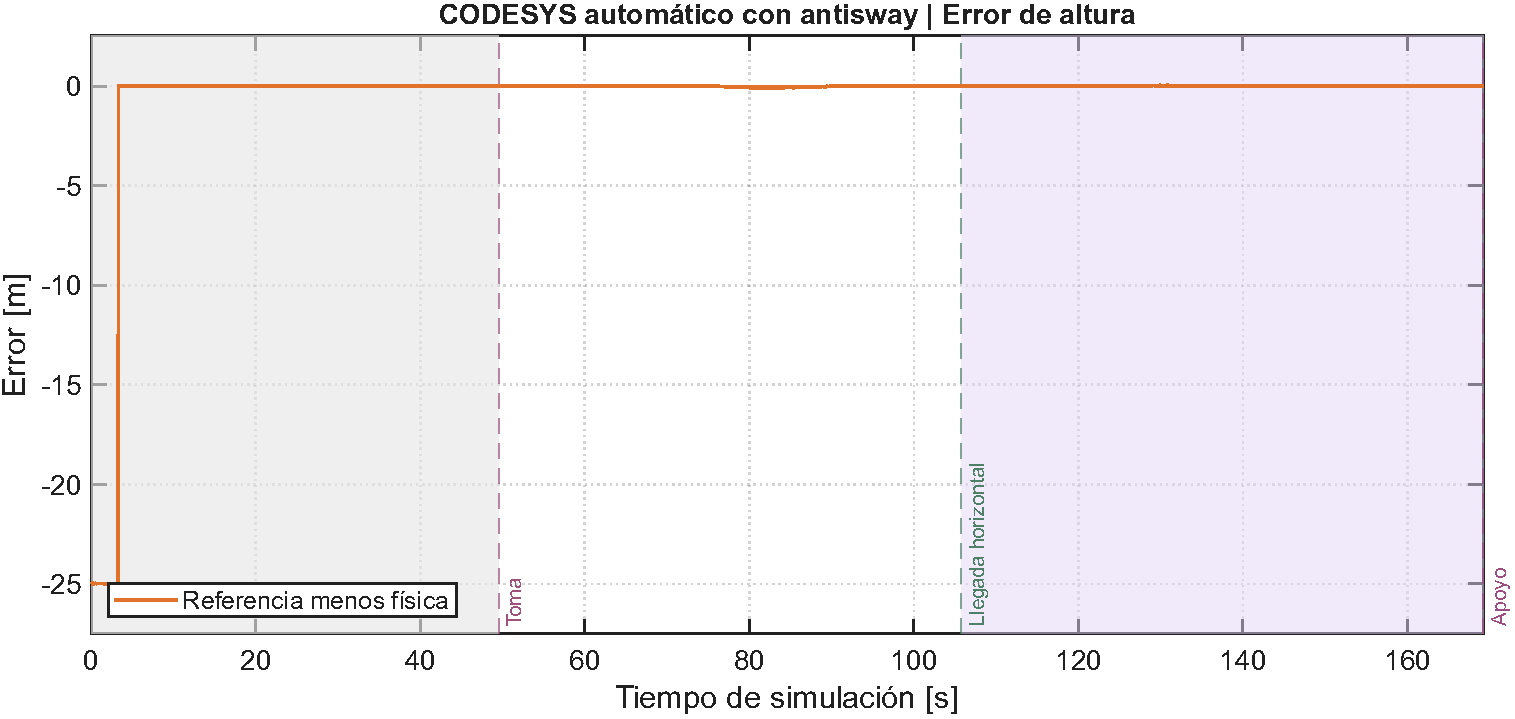
\includegraphics[width=0.98\textwidth]{graficas_individuales/automatico_con_ey.pdf}
\caption{CODESYS automático con antisway: Error de altura, calculado como referencia menos altura física.}\label{fig:individual_automatico_con_ey}
\end{figure}

\begin{figure}[!htbp]
\centering
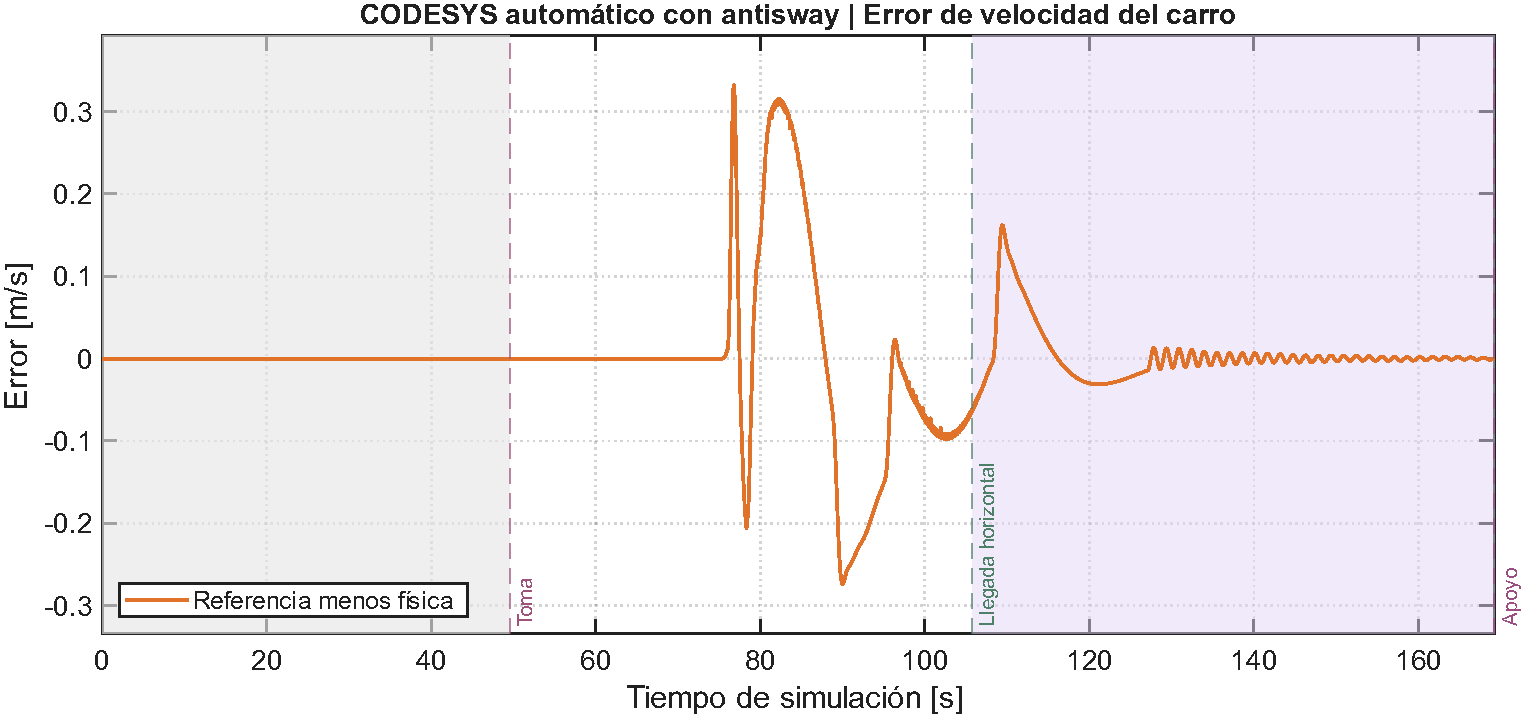
\includegraphics[width=0.98\textwidth]{graficas_individuales/automatico_con_evx.pdf}
\caption{CODESYS automático con antisway: Error de velocidad del carro, calculado como referencia menos velocidad física.}\label{fig:individual_automatico_con_evx}
\end{figure}

\begin{figure}[!htbp]
\centering
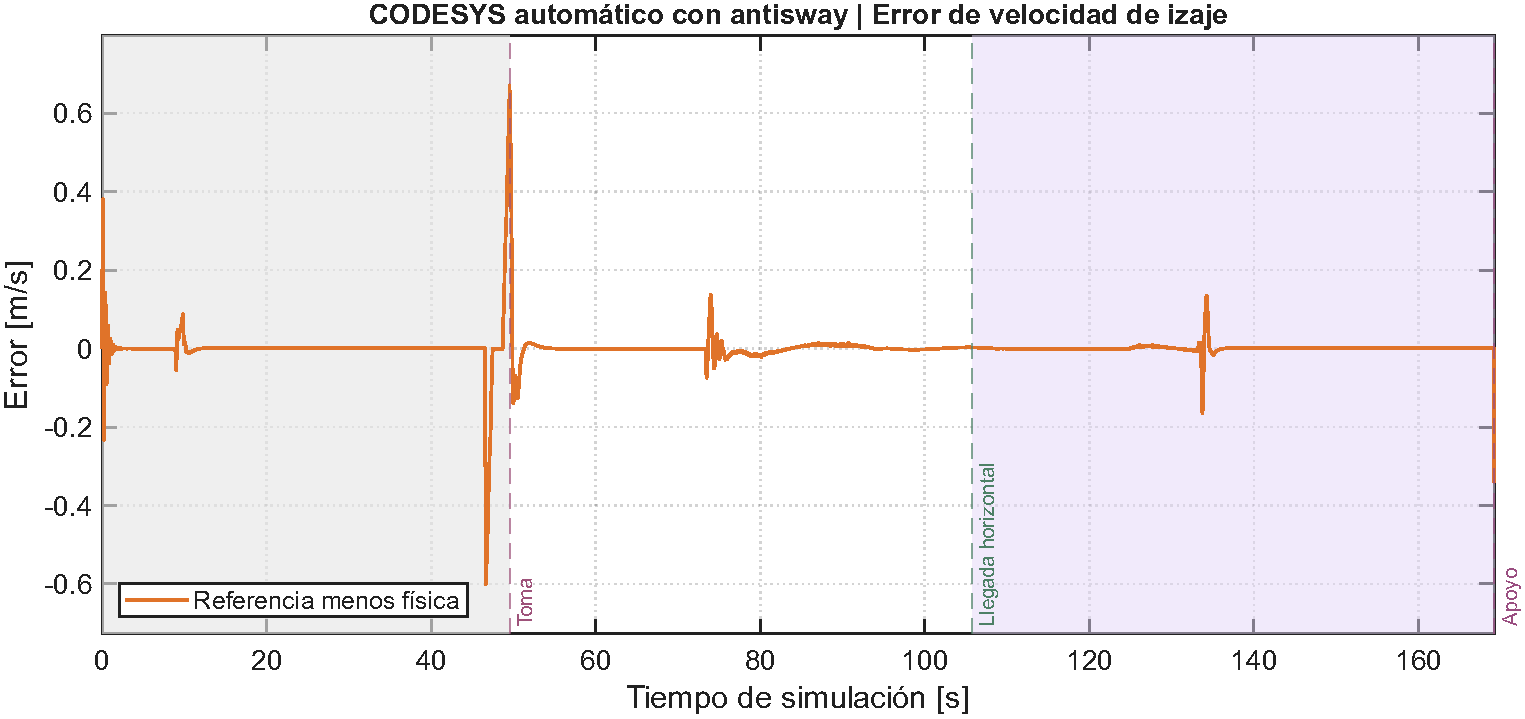
\includegraphics[width=0.98\textwidth]{graficas_individuales/automatico_con_evy.pdf}
\caption{CODESYS automático con antisway: Error de velocidad de izaje, calculado como referencia menos velocidad física.}\label{fig:individual_automatico_con_evy}
\end{figure}

\begin{figure}[!htbp]
\centering
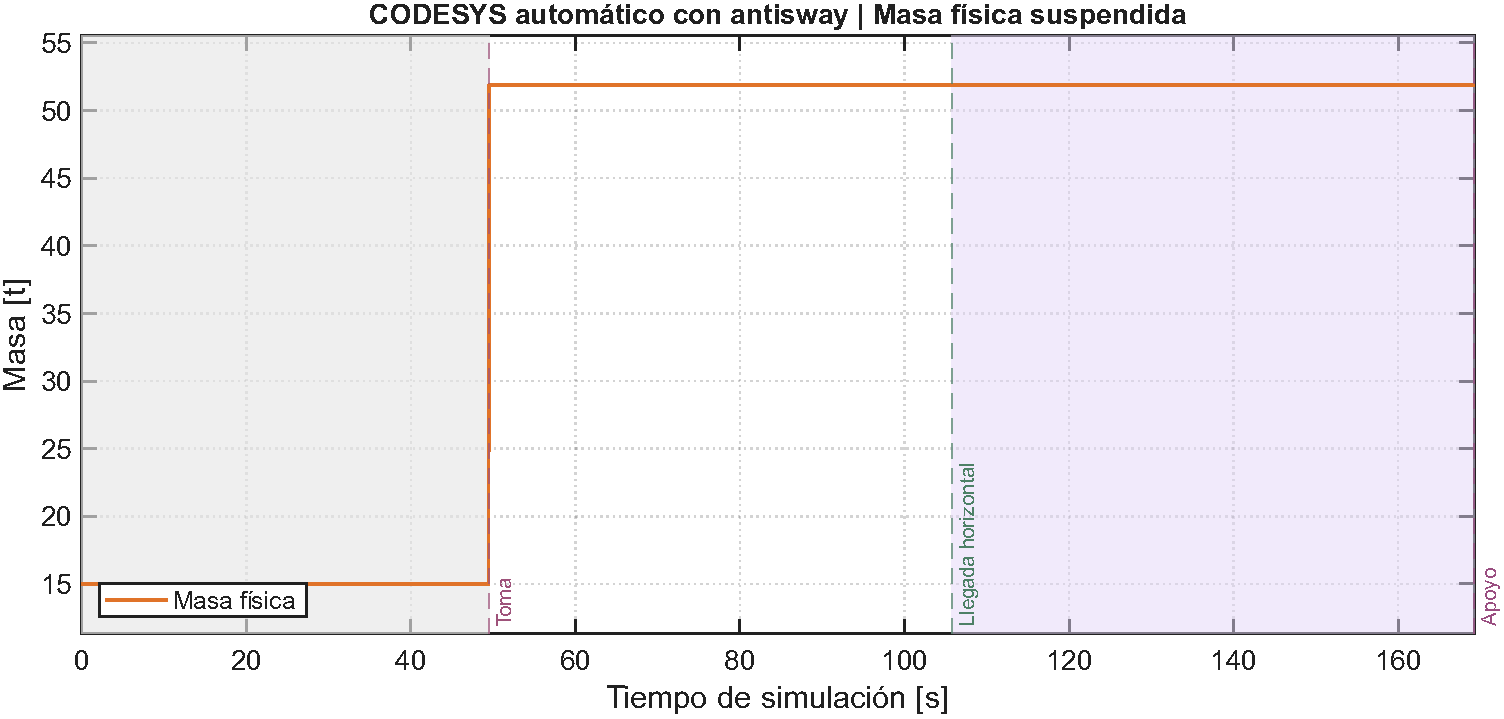
\includegraphics[width=0.98\textwidth]{graficas_individuales/automatico_con_masa.pdf}
\caption{CODESYS automático con antisway: Masa física suspendida: 51,863 t representa conjunto cargado y 15 t corresponde al spreader vacío.}\label{fig:individual_automatico_con_masa}
\end{figure}

\begin{figure}[!htbp]
\centering
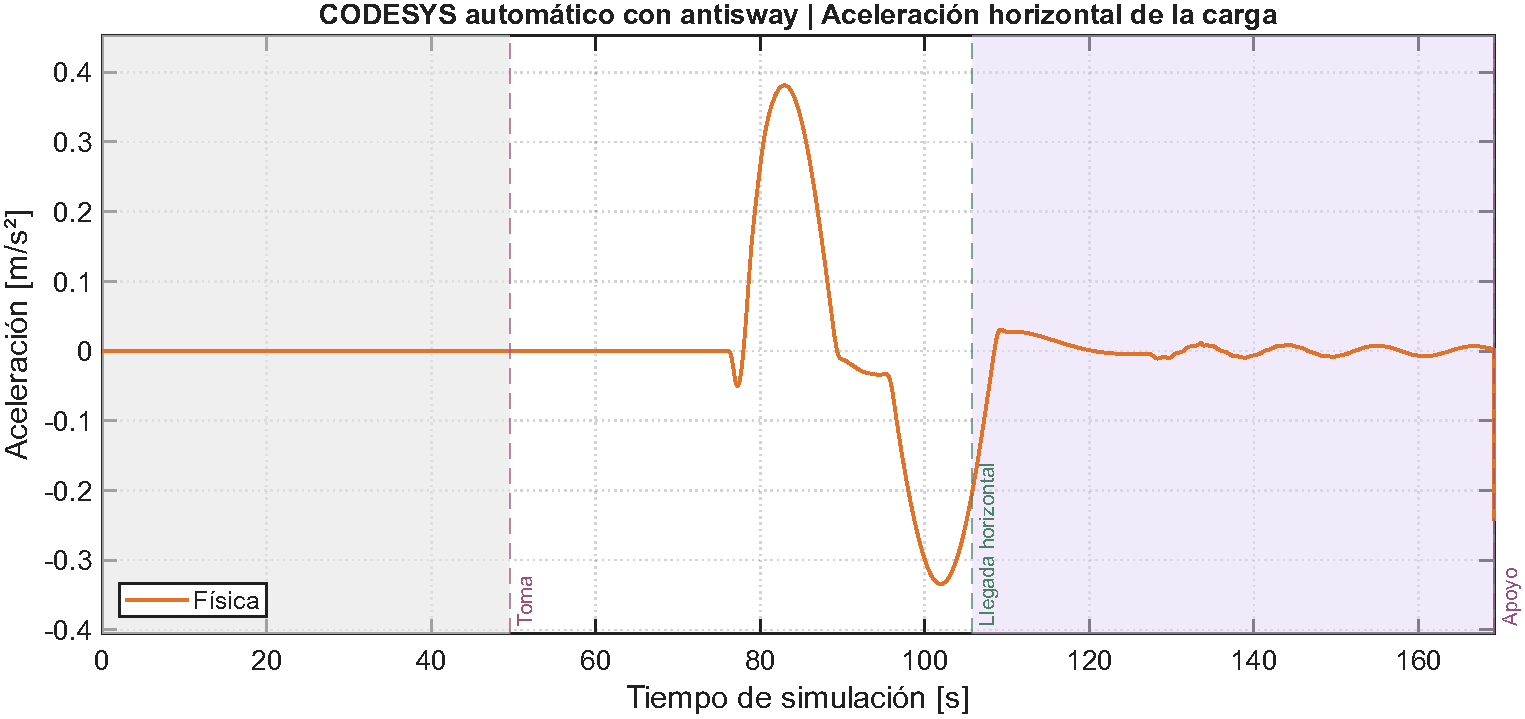
\includegraphics[width=0.98\textwidth]{graficas_individuales/automatico_con_ax_carga.pdf}
\caption{CODESYS automático con antisway: Aceleración horizontal física de la carga; se conservan las oscilaciones registradas.}\label{fig:individual_automatico_con_ax_carga}
\end{figure}

\clearpage
\section{Comparación experimental entre CODESYS manual y automático}
\label{sec:comparacion_ensayos_codesys}
\subsection{Resultados físicos de las cuatro pruebas}
La \cref{tab:resultado_cuatro_codesys} resume las corridas actuales. Sólo CODESYS manual con antisway completó la entrega. Las dos pruebas sin antisway terminaron con carga retenida en la zona de cruce; CODESYS automático con antisway alcanzó apoyo pero conservó la carga física. Las duraciones de parada por límite o diagnóstico no son tiempos de ciclo productivo y no permiten ordenar las implementaciones por rendimiento.

\begin{table}[!htbp]\centering\small
\caption{Estado final y resultado de las cuatro pruebas actualizadas.}\label{tab:resultado_cuatro_codesys}
\begin{tabular}{L{.28\textwidth}C{.10\textwidth}C{.15\textwidth}L{.35\textwidth}}\toprule
Prueba & Fin [s] & Masa final [kg] & Resultado\\\midrule
CODESYS manual sin antisway & 187.20 & 51\,863 & Sin entrega; parada solicitada. Registro nativo parcial.\\
CODESYS manual con antisway & 169.20 & 15\,000 & Entrega física confirmada y parada.\\
CODESYS automático sin antisway & 180.00 & 51\,863 & Sin entrega; límite programado.\\
CODESYS automático con antisway & 279.52 & 51\,863 & Apoyo alcanzado; descarga física bloqueada; parada diagnóstica.\\\bottomrule
\end{tabular}\end{table}

Las trayectorias absolutas de la \cref{fig:individual_comparacion_x,fig:individual_comparacion_y,fig:individual_comparacion_theta,fig:individual_comparacion_masa} conservan cada duración. Su superposición ilustra el resultado y los distintos finales; no calcula RMS de un ciclo completo frente a otro incompleto. Las comparaciones cuantitativas de etapas deben limitarse a fases completadas por ambas variantes, como la toma y el despegue. La espera prolongada y el apoyo bloqueado se interpretan como diagnóstico, sin incorporarlos como mejora aparente del RMS ni como entregas completadas.

\begin{figure}[!htbp]
\centering
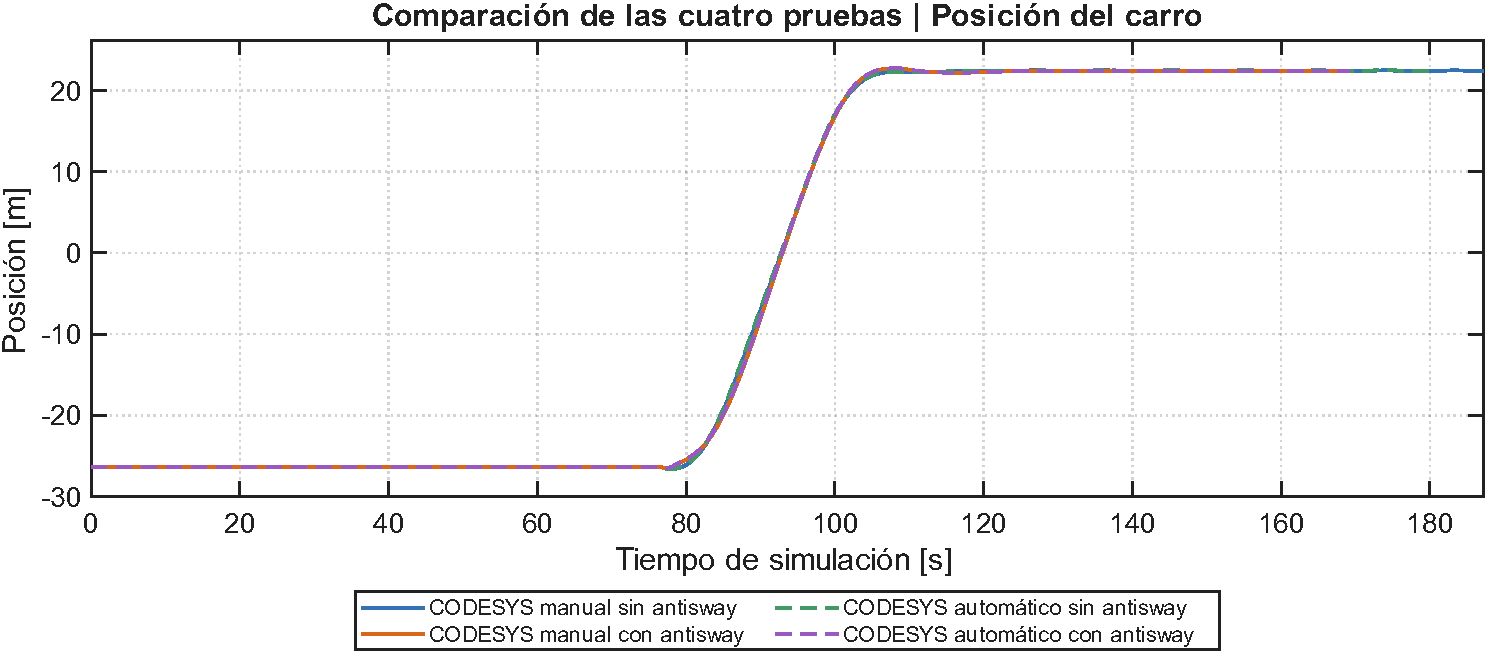
\includegraphics[width=0.98\textwidth]{graficas_individuales/comparacion_x.pdf}
\caption{Comparación de las cuatro pruebas: posición del carro. Las curvas con antisway terminan en el apoyo o intento de entrega: 168,92 s para CODESYS manual y 169,24 s para CODESYS automático. Las variantes sin antisway conservan su duración y cobertura disponibles.}\label{fig:individual_comparacion_x}
\end{figure}

\begin{figure}[!htbp]
\centering
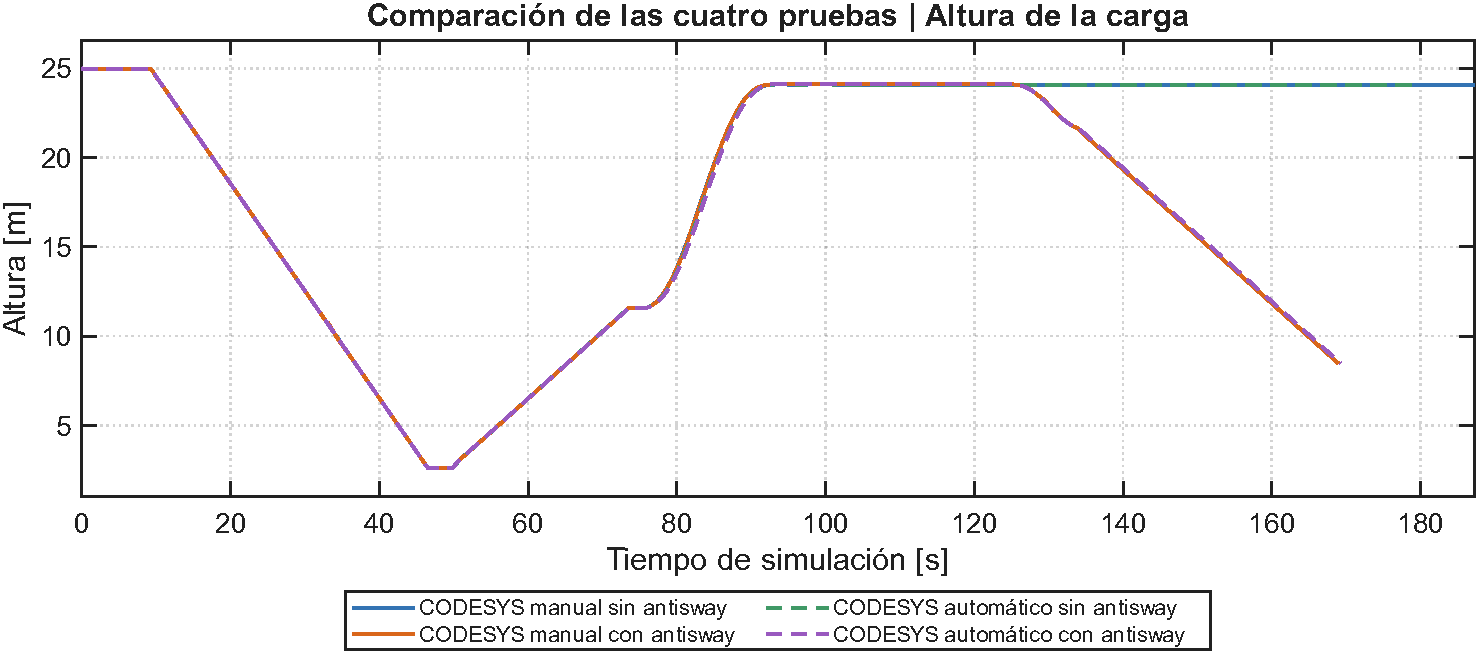
\includegraphics[width=0.98\textwidth]{graficas_individuales/comparacion_y.pdf}
\caption{Comparación de las cuatro pruebas: altura de la carga. Las curvas con antisway terminan en el apoyo o intento de entrega: 168,92 s para CODESYS manual y 169,24 s para CODESYS automático. Las variantes sin antisway conservan su duración y cobertura disponibles.}\label{fig:individual_comparacion_y}
\end{figure}

\begin{figure}[!htbp]
\centering
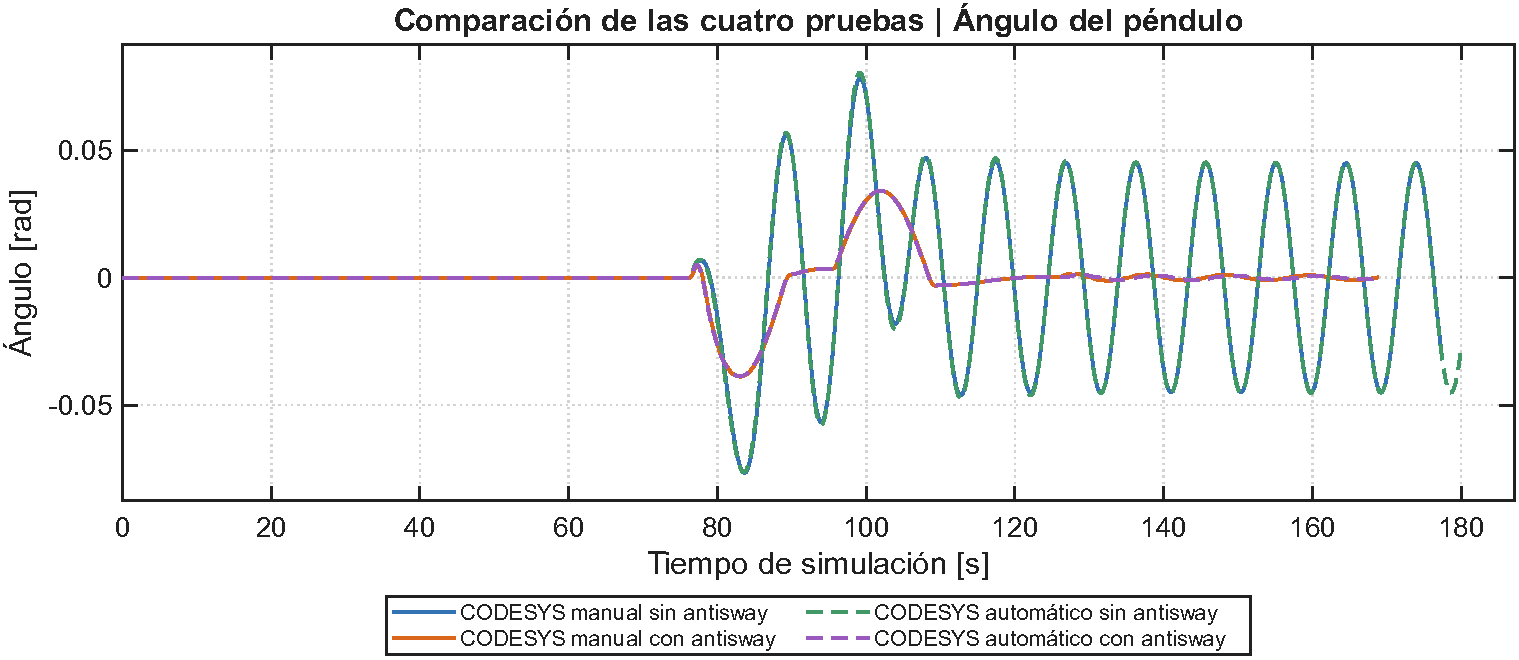
\includegraphics[width=0.98\textwidth]{graficas_individuales/comparacion_theta.pdf}
\caption{Comparación de las cuatro pruebas: ángulo del péndulo. Las curvas con antisway terminan en el apoyo o intento de entrega: 168,92 s para CODESYS manual y 169,24 s para CODESYS automático. Las variantes sin antisway conservan su duración y cobertura disponibles.}\label{fig:individual_comparacion_theta}
\end{figure}

\begin{figure}[!htbp]
\centering
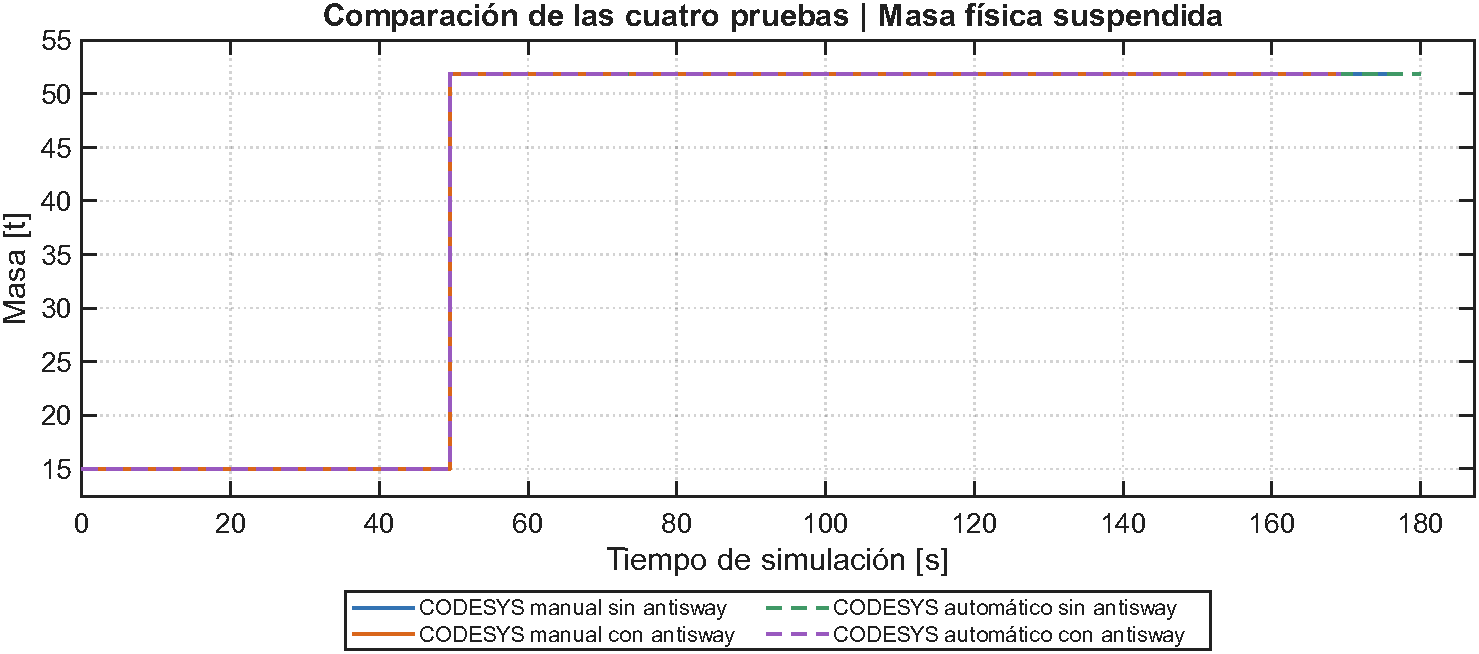
\includegraphics[width=0.98\textwidth]{graficas_individuales/comparacion_masa.pdf}
\caption{Comparación de las cuatro pruebas: masa física suspendida. Las curvas con antisway terminan en el apoyo o intento de entrega: 168,92 s para CODESYS manual y 169,24 s para CODESYS automático. Las variantes sin antisway conservan su duración y cobertura disponibles.}\label{fig:individual_comparacion_masa}
\end{figure}

\begin{figure}[!htbp]
\centering
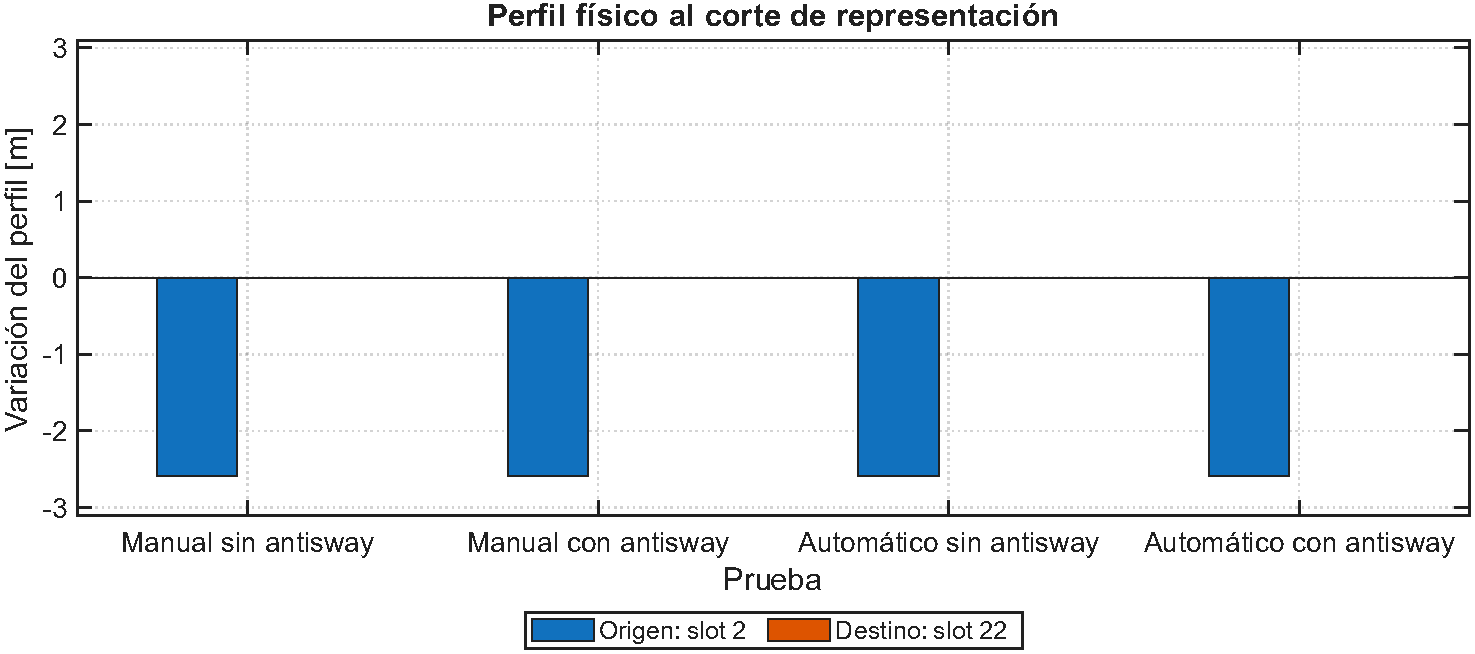
\includegraphics[width=0.98\textwidth]{graficas_individuales/perfil.pdf}
\caption{Variación del perfil físico hasta el final del intervalo graficado. Se observa el retiro en origen; el corte de las variantes con antisway se realiza antes de la confirmación de descarga. La entrega posterior de CODESYS manual con antisway se conserva como resultado del registro completo en el texto.}\label{fig:actual_perfil}
\end{figure}

\subsection{Seguridad observada y límites de interpretación}
Desde START hasta fin no se registraron fallas de PLC ni emergencias en las cuatro maniobras; las paradas incompletas no fueron abortos por fallo del PLC. La vigilancia de comunicación se mantiene independiente del reloj de la planta. Esta observación nominal no sustituye pruebas de emergencia, límites últimos, congelamiento del enlace o sobrevelocidad.

El margen geométrico mínimo aproximado en automático fue $2.658~\mathrm{m}$ para CODESYS manual con antisway, $2.626~\mathrm{m}$ para CODESYS automático sin antisway y $2.668~\mathrm{m}$ para CODESYS automático con antisway. Se calcula con huella rectangular y perfil físico, sin inclinación; el canal dedicado de colisión no estuvo disponible. Por ello no se certifica ausencia dinámica de colisiones. Se ocultó únicamente el mensaje de colisión de la HMI; no se anuló la lógica ni se convirtió un valor no disponible en cero.

\subsection{Cobertura y método de representación}
Los modos de funcionamiento se describen en el texto y no se grafican ni se marcan sobre los ejes. Cada figura contiene una sola gráfica. Por criterio de representación, todas las curvas temporales de CODESYS manual con antisway terminan en el apoyo a $168.92~\mathrm{s}$ y las de CODESYS automático con antisway en el intento de entrega a $169.24~\mathrm{s}$. Las dos variantes sin antisway conservan su duración completa, respetando su cobertura registrada. Los resultados finales de entrega y bloqueo se obtienen del registro completo posterior al corte, que permanece intacto; la masa graficada hasta el apoyo todavía incluye el contenedor. Las bandas grises muestran el intervalo previo a la toma confirmada y las bandas lavanda el tramo posterior a la llegada horizontal; las marcas corresponden a eventos físicos. La aceleración de izaje se presenta en escala completa y, por separado, con zoom vertical de $-1$ a $+1~\mathrm{m/s^2}$, sin alterar ni filtrar los datos. Las gráficas conservan los tiempos originales de las señales físicas, del controlador y de los torques. Las referencias, monitores y errores procesados se representan por tiempo sobre una rejilla de $40~\mathrm{ms}$, con interpolación para señales continuas y retención previa para estados discretos. Los tramos fuera de cobertura se excluyen. Se distinguen referencias, consignas y señales físicas, conservando los transitorios de contacto, elasticidad y arranque. La velocidad angular de referencia es una derivada numérica sobre la rejilla de análisis; la velocidad angular física es nativa.

CODESYS manual sin antisway sufrió interrupción de registro por almacenamiento: control y monitores hasta $130.72~\mathrm{s}$, numerosas señales físicas hasta $177.305~\mathrm{s}$, telemetría de operador hasta $187.20~\mathrm{s}$. Esta telemetría permite documentar la posición y el estado final, pero no recuperar el torque ni demostrar máximos nativos del tramo ausente. Las otras tres pruebas conservan registro nativo hasta la parada; las señales constantes de inicialización se identifican como constantes, sin exigirles una muestra final artificial.

Cada prueba conserva video de visualización y HMI. En CODESYS manual sin antisway, la captura cada $0.52~\mathrm{s}$ produce 180 s de reproducción para $187.20~\mathrm{s}$ simulados: prevalece el reloj de simulación. El retardo de redibujo impide utilizar la captura final como evidencia única de parada o descarga.



\clearpage
\section{Discusión}
El modelo conserva las principales características no lineales de la planta y permite estudiar la interacción entre el movimiento del carro, la elasticidad del cable y el balanceo. La separación jerárquica simplifica la interpretación: los reguladores resuelven seguimiento, el supervisor resuelve la secuencia y el nivel de seguridad decide si el movimiento está permitido.

La planificación basada en el perfil relevado evita depender de una geometría fija del barco. El operador entrega la posición horizontal final y el sistema calcula la cota de aproximación. Sin embargo, la validez de esta estrategia depende de completar el barrido y de mantener actualizado el perfil ante cada toma o descarga.

La decisión de reducir la acción anti-sway durante el crucero es un compromiso entre producción y oscilación. No se elimina la protección geométrica ni se supera la velocidad de diseño. La corrección se reactiva antes de descender, por lo que el posicionamiento final conserva un requisito angular estricto.

\subsection{Limitaciones del modelo}
El contacto se representa mediante rigidez concentrada y el viento no se modela explícitamente. Los accionamientos se aproximan mediante moduladores de torque de primer orden. El LIDAR se obtiene de una tabla ideal y no incluye ruido, pérdidas de lectura ni oclusiones. Estas simplificaciones son adecuadas para verificar la arquitectura, aunque una validación posterior debería incorporar incertidumbres y retardos de comunicación.

% IMAGEN A INSERTAR: diagrama de limitaciones y futuras mejoras del modelo.
\figplaceholder{Esquema de los fenómenos modelados y los fenómenos simplificados.}{Alcance y limitaciones de la simulación.}


\section{Conclusiones}
Se obtuvo un modelo completo de una grúa portuaria STS en MATLAB, Simulink y Stateflow. La planta incluye la dinámica no lineal de la carga suspendida, elasticidad de cables, contacto, accionamientos, reductores, tambores, saturaciones y frenos. La correspondencia entre ecuaciones y subsistemas permite identificar el origen físico de cada señal.

El control regulatorio en cascada realiza el seguimiento del carro y compensa parte de su dinámica. El control de izaje mantiene la tensión y sigue perfiles verticales suaves. En la revisión vigente, la habilitación anti-sway mantiene la selección del operador durante el automático y el generador puede esperar estabilidad antes del descenso final.

El generador de trayectorias inicia izaje y traslación simultáneamente y aumenta la duración horizontal cuando el despeje todavía no es suficiente. La entrada y la altura de destino se calculan a partir de la envolvente local, la carga y el estiramiento del cable. Se conserva la línea global de dos alturas de contenedor como referencia visual y una cota alta de cruce dentro del generador.

El autómata supervisor organiza la operación, el barrido LIDAR, la toma, el pesaje, el automático, el descenso manual y la secuencia de frenos. El autómata de seguridad permanece separado y actúa ante límites últimos, exceso de velocidad, emergencia o pérdida de \textit{watchdog}. La estructura obtenida permite ejecutar y analizar una maniobra completa sin mezclar la lógica de producción con las protecciones.

% IMAGEN A INSERTAR: captura final de la carga depositada y el spreader retornando vacío.
\figplaceholder[0.50\textheight]{Captura final de la prueba: contenedor depositado en el barco y \textit{spreader} vacío en retorno.}{Resultado de la maniobra completa simulada.}


\clearpage
\section{Diccionario resumido de señales}
{\small
\renewcommand{\arraystretch}{1.10}
\begin{table}[H]
\centering
\caption{Señales principales del modelo.}
\begin{tabular}{L{4.3cm} L{2.4cm} L{7.0cm}}
\toprule
Señal & Unidad/tipo & Descripción\\
\midrule
$x_t$ & m & Posición horizontal del carro.\\
$v_t$ & m/s & Velocidad horizontal del carro.\\
$x_l,y_l$ & m & Posición del centro del cuerpo suspendido.\\
$l,l_h$ & m & Longitud geométrica y longitud comandada del cable.\\
$\theta_l$ & rad & Ángulo de balanceo respecto de la vertical.\\
$F_{hw}$ & N & Tensión equivalente por ramal.\\
$y_{c0}$ & m & Cota del perfil en la posición consultada.\\
\texttt{xRef}, \texttt{vxRef}, \texttt{axRef} & SI & Referencias del carro.\\
\texttt{yRef}, \texttt{vyRef}, \texttt{ayRef} & SI & Referencias del izaje.\\
\texttt{profileValid} & lógico & Confirma cobertura completa del barrido.\\
\texttt{loadedState} & lógico & Indica carga tomada desde DESPEGUE\_SUAVE; no implica pesaje completo.\\
\texttt{massEstimateValid} & lógico & Confirma que finalizó el pesaje.\\
\texttt{autoEntryHeightOK} & lógico & Perfil válido y altura medida suficiente según envolvente local.\\
\texttt{safetyEnvelope}\newline\texttt{Profile} & vector de 33 & Máximos locales del perfil y sus celdas vecinas.\\
\texttt{clearanceLineY} & m & Línea de seguridad calculada.\\
\texttt{swayControlEnable} & lógico & Habilitación efectiva de anti-sway.\\
\texttt{safetyPermitGlobal} & lógico & Permiso general del nivel 0.\\
\texttt{safetyPermitTrolley} & lógico & Permiso de movimiento horizontal.\\
\texttt{safetyPermitHoist} & lógico & Permiso de movimiento vertical.\\
\texttt{trackingFault} & lógico & Error de seguimiento sostenido.\\
\texttt{loadSequenceFault} & lógico & Falla de \textit{twistlocks} o secuencia de carga.\\
\texttt{watchdogToggle} & lógico & Pulso alternante del supervisor.\\
\bottomrule
\end{tabular}
\end{table}
}


\section{Índice compacto de funciones del supervisor}
\begin{table}[H]
\centering
\small
\caption{Funciones auxiliares implementadas dentro del supervisor.}
\begin{tabular}{L{5.2cm} L{8.5cm}}
\toprule
Función & Responsabilidad\\
\midrule
\texttt{procesarEntradasCrudas} & Detecta flancos, calcula aceleraciones, límites, torque comprobado y falla de seguimiento.\\
\texttt{registrarMuestraLidar} & Asigna una lectura al \textit{slot} y conserva la mayor cota.\\
\texttt{verificarCoberturaPerfil} & Comprueba que los 33 \textit{slots} tengan muestras.\\
\texttt{calcularVelocidadBarrido} & Genera velocidad limitada por distancia de frenado.\\
\texttt{calcularEnvolventeLocal} & Dilata el perfil mediante máximos de celdas vecinas.\\
\texttt{actualizarPerfilPorCarga} & Resta o suma una altura al tomar o liberar carga.\\
\texttt{calcularObjetivoSeguro} & Calcula altura local con carga, margen y estiramiento.\\
\texttt{retenerSolicitudHMI} & Memoriza la solicitud de barrido hasta atenderla o cancelarla.\\
\texttt{calcularFlagsSupervisor} & Calcula apoyo, intervención, reposo y proximidad al objetivo.\\
\texttt{calcularSuperficie}\newline\texttt{Objetivo} & Obtiene la mayor cota solapada por el contenedor.\\
\texttt{craneTrajectoryGenerator} & Planifica y evalúa los perfiles coordinados.\\
\texttt{cerrarLazoPosicionIzaje} & Corrige el error vertical final.\\
\texttt{referenciasManual} & Genera referencias manuales con rampas y saturaciones.\\
\texttt{referenciasBumpless} & Asegura continuidad durante los cambios de modo.\\
\texttt{referenciaDescensoFinal} & Mantiene el carro y permite descenso controlado.\\
\texttt{evaluarEstabilidad}\newline\texttt{Spreader} & Verifica ángulo y velocidad angular durante un tiempo.\\
\texttt{aplicarRetencionToma} & Inhibe movimientos hasta estabilizar después del cierre.\\
\texttt{detectarCuerdaFloja} & Aplica histéresis a la tensión del cable.\\
\texttt{calcularMandoManual} & Convierte \textit{joysticks} y aplica límites e interbloqueos.\\
\texttt{calcularDespeje} & Verifica línea de seguridad compensando estiramiento.\\
\texttt{calcularCodigos} & Codifica alarmas y fallas para el HMI.\\
\texttt{Estimar\_Masa} & Estima masa de contenedor a partir de la tensión.\\
\bottomrule
\end{tabular}
\end{table}


\section{Matriz de verificación propuesta}
{\small
\renewcommand{\arraystretch}{1.10}
\begin{table}[H]
\centering
\caption{Casos mínimos de verificación.}
\begin{tabular}{C{1.2cm} L{5.0cm} L{4.0cm} L{4.0cm}}
\toprule
ID & Caso & Estímulo & Resultado esperado\\
\midrule
V1 & Arranque normal & Marcha con permisos & Estado LISTO\\
V2 & Barrido completo & Orden de escaneo vacío & Perfil válido\\
V3 & Barrido con carga & Orden de escaneo cargado & No inicia\\
V4 & Toma estable & Contacto y cierre & Estado CARGADO\\
V5 & Toma inestable & Ángulo fuera de rango & Retiene cierre\\
V6 & Sobrepeso & $\widehat M_c>50000~\mathrm{kg}$ & Alarma y sin traslado\\
V7 & Automático sin perfil & Inicio automático & No ingresa\\
V8 & Trayectoria válida & Objetivo en barco & Sin colisión\\
V9 & Intervención manual & Mover \textit{joystick} & Salida bumpless\\
V10 & Descenso final & Ciclo automático completo & Solo mando vertical\\
V11 & Límite horizontal & Activar límite último & Emergencia carro\\
V12 & Límite vertical & Activar límite último & Emergencia izaje\\
V13 & Pulsador & Emergencia activa & Emergencia total\\
V14 & Watchdog congelado & Detener alternancia & Emergencia total\\
V15 & Reinicio inválido & Causa todavía activa & Permanece detenido\\
V16 & Retorno vacío & Objetivo en muelle & Admite automático sin carga\\
V17 & Altura local insuficiente & Inicio con perfil válido y altura baja & No ingresa a automático\\
V18 & Perfil después de toma/entrega & Cambio de \texttt{loadedState} & Resta/suma $2.59$ m en la celda\\
V19 & Espera previa al descenso & Velocidad o sway fuera de umbral & Retiene reloj del plan\\
\bottomrule
\end{tabular}
\end{table}
}


\section{Referencias}
\thispagestyle{mystyle}
{\small
\noindent [1] Universidad Nacional de Cuyo, Ingeniería Mecatrónica, ``317 -- Autómatas y Control Discreto. Proyecto Global Integrador 2025: Guía de trabajo Rev. 0 preliminar'', 2025.\par
\noindent [2] The MathWorks, Inc., \textit{Simulink User's Guide}, versión R2025b, 2025.\par
\noindent [3] The MathWorks, Inc., \textit{Stateflow User's Guide}, versión R2025b, 2025.\par
\noindent [4] K. Ogata, \textit{Ingeniería de control moderna}, 5.a ed. Pearson Educación, 2010.\par
\noindent [5] G. F. Franklin, J. D. Powell y A. Emami-Naeini, \textit{Feedback Control of Dynamic Systems}, 7.a ed. Pearson, 2015.\par
\noindent [6] W. Singhose, ``Command Shaping for Flexible Systems: A Review of the First 50 Years'', \textit{International Journal of Precision Engineering and Manufacturing}, vol. 10, n.º 4, pp. 153--168, 2009.\par
}

\end{document}
